% XeLaTeX can use any Mac OS X font. See the setromanfont command below.
% Input to XeLaTeX is full Unicode, so Unicode characters can be typed directly into the source.

% The next lines tell TeXShop to typeset with xelatex, and to open and save the source with Unicode encoding.

%!TEX TS-program = xelatex
%!TEX encoding = UTF-8 Unicode

\documentclass[11pt,twoside]{book}
\usepackage{multirow}
\usepackage{pdfpages}

\usepackage{geometry}                % See geometry.pdf to learn the layout options. There are lots.
%\usepackage[margin=1cm]{geometry}


%	\addtolength{\textwidth}{1.75in}
%
%	\addtolength{\topmargin}{-.875in}
%	\addtolength{\textheight}{1.75in}

\geometry{a4paper,left=20mm,top=20mm,total={162mm,230mm}}                   % ... or a4paper or a5paper or ... 
%\geometry{landscape}                % Activate for for rotated page geometry
%\usepackage[parfill]{parskip}    % Activate to begin paragraphs with an empty line rather than an indent

\setcounter{secnumdepth}{5}

\usepackage{amssymb}
%\usepackage{todonotes}
\setlength{\marginparwidth}{2cm}
\usepackage[backgroundcolor=white,bordercolor=blue,linecolor=blue,textwidth=1cm]{todonotes}
\usepackage{booktabs}
\usepackage{longtable}
\usepackage{url}

\usepackage[depth=4]{bookmark}


\usepackage{algorithm}
\usepackage{algpseudocode}

\usepackage{imakeidx}
\usepackage[utf8]{inputenc}
\usepackage[T1]{fontenc}
\makeindex[intoc]

\usepackage[font=normalsize]{caption}  

\usepackage{hyperref}
\hypersetup{
    colorlinks,
    citecolor=black,
    filecolor=black,
    linkcolor=black,
    urlcolor=black
}

\usepackage{xcolor}
\usepackage{listings}

\makeatletter
\global\let\tikz@ensure@dollar@catcode=\relax
\makeatother

\definecolor{mGreen}{rgb}{0,0.6,0}
\definecolor{mGray}{rgb}{0.5,0.5,0.5}
\definecolor{mPurple}{rgb}{0.58,0,0.82}
\definecolor{backgroundColour}{rgb}{0.95,0.95,0.92}
\definecolor{gray}{rgb}{0.4,0.4,0.4}
\definecolor{darkblue}{rgb}{0.0,0.0,0.6}
\definecolor{cyan}{rgb}{0.0,0.6,0.6}

\lstdefinestyle{CStyle}{
    backgroundcolor=\color{backgroundColour},   
    commentstyle=\color{mGreen},
    keywordstyle=\color{magenta},
    numberstyle=\tiny\color{mGray},
    stringstyle=\color{mPurple},
    basicstyle=\scriptsize\ttfamily,
    breakatwhitespace=false,         
    breaklines=true,                 
    captionpos=b,                    
    keepspaces=true,                 
    numbers=left,                    
    numbersep=5pt,                  
    showspaces=false,                
    showstringspaces=false,
    showtabs=false,                  
    tabsize=2,
    language=C
}


\lstset{ 
  backgroundcolor=\color{white},   % choose the background color; you must add \usepackage{color} or \usepackage{xcolor}; should come as last argument
  basicstyle=\footnotesize\ttfamily,        % the size of the fonts that are used for the code
  breakatwhitespace=false,         % sets if automatic breaks should only happen at whitespace
  breaklines=true,                 % sets automatic line breaking
  captionpos=b,                    % sets the caption-position to bottom
  commentstyle=\color{gray},    % comment style
  deletekeywords={...},            % if you want to delete keywords from the given language
  %escapeinside={\%*}{*)},          % if you want to add LaTeX within your code
  %extendedchars=true,              % lets you use non-ASCII characters; for 8-bits encodings only, does not work with UTF-8
  %firstnumber=1000,                % start line enumeration with line 1000
  frame=single,	                   % adds a frame around the code
  keepspaces=true,                 % keeps spaces in text, useful for keeping indentation of code (possibly needs columns=flexible)
  keywordstyle=\color{blue},       % keyword style
  language=C,                 % the language of the code
  %morekeywords={*,...},            % if you want to add more keywords to the set
  numbers=left,                    % where to put the line-numbers; possible values are (none, left, right)
  numbersep=5pt,                   % how far the line-numbers are from the code
  numberstyle=\tiny\color{gray}, % the style that is used for the line-numbers
  rulecolor=\color{black},         % if not set, the frame-color may be changed on line-breaks within not-black text (e.g. comments (green here))
  showspaces=false,                % show spaces everywhere adding particular underscores; it overrides 'showstringspaces'
  showstringspaces=false,          % underline spaces within strings only
  showtabs=false,                  % show tabs within strings adding particular underscores
  stepnumber=1,                    % the step between two line-numbers. If it's 1, each line will be numbered
  stringstyle=\color{black},     % string literal style
  tabsize=2,	                   % sets default tabsize to 2 spaces
}

\lstset{
  columns=fullflexible,
  showstringspaces=false,
  commentstyle=\color{gray}\upshape,
  backgroundcolor=\color{backgroundColour},   
  commentstyle=\color{mGreen},
  keywordstyle=\color{magenta},
  numberstyle=\tiny\color{mGray},
  stringstyle=\color{mPurple},
  basicstyle=\scriptsize\ttfamily,
  tabsize=2
}

\lstdefinelanguage{XML}
{
  morestring=[b]",
  morestring=[s]{>}{<},
  morecomment=[s]{<?}{?>},
  stringstyle=\color{black},
  identifierstyle=\color{darkblue},
  keywordstyle=\color{cyan},
  morekeywords={xmlns,version,type}% list your attributes here
}


% Will Robertson's fontspec.sty can be used to simplify font choices.
% To experiment, open /Applications/Font Book to examine the fonts provided on Mac OS X,
% and change "Hoefler Text" to any of these choices.

\renewcommand{\scriptsize}{\tiny}

\usepackage{fontspec,xltxtra,xunicode}
\defaultfontfeatures{Mapping=tex-text}
\setromanfont[Scale=MatchLowercase,Mapping=tex-text]{Optima}
\setsansfont[Scale=MatchLowercase,Mapping=tex-text]{Optima}
\setmonofont[Scale=MatchLowercase]{Andale Mono}

%%%% Graphics
\usepackage{graphicx}
\usepackage{tikz}
\definecolor{unilublue}{RGB}{55,149,218}
\definecolor{sntred}{RGB}{219,46,27}
\definecolor{sntpurple}{RGB}{86,30,130}
%\definecolor{sntblue}{RGB}{50,130,207}
\definecolor{sntblue}{RGB}{55,149,218}

\pgfdeclareimage[width=30mm]{logo-snt}{logos/logo-snt}
\pgfdeclareimage[width=30mm]{logo-uni-lu}{logos/logo-uni-lu}

%%%% Fancy
\usepackage{fancyhdr}

%%%% Increase page length
\addtolength{\textheight}{1in}

%%%% Sections
\usepackage{xspace}
\usepackage{sectsty}
\allsectionsfont{\sffamily}

\setlength{\parskip}{1em}

%\renewcommand{\,}{$^{\cdot}$}

%%%% Title
\newcommand{\titleone}{\textsf{FR}}
\newcommand{\titletwo}{\textsf{Final Report}}
\newcommand{\titlethree}{\textsf{}}

\newcommand{\todoinline}[1]{\todo[color=orange,inline]{ \textbf{TODO}: #1 }}

\newcommand{\TODO}[1]{\todo[color=orange,inline]{ \textbf{TODO}: #1 }}
\newcommand{\DONE}[1]{\todo[color=green,inline]{ \textbf{DONE}: #1 }}


\usepackage{amsmath}
\usepackage{array}
\usepackage{lipsum}

\usepackage{algorithm}
\usepackage{algpseudocode}

\newcommand{\LXS}{LXS}
\newcommand{\GSL}{GSL}
\newcommand{\ESA}{ESA}
\newcommand{\FIXME}[1]{\textcolor{red}{#1}}

\newcommand{\CHANGED}[1]{{#1}}
\newcommand{\CHANGEDTWO}[1]{{#1}}
\newcommand{\CHANGEDOCT}[1]{{#1}}
\newcommand{\CHANGEDNOV}[1]{{#1}}

\newcommand{\TRFOUR}[1]{{#1}}

\newcommand{\STARTCHANGEDNOV}{\color{black}}
\newcommand{\ENDCHANGEDNOV}{\color{black}}


\newcommand{\STARTCHANGEDWPT}{\color{blue}}
\newcommand{\ENDCHANGEDWPT}{\color{black}}

\newcommand{\UPDATED}[1]{#1}

\newcommand{\D}[0]{$\Delta$}


%\newcommand{\MREVISION}[2]{\todo{\tiny{#1}}\textcolor{blue}{#2}}
\newcommand{\MREVISION}[2]{#2}

%\newcommand{\REVTWO}[2]{\todo[color=red]{\tiny{#1}}\textcolor{red}{#2}}
\newcommand{\REVTWO}[2]{#2}

\newcommand{\REVNOV}[2]{\textcolor{black}{#2}}

\newcommand{\REVTOOL}[2]{\todo[color=red]{\tiny{#1}}\textcolor{red}{#2}}

\newcommand{\JMR}[2]{\textcolor{black}{#2}}
\newcommand{\NEWFSCI}[1]{\textcolor{black}{#1}}

\newcommand{\JMRCHANGE}[1]{\textcolor{black}{#1}}
\newcommand{\UPDATE}[1]{\textcolor{black}{#1}}

\newcommand{\EMPH}[1]{\textbf{\emph{#1}}}
\newcommand{\INDEX}[1]{\index{\MakeLowercase{#1}}\EMPH{#1}}

\newcommand{\APPR}{\emph{MASS}\xspace}

\newcommand{\SAIL}{ESAIL\xspace}
\newcommand{\ESAIL}{ESAIL\xspace}

%\newcommand{\CITSAIL}{\cite{ESAIL}}

\begin{document}

\pagestyle{fancy}
\renewcommand{\sectionmark}[1]{\markright{\textit{#1}}}

\renewcommand{\headrulewidth}{2pt}% 2pt header rule
\renewcommand{\headrule}{\hbox to\headwidth{%
  \color{sntblue}\leaders\hrule height \headrulewidth\hfill}}

\fancyhf{}

%\lhead{\fancyplain{}{\setlength{\unitlength}{1mm}
%\begin{picture}(0,0)
%\put(0,-4){
\includegraphics[width=50pt]{logos/logo-snt}}
%\end{picture}}} 

\lhead{\fancyplain{}{\textit{}}}

\rhead{\fancyplain{}{\rightmark }}

\fancyfoot[C]{%
\begin{tikzpicture}[remember picture,overlay]
\path [fill=sntred]    ([xshift=88pt,yshift=20pt]current page.south west) rectangle
                       ([xshift=229pt,yshift=30pt] current page.south west);
\path [fill=sntpurple] ([xshift=229pt,yshift=20pt] current page.south west) rectangle
                       ([xshift=370pt,yshift=30pt] current page.south west);
\path [fill=sntblue]   ([xshift=370pt,yshift=20pt] current page.south west) rectangle
                       ([xshift=510pt,yshift=30pt] current page.south west);
\end{tikzpicture}
}

\fancyfoot[RO]{
\begin{tikzpicture}[remember picture,overlay]
\node [circle, ultra thick, fill=white, draw=sntblue] at ([xshift=530pt,yshift=35pt] current page.south west) {\thepage};
\end{tikzpicture}}

\fancyfoot[LE]{
\begin{tikzpicture}[remember picture,overlay]
\node [circle, ultra thick, fill=white, draw=sntblue] at ([xshift=65pt,yshift=35pt] current page.south west) {\thepage};
\end{tikzpicture}}



\newcommand{\prog}{P}
\newcommand{\prop}{}




\thispagestyle{empty}

\begin{tikzpicture}[remember picture,overlay]
\path [fill=sntred]    ([xshift=30pt,yshift=20pt]current page.south west) rectangle
                       ([xshift=210pt,yshift=50pt] current page.south west);
\path [fill=sntpurple] ([xshift=210pt,yshift=20pt] current page.south west) rectangle
                       ([xshift=390pt,yshift=50pt] current page.south west);
\path [fill=sntblue]   ([xshift=390pt,yshift=20pt] current page.south west) rectangle
                       ([xshift=570pt,yshift=51pt] current page.south west);
\path [fill=unilublue] ([xshift=30pt,yshift= 50pt] current page.south west) --
                       ([xshift=570pt,yshift= 50pt] current page.south west)
                       [rounded corners=20pt] --
                       ([xshift=570pt,yshift=740pt] current page.south west)
                       [sharp corners] --
                       ([xshift=30pt,yshift=740pt] current page.south west);
\node [fill=white,rounded corners=0pt,inner xsep=6pt,inner ysep=3pt]
      at ([xshift=523pt,yshift=120pt] current page.south west)
      {\pgfuseimage{logo-uni-lu}};

\node [fill=white,rounded corners=2pt,inner xsep=6pt,inner ysep=3pt]
      at ([xshift=520pt,yshift=780pt] current page.south west)
      {\pgfuseimage{logo-snt}};

%\node [circle, fill=white, draw=sntblue] at ([xshift=550pt,yshift=35pt] current page.south west) {a};

\node[draw=none,fill=none,right] at (-1, -7){\color{white}\LARGE\bf\titleone};
\node[draw=none,fill=none,right] at (-1, -8){\color{white}\LARGE\bf\titletwo};
\node[draw=none,fill=none,right] at (-1, -9){\color{white}\LARGE\bf\titlethree};

\node[draw=none,fill=none,right] at (-1, -12){\color{white}\Large\textsf{O. Cornejo, F. Pastore, E. Viganò}};
\node[draw=none,fill=none,right] at (-1, -13){\color{white}\Large\textsf{Interdisciplinary Centre for Security, Reliability and Trust}};
\node[draw=none,fill=none,right] at (-1, -14){\color{white}\Large\textsf{University of Luxembourg}};
\node[draw=none,fill=none,right] at (11, -16){\color{white}\textsf{ITT-1-9873-ESA-FAQAS-SUTP}};
\node[draw=none,fill=none,right] at (11, -17){\color{white}\Large\textsf{Issue 4, Rev. 1}};
\node[draw=none,fill=none,right] at (11, -18){\color{white}\Large\textsf{\today}};
\node[draw=none,fill=none,right] at (-1, -24){\color{white}\tiny\textsf{EUROPEAN SPACE AGENCY. CONTRACT REPORT.}};
\node[draw=none,fill=none,right] at (-1, -24.3){\color{white}\tiny\textsf{The work described in this report was done under ESA contract. Responsibility for the contents resides in the author or organisation that prepared it.}};
\node[draw=none,fill=none,right] at (-1, -24.8){\color{white}\tiny\textsf{The copyright in this document is vested in the University of Luxembourg.}};
\node[draw=none,fill=none,right] at (-1, -25.1){\color{white}\tiny\textsf{This document may only be reproduced in whole or in part, or stored in a retrieval system,or transmitted in any form, or by any means electronic,}};
\node[draw=none,fill=none,right] at (-1, -25.4){\color{white}\tiny\textsf{mechanical, photocopying or otherwise, either with the prior permission of the University of Luxembourg or in accordance with the terms of ESTEC Contract No. 4000128969/19/NL/AS.}};

\node[draw=none,fill=none,right] at (-1, -24){\color{white}\tiny\textsf{EUROPEAN SPACE AGENCY. CONTRACT REPORT.}}; 
\node[draw=none,fill=none,right] at (-1, -24.3){\color{white}\tiny\textsf{The work described in this report was done under ESA contract. Responsibility for the contents resides in the author or organisation that prepared it.}};
\node[draw=none,fill=none,right] at (-1, -24.8){\color{white}\tiny\textsf{The copyright in this document is vested in the University of Luxembourg.}};
\node[draw=none,fill=none,right] at (-1, -25.1){\color{white}\tiny\textsf{This document may only be reproduced in whole or in part, or stored in a retrieval system,or transmitted in any form, or by any means electronic,}}; 
\node[draw=none,fill=none,right] at (-1, -25.4){\color{white}\tiny\textsf{mechanical, photocopying or otherwise, either with the prior permission of the University of Luxembourg or in accordance with the terms of ESTEC Contract No. 4000128969/19/NL/AS.}};


\end{tikzpicture}

\newpage


% !TEX root = MAIN.tex

\section*{Revisions}
\label{sec:revisions}


\setlength\LTleft{0pt}
\setlength\LTright{0pt}
\tiny 
%@{\extracolsep{\fill}}
\begin{longtable}{|p{2cm}|p{1cm}|p{1.5cm}|p{9cm}|@{}}
\label{table:codeoperators} \\
\hline
\textbf{Issue Number}&\textbf{Date}&\textbf{Authors}&\textbf{Description}\\
\hline
ITT-1-9873-ESA-FAQAS-FR
Issue 1 Rev. 1&
October 29th, 2021&
Fabrizio Pastore, Oscar Cornejo, Enrico Viganò&
\begin{minipage}{8cm}
Initial release.
\end{minipage}
\\
\hline
ITT-1-9873-ESA-FAQAS-FR
Issue 1 Rev. 2&
November 11th, 2021&
Fabrizio Pastore, Oscar Cornejo, Enrico Viganò&
\begin{minipage}{8cm}
Added Chapter~\ref{chap:deliverables_summary} (deliverables summary).\\
Added Chapter~\ref{ch:toolset} (description of toolset package).\\
Added information about input and outputs of the tools in Chapter~\ref{chapter:methodology} (see blue text).
\end{minipage}
\\
\hline
                                                    
\end{longtable}
\normalsize

\clearpage

% !TEX root = MAIN.tex

\section*{Delivered Items}
\label{sec:deliverables}

In the following Table we provide a list of deliverable items released with this document. Each Item is identified by it's path on the Alfresco system.

\setlength\LTleft{0pt}
\setlength\LTright{0pt}
\tiny 
%@{\extracolsep{\fill}}
\begin{longtable}{|p{9cm}|p{6cm}@{}}
\label{table:deliverables} \\
\hline
\textbf{Deliverable}&Description\\
\hline
ASN1CC-CaseStudy/Specifications/ACN-UM-v-3-2.pdf&User manual of ASN1 Compiler\\
ASN1CC-CaseStudy/Specifications/taste-documentation-current.pdf&Taste software documentation including ASN1 overview\\
\hline
GSL-CaseStudies/Specifications/gs-man-nanosoft-ms100-command-and-management-sdk-3.6.2-1-g67fe6e1.pdf&LXS softwrae specifications\\
\hline
LXS-CaseStudies/Specifications&Folder with LXS specifications\\
LXS-CaseStudies/Specifications/FAQAS-LXS-MAN-001\_1- SVF Software Installation and User Manual.pdf&SVF and ESAIL Software Installation and User Manual\\
LXS-CaseStudies/Specifications/ESAIL-LXS-ICD-P-0184\_2A ADCS IF SW External ICD.docx&\\
LXS-CaseStudies/Specifications/ESAIL-LXS-SDD-P-0105\_1B On-board Application Software Design Document&\\
LXS-CaseStudies/Specifications/MOC-applicable MIB egos-mcs-s2k-icd-0001-version7.0-FINAL&SCOS-2000 Database Import ICD\\
LXS-CaseStudies/Specifications/ocp.dat&SCOS-2000 Database file containing the specifications of the nominal value ranges for ESAIL ADCS parameters.\\
\hline
SnT-Software/FAQAS-DataDrivenMutator-Buffers.zip&Preliminary implementation of the data-driven mutation testing component\\
%\begin{minipage}{8cm}
%Initial release.
%\end{minipage}
\\
\hline

%ITT-1-9873-ESA-FAQAS-D1
%Issue 4
%&DATE
%&Fabrizio Pastore, Oscar Cornejo
%&
%\begin{minipage}{8cm}
%\end{minipage}
%\\

%\hline
                                                    
\end{longtable}
\normalsize

\clearpage



\tableofcontents



% !TEX root = MAIN.tex

\section{Introduction}
\label{sec:introduction}
\addcontentsline{toc}{chapter}{Introduction}

%This document is the summary report of the ESA activity ITT-1-9873-ESA, which concerns the development of a framework for the automated assessment and the automated improvement of test suites for space software\footnote{In this report, we use the term space software to indicate software to be deployed on hardware that runs on-orbit.}.
 
From spacecrafts to ground stations, software has a prominent role in space systems; for this reason, the success of space missions depends on the quality of the system hardware as much on the dependability of its software. Mission failures due to insufficient software sanity checks~\cite{Schiaparelli} are unfortunate examples, pointing to the necessity for systematic and predictable quality assurance procedures in space software. 


Since one of the primary objectives of software testing is to identify the presence of software faults, an effective way to assess the quality of a test suite consists of artificially injecting faults in the software under test and verifying the extent to which the test suite can detect them. 
This approach is known as \emph{mutation analysis}~\cite{DeMillo78}. 
In mutation analysis, faults are automatically injected in the program through automated procedures referred to as mutation operators. Mutation operators enable the generation of faulty software versions that are referred to as \emph{mutants}.  
Mutation analysis helps evaluate the effectiveness of a test suite, \JMRCHANGE{for a specific software system,} based on its mutation score, which is the percentage of mutants leading to test failures. Also, mutation analysis enables \emph{mutation testing}, which concerns the automated generation of test cases that discover mutants.

Despite its potential, mutation analysis is not widely adopted by industry. The main reasons include its limited scalability and the pertinence of the mutation score as an adequacy criterion~\cite{papadakis2016threats}. Indeed, for a large software system, the number of generated mutants might prevent the execution of the test suite against all the mutated versions. Also, the generated mutants might be either 
semantically equivalent to the original software~\cite{madeyski2013overcoming} or redundant with each other~\cite{Shin:TSE:DCriterion:2018}. Equivalent and redundant mutants may bias the mutation score as an adequacy criterion. 
Finally, test generation approaches are preliminary and cannot be applied in industrial space context. For example, they can generate test inputs only for batch programs that can be compiled with the LLVM infrastructure~\cite{chekam2021killing}.

%The mutation analysis literature has proposed several optimizations to address problems related to scalability and mutation score pertinence~\cite{zhang2013operator,gopinath2015hard,zhang2013faster,grun2009impact,schuler2010covering,schuler2013covering,schuler2009efficient}. 
%However, these approaches 
%have not been evaluated on industrial, embedded systems
%and there are no feasibility studies concerning the integration of such optimizations and their resulting, combined benefits.
%Also, existing mutation analysis approaches cannot identify problems related to the interoperability of integrated components (integration testing), which is a major problem in 
%Cyber-physical Systems~\cite{Givehchi:2017,Jirkovsk:2017} and, consequently, space software --- mainly due to the wide variety and heterogeneity of the technologies and standards adopted.

The FAQAS activity addresses the problems above. It is a joint work between the SnT Centre of the University of Luxembourg\footnote{https://wwwen.uni.lu/snt}, Gomspace Luxembourg\footnote{https://gomspace.com/} (GSL) and OHB Luxspace\footnote{https://luxspace.lu/} (LXS).
FAQAS led to the development of a toolset that addresses the challenges above. It includes four tools:
\EMPH{MASS} (Mutation Analysis for Space Software), 
\EMPH{DAMAt} (DAta-driven Mutation Analysis with Tables), 
\EMPH{SEMuS} (Symbolic Execution-based MUtant analysis for Space software),
and \EMPH{DAMTE} (DAta-driven Mutation TEsting).



% of code-driven mutation analysis in the space context. The evaluation has shown that the most effective solutions to improve scalability and mutation score accuracy are mutants sampling and equivalence metrics based on compiler optimizations, respectively. To guarantee a scalable mutation testing process and the accurate computation of the mutation score, mutants sampling should be based on sequential analysis relying on fixed-width sequential confidence interval, a research discovery done within FAQAS.
%
%•	An empirical evaluation demonstrating the feasibility of data-driven mutation analysis with space software.
%•	The definition of an approach for code-driven mutation testing that relies on symbolic execution to identify test inputs that enable killing mutants not killed by the test suite under analysis.
%•	Demonstrating the feasibility of automated test generation for mutation testing based on symbolic execution. More precisely, symbolic execution can be successfully used to select test inputs that kill live mutants within unit test cases. However, unsurprisingly, it cannot be adopted when, to kill a mutant, it is necessary to rely on external components (e.g., networks or simulators), in such cases, which are common for integration and system test suites, symbolic execution alone is insufficient to generate test cases (e.g., because it cannot translate the simulator logic into an SMT formula to derive test cases from).
%\item The definition of guidelines for the adoption of mutation analysis and testing strategies within ECSS activities. The proposed guidelines support both quality assurance activities described in ECSS standards and Independent Software Verification and Validation (ISVV) practices.
%\end{itemize}

\begin{figure*}[tb]
\begin{center}
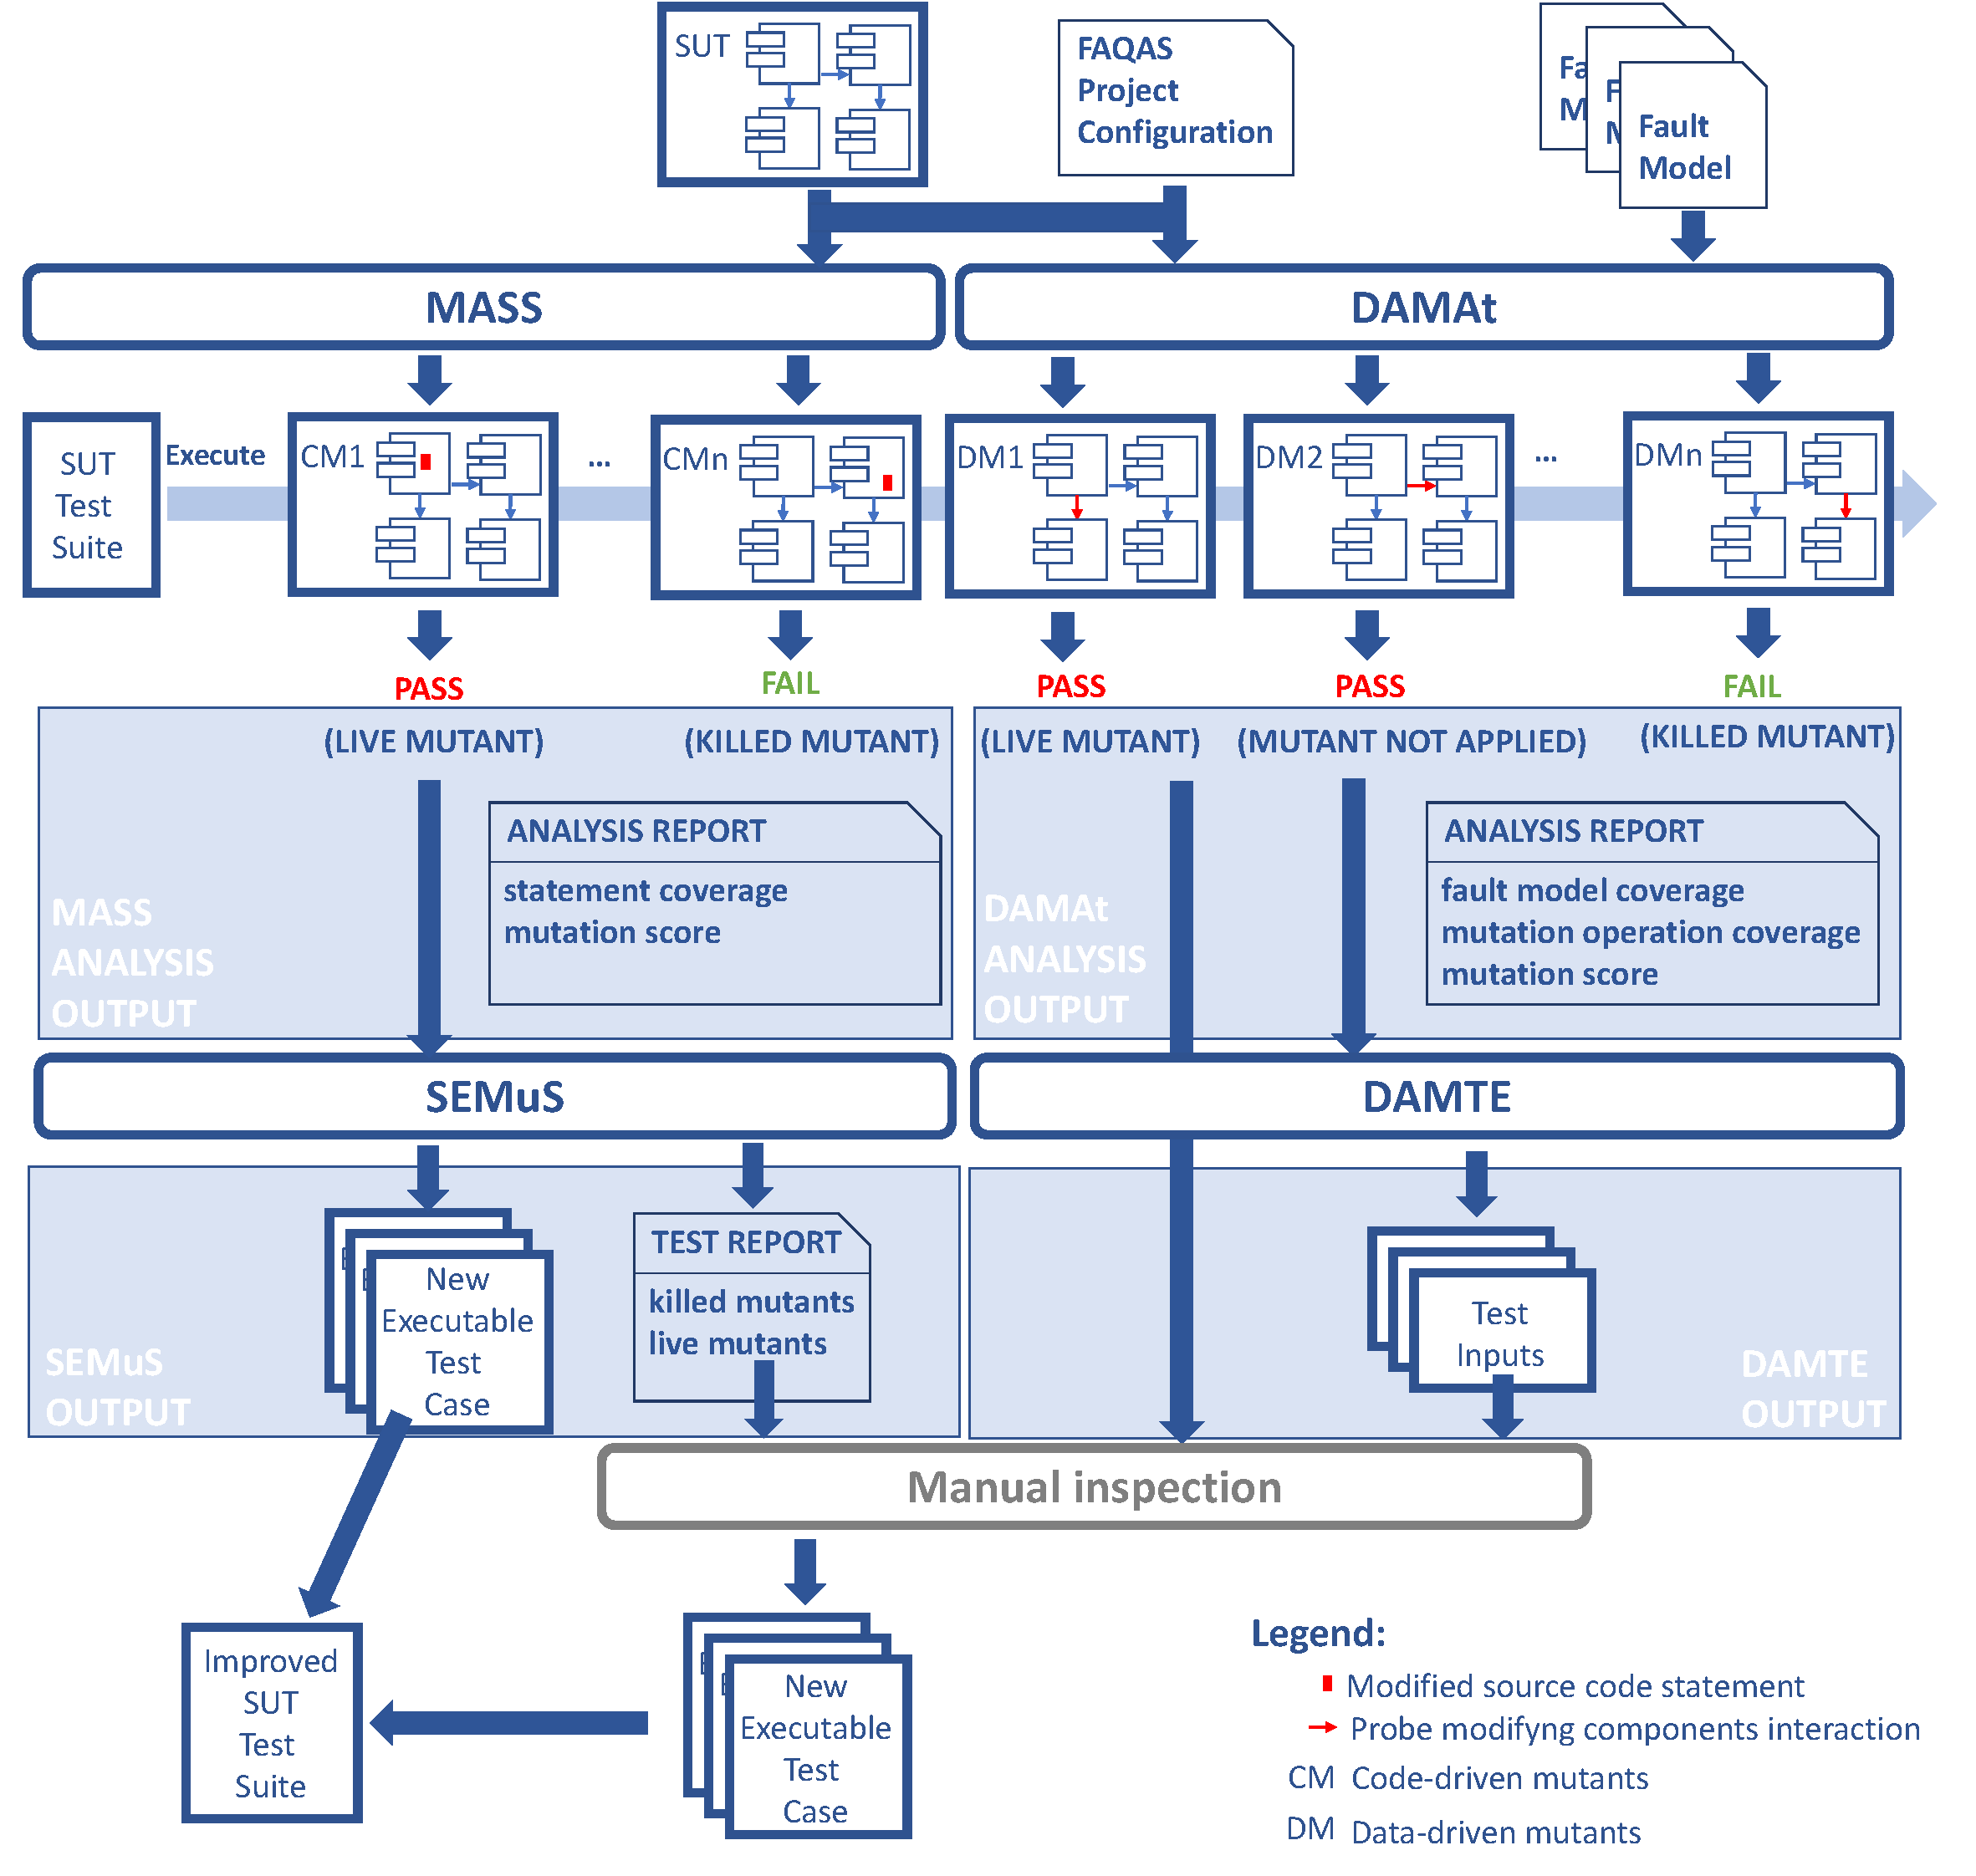
\includegraphics[width=0.7\textwidth]{images/FAQAS-overview.pdf}
\caption{Overview of the FAQAS toolset}
\label{fig:FAQAS:toolset}
\end{center}
\end{figure*}

Figure~\ref{fig:FAQAS:toolset} provides an overview of the input and outputs of the FAQAS toolset. It relies on the idea of generating multiple modified versions of the software system under test (SUT), some are derived by modifying the implementation of the software (code-driven mutants) other by integrating a mutation API that alters the messages exchanged by the software components of the SUT (data-driven mutants). 
The SUT test suite shall be executed with all the mutants, if it is effective then it shall fail with each of them. The mutants for which a failure is not observed are said to be \EMPH{live} and indicate a pitfall in the test suite.
All the FAQAS tools take as input the software under test (SUT), its test suite, and a set of configuration files. 

\EMPH{MASS} generates code-driven mutants. It integrates a pipeline of solutions that make mutation analysis feasible with large SUT. The three main contributions of MASS are (1) the automated identification of trivially equivalent mutants using an ensemble of compiler optimization options, (2) the computation of the mutation score based on mutant sampling with fixed size confidence interval approach (FSCI), (3) the automated identification of equivalent mutants based on coverage. 
MASS reports the set of live mutants, the set of killed mutants (i.e., mutants that are discovered by the test suite), and information useful to draft a verification report, which includes the statement coverage of the SUT test suite and the mutation score (i.e., the percentage of mutants discovered by the test suite).

\EMPH{DAMAt} generates mutants for data-driven mutation analysis. Data-driven mutation analysis is a research contribution of FAQAS. Instead of mutating the implementation of the SUT, it consists of altering the data exchanged by software components. 
DAMAt relies on fault models that specify how to mutate the data exchanged by software components through data-driven mutation operators. DAMAt can automatically alter data that is stored in data buffers (e.g., before serialization on the communication channel).
DAMAt enables the simulation of faults that affect simulated components (e.g., sensors), which is not feasible with traditional, code-driven mutation analysis. 
DAMAt generates as output a set of killed mutants (i.e., mutants that, during testing, successfully alter the data, and lead to test case failures), a set of live mutants (i.e., mutants that, during testing, successfully alter the data, but do not lead to test case failures), and a set of mutants not applied (i.e., mutants that, during testing, could not alter any data because the data they target is never exercised by the SUT); also, it provides information useful to draft a verification report, which includes the fault model coverage (i.e., percentage of fault models with at least one mutant applied), the mutation operation coverage (i.e., percentage of mutants applied), and the mutation score.

\EMPH{SEMuS} automatically generates executable unit test cases based on code-driven mutation analysis results. The generated unit test cases detect mutants not detected by the original test suite. The generated test cases include test oracles that shall be manually validated by engineers, which enables detecting faults. The generated test cases can be integrated into regression test suites.

SEMuS takes as input the list of live mutants detected by MASS. It generates a set of additional test cases that can be integrated into the SUT test suite. Also, it reports the list of killed mutants and the list of mutants that remain live (i.e., for which SEMuS did not generate a test case that kill them). Live mutants shall be manually inspected by engineers to either determine if they are equivalent or to manually derive a test case capable of killing them.

\EMPH{DAMTE} is a manual procedure supported by an automated symbolic execution toolset; it automatically identifies the test inputs that make software components exchange the data targeted by data-driven mutation operators. The derived test inputs can then be manually integrated into the SUT test suite.
 
The activity also included an extensive empirical evaluation demonstrating the feasibility, effectiveness, and scalability of the proposed toolsets in the space context, as described in the following sections.
 
%FAQAS.drawio.pdf

%Sections~\ref{ch:mass:approach} to~\ref{sec:data:test_suite_augmentation} provide an overview of the FAQAS tools: MASS, SEMuS, DAMAt, and DAMTE.
%Section~\ref{chapter:caseStudies} introduces the case study subjects considered for empirical evaluation.
%Section~\ref{sec:summary:results} provides an overview of the empirical results obtained.
%Section~\ref{sec:conclusion} concludes this report.



%% !TEX root = MAIN.tex

\section{Acronyms and Abbreviations}
\label{sec:acronyms}


%@{\extracolsep{\fill}}
\begin{tabular}{|p{1.5cm}|p{14.5cm}|}
%&\TODO{Add acronyms. OSCAR: I've add some...} \\

%ACO & Ant Colony Optimization\\
D1& Deliverable 1 of FAQAS activity, \emph{Analysis and Survey of Mutation Testing}\\
D2& Deliverable 2 of FAQAS activity, \emph{Study of Mutation Testing Applicability to Space Software}\\
FOM & First Order Mutant\\
HOM & Higher-Order Mutant\\
LOC & Lines of Code\\
%SBST & Search Based Software Testing\\
%Fabrizio: we cannot use SE as acronym
%SE & Symbolic Execution\\
SOM & Second Order Mutant\\
SUT & Software Under Test\\
TS & Test Suite\\
UL HPC & University of Luxembourg High Performance Computing

%Comment #2:
%When generating the pdf file, make sure to have the index of the document on the left, so that the document is easier to navigate.
%Author: Pedro Barrios Subject: Sticky Note Date: 28/02/2020, 09:18:06
%Comment #3:
%Try to make the document a bit more friendly to read (e.g. by adding some sentences in bold (see the highlighted ones for this paragraph), making bigger
%separation between paragraphs, ...)
%Author: Pedro Barrios Subject: Sticky Note Date: 28/02/2020, 09:18:11
%Comment #4:
%It is perhaps interesting to add a chapter with some basic definitions?
%e.g. equivalent mutant, redundant mutant, mutation score, killed mutant, live mutant, weak mutation, ...
%Author: Pedro Barrios Subject: Sticky Note Date: 28/02/2020, 09:18:18
%Comment #5:
%Please, consider to add more examples.

                                                           
\end{tabular}
\normalsize

\clearpage

% !TEX root =  Main.tex
\chapter{State-of-the-art}
\label{ch:stateOfTheArt}

%\item The literature on mutation analysis/testing mostly focuses on modifying the code of the software under test (hereafter, code-driven approaches). Some approaches rely on modifying models, but they aim to generate test cases not assessing test suites. There are no approaches that assess test suites by changing the data generated by software components (hereafter, data-driven approaches).
%\item The mutation operators widely adopted to perform code-driven mutation analysis are the sufficient set of operators and the set of deletion operators. Other operators did not receive the same degree of attention in the literature. For example, higher-order mutation operators are reported to be easier to kill than the first-order ones (i.e., they are less effective in assessing test suites limitations); consequently, they had been adopted less in empirical studies.                   
%o	The literature lacks mutation analysis approaches that enable simulating errors in the presence of simulated components (e.g., sensors). 
%o	Scalable approaches targeting mutation testing (i.e., automatically generating test cases that kill mutants) are few. The most promising ones rely on symbolic execution based on LLVM, which might be inapplicable for onboard flight software compiled for specific architectures. 

This chapter briefly discusses the applicability, in the context of space software, of existing solutions related to the four contributions of FAQAS: code-driven mutation analysis, 
code-driven mutation testing, data-driven mutation analysis, 
data-driven mutation testing.

\section{Code-driven mutation analysis}
\label{sec:background}

Mutation analysis can drive the generation of test cases, which is referred to as \INDEX{mutation testing} in the literature.
A detailed overview of mutation testing and analysis solutions and optimizations can be found in recent surveys~\cite{jia2010analysis,papadakis2019mutation}.

\subsection{Mutation Adequacy and Mutation Score computation}
\label{background:adequacy}
A mutant is said to be killed if at least one test case in the test suite fails when exercising the mutant.
Mutants that do not lead to the failure of any test case are said to be live.
Three conditions should hold for a test case to kill a mutant: \emph{reachability} (i.e, the test case should execute the mutated statement), \emph{necessity} (i.e., the test case should reach an incorrect intermediate state after executing the mutated statement), and \emph{sufficiency} (i.e., the final state of the mutated program should differ from that of the original program)~\cite{offutt1997automatically}.

The mutation score, i.e., the percentage of killed mutants, is a quantitative measure of the quality of a test suite. Recent studies have shown that achieving a high mutation score improves significantly the fault detection capability of a test suite
~\cite{papadakis2018mutation},  
\JMR{1.6}{
a result which contrasts with that of structural coverage measures~\cite{Chekam:17}. However, a very high mutation score (e.g., above 75\%) is required to achieve a higher fault detection rate than the one obtained with other coverage criteria, such as statement and branch coverage~\cite{Chekam:17}. In other words, there exists a strong association between a high mutation score and a high fault revelation capability for test suites.}
 

The capability of a test case to kill a mutant also depends on the observability of the program state. To overcome the limitations due to observability, different strategies to identify killed mutants can be adopted; they are known as strong, weak, firm, and flexible mutation coverage~\cite{ammann2016introduction}. 
\JMR{1.11 3.9}{With strong mutation, to kill a mutant, there shall be an observable difference between the outputs of the original and mutated programs.  
With weak mutation, the state (i.e., the valuations of the program variables in scope) of the mutant shall differ from the state of the original program, after the execution of the mutated statement~\cite{Lee1994}. 
With firm mutation, the state of the mutant shall differ from the state of the original program at execution points between the first execution of the mutated statement and the termination of the program~\cite{Woodward88}. 
Flexible mutation coverage consists of checking if the mutated code leads to object corruption~\cite{mateo2012validating}}.
For space software, we suggest to rely on strong mutation because it is the only criterion that truly assesses the fault detection capability of the test suite; indeed, it relies on a mutation score that reflects the percentage of mutants leading to test failures. With the other mutation coverage criteria, a mutant is killed if the state of the mutant after  execution of the mutated statement differs from the one observed with the original code, without any guarantee that either the erroneous values in state variables will propagate or the test oracles will detect them. 




\subsection{Mutation Operators}
\label{sec:related:operators}

%% !TEX root =  ../Main.tex

\newcommand{\op}{\mathit{op}}
\newcommand{\ArithmeticSet}{ \texttt{+}, \texttt{-}, \texttt{*}, \texttt{/}, \texttt{\%} }
\newcommand{\LogicalSet}{ \texttt{&&}, \texttt{||} }
\newcommand{\RelationalSet}{ \texttt{>}, \texttt{>=}, \texttt{<}, \texttt{<=}, \texttt{==}, \texttt{!=} }
\newcommand{\BitWiseSet}{ \texttt{\&}, \texttt{|}, \land }
\newcommand{\ShiftSet}{ \texttt{>>}, \texttt{<<} }


\begin{table}[h]
\caption{Implemented set of mutation operators.}
\label{table:operators} 
\centering
\scriptsize
\begin{tabular}{|@{}p{4mm}@{}|@{}p{2cm}@{\hspace{1pt}}|@{}p{11.1cm}@{}|}
\hline
&\textbf{Operator} & \textbf{Description$^{*}$} \\
\hline
\multirow{7}{*}{\rotatebox{90}{\emph{Sufficient Set}}}&ABS               & $\{(v, -v)\}$	\\
\cline{2-3}
&AOR               & $\{(\op_1, op_2) \,|\, \op_1, \op_2 \in \{ \ArithmeticSet \} \land \op_1 \neq \op_2 \} $       \\
&    			  & $\{(\op_1, \op_2) \,|\, \op_1, \op_2 \in \{\texttt{+=}, \texttt{-=}, \texttt{*=}, \texttt{/=}, \texttt{\%} \texttt{=}\} \land \op_1 \neq \op_2 \} $       \\
\cline{2-3}
&ICR               & $\{i, x) \,|\, x \in \{1, -1, 0, i + 1, i - 1, -i\}\}$           \\
\cline{2-3}
&LCR               & $\{(\op_1, \op_2) \,|\, \op_1, \op_2 \in \{ \texttt{\&\&}, || \} \land \op_1 \neq \op_2 \}$            \\
&				  & $\{(\op_1, \op_2) \,|\, \op_1, \op_2 \in \{ \texttt{\&=}, \texttt{|=}, \texttt{\&=}\} \land \op_1 \neq \op_2 \}$            \\
&				  & $\{(\op_1, \op_2) \,|\, \op_1, \op_2 \in \{ \texttt{\&}, \texttt{|}, \texttt{\&\&}\} \land \op_1 \neq \op_2 \}$            \\
\cline{2-3}
&ROR               & $\{(\op_1, \op_2) \,|\, \op_1, \op_2 \in \{ \RelationalSet \}\}$            \\
&				  & $\{ (e, !(e)) \,|\, e \in \{\texttt{if(e)}, \texttt{while(e)}\} \}$ \\
\cline{2-3}
&SDL               & $\{(s, \texttt{remove}(s))\}$            \\
\cline{2-3}
&UOI               & $\{ (v, \texttt{--}v), (v, v\texttt{--}), (v, \texttt{++}v), (v, v\texttt{++}) \}$            \\   
\hline
\hline
\multirow{5}{*}{\rotatebox{90}{\emph{OODL}}}&AOD               & $\{((t_1\,op\,t_2), t_1), ((t_1\,op\,t_2), t_2) \,|\, op \in \{ \ArithmeticSet \} $       \\ 
\cline{2-3}
&LOD               & $\{((t_1\,op\,t_2), t_1), ((t_1\,op\,t_2), t_2) \,|\, op \in \{  \} \}$       \\ 
\cline{2-3}
&ROD               & $\{((t_1\,op\,t_2), t_1), ((t_1\,op\,t_2), t_2) \,|\, op \in \{ \RelationalSet \} \}$       \\ 
\cline{2-3}
&BOD               & $\{((t_1\,op\,t_2), t_1), ((t_1\,op\,t_2), t_2) \,|\, op \in \{ \BitWiseSet \} \}$       \\ 
\cline{2-3}
&SOD               & $\{((t_1\,op\,t_2), t_1), ((t_1\,op\,t_2), t_2) \,|\, op \in \{ \ShiftSet \} \}$       \\ 
%\hline
%COR               & $\{(\op_1, \op_2) \,|\, \op_1, \op_2 \in \{ \texttt{\&\&}, \texttt{||}, \land \} \land \op_1 \neq \op_2 \}$            \\
\hline
\hline
\multirow{3}{*}{\rotatebox{90}{\emph{Other}}}&LVR			& $\{(l_1, l_2) \,|\, (l_1, l_2) \in \{(0,-1), (l_1,-l_1), (l_1, 0), (\mathit{true}, \mathit{false}), (\mathit{false}, \mathit{true})\}\}$\\
&&\\
&&\\
\hline
\end{tabular}

$^{*}$Each pair in parenthesis shows how a program element is modified by the mutation operator. Th eleft element of the pair is replaced with the right element. We follow standard syntax~\cite{kintis2018effective}. Program elements are literals ($l$), integer literals ($i$), boolean expressions ($e$), operators ($\op$), statements ($s$), variables ($v$), and terms ( $t_i$, which might be either variables or literals).
\end{table}


Mutation analysis introduces small syntactical changes into the code (source code or machine code) of a program through a set of mutation operators that simulate programming mistakes. 



The  \emph{sufficient set of operators} is widely used for conducting empirical evaluations ~\cite{offutt1996experimental,rothermel1996experimental,andrews2005mutation,kintis2017detecting}. 
The original sufficient set, defined by Offutt et al., is composed of the following operators: Absolute Value Insertion (ABS), Arithmetic Operator Replacement (AOR), Integer Constraint Replacement (ICR), Logical Connector Replacement (LCR), Relational Operator Replacement (ROR), and Unary Operator Insertion (UOI)~\cite{offutt1996experimental}.
Andrews et al.~\cite{andrews2005mutation} have also included the 
\emph{statement deletion operator} (SDL)~\cite{delamaro2014designing}, which ensures that every pointer-manipulation and field-assignment statement is tested. 

The sufficient set of operators enables an accurate estimation of the mutation score of a test suite~\cite{siami2008sufficient}; furthermore, the mutation score computed with the sufficient set is a good estimate of the fault detection rate (i.e., the portion of real faults discovered) of a test suite~\cite{andrews2005mutation,Just:RealFaults:2014}. 

However, empirical work has shown that, to maximize the detection of real faults, a set of operators should be used in addition to the sufficient set: Conditional Operator Replacement (COR),
Literal Value Replacement (LVR), and Arithmetic Operator Deletion (AOD)~\cite{Kintis2018}. 


\CHANGED{The SDL operator has inspired the definition of mutation operators (e.g., \emph{OODL operators}) that delete portions of program statements, with the objective of replacing the sufficient set with a simpler set of mutation operators.
The OODL mutation operators include the delete Arithmetic (AOD), Bitwise (BOD), Logical (LOD), Relational (ROD), and Shift (SOD) operators.}
\JMR{3.8}{Empirical results show that deletion operators produce significantly fewer equivalent mutants\footnote{\JMRCHANGE{For example, statement deletion can lead to equivalent mutants only if statements are redundant, which is unlikely~\cite{Offut:2013}.}}}
\cite{delamaro2014designing,delamaro2014experimental} and, furthermore, 
test suites that kill mutants generated with both SDL and OODL operators kill a very high percentage of all mutants (i.e., 97\%)~\cite{delamaro2014experimental}. 

Another alternative to the sufficient set of operators is the generation of \emph{higher order mutants}, which result from the application of multiple mutation operators for each mutation~\cite{jia2009higher,kintis2010evaluating,offutt1992investigations,papadakis2010empirical}. However, higher order mutants are \CHANGED{easier to  kill
than the first order ones (i.e., less effective to assess test suites limitations)}~\cite{papadakis2010mutation,papadakis2019mutation}, and there is 
\CHANGED{limited empirical evidence regarding which mutation operators should be combined to resemble real faults and minimize the number of redundant mutants~\cite{papadakis2019mutation}.}



\subsection{Compile-time Scalability}
\label{sec:compile:time}


\JMR{1.12}{The potentially large size of the software under test, combined with the large number of available mutation operators, may make the compilation of all  mutants infeasible.}

To reduce the number of invocations to the compiler to one, \emph{mutant schemata} include all the mutations into a single executable~\cite{untch1993mutation}. 
With mutant schemata, the mutations to be tested are selected at run-time through configuration parameters. This may lead to a compilation speed-up of 300\% \cite{papadakis2010automatic}. 


Another solution to address compile-time scalability issues consists of \emph{mutating machine code}  (e.g., binary code~\cite{becker2012xemu}, assembly language~\cite{crouzet2006sesame},
Java bytecode~\cite{ma2006mujava}, 
 and
.NET bytecode~\cite{derezinska2011object}), thus avoiding the execution of the compilation process after creating a mutant. 
A common solution consists of mutating the
 LLVM Intermediate Representation (IR) \cite{hariri2016evaluating}, 
which enables the development of mutants that work with multiple programming languages~\cite{hariri2019comparing} and facilitates the integration of optimizations based on dynamic program analysis~\cite{denisov2018mull}.


Unfortunately, the mutation of machine code 
may lead to mutants that are not representative of real faults \JMRCHANGE{(i.e., faults caused by human mistakes at development time)} because they are impossible to generate from the source code\JMR{3.10}{~\cite{denisov2018mull}.
For instance, a function invocation in the source code may lead to hundreds of machine code instructions (e.g., the function call \emph{std::vector::push\_back} leads to 200 LLVM IR instructions) and, consequently, some of the mutants derived from such instructions cannot be derived by mutating the source code.}
In the case of IR mutation, some of these impossible mutants can be automatically identified~\cite{denisov2018mull}; however,
the number of generated mutants tend to be higher at the IR level than at the source code level, which may reduce scalability~\cite{hariri2019comparing}.
 In addition, we have encountered three problems that prevented the application of 
 mutation analysis tools based on LLVM IR to our case study systems.
First, space software relies on compiler pipelines (e.g., RTEMS~\cite{RTEMS}) that include architecture-specific optimizations not supported by LLVM. 
Second, there is no guarantee that the executables generated by LLVM are equivalent to those produced by the original compiler.
 Third, efficient toolsets based on LLVM often perform mutations dynamically~\cite{denisov2018mull}, which is infeasible when the software under test needs to be executed within a dedicated simulator, a common situation with space software and many other types of embedded software in cyber-physical systems.




\subsection{Runtime Scalability}
\label{sec:scalability}

A straightforward mutation analysis process consists of executing the full test suite against every mutant; however, it may lead to scalability problems in the case of a large software under test (SUT) with expensive test executions.
\emph{Simple optimizations} that can be applied to space software consist of (S1) stopping the execution of the test suite when the mutant has been killed, (S2) executing only those test cases that cover the mutated statements~\cite{delamaro1996proteum}, and (S3) rely on timeouts to automatically detect infinite loops introduced by mutation~\cite{papadakis2019mutation}. 

\emph{Split-stream execution} consists of generating a modified version of the SUT that creates multiple processes (one for each mutant) only when the mutated code is reached \cite{king1991fortran,tokumoto2016muvm}, thus saving time and resources. Unfortunately, it cannot be applied in the case of space software that needs to run with simulators because, in general, the hosting simulator cannot be forked by the hosted SUT.

Another feasible solution consists of  \emph{randomly selecting a subset of the generated mutants}~\cite{zhang2010operator,gopinath2015hard,zhang2013operator}. 
Zhang et al. \cite{zhang2013operator} empirically demonstrated that a random selection of 5\% of the mutants is sufficient for 
estimating, with high confidence, the mutation score obtained with the complete mutants set.
Further,
they show that sampling mutants uniformly across different program elements (e.g., functions) 
leads to a more accurate mutation score prediction than sampling mutants globally in a random fashion. 
For large software systems that lead to thousands of mutants, random mutation analysis is the only viable solution. However, for very large systems such as the ones commonly found in industry, randomly selecting 5\% of the mutants may still be too expensive.

\CHANGEDOCT{Gopinath et al. estimate the number of mutants required for an accurate mutation score~\cite{gopinath2015hard}.
They rely on the intuition that, under the assumption of independence between mutants,
mutation analysis can be seen as a Bernoulli experiment in which the outcome of the test for a single mutant is a Bernoulli trial (i.e., mutant successfully killed or not) and, consequently, 
the mutation score should follow a binomial distribution.
They rely on Tchebysheff’s inequality~\cite{Tchebichef1867} to find a theoretical lower bound on the number of mutants required for an accurate mutation score. 
More precisely, they suggest that, with 1,000 mutants, 
the estimated mutation score differs from the real mutation score at most by 7 percentage points.
However, empirical results show that the binomial distribution provides a conservative estimate of the population variance and, consequently, 1,000 mutants enable in practice a more accurate estimate ($> 97\%$) of the mutation score than expected.}

In the statistics literature, the correlated binomial model~\cite{Bahadur}, 
and related models~\cite{Kupper1978,NG:ModifiedBinomialDistributions:1989,VanDerGeest:2005} are used when Bernoulli trials are not independent~\cite{Zhang:CrrelatedFirearm:NIST:2019}. 
In our work, based on the results achieved by Gopinath et al., we assume that the degree of correlation between mutants is limited and the binomial distribution can be used to accurately estimate the mutation score.
%which is supported by our empirical results (see Section~\ref{sec:evaluation}).
%  In Appendix B,
%  %~\ref{appendix:correlation}, 
%  we verify the correctness of our assumptions 
%%based on the analysis of the distribution of the mutation score in our empirical evaluation. 
%%In addition, our assumptions are demonstrated as being true by our empirical results (see Section~\ref{sec:evaluation}).}
%by reporting the degree of association between trials and by comparing the  probability mass function for the binomial and the correlated binomial distributions, for all our subjects.}



The statistics literature also provides a number of approaches for the computation of a sample size (i.e., the number of mutants, in our context) that enables estimates with a given degree of accuracy~\cite{Krejcie,Cochran,Bartlett,Krishnamoorthy07}. 
For binomial distributions, the most recent work is that of Gonçalves et al.~\cite{Goncalves2012}, that
determines the sample size by
relying on heuristics for the computation of confidence intervals for binomial proportions. 
A confidence interval has a probability $p_c$ (the confidence level) of including the estimated parameter (e.g., the mutation score). 
Results show that the largest number of samples required to compute a 95\% confidence interval is 1,568. 

If used to drive the selection of mutants, both the approaches of Gopinath et al. and Gonçalves et al., which suggest sampling at least 1,000 mutants, may be impractical when mutants are tested with large system test suites.


\CHANGED{An alternative to computing the sample size before performing an experiment is provided by sequential analysis approaches, which determine the sample size while conducting a statistical test~\cite{waldSequential}. 
Such approaches do not perform worst-case estimates and may thus lead to smaller sample sizes. For example, the sequential probability ratio test, which can be used to test hypotheses, has been used in mutation analysis as a condition to determine when to stop test case generation (i.e., when the mutation score is above a given threshold)~\cite{Hsu:90}. In our context, we are interested in point estimation, not hypothesis testing; in this case, 
the sample size can be determined through a fixed-width sequential confidence interval (FSCI), i.e., by computing the confidence interval after every new sample and then stop sampling when the interval is within a desired bound~\cite{Frey:FixedWidthSequentialConfidenceIntervals:AmericanStatistician:2010,Chen2013,Yaacoub:OptimalStopping}. 
Concerning the method used to compute the confidence interval in FSCI, the statistics literature~\cite{Frey:FixedWidthSequentialConfidenceIntervals:AmericanStatistician:2010} reports that the Wald method~\cite{WaldMethodVollset} minimizes the sample size but requires an accurate variance estimate. We will therefore resort to a non-parametric alternative, which is Clopper-Pearson~\cite{ClopperPearson}.
Note that FSCI 
has never been applied to determine the number of mutants to consider in mutation analysis.}

Other solutions to address \emph{runtime scalability problems} in mutation analysis  aim to \emph{prioritize test cases} to maximize the likelihood of executing first those that kill the mutants~\cite{just2012using,papadakis2011automatically,zhang2013faster}. The main goal is to save time by preventing the execution of a large subset of the test suite, for each mutant.
Previous work aimed at prioritizing faster test cases~\cite{just2012using} but this 
 may not be adequate with system-level test suites whose test cases have similar, long execution times.
Approaches that rely on data-flow analysis to identify and prioritize the test cases that likely satisfy the killing conditions~\cite{papadakis2011automatically} are prohibitively expensive and are unlikely to scale to large systems.
Other work~\cite{zhang2013faster} combines three coverage criteria:
(1) the number of times the mutated statement is exercised by the test case,
 (2) the proximity of the mutated statement to the end of the test case 
 (closer ones have higher chances of satisfying the sufficiency condition)
 , and (3) 
 the percentage of mutants belonging to the same class file of the mutated statement that were already killed by the test case. 
Criterion (3) is also used to reduce the test suite size, by only selecting the test cases above a given percentage threshold. 
Unfortunately, only criterion (1) seems applicable in our context; indeed, criterion (2) is ineffective with system test cases whose results are checked after long executions, while criterion (3) may be inaccurate when only a random, small subset of mutants is executed, as discussed above. 






%For \INDEX{test case reduction}, the idea is to remove those test cases that are somehow redundant (e.g., test cases that when removed from the test suites do not change the mutation score).
%Usaola et al. \cite{usaola2012reduction} proposed a greedy algorithm that iteratively selects  the test cases that kill most of the mutants that were not killed by the previously selected test cases. 
%%\DONE{No change to do here. However please keep them in mind for the current work.}
%Shi et al. \cite{shi2014balancing} assessed the effects of reducing the size of test suites with an experiment on 18 projects with a total of 261\,235 test cases. Their results show that \emph{it is possible to maintain constant the mutation score and reduce test suite size without loss in the \emph{fault detection rate}}. 
%On the same line, Zhang et al. \cite{zhang2013faster} suggest to define a subset of tests of the original test suite and to run the mutants against the subset, their assumption is that if the mutants cannot be killed by the subset also the original test suite will not be able to kill the mutants.
%
%
%




\subsection{Detection of Equivalent Mutants}
\label{sec:background:equivalent}

\JMR{1.13}{A mutant is equivalent to the original program when they both generate the same outputs for the same inputs.}
Although identifying equivalent mutants is an undecidable problem~\cite{madeyski2013overcoming,Bugg:Correctness:82}, several heuristics have been developed to address it. 

The simplest solution consists of relying on \emph{trivial compiler optimisations}~\cite{papadakis2015trivial, kintis2017detecting,papadakis2019mutation}, i.e., compile both the mutants and the original program with compiler optimisations enabled and then determine whether their executables match. In C programs, compiler optimisations can reduce the total number of mutants by 28\%~\cite{kintis2017detecting}.



Solutions that identify equivalent mutants based on \emph{static program analysis} (e.g., concolic execution~\cite{holling2016nequivack,Chekam2021} and bounded model checking~\cite{riener2011test}) 
show promising results \JMR{2.3}{(e.g., to automatically identify non-equivalent mutants for batch programs~\cite{Chekam2021})} but
they rely on static analysis solutions that cannot work with system-level test cases that execute with hardware and environment simulators in the loop.
Indeed, (1) simulation results cannot be predicted by pure static analysis,  (2) concolic execution tools, which rely on LLVM, cannot be run if the SUT executable should be generated with a specific compiler (see Section~\ref{sec:compile:time}),
\JMR{2.3}{ (3) there are no solutions supporting the concolic execution of large software systems within simulation environments
(state-of-the-art techniques work with small embedded software~\cite{Herdt2019}), and (4) communication among components not based on direct method invocations (e.g., through network or databases) is not supported by existing toolsets.}

Alternative solutions rely on \emph{dynamic analysis} and compare data collected when testing the original software and the mutants~\cite{grun2009impact,schuler2010covering,schuler2013covering,schuler2009efficient}.
The most extensive empirical study on the topic shows that nonequivalent mutants can be detected by counting the number of methods (excluding the mutated method) that, for at least one test case, either (1) have statements that are executed at a different frequency with the mutant, (2) generate at least one different return value, or (3) are invoked at a different frequency~\cite{schuler2013covering}. To determine if a mutant is non-equivalent, it is possible to define a threshold indicating the smallest number of methods with such characteristics. A threshold of one identifies non-equivalent mutants with an average precision above 70\% and an average recall above 60\%. This solution outperforms more sophisticated methods relying on dynamic invariants~\cite{schuler2009efficient}. Also, coverage frequency alone leads to results close to the ones achieved by including all three criteria above~\cite{schuler2013covering}. 
However, such approaches require some tailoring 
because collecting all required data 
(i.e., coverage frequency for every program statement, return values of every method, frequency of invocation of every method) has a computational and memory cost that may break real-time constraints.

\subsection{Detection of Redundant Mutants}
\label{sec:background:redundant}
Redundant mutants are either \emph{duplicates}, i.e., mutants that are equivalent with each other but not equivalent to the original program, or \emph{subsumed}, i.e., mutants that are not equivalent with each other but are killed by the same test cases. 

Duplicate mutants can be detected by relying on the same approaches adopted for equivalent mutants. 

According to Shin et al., subsumed mutants should not be discarded but analyzed to augment the test suite with additional test cases that fail with one mutant only~\cite{Shin:TSE:DCriterion:2018}. 
The augmented test suite has a higher
 fault detection rate than a test suite that simply satisfies mutation coverage; however, with large software systems the approach becomes infeasible because of the lack of scalable test input generation approaches.

% !TEX root = MAIN.tex

\subsection{Benchmark of State-of-the-art, Code-driven Mutation Testing Toolsets}
\label{sec:toolsComparison}

This section summarizes the outcome of an experiment performed to evaluate the applicability of state-of-the-art mutation testing tools in the space context, based on the case study systems of the project. 

To carry out this preliminary evaluation of mutation testing tools, we selected a set of tools presented in the literature based on the following criteria:

\begin{itemize}
	\item \textbf{Availability of source code.} To enable optimizations, the tool under analysis should be provided along with source code.
	\item \textbf{Applicability to C/C++ code.} The tool under analysis should be able to process C and C++ code.
	\item \textbf{Licence compatible with ESA Software Community Licence Permissive (ESA SCLP).} The licence of the tool under analysis, should enable redistributing the tool itself within the FAQAS framework, which is released under ESA SCLP.
	\item \textbf{Age.} To avoid problems due to support for recent libraries, we should prioritize tools that are recent and actively developed.
\end{itemize}


The first three criteria mentioned above constitute mandatory requirements. 
Tools not meeting these requirements are not selected for evaluation in our context because they cannot be integrated into the FAQAS framework.

% !TEX root =  ../MAIN.tex


\setlength\LTleft{0pt}
\setlength\LTright{0pt}
\scriptsize 
\begin{longtable}{@{\extracolsep{\fill}}|p{3.4cm}|p{2.7cm}|p{7cm}|@{}}
\caption{\normalsize Summary of Data-Driven Mutation Testing Benchmarks.}
\label{table:mutationtools} \\
\hline
\textbf{Reference}                   & \textbf{Approach/Tool Name}      & \textbf{Evaluation} \\
\hline
Hariri \& Shi 2018          & SRCIRor                 &
\begin{minipage}[t]{6.5cm}
\textbf{Source code availability.} Yes, https://github.com/TestingResearchIllinois/srciror.\\
\textbf{Applicability to C/C++ code.} Yes.\\
\textbf{ESA SCLP Compatible.} Yes, released under NCSA, https://opensource.org/licenses/NCSA, which allows redistribution and relicensing.\\
\textbf{Age.} Aged, last update in September 2018.\\
\textbf{Outcome. The tool is applicable in space context.} 
\end{minipage}\\
\hline
Wang et al. 2017            & Accmut                  &
\begin{minipage}[t]{6.5cm}
\textbf{Source code availability.} Yes, https://github.com/wangbo15/accmut/\\
\textbf{Applicability to C/C++ code.} Yes.\\
\textbf{ESA SCLP Compatible.} Yes, released under NCSA, https://opensource.org/licenses/NCSA, which allows redistribution and relicensing.\\
\textbf{Age.} Aged, last update in January 2018.\\
\textbf{Outcome. Depends on CLANG/LLVM, which prevents compilations for some sysems.} 
\end{minipage}\\
\hline
Phan et al. 2018            & MUSIC                   &
\begin{minipage}[t]{6.5cm}
\textbf{Source code availability.} Yes, https://github.com/swtv-kaist/MUSIC/\\
\textbf{Applicability to C/C++ code.} Yes.\\
\textbf{ESA SCLP Compatible.} No. The software is licensed with proprietary licence. In private communication via e-mail, authors have shown to be available to relicensing, however this might not fit the budget of the project.\\
\textbf{Age.} Recent, last update in July 2019.\\
\end{minipage}\\
\hline
Denisov \& Pankevich 2018   & Mull                    &
\begin{minipage}[t]{6.5cm}
\textbf{Source code availability.} Yes, https://github.com/mull-project/Mull\\
\textbf{Applicability to C/C++ code.} Yes.\\
\textbf{ESA SCLP Compatible.} Yes. Apache Licence 2.0, https://opensource.org/licenses/Apache-2.0.\\
\textbf{Age.} Ongoing, last update in June 2020.\\
\textbf{Outcome. The tool requires compilation with CLANG/LLVM, which leads to compilation errors with systems depending on RTEMS. Also, natively, Mull performs mutations on the fly through just-in-time compilation features, which is inapplicable if the SUT is executed within a simulator.} 
\end{minipage}\\
\hline
Delgado et al. 2018         & MuCPP                   &
\begin{minipage}[t]{6.5cm}
\textbf{Source code availability.} No, only executables are available https://ucase.uca.es/mucpp/\\
\end{minipage}\\
\hline
Jia \& Harman 2008          & Milu                    &
\begin{minipage}[t]{6.5cm}
\textbf{Source code availability.} Yes, https://github.com/yuejia/Milu/\\
\textbf{Applicability to C/C++ code.} Yes.\\
\textbf{ESA SCLP Compatible.} Yes, released under NCSA licence, https://opensource.org/licenses/NCSA.\\
\textbf{Age.} Aged, last update in April 2018.\\
\textbf{Outcome. The tool generates a preprocessed source code that does not compile.} 
\end{minipage}\\
\hline
Brannstrom et al. 2015      & Dextool                 &
\begin{minipage}[t]{6.5cm}
\textbf{Source code availability.} Yes, https://github.com/joakim- brannstrom/dextool\\
\textbf{Applicability to C/C++ code.} Yes.\\
\textbf{ESA SCLP Compatible.} Yes, released under Mozilla public Licence 2.0, https://opensource.org/licenses/MPL-2.0.\\
\textbf{Age.} Ongoing, last update in June 2020.\\
\textbf{Outcome. Depends on CLANG/LLVM, which prevents compilations for some sysems.} 
\end{minipage}\\
\hline
Delamaro et al. 2001        & Proteum                 &
\begin{minipage}[t]{6.5cm}
\textbf{Source code availability.} Yes, https://github.com/magsilva/proteum.\\
\textbf{Applicability to C/C++ code.} Yes.\\
\textbf{Age.} Aged, last update December 2015.\\
\end{minipage}\\
\hline
Shariar and Zulkernine 2008 & Function Calls Mutation &
\begin{minipage}[t]{6.5cm}
\textbf{Source code availability.} No.\\
\end{minipage}\\
\hline
Dans \& Hierons 2001        & Floating-point Mutation &
\begin{minipage}[t]{6.5cm}
\textbf{Source code availability.} No.\\
\end{minipage}\\  

\hline                                                           
\end{longtable}


\normalsize

Table~\ref{table:mutationtools} provides the list of selected tools along with the evaluation results. We do not evaluate all the criteria when one of the mandatory requirements is not met.
For what it concerns the compatibility with the ESA Software Community Licence Permissive, we consider the licenses NCSA and Apache Licence 2.0 compatible. 
Indeed, both the two licences allow for redistribution of the software, a condition that is sufficient to release a mutation testing tool as component of the FAQAS framework.

For our evaluation we then selected the five most recent tools that fulfill our mandatory requirements: SRCIRor, Mull, Dextool, Accmut, and Milu. Proteum has been discarded because its latest stable version dates back to December 2015; on May 2020 a few changes had been made on Proteum GitHub repository, however, the up to date version is indicated by its developer as not usable.

To evaluate the applicability of existing mutation testing tools to space software, we evaluated each mutation testing tool considered in our study against the same case study system of the project, i.e., the System Test Suite for ESAIL provided by LXS. We selected this case study system, because (1) it is the largest case study system of FAQAS in terms of lines of code, (2) the ESAIL system test suite requires that the full software is compiled and all the required libraries linked (this may complicate the use of tools that cannot parse all the source code), (3) the software under test (SUT) is executed within a system emulator (SVF) that requires the SUT to respect its real-time constraints. ESAIL consists of 924 source files (719 files with extension ``.c'' and 205 with extension ``.h''). In total, it consists of 74,161 LOC. ESAIL is compiled with sparc-rtems4.8-gcc, a tailored version of the gcc compiler for sparc systems, the compiler is provided by Cobham Gaisler\footnote{https://www.gaisler.com/index.php/products/operating-systems/rtems}.

To draw a final outcome for or evaluation (see Table~\ref{table:mutationtools}), we applied each selected tool to ESAIL and verified if the mutation testing tool could successfully create mutated version of ESAIL that can be compiled and executed within the SVF.
Out of all the selected tools, only SRCIRor had been successfully applied to ESAIL.




\subsection{Summary}
\label{sec:back:summary}

We aim to rely on the sufficient set of operators since it has been successfully used to generate a mutation score that accurately estimates the fault detection rate for software written in C and C++, languages commonly used in embedded software.
%Based on recent results, we should however extend the sufficient set with LVR, and all the operators belonging to OODL.
\CHANGED{Further, since recent results have reported on the usefulness of both LVR and OODL operators to support the generation of test suites with high fault revealing power~\cite{Kintis2018}, the sufficient set may be extended to include these two operators as well.}

To speed up mutation analysis by reducing the number of mutants, we should consider the SDL operator alone \CHANGED{or in combination with the OODL operators}. However, such heuristic should be carefully evaluated to determine the level of confidence we can expect.

Among compile time optimizations, only mutant schemata appear to be feasible with space software.
Concerning scalability, simple optimizations (i.e., S1, S2, and S3 in Section~\ref{sec:scalability}) are feasible. Alternative solutions are the ones relying on mutant sampling and coverage metrics. 
However, to be applied in a safety or mission critical context, mutant sampling approaches should provide guarantees about the 
level of confidence one may expect. Currently, this can only be achieved with approaches requiring a large number of sampled mutants (e.g., $1,000$).  Therefore, sequential analysis based on FSCI, which minimizes the number of samples and provides accuracy guarantees, appears to be the most appropriate solution in our context.
Further, test suite selection and prioritization strategies based on code coverage require some tailoring to cope with real time constraints.
% when mutant sampling rates are below 5\% should be evaluated. 
%Furthermore, code coverage metrics that are feasible for space software need to be defined.

Equivalent mutants can be identified through trivial compiler optimizations and the analysis of coverage differences; however, it is necessary to define and evaluate appropriate coverage metrics. The same approach can be adopted to identify duplicate mutants. The generation of test cases that distinguish subsumed mutants is out of the scope of this work.

\JMR{1.1 3.3}{A high-level description of a possible mutation testing pipeline was proposed in a recent survey\footnote{The main objective of such pipeline was to walk the reader through the survey, not to propose a precise and feasible solution.}~\cite{papadakis2019mutation}. It consists of the following sequence of activities: select (sample) mutants, compile mutants, remove equivalent and redundant mutants, generate test inputs that kill mutants, execute mutants, compute mutation score, reduce test suites and prioritize test cases. 
Unfortunately, such pipeline does not enable the integration of many optimizations proposed above, which further motivates our work. For example, it cannot support FSCI-based sampling, which requires mutants sampling to be coupled with mutants execution. Also, it does not envision the detection of equivalent and redundant mutants based on code coverage. Moreover, it only partially addresses scalability issues since test suite reduction and prioritization are performed after mutation analysis. 
Further, it includes a test input generation step that is not feasible in the context of CPS.
Finally, it has never been implemented and therefore its feasibility has not been evaluated.}




% !TEX root = ../MAIN.tex

\section{Data-driven Mutation Analysis}
\label{sec:background}

\INDEX{Data-driven mutation analysis} evaluates the effectiveness of a test suite in detecting \INDEX{interoperability faults}. The CPS literature reports on four different interoperability types~\cite{Givehchi:2017}: technical (which concerns communication protocols and  infrastructure), syntactic (which concerns data format), semantic (which concerns the exchanged information, that is, errors in the processing of exchanged data), and cross-domain interoperability (which concerns interaction through business process languages such as BPEL~\cite{BPEL}).
\REVTOOL{P-1}{For example, a technical interoperability problem may concern two components working with two different network protocols (e.g., TCP VS UDP), a syntactic interoperability problem is that of two components using different keywords to specify a field in a json~\cite{JSON} data file (e.g., "temperature" and "temp"), a semantic interoperability problem is that of a control software that does not take appropriate actions when the voltage of the board is above nominal range, cross domain interoperability is that of a web service not following the expected flow of remote calls.}
Technical and syntactic interoperability are provided by off-the-shelf hardware and libraries
(not tested by CPS developers) 
 while cross-domain interoperability concerns systems integrated in online services (e.g., energy plants) but is out of scope for the type of CPSs we target in this work, which are safety-critical CPSs like flight systems, robots, and automotive systems. In this paper, we thus focus on \INDEX{semantic interoperability} faults,
 that is, faults that affect CPS components integration and are triggered (i.e., lead to failures) in the presence of specific subsets of the data that might be exchanged by CPS components. We thus aim to ensure that a test suite fails when the data exchanged by CPS components is not the one specified by test cases (e.g., through simulator configurations).
%verifies that all the data exchanged by CPS components are correctly processed, that is, it  
Related work includes mutation analysis~\cite{jia2010analysis,papadakis2019mutation} and \INDEX{fault injection}~\cite{natella2016assessing} techniques.

\subsection{Mutation Analysis}


\textbf{Mutation analysis} concerns the automated generation of faulty software versions (i.e., mutants) through automated procedures called mutation operators~\cite{jia2010analysis,papadakis2019mutation}. The effectiveness of a test suite is measured by computing the mutation score, which is the percentage of mutants leading to failures when exercised by the test suite.

\INDEX{Mutation operators} introduce syntactical changes into the code of the \UPDATED{SUT}. The  \INDEX{sufficient set of operators} is implemented by most mutation analysis toolsets~\cite{offutt1996experimental,rothermel1996experimental,andrews2005mutation,kintis2017detecting,offutt1996experimental}. 
Unfortunately, these operators simulate faults concerning the implementation of algorithms (e.g., a wrong logical connector), which is usually tested in unit test suites that, by definition, do not exercise the communication among components, our target in this paper. 
Also, as stated in the Introduction, such operators can't be used to generate faulty data with simulated or off-the-shelf components.
\INDEX{Higher-order} mutation analysis~\cite{harman2010manifesto}, which simply combines multiple operators, has the same limitations.

\UPDATED{\INDEX{Components integration} is targeted by interface~\cite{delamaro2001interface}, integration~\cite{Grechanik:16}, contract-based~\cite{Jiang:ICSM:05}, and system-level mutation analysis~\cite{mateo2010mutation}. The former three assess the quality of integration test suites by introducing changes that concern function invocations 
(e.g., switch function arguments) and inter-procedural data-flow (e.g., alter assignments to variables returned to other components);
they can simulate integration faults in units integrated with API invocations but 
not interoperability problems concerning larger components communicating through channels (e.g., network).
\INDEX{System-level mutation} relies on operators for GUI components, which are out of our scope, and  configuration files, by applying simple mutations, such as deleting a line of text, and are unlikely to lead to interoperability problems.}



\subsection{Fault injection}

\INDEX{Fault injection techniques} simulate the effect of faults by altering, at runtime, the data processed by the \UPDATED{SUT}~\cite{natella2016assessing}. Faults are introduced according to a fault model that describes the type of fault to inject, the timing of the injection, and the part of the system targeted by the injection. Different from data-driven mutation analysis, fault injection techniques aim to stress the robustness of the software,  
%(e.g., determine if out-of-range input values can crash the system) 
not assess the quality of its test suites.
%(e.g., determine if in-range input values lead to test failures).



Faults affecting components' communication, 
CPU, or memory can simulated by performing bit flips 
%setting bits to zero and one, 
%or toggling bits~
\cite{tsai1999stress,barton1990fault,han1995doctor,dawson1996testing}.
\INDEX{Communication faults} are simulated also by duplicating or deleting packets, altering their sequence, or introducing incorrect identifiers, checksums, or counters~\cite{di2015evolutionary,di2015generating}.
Faults affecting \INDEX{signals} can be simulated by shifting the signal or increasing the number of signal segments~\cite{Matinnejad19}.
The largest set of faults affecting data exchanged through files or byte streams is simulated by Peach~\cite{PeachFuzzer}, which includes also protocol-specific fault injection procedures such as replacing host names with randomly generated ones.
In general, although existing techniques may simulate a large set of faults they do not cover all the CPS interoperability faults (see Section~\ref{sec:faultModelStructure}).

Approaches performing fault injections other than bit flips require a model of the data to modify.
The modelling formalisms adopted for this purpose are grammars~\cite{ghosh1998testing,Godefroid:GrammarBasedFuzzying:2008,godefroid2012sage,bounimova2013billions}, UML class diagrams~\cite{di2015evolutionary,di2015generating}, or block models~\cite{pham2016model,PeachFuzzer}.
Grammars are used to model textual data (e.g., XML), which is seldom exchanged by CPS components because of parsing cost. 
Block models enable specifying the representation to be used for consecutive blocks of bytes, which makes them applicable to a large set of systems; however, existing block model formalisms rely on the XML format, which is expensive to process and thus not usable with real-time systems~\cite{pham2016model,PeachFuzzer}.
The \INDEX{UML class diagram} is a formalism that
enables the specification of complex data structures and 
%support the generation of data faults that break complex 
data dependencies 
%(e.g., using the OCL language~\cite{OCL})
\cite{di2015evolutionary,di2015generating}; however, it requires loading the data as UML class diagram instances, which is too expensive for real-time systems. 

\subsection{Summary}

To summarize, the modification of the data exchanged by software components enables the simulation of communication and, therefore, semantic interoperability faults.
Test suites can thus be assessed by relying on fault injection techniques to mutate data. 
However, existing fault injection techniques do not target mutation analysis; consequently, we lack methods for the specification of fault models and metrics for the assessment of test suites. 
Also, a larger set of procedures for the modification of data is needed.
Finally, block models can effectively capture the structure of the data to modify but formalisms not relying on XML are needed. Our paper addresses such limitations.

%\textbf{Mutation testing implements grammar-based testing}
%
%\cite{Offutt2006} The paper discuss the idea that mutation analysis is a way to modify any software artifact such as program specifications, XML and input languages, based on its syntactic description (i.e., a grammar). More abstractly, mutation analysis can be referred to grammar-based testing, and this concept can be used to develop additional applications such as the mutation of finite state machines and use case collaboration diagrams.
%For example, programming languages are described in grammar notation, program behavior is described in finite state machines, and allowable inputs to programs are defined by grammars. With grammar-based testing, tests are created from the grammar.
%
%Instead, grammar-based input testing is based on grammars that formally define the syntax of the inputs to a program, method or software component. For example, a language's grammar defines the inputs of its compiler, and the XML schema defines the inputs of a XML parser. 
%Invalid inputs can be created by mutating input grammars. When mutating grammars, the mutants are the tests and we create valid and invalid strings. There is no ground string, so the notion of killing mutants does not apply to mutating grammars.
%In the paper, four grammar operators are defined (nonterminal replacement, terminal replacement, terminal and nonterminal deletion, and terminal and nonterminal duplication). 
%
%
%\subsection{Data Modeling}
%\label{sec:dataModeling}
%
%Approaches performing data mutation often require a data model to drive mutations (e.g., to decide how to alter a specific chunk of data). 
%However, some of the approaches do not require a data model. 
%These approaches are the ones that perform low level changes (e.g., bit flips) or that combine multiple low level changes driven by the data collected at runtime (e.g., code coverage information~\cite{gutmann2016fuzzing}).
%The main drawback of approaches that do not require a data model is that they can hardly be used in a mutation testing context.
%Indeed, without additional information (e.g., a data model) it is not possible to determine what should be the expected effect of modifying a randomly selected portion of an input, in turn, it is not possible to determine if the mutated data should lead to a test failure, trigger a robustness feature of the SUT, or simply go unnoticed because it does not alter the behaviour of the software (e.g., because it alters bytes that are copied as is by a data processing system).
%
%Three are the main solutions adopted for data modeling, the use of grammars~\cite{ghosh1998testing,Godefroid:GrammarBasedFuzzying:2008,godefroid2012sage,bounimova2013billions}, the use of UML models~\cite{di2015evolutionary}, and the use of block models~\cite{pham2016model,PeachFuzzer}.
%
%\subsubsection{Data modeling with grammars}
%
%Grammar-based approaches rely on a context-free grammar to specify the format of the data to be mutated. 
%Listing~\ref{JSONgrammar} shows an example of a grammar for the JSON format in BNF notation. Listing~\ref{JSONgrammarEBNF} shows the same grammar in EBNF notation. Listing~\ref{JSONfile} shows an example JSON file.
%
%Grammars are used by fuzzing approaches that alter input files to perform robustness testing~\cite{ghosh1998testing} and security testing~\cite{Appelt:SQLI:ISSTA:2014,Jan:ISSTA:2016}. They might be used to perform black-box mutations~\cite{ghosh1998testing} or white-box mutations that leverage code analysis to augment the coverage of the SUT~\cite{Godefroid:GrammarBasedFuzzying:2008}.
%% because of the large space of invalid inputs
%The main limitation of grammars is that they cannot be used to encode integrity constraints such as size-of, offset-of, length-of, and checksums~\cite{pham2016model}. 
%%JSONgrammar
%
%% !TEX root = ../MutationTestingSurvey.tex
\begin{minipage}{10cm}
\footnotesize
\begin{lstlisting}[caption=JSON grammar provided in~\cite{GramTest}., label=JSONgrammar]
<JSON>      ::= <object> | <array>
<array>     ::= "[" <value> {"," <value>} "]"
<object>    ::= "{" <property> {"," <property>} "}"
<property>  ::= <string> ":" <value>
<value>     ::= <object> | <array> | <boolean> | <string> | <number>
<boolean>   ::= true | false
<string>    ::= """ <alphas> """
<alphas>    ::= <alpha> [<alphas>]
<number>    ::= <digit> [<number>]
<alpha>	    ::= a | b | c | d | e | f | g | h | i | j | k | l | m | n | o | 
		p | q | r | s | t | u | v | w | x | y | z | A | B | C | D | 
		E | F | G | H | I | J | K | L | M | N | O | P | Q | R | 
		S | T | U | V | W | X | Y | Z
<digit>     ::= 0 | 1 | 2 | 3 | 4 | 5 | 6 | 7 | 8 | 9
\end{lstlisting}
\end{minipage}

%
%\subsubsection{Data modeling with UML models}
%
%Approaches relying on UML models~\cite{di2015generating,di2015evolutionary} use (i) class diagrams to capture the structure of inputs and outputs, (ii) expressions written with the Object Constraint Language (OCL)~\cite{OCL} to define relationships between the inputs and outputs, and (iii) UML stereotypes to capture a fault model driving the generation of test cases.
%Figure~\ref{fig:dataModel} shows a simplified data model taken from~\cite{di2015evolutionary} that captures the structure of the data transmitted by the Sentinel-1 ESA satellites~\cite{esaSentinel}.
%The model captures the structure of a network transmission; UML classes represent elements that contain multiple fields, while UML attributes model elements that cannot be further decomposed. For example, it shows that each transmission consists of a sequence of \emph{Virtual Channel Data Units (VCDUs)}. Each \emph{VCDU} begins with a \emph{Header}, followed by a \emph{PacketZoneHeader} and a \emph{PacketZone} that may contain a sequence of \emph{Packets} (if the packet zone is active).
%The \emph{VCDUs} in a transmission may belong to different virtual channels.
%Associations are used to represent containment relationships. In Figure~\ref{fig:dataModel}, the classes that model the VCDU and its Header are connected by an association.
%The attributes of a class represent the transmitted binary information. For example, attribute \emph{sequenceCount} of class \emph{Packet} is used to store information about the packet order.
%Figures~\ref{fig:transmissionData} to~\ref{fig:packet}, graphically presents Sentinel-1 transmission data as sequences of bytes.
%Stereotypes are used to capture the fault model of the system and their role is presented in Section~\ref{sec:data_operators}.
%
%\begin{figure}[t!]
%  \centering
%    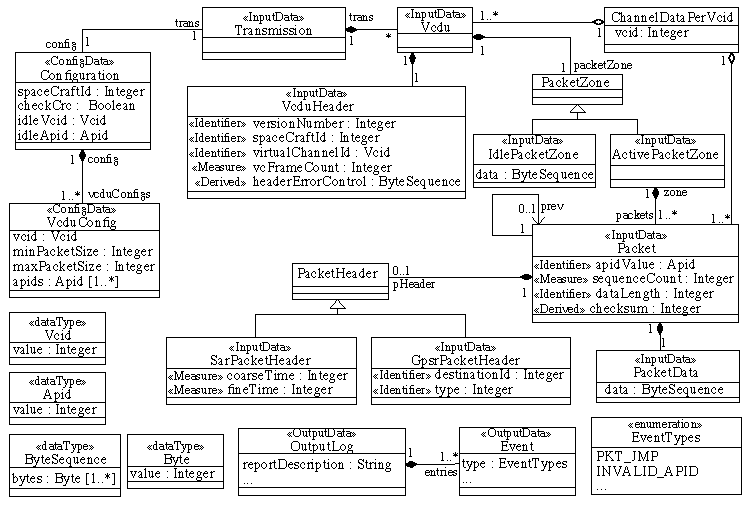
\includegraphics{images/classDiagramSmall}
%      \caption{Simplified input data model taken from~\cite{di2015evolutionary}.}
%      \label{fig:dataModel}
%\end{figure}
%
%\begin{figure}[h]
%  \centering
%    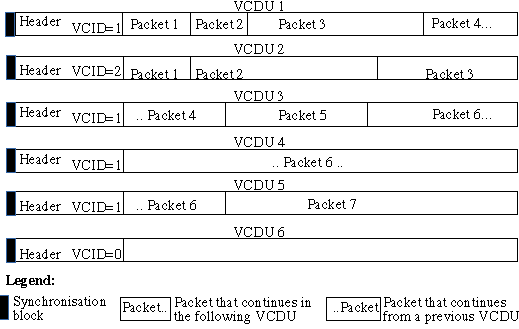
\includegraphics{images/transmissionData}
%      \caption{A simplified example of the transmission data modelled by the class diagram in Figure~\ref{fig:dataModel}.}
%      \label{fig:transmissionData}
%\end{figure}
%
%\begin{figure}[h]
%  \centering
%    \includegraphics{images/CADU}
%      \caption{Header of VCDU 3 followed by a portion of its packet zone.}
%      \label{fig:VCDU}
%\end{figure}
%
%\begin{figure}[h]
%  \centering
%    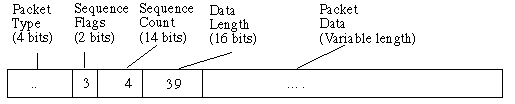
\includegraphics{images/packet}
%      \caption{Structure of a packet.}
%      \label{fig:packet}
%\end{figure}
%
%
%
%
%% An example fault model is described in Table~\ref{table:faultModel:SES}.
%%%and are used to identify the fields that can be mutated to generate new inputs.
%%For example, 
%%the two stereotypes \emph{Identifier} and \emph{Measure} are used to indicate that these attributes should be modified using mutation operators specified for identifiers and measurements.
%
%
%In the presence of UML models, constraints between inputs and outputs can be represented using OCL.
%These constraints are used as an oracle to validate the execution of automatically generated test cases: a violated constraint indicates that the system under test does not produce the expected output. 
%%The use of OCL constraints enable engineers to represent information that cannot be captured with grammars.
%%In the case of SES-DAQ, we use OCL constraints to model the error messages expected in the presence of specific faults in the input data.
%For example, Figure~\ref{fig:costraint:firstHeader} shows an OCL constraint that states that the frame count of a VCDU should be greater by one than the frame count of the previous VCDU on the same virtual channel. Otherwise, an error event \emph{COUNTER\_JUMP} should exist in the system output log file. 
%In the context of data-driven mutation testing they can be used to determine if a mutant had been killed by a test case (e.g., a constraint may capture the presence of a log entry indicting the triggering a redundancy mechanism).
%
%
%
%\begin{figure}[t!]
%\scriptsize
%\begin{tabular}{p{0.1cm}p{8cm}}
%1&\textbf{context} Vcdu \textbf{inv}:\\
%2&\textbf{let}\\
%3&\hspace{0.3cm}frameCount : Integer = self.header.vcFrameCount, \\
%4&\hspace{0.3cm}vdcuIndex : Integer = self.virtualChannel.vcdu$\rightarrow$indexOf( self ), \\
%5&\hspace{0.3cm}previous : Vcdu = self.virtualChannel.vcdu$\rightarrow$at( vcduIndex - 1 ),\\
%6&\hspace{0.3cm}previousFrameCount : Integer = previous.header.vcFrameCount\\
%7&\textbf{in} \\
%8&\hspace{0.3cm}\textbf{if} previousFrameCount $<$ 16777215 \\
%9&\hspace{0.6cm}\textbf{then} frameCount $<>$ previousFrameCount + 1 \\
%10&\hspace{0.3cm}\textbf{else} previousFrameCount $=$ 16777215 and frameCount $<>$ 0 \textbf{endif}\\
%11&\textbf{implies} \\
%12&\hspace{0.3cm}VcduEvents.allInstances()\\
%13&\hspace{1cm}$\rightarrow$exists(e $|$ e.eventType = $COUNTER\_JUMP$) \\
%\end{tabular}
%\caption{Input/output constraint for the \emph{COUNTER\_JUMP} error event.}
%\label{fig:costraint:firstHeader}
%\end{figure}
%
%
% 
%%The stereotype \emph{Derived} is used to tag class attributes that need to be derived from other attributes after every mutation, in order to prevent trivial inconsistencies (e.g. it is used to update the checksum field when other fields are mutated). 
%%The stereotypes \emph{StreamClass} and \emph{StreamAttributes} are used to automate the loading of data from bytestreams.
%% but are out of the scope of this paper (see~\cite{ICST15} for details).
%
%The main limitation of UML-based approaches is the lack of generalistic binary parsers capable of loading data as an instance of a UML class diagram. Existing approaches rely on custom parsers~\cite{di2015generating,di2015evolutionary}.
%
%\subsubsection{Data modeling with Block Models}
%
%Approaches relying on block models~\cite{PeachFuzzer,spike,pham2016model}, require that engineers specify input data according to a specific format that captures the size of specific portions of the input data. 
%For example, Spike~\cite{spike} and Peach~\cite{PeachFuzzer} require input models that specify the format of data chunks and integrity constraints.
%Figure~\ref{fig:pit} shows a portion of an example block model taken from related work~\cite{pham2016model}.
%While being effective in fuzzing programs that process weakly-structured inputs (e.g., images and protocols), these approaches become less effective for highly-structured inputs (e.g., JavaScript).
%Compared to UML-based modeling, block models provide more limited modeling capabilities, for instance, they are less effective for highly-structured inputs; however, they are often integrated into general-purpose tools that can be easily integrated in software projects~\cite{PeachFuzzer}.
%
%
%\begin{figure}[t!]
%  \centering
%    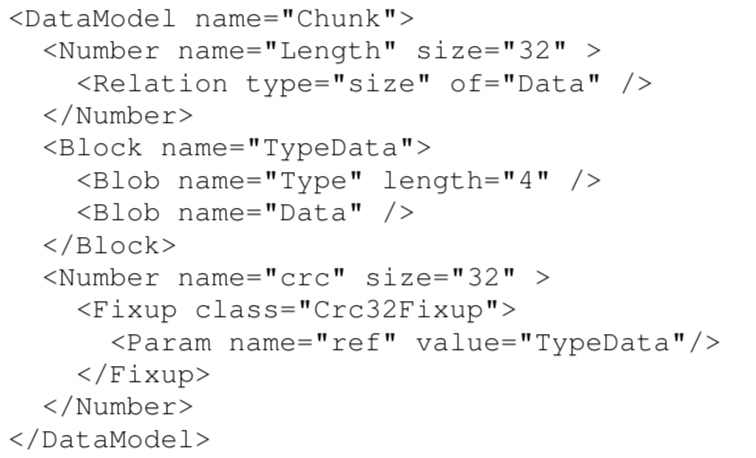
\includegraphics[width=7cm]{images/PeachPit}
%      \caption{Data model with a custom format.}
%      \label{fig:pit}
%\end{figure}
%
%
%%%%%%%%%%%%%%%%%%%%%%%%%%%%%%%%%%
%
%\subsection{Data-driven Mutation Operators}
%\label{sec:data_operators}
%
%%As mentioned in Section~\ref{sec:dataProcess}, the software engineering literature does not include any study on data-driven mutation testing but only testing approaches based on the injection of data faults.
%%For this reason, 
%In this section, we provide an overview of the fault injection techniques that have originally been developed to support software testing and can be used in the context of data-driven mutation testing. 
%More precisely, we focus on the techniques for the modification of data (hereafter, data mutation techniques) that are presented in software testing research papers.
%
%
%Table~\ref{table:dataOperators} provides an overview of groups of data mutation techniques that can be applied to space software and embedded systems. 
%We selected the set of data-driven mutation techniques in Table~\ref{table:dataOperators} based on the different types of faults commonly affecting space and embedded systems.
%Each technique aims to create data faults that might be observed in real systems either because of hardware errors or software errors.
%The data-driven mutation operators, i.e., the specific functions implemented by each technique to alter the type of data they target, are described in separate tables, in the following paragraphs. 
%%Since, for each family of technique, multiple implementations of data-driven mutation operators are available
%
%In Table~\ref{table:dataOperators}, column \emph{Name} provides the name of the specific technique described,  
% column \emph{Type of fault} indicates the type of faults each operator aims to simulate,
% column \emph{Data model} indicates if the technique requires a model of the structure of the data to be mutated,
% column \emph{Definition} provides a brief description of the technique, column \emph{Target} indicates the type of data targeted,
% column \emph{Reference} provides a reference to a research paper or tool describing the technique more in detail.
% 
%%Fabrizio: "First" and "Then" read like a story, which is not good in a Tech Report
%Concerning the type of faults considered, we focus both on hardware and software errors.
%Hardware errors are captured by the categories CPU Faults, Memory Faults, and Signal Faults. 
%Software errors are captured by the category Data Processing Faults.
%Category Communication Faults simulates problems that can be caused either by software or hardware errors.
%
%
%
%\newcommand{\FTAPE}{\cite{tsai1999stress}}
%\newcommand{\FIAT}{\cite{barton1990fault}}
%\newcommand{\GOOFI}{\cite{aidemark2001goofi}}
%\newcommand{\DOCTOR}{\cite{han1995doctor}}
%\newcommand{\ORCHESTRA}{\cite{dawson1996testing}}
%\newcommand{\Fuzz}{\cite{miller1995fuzz}}
%\newcommand{\Ballista}{\cite{koopman2000exception}}
%\newcommand{\RIDDLE}{\cite{ghosh1998testing}}
%\newcommand{\Superion}{\cite{Wang:GrammarAwareFuzzying:ICSE:2019}}
%\newcommand{\AFL}{\cite{gutmann2016fuzzing}}
%\newcommand{\SAGE}{\cite{godefroid2012sage}}
%\newcommand{\pFuzzer}{\cite{mathis2019parser}} 
%\newcommand{\MoWF}{\cite{pham2016model}}
%\newcommand{\DiNardoICST}{\cite{di2015generating}}
%\newcommand{\DiNardoASE}{\cite{di2015evolutionary}}
%\newcommand{\Matinnejad}{\cite{Matinnejad19}}
%\newcommand{\MongoDB}{\cite{Guo:MongoDBFuzzer:CACM:2017}}
%\newcommand{\SOLMI}{\cite{Jan:ISSTA:2016}}
%\newcommand{\MUSQL}{\cite{Appelt:SQLI:ISSTA:2014}}
%
%Table~\ref{table:dataMutation:references} provides the names of the tools and approaches referenced in Table~\ref{table:dataOperators}, along with a URL for the download of the tool, if available.
%
%% !TEX root =  ../MutationTestingSurvey.tex

\begin{table}[ht]
\tiny
\caption{Description of approaches and tools appearing in Table~\ref{table:dataOperators}.}
\begin{center}
\begin{tabular}{|p{1cm}|p{4cm}|p{8cm}|}
\hline
\textbf{Reference} & \textbf{Approach and Tool name} & \textbf{Available} \\
\hline

\cite{di2015evolutionary}	& Di Nardo et al. Search-based Mutation & No \\
\cite{di2015generating} & Di Nardo et al. Model-based Mutation & No \\
\cite{Matinnejad19} & Matinnejad et al. Signal Mutation & No \\

\cite{tsai1999stress} & FTAPE & No\\
\cite{barton1990fault} & FIAT & No \\
\cite{han1995doctor} & DOCTOR & No \\
\cite{dawson1996testing} & ORCHESTRA & No \\

\cite{miller1995fuzz} & Fuzz & Yes, \url{http://pages.cs.wisc.edu/~bart/fuzz/fuzz.html} \\


\cite{koopman2000exception}	&  Ballista & Yes, \url{http://users.ece.cmu.edu/~koopman/ballista/} \\

%\cite{ghosh1998testing}	& RIDDLE & No \\
\cite{Wang:GrammarAwareFuzzying:ICSE:2019} & Superion & \url{https://github.com/zhunki/Superion} \\
\MongoDB	& MongoDB Fuzzer & No \\
\SOLMI	& SOLMI &No \\
\MUSQL	& \emph{$\mu$4SQLi} &No\\
\cite{gutmann2016fuzzing} & American Fuzzy Lop & Yes, \url{https://github.com/google/AFL}\\
\cite{godefroid2012sage} & SAGE & \begin{tabular}[c]{@{}l@{}}Yes, now under Microsoft Security Risk Detection service\\\url{https://www.microsoft.com/en-us/security-risk-detection/}\end{tabular} \\
%\cite{mathis2019parser}	& pFuzzer & Yes, \url{https://github.com/uds-se/pFuzzer}\\
\cite{pham2016model} &	MoWF & No \\
\cite{spike}&SPIKE&\url{https://github.com/guilhermeferreira/spikepp}\\
\cite{PeachFuzzer}&PEACH&\url{https://www.peach.tech}\\
\cite{BooFuzz}&BooFuzz&\url{https://github.com/jtpereyda/boofuzz}\\
\hline
\end{tabular}
\end{center}
\label{table:dataMutation:references}
\end{table}%


%
%% !TEX root =  ../MutationTestingSurvey.tex

\newcommand{\FTAPE}{\cite{tsai1999stress}}
\newcommand{\FIAT}{\cite{barton1990fault}}
\newcommand{\GOOFI}{\cite{aidemark2001goofi}}
\newcommand{\DOCTOR}{\cite{han1995doctor}}
\newcommand{\ORCHESTRA}{\cite{dawson1996testing}}
\newcommand{\Fuzz}{\cite{miller1995fuzz}}
\newcommand{\Ballista}{\cite{koopman2000exception}}
\newcommand{\RIDDLE}{\cite{ghosh1998testing}}
\newcommand{\AFL}{\cite{gutmann2016fuzzing}}
\newcommand{\SAGE}{\cite{godefroid2012sage}}
\newcommand{\pFuzzer}{\cite{mathis2019parser}} 
\newcommand{\MoWF}{\cite{pham2016model}}
\newcommand{\DiNardoICST}{\cite{di2015generating}}
\newcommand{\DiNardoASE}{\cite{di2015evolutionary}}
\newcommand{\Matinnejad}{\cite{Matinnejad19}}

\begin{itemize}
	\item FTAPE tool: \cite{tsai1999stress}
	\item FIAT tool: \cite{barton1990fault}
	\item GOOFI tool: \cite{aidemark2001goofi}
	\item DOCTOR tool: \cite{han1995doctor}
	\item ORCHESTRA tool: \cite{dawson1996testing}
	\item Fuzz tool:\cite{miller1995fuzz}
	\item Ballista tool: \cite{koopman2000exception}
	\item RIDDLE tool: \cite{ghosh1998testing}
	\item American Fuzzy Lop tool: \cite{gutmann2016fuzzing}
	\item SAGE tool: \cite{godefroid2012sage}
	\item pFuzzer tool: \cite{mathis2019parser}
	\item MoWF tool: \cite{pham2016model}
	\item Di Nardo et al. Model-based Mutation tool: \cite{di2015generating}
	\item Di Nardo et al. Search-based Mutation tool: \cite{di2015evolutionary}
	\item Matinnejad et al. Signal Mutation tool: \cite{Matinnejad19}
\end{itemize}

\tiny
\setlength\LTleft{0pt}
\setlength\LTright{0pt}
\begin{longtable}{@{\extracolsep{\fill}}|p{1.5cm}|p{2cm}|p{5cm}|p{3cm}|p{1cm}|@{}}
\toprule
	\textbf{Name}	&	\textbf{Type of Fault}	&	\textbf{Definition}	&	\textbf{Target}	&	\textbf{Reference} \\
	\midrule
stuck-at-0 & CPU Faults; Memory Faults & This operator corrupts data by replacing a bit/byte/word with zero. & CPU registers; Memory registers & \FTAPE, \FIAT, \GOOFI \\
stuck-at-1 & CPU Faults; Memory Faults & This operator corrupts data by replacing a bit/byte/word with one. & CPU registers; Memory registers & \FTAPE, \FIAT, \GOOFI \\
bit flips & CPU Faults; Memory Faults; Data Processing Faults & This operator mutates data by inverting the value of each bit (i.e., replacing 0 with 1 and 1 with 0). & CPU registers: saved registers, floating point registers, the program counter, global pointer, stack pointer; Local memory; Input or output parameters of a software interface. & \FTAPE, \FIAT, \GOOFI \\
disk driver codes & Communication Faults & This operator performs data mutation by modifying the error flags of a disk driver. & I/O disk driver codes. & \FTAPE \\
set & CPU Faults; Communication Faults; Memory Faults & This operator sets the value of a bit/byte by replacing the current value with one or a user-defined bitmap. & Memory: stack, heap, global data, user code, user-defined memory location; Registers: data, stack, address, program counter, status register & \FTAPE, \FIAT, \GOOFI \\
clear & CPU Faults; Communication Faults; Memory Faults & This operator clears the value of a bit/byte by replacing the current value "v" with zero. & Memory: stack, heap, global data, user code, kernel code, user-defined memory location; Registers: data, stack, address, program counter, status register & \FTAPE, \FIAT, \GOOFI \\
toggle & CPU Faults; Communication Faults; Memory Faults & This operator toggles (i.e., sets a bit to its complement state) a bit/byte. & Memory: stack, heap, global data, user code, kernel code, user-defined memory location; Registers: data, stack, address, program counter, status register & \FTAPE, \FIAT, \GOOFI \\
lose message & Communication Faults & This operator causes a message to be lost in between two communicating components. Messages can be lost intermittently, with a probability distribution specified by the users, or alternatively, every message can be lost during a certain period. & Faulty link, Faulty direction, Single message & \DOCTOR, \ORCHESTRA \\
duplicate message & Communication Faults & This operator causes a message to be duplicated in between two communicating components. & Faulty link, Faulty direction, Single message & \DOCTOR, \ORCHESTRA \\
alter message header & Communication Faults & This operator alters a message. The change is performed in a similar manner as for memory faults, i.e., by performing bit flips. The mutation is performed in the message header. & Faulty link, Faulty direction, Single message & \DOCTOR, \ORCHESTRA \\
alter message body & Communication Faults & This operator alters a message. The change is performed in a similar manner as for memory faults, i.e., by performing bit flips. The mutation is performed in the message body. & Faulty link, Faulty direction, Single message & \DOCTOR, \ORCHESTRA \\
delay message & Communication Faults & This operator causes a message to be delayed in between two communicating components. The delay time can either be constant or follow a probability distribution. & Faulty link, Faulty direction, Single message & \DOCTOR, \ORCHESTRA \\
fuzzing & Data Processing Faults & Fuzzing techniques replace values with values (i.e., fuzz values) that are different and, usually, randomly generated. & Structured input data (e.g., files, streams) & \Fuzz, \Ballista \\
grammar-based fuzzing & Data Processing Faults & This fuzzing approach relies on a grammar that describes the format of the data to be altered; new values are generated according to the grammar. The use of the grammar decreases the chances of generating invalid inputs. & Structured input data (e.g., files, streams) & \RIDDLE \\
evolutionary fuzzing & Data Processing Faults & This fuzzing approach relies on evolutionary algorithms (e.g., genetic algorithms) to generate fuzz values. It relies on a fitness function to maximize structural coverage (e.g., branches executed during testing). The fitness is implemented by instrumenting the code of the application to collect code coverage. & Structured input data (e.g., files, streams) & \AFL \\
whitebox fuzzing & Data Processing Faults & This fuzzing approach relies on symbolic execution techniques to cover corners cases on the different execution paths. & Structured input data (e.g., files, streams) & \SAGE \\
parser-directed fuzzing & Data Processing Faults & Fuzzing techniques replace a correct value with a randomly generated one. This fuzzing operator is applied to programs that integrate a parser component to extract information from the provided inputs. It is implemented through a test generator technique that aims to produce valid inputs for the parser, the inputs are produced randomly and then checked using constraint solving techniques. & Structured input data (e.g., files, streams) & \pFuzzer \\
model-based whitebox fuzzing & Data Processing Faults & Fuzzing techniques replace a correct value with a randomly generated one, in this case, the replacement is done using a model-based whitebox fuzzing technique, the technique prunes from the search space those paths that are exercised by invalid, malformed inputs. The model should specify the format of the data chunks and integrity constraints. & Structured input data (e.g., files, streams) & \MoWF \\
data-type based injection & Data Processing Faults & This operator replaces a value with an invalid one, selected on the basis of the type of the parameter being corrupted. & Structured input data (e.g., files, streams) & \Fuzz, \Ballista, \RIDDLE \\
model-based mutation & Data Processing Faults & This approach alters existing inputs by relying on a data model that capture the structure of the data and the constraints among data fields. A predefined set of operators indicating how to alter data based on its structure are provided. & Structured input data (e.g., files, streams) & \DiNardoICST \\
search-based data mutation & Data Processing Faults & This approach alters existing inputs by relying on a data model that captures the structure of the data and the constraints between data fields. A search-based, evolutionary algorithm is used to maximize a number of mutation objectives including the number of constraints being violated and code coverage. & Structured input data (e.g., files, streams) & \DiNardoASE \\
signal mutation & Signal faults & This approach alters signal by either shifting the signal based on a randomly selected value or shifting the signal and increasing the number of signal pieces (i.e., segments).  & Input signals & \Matinnejad \\

	\bottomrule                                                             
\caption{Data-driven Mutation Operators.}
\label{table:dataOperators}
\end{longtable}
\normalsize
%
%To summarize the data in Table~\ref{table:dataOperators}, we observe that:
%\begin{itemize}
%  %Note: always put a comma at the end of a list before "or" "and"
%  \item Category CPU Faults includes techniques that perform mutations in the contents of an individual bit, byte, or word in a CPU register. The mutations in this category can target saved, floating-point, program-counter, global and stack-pointer register locations. 
%  \item Category Memory Faults includes techniques that perform mutations in the contents of an individual bit, byte, or word in a memory register. The mutations in this category can target stack, heap, global-data and user-defined memory locations.
%  \item Category Communication Faults includes techniques that simulate packet corruption faults. The mutations in this category can target channels between components, single messages, and the addresses of the messages to be exchanged.
%  \item Category Data Processing Faults includes techniques that mutate the data being processed by the system. Some of these techniques are white-box, they process the source code of the application to generate inputs more efficiently. Other techniques require a model of the data to be mutated. The mutations in this category can target both the input and the output parameters of the interface of a software component.
%  \item Category Signal Faults includes techniques that alter the shape of the signals received by the software under test.
%\end{itemize}
%
%In the following, we provide an overview of the mutation operators implemented by the most representative techniques.
%We do not present simple fuzzing approaches because they simply perform random mutations and they include a subset of the operators implemented in the more advanced evolutionary fuzzing approaches.
%
%\subsubsection{Blind memory corruption and blind transmission corruption}
%
%The mutation operators implemented by techniques performing blind memory corruption and blind transmission corruption are presented in Tables~\ref{table:operators:blindTransmissions} and ~\ref{table:operators:blindTransmissions}, respectively. These techniques do not require a data model. Unfortunately, they are of little usefulness to simulate subtle errors that affect relations among data (e.g., replacing an identifier with another legal one).
%
%%Among all the data mutation operators reported in Table~\ref{table:dataOperators}, the ones targeting \emph{Data Processing Faults} are more powerful since they concern the modification of complex data structures. %Oscar: not sure that "overviewed" is spelled right %They are briefly overviewed in the following.
%%We provide an overview in the following.
%
%
%\subsubsection{Evolutionary Fuzzing}
%
%
%%\subsubsection{Approaches generating data from scratch}
%AFL is an instrumentation-guided fuzzer~\cite{gutmann2016fuzzing}. It integrates genetic algorithms with a form of branch coverage called state transition coverage,
%which captures the number of times each branch is taken in an execution. 
%AFL aims to generate inputs that exercise all the different code paths.
%%It is implemented by executing for every instruction of the program under test the following lines
%%cur_location = <COMPILE_TIME_RANDOM>;
%%coverage[cur_location ^ prev_location]++; 
%%prev_location = cur_location >> 1;
%It requires one or more starting files that contain input data normally processed by the targeted application. 
%Each provided input is processed in a queue. For each input in the queue, AFL trims the test case to the smallest size that doesn't alter the coverage of the program. Then it repeatedly mutates the file using a set of fuzzing strategies, which are presented in Table~\ref{table:AFL:operators}.
%If any of the generated mutations result in a change of the coverage for the software under test, the mutated input is added to the input queue.
%
%% !TEX root =  ../MutationTestingSurvey.tex

%
%\setlength\LTleft{0pt}
%\setlength\LTright{0pt}
%\begin{longtable}{@{\extracolsep{\fill}}|p{2.5cm}|p{5cm}|p{5cm}|@{}}
%\toprule


\begin{table}[h]
\caption{Mutation Operations performed by AFL~\cite{gutmann2016fuzzing}}
\label{table:AFL:operators}


\tiny
\begin{tabular}{|p{2.5cm}|p{10cm}|}

\hline

\textbf{Walking bit flips}& Sequential, ordered bit flips. The number of bits flipped in a row varies from one to four in steps of two. This strategy is applied till the coverage of the program under test does not change.\\

\hline
\textbf{Walking byte flips}& This method relies on 8-, 16-, or 32-bit wide bitflips with a constant stepover of one byte. \\

\hline
\textbf{Simple arithmetics}& Increment and decrement existing integer values in the input file; this is done considering every byte of the file. The chosen range for the operation is -35 to +35. It is performed in three steps. First, the fuzzer attempts to perform subtraction and addition on individual bytes. The second steps involves looking at 16-bit values, using both endians - but incrementing or decrementing them only if the operation has affected the most significant byte. The final stage follows the same logic, but for 32-bit integers.\\

\hline
\textbf{Known integers}& 
AFL overwrites every byte in the input file with a set of interesting values (e.g., -1, 256, 1024, MAX\_INT-1, MAX\_INT), using both endians (the writes are 8-, 16-, and 32-bit wide).\\

\hline
\textbf{Stacked tweaks}& Sequence of randomly selected mutations among the following: Single-bit flips, Attempts to set "interesting" bytes, words, or dwords (both endians), Addition or subtraction of small integers considering bytes, words, or double words (both endians), Random single-byte sets, Block deletion, Block duplication via overwrite or insertion, Block memset. \\

\hline
\textbf{Test case splicing}& Consists of taking two distinct input files that differ in at least two locations, splicing them at a random location in the middle, and then applying stacked tweaks.\\

\hline
%\bottomrule                                                             

\end{tabular}
\end{table}
%\normalsize



%
%\subsubsection{Grammar-based fuzzing}
%
%Superion~\Superion~ extends \emph{AFL} to drive mutations based on grammars. It takes as input an ANTLR~\cite{ANTLR} grammar. 
%It performs mutations that consist of grammar-aware trimming, dictionary-based mutations, and tree-based mutation.
%Grammar-aware trimming is performed by generating an AST tree from the input and by deleting a randomly-selected subtree. 
%It aims to generate trimmed inputs that do not alter code coverage in the SUT.
%Dictionary-based mutations are performed by building a dictionary using every token in the input file and by inserting the elements of the dictionary in the boundaries of every token in the input file.
%Tree-based mutation is performed by processing two input files and replacing the subtrees of one file with the ones of another.
%Listing~\ref{mutatedJSONfile} shows a JSON file generated by deleting a randomly-selected subtree from Listing~\ref{JSONfile}.
%
%
\begin{minipage}{14cm}
\footnotesize
\begin{lstlisting}[caption=JSON file generated by deleting a subtree from Listing~\ref{JSONfile}., label=mutatedJSONfile]
{
 [
 {
  "firstName": "Fabrizio",
  "lastName": "Pastore",
  "isAlive": true,
  },
  {
  "firstName": "Oscar",
  "lastName": "Cornejo",
  "isAlive": true,
  "address": {
    "streetAddress": "29, Avenue J.F Kennedy",
    "city": "Luxembourg",
    "state": "Luxembourg",
    "postalCode": "L-1855"
  },
  }
  ]
}
\end{lstlisting}
\end{minipage}
%
%%Fabrizio: you had this definition of equivalent: "(i.e., correct fuzzed data, but semantically meaningless)." it is difficult to understand
%
%
%%Fabrizio: I cannot understand the following sentences
%%Although it tackles the problem of redundant mutants by well covering the space of possible inputs, it does not tackle the redundant mutant problem.
%%Cannot handle semantic restrictions imposed by certain nontrivial input languages. The approach has difficulties to handle complex sequences recursion.
%
%%\subsubsection{Approaches altering existing data}
%
%
%\emph{$\mu$4SQLi}~\cite{Appelt:SQLI:ISSTA:2014} relies on a SQL grammar to generate SQL injections. 
%SQL injections are generated by means of a set of mutation operators, shown in Table~\ref{table:Mu4SQLI}, that alter the values of an input according to predefined patterns.
%Similarly, SOLMI~\cite{Jan:ISSTA:2016} relies on the XML grammar to alter XML messages based on a predefined set of mutation operators and introduce potential XML injections. 
%SOLMI implements four operators that (1) introduce XML meta-characters, (2) introduce closing tags, (3) replicate XML elements, (4) replace XML content.
%
%
%\begin{table}[h]
%\caption{Mutation operators implemented by $\mu$4SQLi}
%\label{table:Mu4SQLI}
%\begin{tabular}{|p{2cm}|p{11.5cm}|}
%\hline
%\multicolumn{2}{|c|}{Behaviour-Changing Operators}\\
%\hline
%MO\_or&Adds an OR-clause to the input\\
%MO\_and&Adds an AND-clause to the input\\
%MO\_semi&Adds a semicolon followed by an additional SQL statement\\
%\hline
%\multicolumn{2}{|c|}{Syntax-Repairing Operators}\\
%\hline
%MO\_par&Appends a parenthesis to a valid input\\
%MO\_cmt&Adds a comment command (- - or \#) to an input\\
%MO\_qot&Adds a single or double quote to an input\\
%\hline
%\multicolumn{2}{|c|}{Obfuscation Operators}\\
%\hline
%MO\_wsp&Changes the encoding of whitespaces \\
%MO\_chr&Changes the encoding of a character literal enclosed in quotes\\
%MO\_html&Changes the encoding of an input to HTML entity encoding\\
%MO\_per&Changes the encoding of an input to percentage encoding\\
%MO\_bool&Rewrites a boolean expression while preserving its truth value\\
%MO\_keyw&Obfuscates SQL keywords by randomising the capitalisation and inserting comments\\
%\hline
%\end{tabular}
%\end{table}
%
%
%Tal et al.~\cite{Tal2004} presented a syntax-based vulnerability testing technique based on mutations of ASN.1 grammars. The objective is to detect software vulnerabilities detecting anomalous behavior or crashes in the SUT (e.g., segmentation faults, buffer, heap or stack overflows, etc.) when parsing mutated PDUs. The PDUs are specified by frames (data structures), which explicitly defines the order of data fields in the PDU, as well as the exact length of each field. 
%The proposed approach intercepts OSPF packets and translates it to a TXL readable file, then the mutations are applied to ASN.1 syntax contained in the TXL file. The mutation strategies applied are the following: \textbf{replacement} (replacing one field at a time with boundary and mid-way values), \textbf{removal} (removing one field at a time, and then removing pairs of fields, one pair at a time), and \textbf{permutation} (permutating pairs of fields within each SEQUENCE and SET).
%
%% \textbf{Syntax-based Vulnerability Testing of Frame-based Network Protocols}
%% \cite{Tal2004} The paper presents a syntax-based vulnerability testing technique based on mutations of Protocol Data Units (PDU) performed on the ASN.1 syntax. The objective is to detect software vulnerabilities detecting anomalous behavior or crashes in the SUT (e.g., segmentation faults, buffer, heap or stack overflows, etc.) when parsing mutated PDUs. The PDUs are specified by frames (data structures), which explicitly defines the order of data fields in the PDU, as well as the exact length of each field.
%% Syntax is specified in BNF notation, mutations are then made to the syntactic elements and the grammar is used to produce mutated vectors (PDUs). In the paper, the transferred packets are based on the OSPF protocol. Previously, it has been applied to WAP, HTTP, LDAP and SNMP protocols.
%% The proposed approach intercepts a packet and translates it to a TXL readable file, then the mutations are applied to ASN.1 syntax contained in the TXL file. The mutation strategies applied are the following: replacement (replacing one field at a time with boundary and mid-way values), removal (removing one field at a time, and then removing pairs of fields, one pair at a time), and permutation (permutating pairs of fields within each SEQUENCE and SET).
%
%
%% \textbf{CMM: A combination-based mutation method for SQL injection}
%
%Instead, Zhao et al.~\cite{Zhao2020} presented a mutation-based fuzzing technique for eliminating SQLi vulnerabilities. The technique is called Combinatorial Mutation Method (CMM), which mixes combinatorial testing with fuzzing techniques to generate test sets for SQLi. 
%
%The mutations are based on the mutation methods from sqlmap (open source penetration testing tool that automates the process of detecting and exploiting SQLi flaws). The authors classifies the mutation methods provided by sqlmap in five groups:
%
%
%\begin{table}[h!]
%\begin{center}
%\begin{tabular}{|p{2cm}|p{10cm}|}
%\hline
%\textbf{Fault}&\textbf{Description}\\
%\hline
%comment & attach a sql comment command at the back of an input test case.\\
%stringtamper & changes the appearance of an input, making it look valid but still malicious. \\
%space2 & changes the space character in the input.\\
%apostle& changes the apostle in the input.\\
%encoding& this kind of mutation method changes the encoding of the original statement.\\
%\hline
%\end{tabular}
%\end{center}
%\caption{Fault Model from \cite{Zhao2020}}
%\label{table:faultModel:Zhao2020}
%\end{table}%
%
%The test set is created by using combinatorial testing on the different inputs created by the mutation tool.
%
%
%
%%\textbf{Testing for software vulnerability using environment perturbation}
%
%Du et al.~\cite{Du2002} introduced a fault injection technique to perform environment perturbations for testing a software system for possible security flaws. The paper introduces a fault model called Environment-Application Interaction (EAI).
%
%Given the assumption that a system is composed of an application plus its environment, in the paper faults are injected into the environment thereby perturbing it, the idea is to verify if the program responds and whether there will be a security violation under this perturbation, otherwise the system is considered secure.
%
%The faults are injected at the points where the environment and the application interact. The environment faults becomes faults in the input, which is then inherited by an internal entity of the application. From this point onwards the environment faults propagate through the application via the internal entities. If the application does not handle the faults correctly, a security violation might occur. The direct reason for this violation appears to be faults in the internal entity. 
%Authors classify environment faults in two categories: (1) indirect: affect programs via internal entities (primary sources of program inputs). (2) direct: affect programs via environment faults.
%
%
%\begin{figure}[h]
%  \centering
%    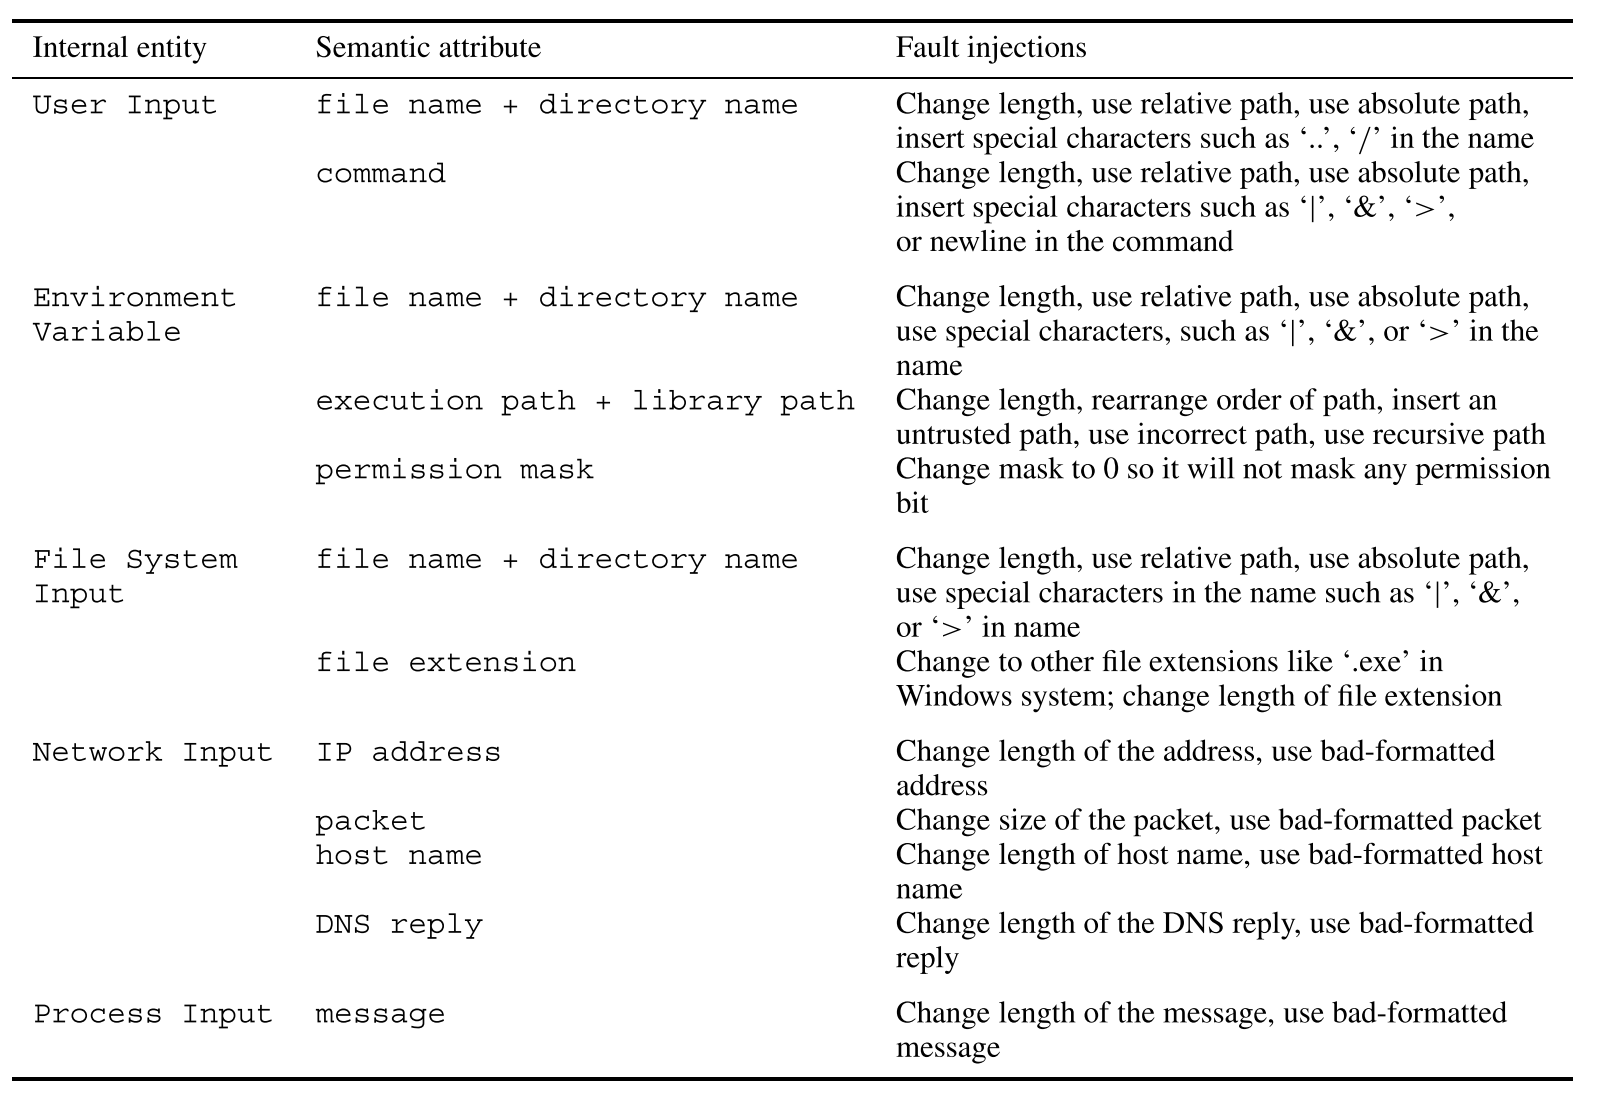
\includegraphics[width=0.8\textwidth]{images/du2002a}
%      \caption{Indirect environment faults and environment perturbations operators.}
%\end{figure}
%
%
%\begin{figure}[h]
%  \centering
%    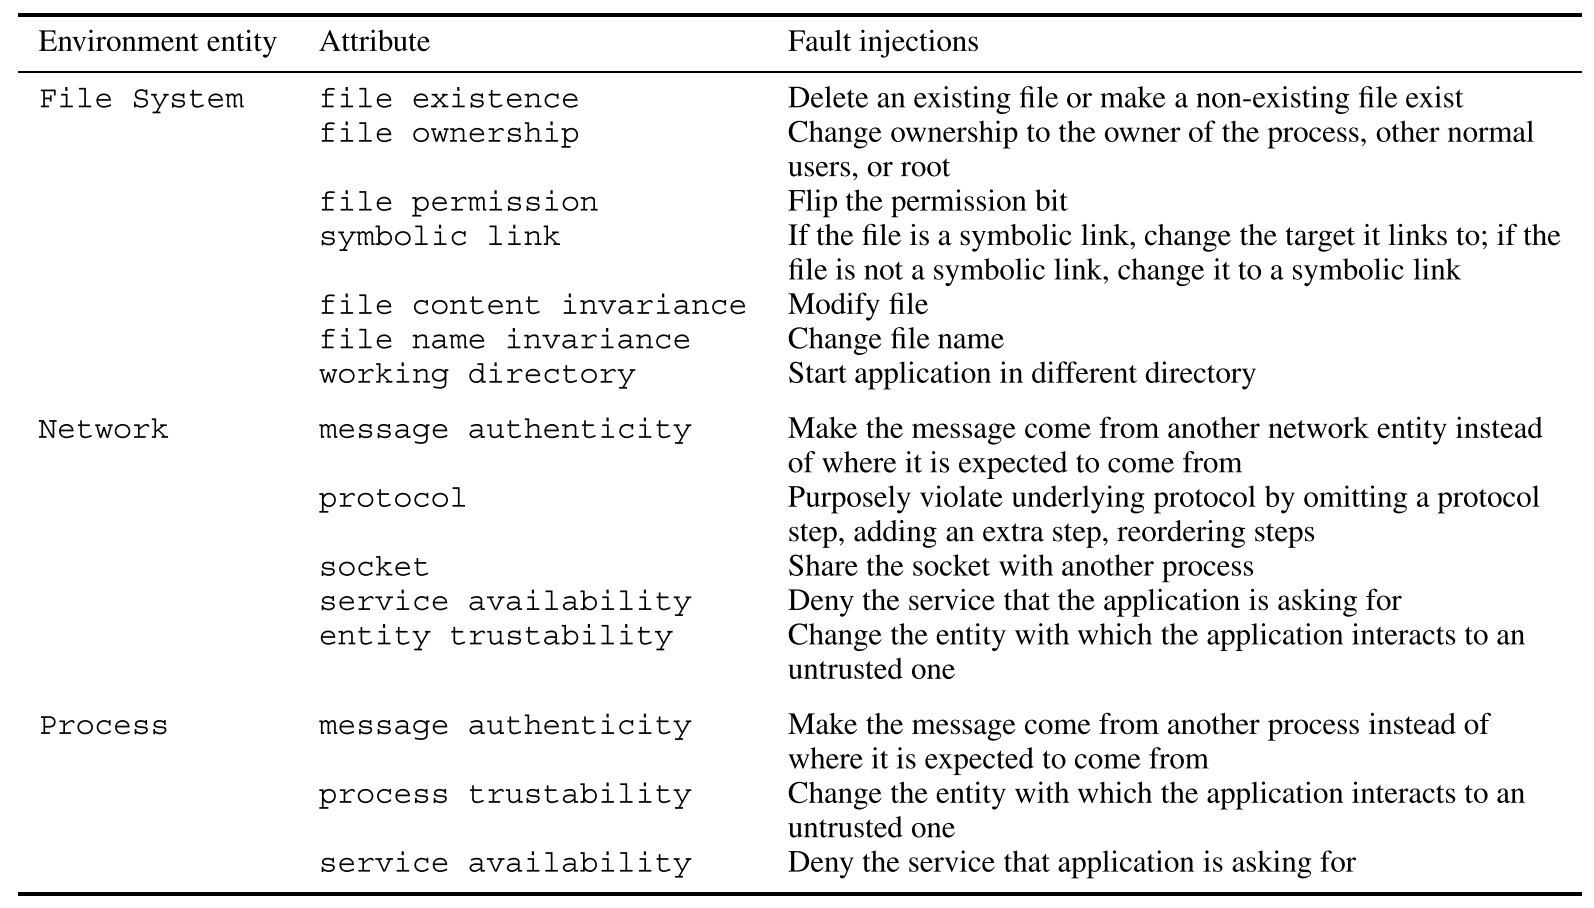
\includegraphics[width=0.8\textwidth]{images/du2002b}
%      \caption{direct environment and environment perturbations operators.}
%\end{figure}
%
%They use fault coverage (percentage of the number of faults tolerated to the faults injected) and interaction coverage (percentage of the number of interaction points where faults are injected w.r.t to total of interaction points) to measure the test adequacy.
%
%
%
%One of the major limitations of grammar-based approaches is the cost of defining an input grammar. MongoDB's javascript fuzzer addresses the problem of grammar-based mutation when a grammar is not available. Instead of mutating input files for the SUT based on the input grammar of  the SUT, it mutates test cases for the SUT (in this case the Javascript test cases)~\MongoDB. It replaces subtrees in the AST tree generated from the test cases either other subtrees belonging to the same input file or with subtrees generated following encoded production rules.
%
%
%
%
%
%\subsubsection{Whitebox fuzzing}
%
%%, also, it requires more knowledge about the target than purely random ones.
%
%SAGE adopts symbolic execution to systematically generate malformed inputs~\cite{godefroid2012sage}. SAGE performs fuzzing on file- and packet-parsing applications. 
%The program is first executed with concrete inputs; in order to identify a set of constraints on inputs, then, one of the constraints in the set is negated, and new malformed inputs are generated to satisfy the new set of constraints. 
%The main benefit of SAGE is that it forces the program to execute corner cases not covered by the initial inputs; for example, 
%%Fabrizio: you wrote the following, which I could not understand please check if my sentence is correct
%%(e.g., reached one-third of all bugs found by fuzz testing in Microsoft projects \cite{bounimova2013billions}).
%%Oscar: yes, what you wrote is correct 
%one-third of all the bugs found by means of fuzz testing are detected thanks to SAGE \cite{bounimova2013billions}.
%Unfortunately, the main limitation of SAGE and symbolic execution-based fuzzers is its limited scalability, due to the high execution time required by symbolic execution.
%
%%Fabrizio: not sure what the following is about, ignoring
%%\emph{Testing of Fault-Tolerant and Real-Time Distributed Systems via Protocol Fault Injection \cite{dawson1996testing}}: The paper introduces a portable fault injection environment for testing implementations of distributed protocols.
%
%\subsubsection{Model-based fuzzing}
%
%%Fabrizio: we miss the pro/cons from the following
%Model-based fuzzing targets program binaries that process structured inputs.
%Model-Based Blackbox Fuzzing (MoBF) is performed using block models that capture the structure of the input data for the SUT. A solution to perform MoBF is Peach~\cite{PeachFuzzer,PeachMozilla}, which alters data of an input files according to a large, predefined set of rules. We provide an overview of the mutation operators implemented by Peach in Table~\ref{table:PeachOperators}.
%Model-Based Whitebox Fuzzing, instead, relies on additional information about code coverage to generates valid inputs that exercise critical target locations~\cite{pham2016model}. This is done through a directed path exploration technique that prunes from the search space those paths that are exercised by invalid, malformed inputs.
%Compared with a Model-Based Blackbox Fuzzer (MoBF) approach, the \emph{MoWF} prototype was able to expose all of 13 vulnerabilities on an empirical evaluation carried on nine subject programs, while the MoBF approach only detected 6 out of 13 vulnerabilities. 
%
%% !TEX root = ../MutationTestingSurvey.tex

\begin{table}[h]
\begin{center}
\footnotesize
\CHANGEDTWO{
\begin{tabular}{|p{5cm}|p{9cm}|}
\hline
\textbf{Operator Name}&\textbf{Description}\\
\hline
ArrayVarianceMutator&Change the length of arrays. Given L the original length of the array, the length is changed in range L-N to L+N.\\
ArrayReverseOrderMutator&Reverse the order of an array.\\
ArrayRandomizeOrderMutator&Put array elements in random order.\\
DWORDSliderMutator&Slides a DWORD through the blob.\\
BitFlipperMutator&Flips a given \% of bits in blob. Default is 20\%.\\
BlobMutator&Randomly grows a Blob block or shrinks it.\\
DataTreeRemoveMutator&Remove nodes from data tree.\\
DataTreeDuplicateMutator&Duplicate a node's value starting at 2x through 50x.\\
DataTreeSwapNearNodesMutator&Swap the data of two nodes that are near each other in the data model.\\
NumericalVarianceMutator&Produce numbers that are defaultValue - N to defaultValue + N.\\
NumericalEdgeCaseMutator&Replace with random numbers of appropriate correct size.\\
FiniteRandomNumbersMutator&Produce a finite number of random numbers for each \emph{Number} element.\\
NumericalEvenDistributionMutator&Generate numbers evenly distributed through the total numerical space of the number range.\\
NullMutator&Does nothing, just test the data produced by the fuzzer.\\
PathValidationMutator&Does not mutate. Used to trace path of each test for path validation.\\
SizedVarianceMutator&Change the length of sizes to count - N to count + N.\\
SizedNumericalEdgeCasesMutator&Change the length of sizes to numerical edge cases.\\
SizedDataVarianceMutator& Change the length of sized data to count - N to count + N. Size indicator will stay the same.\\
SizedDataNumericalEdgeCasesMutator&Change the length of sizes to numerical edge cases.\\
StringCaseMutator&Change the case of a string.\\
UnicodeStringsMutator&Generate unicode strings.\\
ValidValuesMutator&Replace with random values other than the legal ones.\\
UnicodeBomMutator&Injects BOM markers into default value and longer strings.\\
UnicodeBadUtf8Mutator&Generate bad UTF-8 strings.\\
UnicodeUtf8ThreeCharMutator&Generate long UTF-8 three byte strings.\\
StringMutator&Generate a random unicode string, for each string node, one Node at a time.\\
XmlW3CMutator&Replace XML trees with invalid, non-well former, and valid (but random) XML trees.\\
PathMutator&Replace a path with an erroneous path generated according to 20 different rules.\\
HostnameMutator&Replace a hostname with an erroneous hostname generated according to 20 different rules.\\
IpAddressMutator&Replace an IP address with an erroneous IP address generated according to 20 different rules.\\
TimeMutator&Replace a time value with an erroneous value generated according to 3 different rules.\\
DateMutator&Replace a date with 60 predefined erroneous dates.\\ 
FilenameMutator&Replace a file name with an file name generated according to 10 different rules.\\
ArrayNumericalEdgeCasesMutator&This operator is not well documented in the source code of Peach.\\
BlobSpread&This operator is not well documented in the source code of Peach.\\
\hline
\end{tabular}
}
\end{center}
\caption{Mutation Operators for the opensource version of Peach~\cite{PeachMozilla}}
\label{table:PeachOperators}
\end{table}%
%
%\subsubsection{Model-based data mutation}
%
%%\emph{Generating complex and faulty test data through model-based mutation analysis (Research paper) \cite{di2015generating}}: 
%Model-based data mutation testing concerns the automated generation of invalid input data through the mutation of existing data based on a predefined set of mutation operators~\cite{di2015generating}.
%The technique receives two inputs: field data and a data model, i.e., a UML class diagram annotated with stereotypes and OCL constraints. 
%An example data model has been shown in Figure~\ref{fig:dataModel} while an example OCL constraint appears in Figure~\ref{fig:costraint:firstHeader}. 
%The technique relies upon six generic mutation operators to automatically generate faulty data. 
%Table~\ref{table:dataModelMutationOperators} provides an overview of the mutation operators proposed in ~\cite{di2015generating}.
%In model-based data mutation~\cite{di2015generating} stereotypes are used to tailor the behaviour of the generic mutation operators to the fault model for the system under test and the environment in which it is deployed. 
%Table~\ref{table:faultModel:SES} shows a fault model for a satellite system that processes the data presented in Figure~\ref{fig:dataModel}.
%Mutation operators are applied to the data according to the stereotypes used in the data model.
%Table~\ref{table:mapping} shows the mutation operators and the corresponding stereotypes. In~\cite{di2015generating}, the mutation operator \emph{Attribute Bit Flipping} is applied on all the attributes not tagged with other stereotypes. 
%
%\begin{table}[h]
\begin{center}
\begin{tabular}{|p{5cm}|p{5cm}|p{2.5cm}|}
\hline
\textbf{Fault}&\textbf{Mutation Operator}&\textbf{Stereotype}\\
\hline
Duplicate VCDU/Packet& Class Instance Duplication.&InputData\\
Missing VCDU/Packet& Class Instance Removal.&InputData\\
Wrong Sequence& Class Instances Swapping.&InputData\\
Incorrect Identifier& Attribute Replacement with Random.&Identifier\\
Incorrect Checksum& Attribute Replacement with Random.&Identifier\\
Incorrect Counter& Attribute Replacement using Boundary Condition.&Measure\\
Flipped Data Bits& Attribute Bit Flipping.&\\
\hline
\end{tabular}
\end{center}
\caption{Mapping between Fault Data and Mutation Operators in \cite{di2015generating}.}
\label{table:mapping}
\end{table}%
%
%% !TEX root =  ../MutationTestingSurvey.tex

%
%\setlength\LTleft{0pt}
%\setlength\LTright{0pt}
%\begin{longtable}{@{\extracolsep{\fill}}|p{2.5cm}|p{5cm}|p{5cm}|@{}}
%\toprule


\begin{table}[h]
\caption{Mutation Operators for Model-based Data-driven Mutation Testing. Based on~\cite{di2015generating}}
\label{table:dataModelMutationOperators}


\tiny
\begin{tabular}{|p{2.5cm}|p{5cm}|p{7cm}|}

\hline
\textbf{Operator}&\textbf{Description}&\textbf{Example}\\
\hline
\textbf{Class Instance Duplication (CID)}&
The operator \emph{Class Instance Duplication} duplicates an instance of a class belonging to a collection of elements. This operator copies a randomly chosen instance of a class in a collection and then inserts it at a random position in the collection. This operator simulates unexpected data in a collection.
&In Figure~\ref{fig:dataModel}, this operator can be applied to the associations between the classes \emph{Transmission} and \emph{Vcdu}, and between the classes \emph{VirtualChannel} and \emph{Packet}. In both cases the duplicated data generated by this operator simulates a transmission error.\\
\hline
\textbf{Class Instance Removal (CIR)}
&This mutation operator deletes a randomly selected instance of a class from a collection of elements. 
&In Figure~\ref{fig:dataModel}, this operator can be applied to the associations between the classes \emph{Transmission} and \emph{Vcdu}, and between the classes \emph{VirtualChannel} and \emph{Packet}. The removal of an instance of class \emph{Vcdu}, for example, simulates a transmission error that may lead to either missing or broken Packets. When processing erroneous data created with this mutation operator, SES-DAQ should report a \emph{COUNTER\_JUMP} error as indicated by the constraint in Figure~\ref{fig:costraint:firstHeader}. \\
\hline
\textbf{Class Instances Swapping (CIS)}
&Swaps the positions of two randomly chosen instances of a class in a collection of elements. 
&In Figure~\ref{fig:dataModel}, this operator can be applied to the associations between the classes \emph{Transmission} and \emph{Vcdu}, and between the classes \emph{VirtualChannel} and \emph{Packet}. The effect of swapping two packets belonging to the association between the classes \emph{VirtualChannel} and \emph{Packet} simulates the presence of transmission data sequence errors.\\
\hline

\textbf{Attribute Replacement with Random (ARR)}
&This mutation operator replaces the value of an identifier attribute in an instance of a class with a randomly chosen value. In principle all the attributes of a class can be replaced with randomly chosen values, but in the general case a randomly generated value is not necessarily erroneous.
We are interested in mutations that lead to errors, 
for this reason we introduced the UML stereotype $Identifier$ that allows software engineers to indicate which attributes are used as identifiers, and thus can be mutated according to the ARR operator. The $Identifier$ stereotype enables software engineers to specify a numeric range for the random value to generate.
&In Figure~\ref{fig:dataModel}, this mutation operator can be applied to all the attributes tagged with the stereotype \emph{Identifier}. For example a random mutation of the attribute \emph{versionNumber} belonging to an instance of class \emph{Header} simulates an invalid frame version, which should be reported by the software. 
\\
\hline
\textbf{Attribute Replacement using Boundary Condition (ARBC)}
& This mutation operator changes the value of an attribute according to a boundary condition criterion. This operator is particularly useful for mutating attributes that should be bound within a range, these attributes are usually measures. We thus introduced the UML stereotype \emph{Measure} to tag the attributes that belong to this category. This stereotype enables software engineers to indicate the minimum and maximum values allowed for the tagged attribute. The mutation operator generates four values out of range according to traditional boundary testing strategies: minimum value, minimum value minus one, maximum value, and maximum value plus one. The operator ensures that the generated value is in the range representable with the data type (e.g. unsigned bytes cannot represent negative values).
&In Figure~\ref{fig:dataModel}, this operator can be applied to all the attributes tagged with the UML stereotype \emph{Measure}. In the running example this operator can be applied to the attribute \emph{vcFrameCount} of class \emph{Header}. 
\\
\hline
\textbf{Attribute Bit Flipping (ABF)}
&This operator randomly selects an attribute that corresponds to transmitted data and alters the value of a randomly selected bit. This mutation operator is particularly effective for introducing errors in attributes that cannot be tagged as Identifiers or Measures.
The operator works by flipping a single bit of an attribute. 
&In Figure~\ref{fig:dataModel}, this mutation operator can be applied to the attribute \emph{packetData} of class \emph{Packet} of the running example.
The attribute \emph{packetData} is a byte array: the mutation of one of its bits
simulates the presence of a realistic transmission error that should be identified thanks to the presence of a redundancy check code.
\\
\hline



%\bottomrule                                                             

\end{tabular}
\end{table}
%\normalsize
%
%% !TEX root = ../MAIN.tex
\begin{table}[h]
\begin{center}
\scriptsize
\begin{tabular}{|p{2cm}|p{2cm}|p{4cm}|p{6cm}|}
\hline
\textbf{Fault Class}&\textbf{Types}&\textbf{Parameters}&\textbf{Description}\\
\hline
Value above threshold (VAT)&
\begin{minipage}{6cm}
INT\\
LONG INT\\
FLOAT\\
DOUBLE
\end{minipage}
&
\begin{minipage}{6cm}
T: threshold\\
D: delta with respect to threshold\\
\end{minipage}
&
\begin{minipage}{6cm}
The value is above a threshold T for a delta D. 

\EMPH{Data mutation operation:} The mutation is performed by replacing the current value (a number) with a value of the same type that is equal to $(T+D)$.
\end{minipage}
\\

\hline
Value below threshold (VBT)&
\begin{minipage}{6cm}
INT\\
LONG INT\\
FLOAT\\
DOUBLE
\end{minipage}
&
\begin{minipage}{6cm}
T: threshold\\
D: delta with respect to threshold\\
\end{minipage}
&
\begin{minipage}{6cm}
The value is below a threshold T for a delta D. 

\EMPH{Data mutation operation:} The mutation is performed by replacing the current value (a number) with a value of the same type that is equal to $(T-D)$.
\end{minipage}
\\



\hline
Value out of range (VOR)&
\begin{minipage}{4cm}
INT\\
LONG INT\\
FLOAT\\
DOUBLE
\end{minipage}
&
\begin{minipage}{4cm}
MIN: minimum valid value\\
MAX: maximum valid value\\
D: delta with respect to minimum/maximum valid value
\end{minipage}
&
\begin{minipage}{6cm}
The value is out of the valid range MIN-MAX. 

\EMPH{Data mutation operations (2):}  The mutation is performed by replacing the current value (a number) with 
\begin{itemize}
\item a value of the same type that is equal to $(MIN-D)$
\item a value of the same type that is equal to $(MAX+D)$
\end{itemize}
\end{minipage}
\\

\hline
Bit flip (BF)&
BIN
&
\begin{minipage}{4cm}
MIN: lower bit\\
MAX: higher bit\\
STATE: mutate only if the bit is in the given state\\
\TRFOUR{VALUE: integer specifying the number of bits to mutate}\\
\end{minipage}
&
\begin{minipage}{6cm}
A number of bits randomly chosen in the positions between MIN and MAX (included) are flipped.

\EMPH{Data mutation operation:} the operator flips N randomly selected bit.
If STATE is specified, the mutation is applied only if  the bit is in the specified state. Parameter VALUE specifies the number of bits to mutate.
\end{minipage}
\\

\hline
Invalid numeric value (INV)&
\begin{minipage}{6cm}
INT\\
LONG INT\\
FLOAT\\
DOUBLE
\end{minipage}
&
\begin{minipage}{4cm}
MIN: lower valid value\\
MAX: higher valid value\\
\TRFOUR{D: distribution to follow}\\
\TRFOUR{VALUE: mean value for normal distribution}\\
\end{minipage}
&
\begin{minipage}{6cm}
The value is legal (i.e., in the specified range) but different than the current one, which, in this case, is expected to be consistent with the status of the system.

\EMPH{Data mutation operation:} Mutation is performed by replacing the current value with a different value randomly sampled in the specified range. The parameter D specified the distribution to follow when performing the mutation\footnote{In our implementation 0 indicates uniform, 1 indicates normal around the specified value (but in range).}
\end{minipage}
\\

\hline
Illegal Value (IV)
&
\begin{minipage}{6cm}
INT\\
LONG INT\\
FLOAT\\
DOUBLE
\end{minipage}
&
\begin{minipage}{6cm}
VALUE: illegal value that is observed\\
\end{minipage}
&
\begin{minipage}{6cm}
The value is illegal and equal to the provided one (i.e., parameter \emph{VALUE}).

\EMPH{Data mutation operation:} Mutation is performed by replacing the current value with the value \emph{VALUE}, if different than the current one.
\end{minipage}
\\

\hline
\TRFOUR{Anomalous Signal Amplitude (ASA)}
&
\begin{minipage}{6cm}
INT\\
LONG INT\\
FLOAT\\
DOUBLE
\end{minipage}
&
\begin{minipage}{6cm}
T: change point\\
D: delta to add/remove\\
V: value to multiply\\
\end{minipage}
&
\begin{minipage}{6cm}
The value is modified by amplifying/reducing it by a factor V and adding or removing D from the observed value. It is used to "amplify" a signal in a constant manner to simulate unusual signal. T indicates the observed value below which instead of adding  we subtract .

\EMPH{Data mutation operation:} Mutation is performed by replacing the current value ($v$) with the value ($v'$) computed as follows:

\[
v' =  
    \begin{cases}
      T+(  (v-T)*V  ) + D   & \mathit{if}\ v \ge T\\
      T - (  (T-v)*V  ) - D   & \mathit{if}\ v < T
    \end{cases}       
\]
\end{minipage}
\\


\hline
\TRFOUR{Signal Shift (SS)}
&
\begin{minipage}{6cm}
INT\\
LONG INT\\
FLOAT\\
DOUBLE
\end{minipage}
&
\begin{minipage}{6cm}
D: delta by which the signal should be shifted\\
\end{minipage}
&
\begin{minipage}{6cm}
The value is modified by adding a value D. It simulate an anomalous shift in the signal.
\end{minipage}
\\





\hline
\TRFOUR{Hold Value (HV)}
&
\begin{minipage}{6cm}
BIN\\
INT\\
LONG INT\\
FLOAT\\
DOUBLE
\end{minipage}
&
\begin{minipage}{6cm}
V: number of times to repeat the same value\\
\end{minipage}
&
\begin{minipage}{6cm}
This operator keeps repeating an observed value for $V$ times. It emulates a constant signal replacing a signal supposed to vary.
\end{minipage}
\\



\hline
\TRFOUR{Array Swap (AS)}
&
\begin{minipage}{6cm}
ARRAY\_*\\
\end{minipage}
&
\begin{minipage}{6cm}
MIN: position of element A\\
MAX: position of element B\\
VALUE: number of elements to move\\
\end{minipage}
&
\begin{minipage}{6cm}
Replace a number of elements (number specified by VALUE) located starting from position MIN, with a number of elements located starting from position MAX, and viceversa.
\EMPH{Data mutation operation:} Mutation is performed by replacing the two set of elements with each other.
\end{minipage}
\\


\hline
\TRFOUR{Array Random Swap (ARS)}
&
\begin{minipage}{6cm}
ARRAY\_*\\
\end{minipage}
&
\begin{minipage}{6cm}
MIN: min position of element A/B\\
MAX: max position of element A/B\\
VALUE: number of elements to move\\
\end{minipage}
&
\begin{minipage}{6cm}
Replace a number of elements (number specified by VALUE) located in a position between MIN and MAX, with a number of elements located in a position between MIN and MAX. MIN and MAX specify a position with respect to the beginning and end of the array.  For example, MIN=0 indicates the first element of teh array, MIN=-2 indicates the second element of the array.
\EMPH{Data mutation operation:} Mutation is performed by replacing the two set of elements with each other.
\end{minipage}
\\



%Incorrect Identifier& Several transmission data fields have fixed values, for example fields identifying the transmitting satellite. Hardware/software errors may assign incorrect identifiers.\\
%%Incorrect Checksum& Hardware/software errors may result in an incorrect checksum for a Packet or VCDU.\\
%Incorrect Counter& Counters are used to track Packet or VCDU ordering. Hardware/software errors may assign incorrect counter values.\\
%Flipped Data Bits& Physical channel noise may flip one or more bits in the data transmission.\\
\hline
\end{tabular}
\end{center}
\caption{Data Fault Classes}
\label{table:faultModel:FAQAS}
\end{table}%
%
%Data mutation may lead to the generation of inconsistent data containing trivial faults that do not comply with the given fault model (e.g., checksum errors). 
%Inconsistent data might also be caused by mutation operators that target classes. For example the swapping of packets that belong to two different virtual channels may lead to the generation of VCDUs that contain packets with a same id, i.e. inconsistent data. To preserve data consistency the approach in \cite{di2015generating} enables software engineers to configure the behaviour of mutation operators by means of OCL queries and UML stereotypes. OCL queries are used to enable software engineers to further restrict the characteristics of the object instances on which the mutation operators can be applied.   The UML stereotype, \emph{Derived}, instead, enables software engineers to specify which attributes need to be updated after a mutation in order to prevent trivial errors. The stereotype requires that software engineers specify the name of a method that is invoked at runtime by the mutation framework to regenerate the value of the tagged attribute. The implementation of this function should be provided by the software engineer (e.g., a utility function named that recalculates the checksum of a packet). 
%
%Besides Di Nardo's work, there is also Aichernig et al.~\cite{Aichernig2015} tool called MoMuT::UML, which consists of a model-based mutation testing tool for UML, that uses UML state charts, class diagrams, and instance diagrams as input for the test case generation.
%MoMuT::UML produce mutated versions of the UML model by applying a set of mutation operators to a set of name-spaces. The resulting UML-mutants are translated to OOAS (object oriented action system), OASS model parallel processes through non-deterministic choice of actions and their formal semantics are defined using the weakest precondition predicate transformer.
%
%MoMuT::UML offers a combined random and mutation strategy. If selected, the tool will first generate a small set of random tests and use this set to filter the mutants: any mutant that is detected by the random tests is removed from the set and only the ones not detected remain. Next, MoMuT::UML runs the mutation-based strategy on the reduced set of mutants. Past evaluations have shown this strategy to deliver test-suites with the best detection rates.
%
%The mutation engine works directly on the UML model. In the paper, the following mutation operators are introduced:
%
%\begin{figure}[h]
%  \centering
%    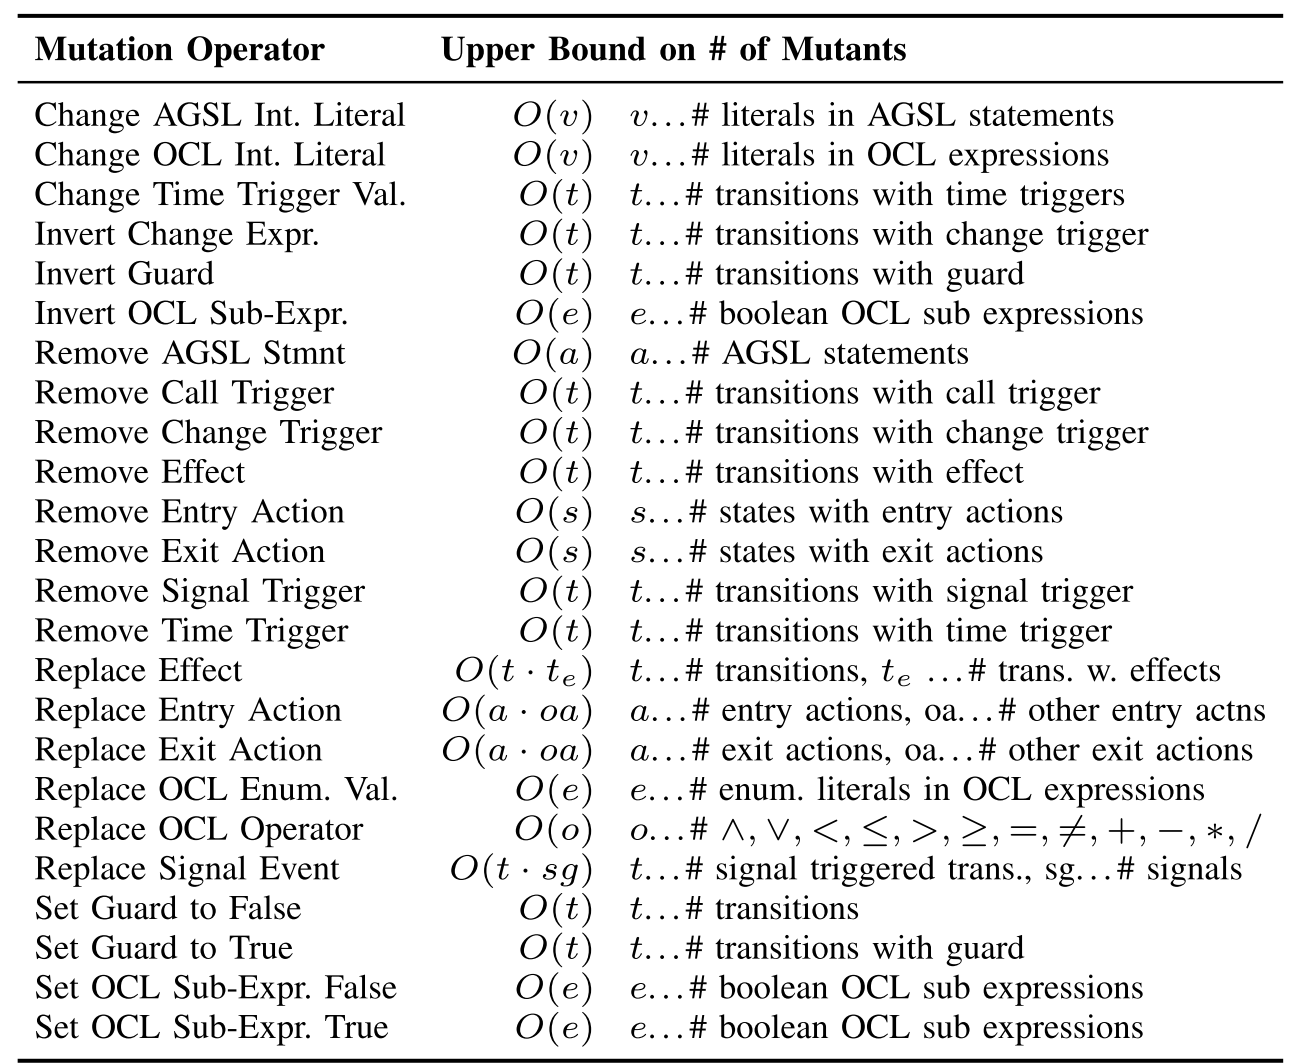
\includegraphics[width=0.6\textwidth]{images/aichernig2015}
%      \caption{Mutation operators introduced in \cite{Aichernig2015}.}
%\end{figure}
%
%%Test cases are generated by choosing a trace within the product graph starting from the initial state and ending at a fail state. Action systems usually describe non-deterministic behaviour, i.e. there can be multiple observable actions enabled at the same time and an implementation is allowed to choose among them. So, whenever there is a branch on observables in the product graph along the chosen trace to the fail state, this branch also is copied into the generated test case, yielding an adaptive test case.
%
%
%
%Model-based data mutation is not only applicable to UML models, in fact, Siavashi et al.~\cite{Siavashi2018} presented a model-based mutation testing approach for evaluating the authentication and authorization of web services in a multi-user context. The modeling of the web service and its security requirements are performed using an UPPAAL timed automata, the model is then mutated to create invalid behavior which is used for test generation to reveal faults in the SUT.
% 
%In model-based mutation testing (MBMT), the original test model is altered systematically by mutation operators creating multiple versions of a model, known as mutant models. The mutants can be used for automatic generation of invalid test inputs that are executed against the SUT. The goal in MBMT is to find whether any invalid tests can pass the testing, thus they can reveal unexpected behavior (i.e., a fault) in the SUT. Hence, MBMT can expose the mistakes that are caused by missing requirements or incorrect implementation.
%
%In the paper, authors model a web service, its users, and their authentication and authorization requirements. The model is then mutated to create invalid test inputs that target faults in the implementation of the web service. 
%
%Mutation testing extends the fault detection capabilities of MBT by exposing more vulnerabilities of systems. It changes a system's program or its specification, to create new versions of the system. 
%Mutation operators are rules that establish the mutants by altering the syntax of the program (or the specification). The generated tests exhibit altered inputs (including faulty inputs) and input sequences against the SUT. Hence the mutants allow testing of the SUT with invalid inputs. 
%
%The paper introduces eight mutation operators for timed automatas, five operators concern to action elements, and three to guard elements of the automata.
%
%\begin{table}[h!]
\begin{center}
\footnotesize
\begin{tabular}{|p{5cm}|p{10cm}|}
\hline
\textbf{Fault}&\textbf{Description}\\
\hline
Change Name of Actions (CN) & Replaces the name of an action with the name of other actions in the model. Thus, the expected sequence of the inputs to the implementation will be different..\\
Change Target of Actions (CT) & Changes the target location of an action to another location in the model. This operator breaks the flow of test inputs and violates the state of the model. Both input and output actions can be mutated by this operator.\\
Change Source of Actions (CS)& Changes the source location of an action to another location. Similar to CT, this operator mutates the sequence of input/outputs. \\
Remove Actions (RA)& randomly deletes one action at a time and creates a mutant. Omitting an action will manipulate the sequence of input/output actions.\\
Duplicate Actions (DA)& randomly copies an action in different parts of a model, thus alternates the sequence of inputs and outputs by repeating actions in unexpected states of the model.\\
Remove Guards (RG)& randomly selects an action and removes its guard. Actions that are mutated by RG will be always enabled.\\
Change Guards Logical Operators (CGL)& changes logical operators (i.e., ==, <=, >=, !=, < and >) in guards.\\
Change Guards Variables (CGV) & alters values of the variables that are used in guards and creates additional mutants that cannot be defined by other mutation operators\\
\hline
\end{tabular}
\end{center}
\caption{Fault Model from \cite{Siavashi2018}}
\label{table:faultModel:Siavashi}
\end{table}%

%
%%\textbf{MutRex: A Mutation-Based Generator of Fault Detecting Strings for Regular Expressions}
%
%Similarly, Arcaini et al.~\cite{Arcaini2017} proposed a model-fault-based approach for generating tests for regexes. The work is based on an automata representation of regexes that generates distinguishing strings exposing the faults introduced in mutated versions of a regex under test. The paper also introduces fault classes representing possible mistakes a user can make when writing a regex.
%
%The proposed tool, MutRex, first produces some mutants from a regex $r$ according to some fault classes representing common mistakes that are made when writing regexes; then, for each mutant $m$, it generates a string $s$ able to distinguish $m$ from $r$, i.e., a string that is evaluated differently in $r$ and $m$ (in terms of mutation testing, $s$ kills $m$). The set of generated strings is a test suite able to detect all the seeded faults.
%
%The authors identified three families of faults: \textit{single character faults}, \textit{character class faults} are respectively related to wrong uses of single characters and character classes, instead \textit{other faults} are related to wrong uses of the multiplicity and of the negation operator.
%
%\begin{table}[h]
%\caption{Mutation operators implemented by MutRex}
%\label{table:MutRex}
%\tiny
%\begin{tabular}{|p{3cm}|p{11cm}|}
%\hline
%\multicolumn{2}{|c|}{Single character faults}\\
%\hline
%Case Change CC & Regexes are case sensitive. However, a user could use them without being aware of this, or she could simply use the wrong case (either upper or lower). This operator mutates a regex r by changing the case of characters appearing in r: a mutant is created for each character of r not used in a character class, and a mutant is created for each character.\\
%Case Addition CA&This operator is similar to CC, but makes both lower and upper cases possible when only one of the two is used: for each character of the regex r not used in a character class it creates a mutant with the other case of the char added as alternative; for each character class, instead, the mutant adds as alternative a new character class having the extremes of the interval in the other case.\\
%Metachar to Char M2C& In a regex, some characters can be interpreted as metachars or chars depending on the context, and there is no mandatory special way to identify metachars. For example, character '-' is interpreted as a metachar only in character classes, otherwise it matches the normal dash character. A user may want to use a char c, but she could wrongly use c as metachar. This operator transforms a regex r containing a char c interpreted as a metachar in a regex r' in which c is interpreted as a char. Note that the way to mutate r depends on the metachar c: for example, M2C applied to '-' removes the character class where '-' is used.\\
%Char To Metachar C2M & In other cases, instead, the designer wants to use a metachar c, but, because of the context, c is interpreted as a simple char. This operator transforms a regex r containing a c interpreted as a char in a regex r' in which c is interpreted as a metachar. Similarly to M2C, the way to mutate r depends on the metachar c.\\
%\hline
%\multicolumn{2}{|c|}{Character class faults}\\
%\hline
%Character Class Creation CCC& Character classes are delimited by square brackets []. A user may want to use a character class and forgets (or ignores) the parentheses. Given a regex $r = c_{1}-c_{2}$, the operator mutates $r$ in $r'= [c_{1} - c_{2}] $.\\
%Character Class Addition CCA&The user could have forgotten a given interval in a set of character classes. Given a regex $r = [cc_1 ... cc_n]$, the operator creates a mutant $r' = [cc_1 ... cc_n cc_{new} ]$ for each $cc_new$ not present in r; $cc_{new}$ can be a-z, A-Z,or 0-9.\\
%Range Modification RM&The user could have specified the operator produces a mutant in which $c_1$ or $c_2$ is increased a too tight or too broad interval. Given a regex $r = [c_1 - c_2]$, or decreased (if it is still a valid char). \\
%Character Class Restriction CCR& The user could have written a regex that is too permissive since it accepts characters that should not. Given a regex $r =[cc_1 ... cc_n]$, the operator creates a mutant $r' = [cc_1 ... cc_{i-1}cc{i+1} ... cc_n]$ for each $cc_i$ (i.e., it removes an interval from the character class).\\
%Prefix Addition PA& Sometimes all the characters of a string $s$ satisfy some constraints, except for the first character in $s$ that must satisfy additional constraints; for example, identifiers in most programming languages cannot start with a number. This mutation operator, given a repeat expression regex $r =[cc_1, ..., cc_n]m$ (being $m$ the multiplicity), introduces a prefix that is one of the different character classes $cc_1, ..., cc_n$ used in $r$. The obtained mutants are as follows: $[cc_1][cc_1, ..., cc_n]m, [cc_2][cc_1, ..., cc_n]m, ..., [cc_n][cc_1, ..., cc_n]m$.\\
%Character Class Negation CCN& Regex [ˆ$cc_1 ... cc_n]$ matches any character that is not listed in the character classes $cc_1, ..., cc_n$. The designer could have forgotten the ˆ symbol and written $[cc_1 ... cc_n]$. CCN introduces symbol ˆ it creates a mutant in which all the character classes are excluded (i.e, [ˆ$cc_1 ... cc_n$]), and a mutant for each character class $cc_i$ in which only $cc_i$ is excluded (i.e, $[cc1] | ...| [$ˆ$cc_i] | ...| [cc_n])$.\\
%
%Negated Character Class to Optional NCCO& Another common error regarding the use of a negated character class [ˆcc] is that it requires 'to match a character that is not listed' and not 'to not match what is listed'. Therefore, a negated character class still requires to match a character. A user could misunderstand the semantics of the operator, thinking that it simply excludes the character; in some cases, for example at the end a word, she could be interested in accepting also no character. Operator NCCO makes ˆ optional, i.e., it mutates [ˆcc]in[ˆcc]?\\
%\hline
%\multicolumn{2}{|c|}{
%Other faults}\\
%\hline
%Negation Addition NA&In a regex $r = r_1r_2 ...r_n$, the user could forget a negation ˆ. The operator creates a mutant adding a negation wherever possible in $r$, i.e., ˆ$r_1r_2 ...rn, r_1$ˆ$r_2r_n, ..., r1r2 ... $ˆ$r_n$. \\
%Quantifier Change QC&The user could have used the wrong cardinality. The operator mutates each simple repeat quantifier in another simple quantifier; moreover, for each user-defined quantifier, it creates a mutant in which $n$ (or $m$) is increased and a mutant in which it is decreased.
%Example\\
%\hline
%\end{tabular}
%\end{table}
%
%
%A mutant $m$ of a regex $r$ can modify the accepted language in four ways: 
%\begin{itemize}
%  \item Arbitrary edit: some words are added to the language and other words are removed.
%  \item Generalization: some words are added to the language and no word is removed.
%  \item Specialization: some words are removed from the language and no word is added.
%  \item Equivalent: the mutant is equivalent and so the two languages are the same.
%\end{itemize}
%
%
%%\textbf{Combinatorial mutation approach to web service vulnerability testing based on SOAP message mutations}
%
%In a different context, Li et al.~\cite{Li2012} proposed a model-based combinatorial mutation approach based on SOAP messages for Web service vulnerability testing.
%The technique presented in the paper consists of (1) analyzing the web service methods and identify all the associated web service methods. (2) Invoke different sets of mutation operators according to the perturbation policy on the SOAP messages (XML documents) by parsing the WSDL files, and then (3) call the appropriate combinatorial testing approach to generate combinatorial test cases.
%
%The XML model-based approach presents the following two perturbation policies: data value and interaction perturbations. Both perturbation policies directly act on the SOAP messages. The former one modifies values in SOAP messages according to their data types while the latter one may consider the data values and data relationships. Part of the mutation operators bear double effects of data value and interaction perturbations.
%
%The following mutation operators were introduced:
%
%\begin{figure}[h]
%  \centering
%    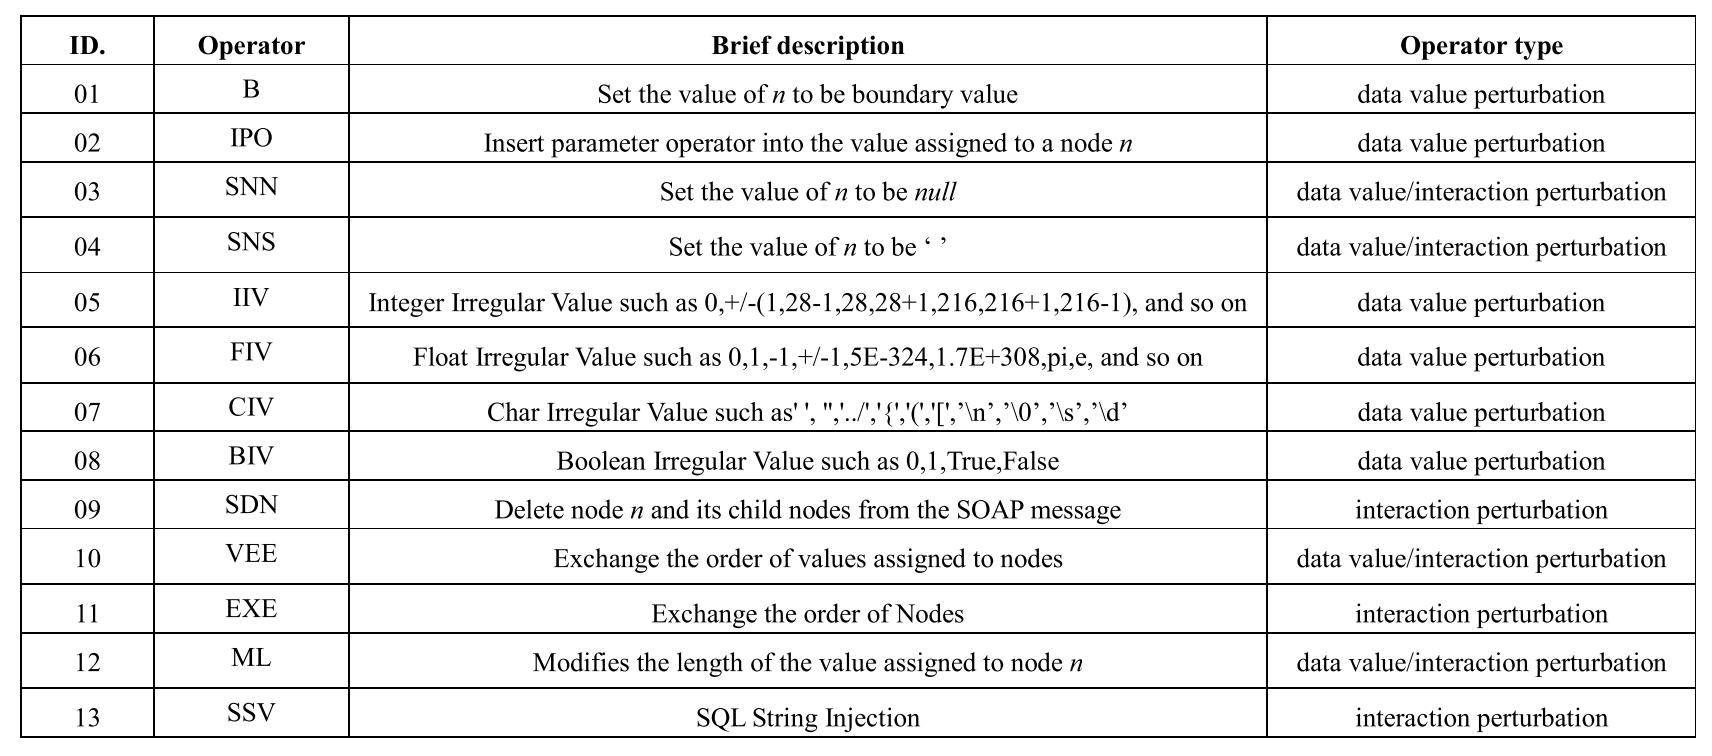
\includegraphics[width=\textwidth]{images/li2012}
%      \caption{Combinatorial mutation approach to web service vulnerability testing based on SOAP message mutations \cite{Li2012}}
%\end{figure}
%
%%\textbf{Worst-input mutation approach to web services vulnerability testing based on SOAP messages}
%
%Similarly, Chen et al.~\cite{Chen2014} introduced a model-based mutation approach for testing web service vulnerability of SOAP messages. 
%
%The method involves partitioning the input domain into sub-domains according to the number and type of SOAP message parameters in the TCFN (test case farthest neighbor) and then selecting the candidate test case whose distance is the farthest from all executed test cases and applying it to test the Web service.
%
%Web service vulnerability refers to flaws in the service that threaten the security of the computer system, for example, memory leaks, buffer overflows, and cross-boundary access (where memory variables access areas outside their defined scope)
%
%SOAP is a message protocol based on an XML document, which forms the basis of the mutation object. The paper introduces 15 mutation operators for SOAP parameters types combined with Web service features.
%
%\begin{figure}[h]
%  \centering
%    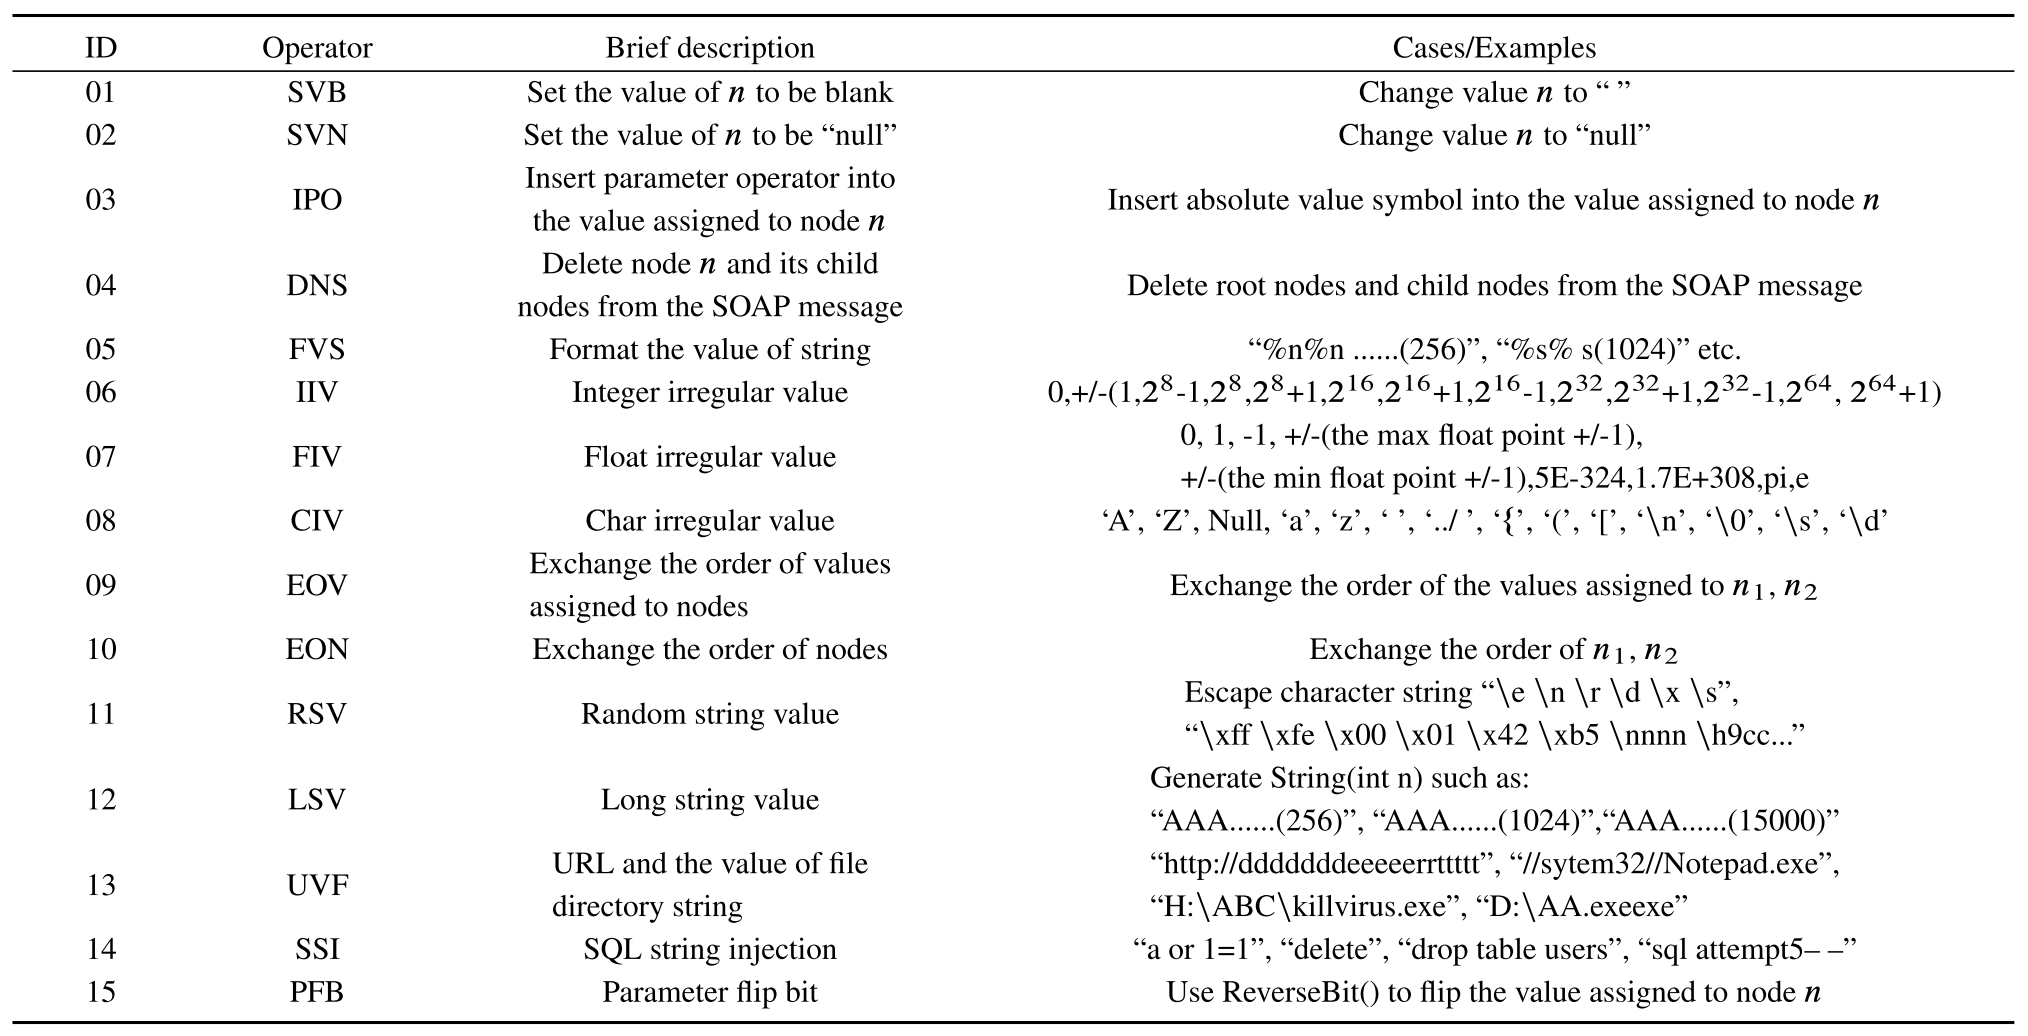
\includegraphics[width=0.8\textwidth]{images/chen2014}
%      \caption{SOAP messages mutation operators.}
%\end{figure}
%
%
%\subsubsection{Search-based data mutation}
%
%Search-based data mutation relies on an evolutionary algorithm to perform model-based data mutation and optimize multiple objectives:  
%cover all the classes of the data-model, cover all the possible faults of the fault model, cover all the clauses of the input/output constraints,
%maximise code coverage~\cite{di2015evolutionary}.
%The coverage of each objective is encoded by means of boolean arrays; this information is used to select a minimal set of inputs that maximize the coverage of the different objectives.
%At every iteration, the evolutionary algorithm keeps only inputs that contribute to increase the coverage of at least one of the objectives (e.g., inputs that cover one instruction not covered by other inputs).
%
%An additional source of information concerning the adoption of fuzzing and grammar-based approaches to perform test input generation is the \emph{Fuzzing Book}~\cite{fuzzingbook2019:GrammarFuzzer}.
%
%
%\subsection{Automated Detection of Equivalent and Redundant Mutants}
%\label{sec:dataequivalent}
%
%Data-driven mutation operators may lead to the generation of both equivalent and redundant mutants.
%In the data-driven context, equivalent mutants consist of modified data (i.e., data altered by means of mutation operators) that do not lead to any noticeable difference in the output of the SUT with respect to the original version of the data.
%Please note that an equivalent mutant differs in content from the original data (i.e., the data chunk has been altered).
%The possible reasons why a mutant may not lead to noticeable differences in the output of the SUT are three. First, changes may go unnoticed because they alter portions of the data that is not read by the SUT. This includes cases in which mutations alter the structure of the input data in such a way that the resulting mutated data is different from the original but still respect the data format. This might happen, for example, when a mutation operator swaps the CDATA section of an XML file and the SUT ignores CDATA content. Second, mutations may alter some of the outputs of the SUT but the test suite oracles ignore that portion of the output. This might happen in a data acquisition system that copies the data payload of network packets in a database; in such a context, a data mutation that alters the message and update the packet checksum might go unnoticed because the SUT would simply copy the message content to the database and the test suite may simply check if the database contains a new message. Third, mutations may alter valid existing data but produce data that is still valid. This often reflect a poor choice of mutation operators; indeed, the selected mutation operators should guarantee to introduce a fault in the data exchanged by the system.
%
%
%Redundant mutants cause the same failures in the test suite. Two are the reasons for redundant mutants. First, the mutations alter different instances of a same data structure in the same way (e.g., delete a message in a sequence). Second, the mutations alter data chunks that are ignored by the oracles of the test suite.
%
%Concrete examples of equivalent and redundant mutants are provided in Figure~\ref{fig:data:quivalent}. In Figure~\ref{fig:data:quivalent}, \emph{Mutation 2} leads to an equivalent mutant since it generates a timestamp that is just one millisecond in the past, which is legal for the system under test. The value 2 for a timestamp, instead, leads to a failure because is considered too much in the past (see \emph{Mutation 1}). To address this problem, engineers should have configured the timestamp field to be mutated by a boundary condition operator (which generates values out of valid range) instead of a bit flipping operator. \emph{Mutation 3}  and \emph{Mutation 4}, instead, are redundant because they both generate a timestamp in the future (under the assumption that \emph{1584889773} captures the current time).
%
%\begin{figure}[h]
%  \centering
%    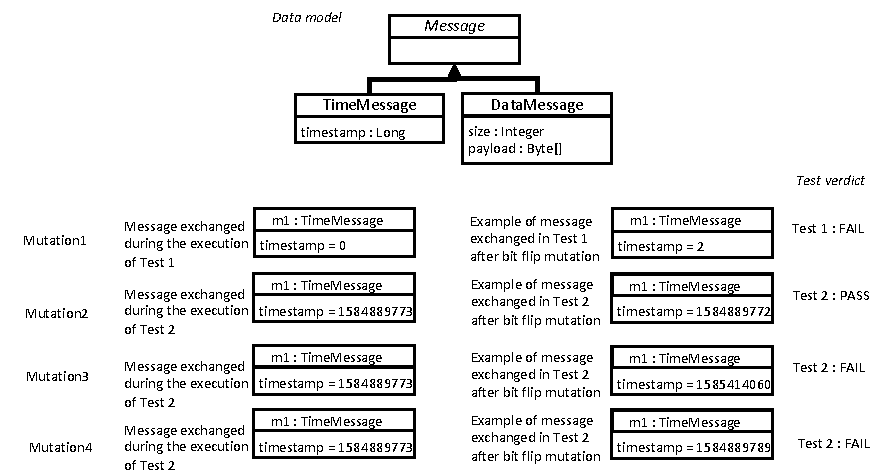
\includegraphics{images/DataDrivenEquivalent}
%      \caption{Examples of data-driven mutations leading to equivalent and redundant mutants.}
%      \label{fig:data:quivalent}
%\end{figure}
%
%Literature lacks approaches to directly target equivalent and redundant mutants. However, some of the solutions implemented in existing data mutation approaches might limit the presence of equivalent and redundant mutants. We observe three main solutions: (1) driving mutations by means of code-coverage, (2) driving mutations by means of coverage of model structure, and (3) use of model-based oracles.
%
%Code-coverage-driven mutations are the ones implemented by many automated fuzzers such as 
%MoWF~\cite{pham2016model} and AFL~\cite{gutmann2016fuzzing}.
%MoWF aims to generate mutated data that triggers the execution of specific code locations. This is done by combining symbolic execution and meta-heuristic search.
%Since each mutated input triggers a different code location, MoWF, in principle, should always lead to mutated inputs that make the software behave differently than with the original input or with other data mutants. However, it does not ensure that the changes in the internal behaviour of the software are reflected in one of its observable outputs.
%Similarly to MoWF, AFL generates inputs that trigger different code locations. The main difference is that it does not target only specific code locations but it aims to exercise all the branches of the program. 
%Similarly to MoWF, AFL does not guarantee that changes in the internal behaviour of the software are reflected in one of its observable outputs.
%Similarly to AFL, any approach relying on meta-heuristic search that include coverage objectives in the fitness function (e.g.,~\cite{di2015evolutionary}) can limit the presence of equivalent and redundant mutants.
%
%
%The coverage of the model structure enables the generation of mutations targeting different portions of a given data model.
%For example, \emph{pFuzzer} generates valid inputs that cover diverse sets of lexical and syntactical features.
%Other approaches~\cite{di2015generating} generate mutants that target different elements of the data structure.
%By targeting different elements of the data, the generated mutants are unlikely to be redundant or equivalent. However, they do not ensure that such differences are reflected in the SUT observable outputs.
%
%
%Model-based oracles, such as OCL constraints capturing expected outputs (e.g., error messages expected in the presence of a specific change of the data) enable the generation of mutants that are not equivalent and not redundant. For example, by ensuring that each mutant affects a model element referenced in a different OCL constraint and that the constraint is evaluated to true, model-based mutation approaches can guarantee that the data mutations lead to observable changes in the SUT output~\cite{di2015generating}.
%
%
%\newcommand{\ONMO}{\mathit{overall}\ \# \mathit{of}\ \mathit{mutation} \ \mathit{operators}}
%\newcommand{\NMOA}{\# \mathit{of}\ \mathit{mutation} \ \mathit{operators} \ \mathit{applied}}
%
%
%\subsection{Analysis of Mutation Testing Results and Mutation Score Calculation}
%\label{sec:data:mutationscore}
%
%In the data-driven mutation testing process, the outcome of the activity \emph{Analyze Results} (see Figure~\ref{fig:data:process}) is a mutation score that is based on
%the percentage of mutants being killed and the percentage of mutation operators applied. 
%The former enables data-driven mutation to achieve objective O1 in Section~\ref{sec:dataProcess}, the latter objective O2. 
%The mutation score can be computed as a weighted average of the percentage of mutants being killed and the percentage of mutation operators applied, according to the following formula
%
%\begin{equation}
%Score=w_{O1} \frac{\# \ \mathit{of}\ \mathit{killed} \ \mathit{mutants}}{\mathit{overall} \# \mathit{of}\ \mathit{mutants}} + w_{O2} \frac{\# \mathit{of}\ \mathit{mutation} \ \mathit{operators} \ \mathit{applied}}{\mathit{overall} \# \mathit{of}\ \mathit{mutation} \ \mathit{operators}}
%\label{f:mutation:score}
%\end{equation}
%
%Where $w_{O1}$ and $w_{O2}$ capture the importance of the objectives O1 and O2, respectively. We assume $w_{O1}$ + $w_{O2} = 1$. In case objective $w_{O1}$ and $w_{O2}$ have the same importance, they should be set to $0.5$. In the case of safety-critical systems, the mutation score should be equal to 1.
%
%In formula \ref{f:mutation:score}, the $\mathit{overall}\ \# \mathit{of}\ \mathit{mutants}$ corresponds to the number of test executions in which at least one data object have been altered through mutation. We refer to such test executions as \emph{mutated test executions}.
%The $\# \ \mathit{of}\ \mathit{killed} \ \mathit{mutants}$ corresponds to the number of \emph{mutated test executions} that either failed or during which a redundancy mechanisms has been activated to handle the mutated data.
%
%The $\ONMO$ corresponds with the number of different mutations that can be applied to the data, according to the data model. It depends on the strategy adopted to select the items to be mutated.
%% and may vary based on the strategy adopted to perform data mutation.
%For approaches relying on \textbf{UML models}, one possibility is to follow the approach of Di Nardo et al.~\cite{di2015generating}, which consists of mutating every model element (e.g., class or class attribute in the class diagram capturing the data model) with every mutation operator that is applicable to the specific model element, according to the fault model captured in the class diagram (see Section~\ref{sec:data_operators}).
%The $\ONMO$ (ONMO) could be thus computed as the sum of the number of applicable mutation operators for ever every model element.
%The $\NMOA$, (NMOA) consequently, should capture the number of mutations that were performed. In the approach of Di Nardo et al.~\cite{di2015generating}, NMOA corresponds to the number of model elements for which at least one instance had been mutated. 
%
%For the computation of ONMO and NMOA, a strategy similar to the one presented by Di Nardo et al. can be used also in the case of approaches relying on \textbf{grammars} or \textbf{block models}. Indeed, also for these two types of approaches, data mutation is performed by means of a set of mutation operators that are applied in the presence of specific data types. 
%These data types correspond to the production rules of the grammar or the blocks defined in the block model. 
%Approaches that do \textbf{not require an input model} typically work at the bit/byte level. In these cases, ONMO might be calculated as the number of available operators, or
%as the number of bit/bytes in the inputs multiplied by the number of applicable mutation operators.
%
%
%Moreover, data njection has been usually used to asses the robustenss of software here we apply to assess the test suite with respct to interoperability faults.
%%this is the first work relying on data fault injection procedures to perform mutation analysis.

% !TEX root = MAIN.tex

\clearpage
\section{Code-driven Mutation Testing}
\label{sec:back:testGeneration}

This section describes the approaches that can be adopted to automatically generate test cases that kill mutants.
To kill a mutant we need test cases that (1) reach the mutation point (i.e., execute the mutated code), (2) cause 
corruptions
in the program state right after the mutated code,
and (3) manifest these corruptions into the program output 
(e.g., by producing an erroneous value in a state variable verified by a test assertion) 
thus leading to a failure~\cite{papadakis2019mutation}. These conditions are also known as the \INDEX{killing conditions} of a mutant.

In the literature, there exist two groups of approaches for 
generating test cases that kill mutants:
approaches based on constraint-programming, and approaches based on evolutionary computation. Below we introduces these two stream of approaches after introducing two well-known solutions for test generation driven by structural coverage, which are the basis for mutation testing solutions based on constraint programming.

\subsection{Test Generation driven by program structure}
\label{sec:back:generation:structure}
Two alternative state-of-the-art solutions to generate test inputs that maximize structural coverage are CBMC, a bounded model checker, and KLEE~\cite{cadar2008klee}, a symbolic execution engine. They are detailed below.

%\subsubsection{CBMC}
%\label{subsec:cbmc}

\INDEX{CBMC} is an approach that implements \INDEX{Bounded Model Checking}~\cite{BiereCCZ:TACAS99,SeryFS:ATVA12} (BMC), an approach for purely static software verification.
The idea in BMC is to represent the software together with the
properties to be verified as an instance of the propositional
satisfiability problem (SAT).  Such a representation captures the
software behavior exactly, assuming that all the loop bodies in the
software are repeated at most a fixed number of times.
This approach has several advantages: the logical formulation is usually
very compact compared to traditional model checking, where verification
is reduced to a reachability problem in a graph representing the program
state space;
%
there are several high-performance SAT
solvers~\cite{MarquesSilva:IEEETRAN99,EenS:SAT2003} that can be used for
solving the instances;
%
and the satisfying assignments of an instance can be directly translated
to meaningful counterexamples for correctness in the form of
fault-inducing executions.
%
Furthermore, it is widely recognized that BMC based approaches are particularly good
at quickly finding short counterexamples when they exist.

%A {\em bounded model checker} takes as input a program $\prog$, a bound $k$
%for loop unrolling, and a set $S$ of properties to be verified against
%$\prog$, and returns for each property ${l}$ in $S$, expressed as a propositional statement over variables of $\prog$ at a location $l$, either \vspace{-0.2cm}
%\begin{itemize}
%    \item \emph{verified}, if the executions of $\prog$  satisfy $\prop{l}$;\vspace{-0.25cm}
%    \item \emph{unreachable}, if no execution of $\prog$ reaches $l$;\vspace{-0.25cm}
%    \item \emph{false}, if there is an execution of $\prog$
%    where the property $l$ is broken; and\vspace{-0.25cm}
%    \item \emph{unknown}, if the checker is unable, due to
%    memory or time limits, to determine whether ${l}$ holds,\vspace{-0.2cm}
%\end{itemize}
%under the assumption that no loop body in the program is repeated more
%than $k$ times.
%
%The approach is naturally a compromise between practicality and
%completeness.
%As the SAT problem is \INDEX{NP-complete}, determining whether $\prop{l}$ holds
%requires in the worst case exponential time with respect to the size of
%the SAT instance for all known algorithms.
%%
%Furthermore, the instances can in some cases grow very large since many
%operations, such as multiplication, have quadratic encodings in SAT and,
%for example, the instance grows exponentially in number of nested loops.
%%
%
%Due to numerous optimizations BMC can nevertheless solve many practical
%problems in reasonable time and memory limits.
%%
%For example, the size of the resulting SAT instance can be dramatically
%reduced by slicing off parts of the program that do not affect the
%validity of the property being checked, and
%%
%extremely efficient SAT solver implementations which learn the instance
%structure and use adaptive heuristics~\cite{MahajanFM:SAT04} rarely
%suffer from the exponential worst-case behavior in problems emerging
%from applications.
%%
%The fact that bounded model checkers only prove correctness of
%properties for executions not exceeding the bound $k$ is also beneficial
%in many ways for detecting regressions.  In addition to obvious
%performance benefits our experiments show that in most cases even a single
%loop iteration is sufficient to indicate a regression between two
%versions, and a small bound guarantees in a natural way that the
%reported counterexamples are short.

%\subsubsection{KLEE}

\INDEX{KLEE}~\cite{cadar2008klee} is an open source tool that implements {\INDEX{Concolic Execution}}, a technique that performs \INDEX{symbolic execution} along a concrete execution path. KLEE was designed to automatically generate test cases that achieve high code coverage. The tool is implemented as a modified LLVM virtual machine that targets LLVM bytecode programs.
KLEE also provides a symbolic POSIX library that enable analysis of programs that uses the system's environment. For example, KLEE can be executed with the flag \texttt{-sym-stdin N} which will make stdin symbolic with size \texttt{N}.  

In FAQAS, we rely on KLEE to automatically produce the inputs that make the mutated version of the program generate a different output than the original version.



\subsection{Test Generation based on Constraint Programming}
\label{sec:testGen:CP}

Techniques based on constraint programming use some form of automated reasoning (e.g., Propositional Satisfiability or Constraint Solving~\cite{SATandCPsurvey:2006}) to derive data that satisfy all the conditions necessary to kill a mutant~\cite{offutt1997automatically}.Existing approaches, differ for the strategy adopted to automatically generate these constraints from the program under test.

Offutt et al.~\cite{offutt1997automatically}, for example, automatically derive such constraints from the program by extracting the predicate expressions on the program's control flow graph.
Then, such constraints are encoded to form a constraint system. In their approach, they propose three strategies for identifying infeasible constraint systems, the contradictions to such systems are the new test cases for the program under analysis.

% !TEX root =  ../MutationTestingSurvey.tex

\begin{lstlisting}[style=CStyle, caption=midval function returns the mid value between three integers., label=midval, mathescape=true]
int midval (int x, int y, int z) {
	int midval;

	midval = z;
	if (y < z) {
		if (x < y) {
			midval = y;
		}
		else if (x < z) 
 $\Delta$ else if (x <= z) {
			midval = x;	
		}
	}
	else 
		if (x > y) {
			midval = y;
		} else if (x > z) {
			midval = x;
		}
	return midval;
}
\end{lstlisting}

In the following, we introduce an example of the application of Offutt's~\cite{offutt1997automatically} approach by using the \texttt{midval} function presented in Listing~\ref{midval}. This function has a mutation on line 9, which has been mutated into line 10. According to their approach, the three killing conditions would be the following:

\begin{itemize}
	\item Reachability $C_R: (y < z) \wedge (x \geq y)$
	\item Necessity $C_N: (x < z) \neq (x \leq z)$
	\item Sufficiency $C_S:$ Output(P) $\neq$ Output(M)
\end{itemize}

$C_R$ defines the condition required to reach the mutated statement, in this case the conjunction between the predicate of the first if condition and the negation of the second if condition. $C_N$ defines the condition required to assure a different program state between the original and mutated version of the program right after the mutation point. Finally, $C_S$ defines the condition necessary to demonstrate that both the original and the mutated program returns different values.

Holling et al.~\cite{holling2016nequivack} proposed to use a \INDEX{symbolic execution} approach to identify new test cases. Their idea is to first execute symbolically both the original and the mutated function, then to check if their return values are equivalent or not. 
Symbolic execution determines what inputs cause each part of a function to be covered during execution. To symbolically execute a function, it is necessary to replace the original inputs (i.e., concrete values) with symbolic ones. The \INDEX{symbolic values} represent a set of possible concrete values that lead to a certain program path (i.e., path condition). 


Holling's approach~\cite{holling2016nequivack} to automatically identify equivalent mutants relies on the observation that 
two mutants are equivalent when there are no concrete values making the mutated function produce an output that is different from the one of the original function.
If a value that makes the two functions generate distinct results can be found, the mutant is non-equivalent.
To automate the generation of inputs, Holling et al. rely on KLEE~\cite{cadar2008klee}.

We introduce an example of Holling's approach in Listing~\ref{function}. The top part of Listing~\ref{function} shows the function \texttt{isPositive}, which checks if an integer number is positive or not. The bottom part of Listing~\ref{function} presents the mutated version of \texttt{isPositive}, where the relational operator $\geq$ has been replaced by the operator $>$.
To automate the generation of inputs using KLEE, all the parameters need to be treated as symbolic values.
%F: "the \texttt{isPositive} parameter \texttt{num}" it's impossible to understand what is the parameter and who owns the parameter
%In Holling's approach, first, the \texttt{isPositive} parameter \texttt{num} needs to be treated as symbolic value, which is done by the function \texttt{make\_symbolic} (see Listing~\ref{example}) which converts concrete variables to symbolic by considering its memory address and size. 
This is achieved by function \texttt{make\_symbolic} (see Listing~\ref{example}) which converts concrete variables to symbolic ones by considering their memory address and size. 
%F: please fix
In Listing~\ref{example}, the parameter \texttt{numSymbolic} is made symbolic in Line 3. Then, the original and mutated functions are called using the symbolic arguments in Lines 5 and 6.
%Finally, the \texttt{assert} function of line 8 verifies if the integer return values of both functions are equal or not.
Finally, we need to introduce an assertion that makes the symbolic execution engine \EMPH{look for inputs that make the output of the two functions different}. 
In Listing~\ref{example}, this is achieved with an assertion that verifies that the return values of the two functions the same (see Line 8). 
Despite being counter-intuitive, this approach is effective because symbolic execution engines aim to identify inputs that falsify the assertions in the program. 
When the equality is falsified, then the two functions can produce a different output for a same input.
The input that falsifies the equality can thus be used to improve the test suite enabling it to kill the mutant.
In the example of Listing~\ref{example}, KLEE will indicate that the return values of the original and mutated function differ when \texttt{num} is equal to zero.
A new test case exercising function \texttt{isPositive} with \texttt{num=0} should thus be added to the test suite in order to kill the mutant.

\begin{lstlisting}[style=CStyle, caption=isPositive and MUT\_isPositive functions, label=function]
int isPositive(int num){
	if (num >= 0){
		return 1;
	} else {
		return 0;
	}
}

int MUT_isPositive(int num){
	if (num > 0){
		return 1;
	} else {
		return 0;
	}
}

\end{lstlisting}

\begin{lstlisting}[style=CStyle, caption=Holling's approach for test case generation., label=example]
void test () { 
	int numSymbolic; 
	make_symbolic(&numSymbolic, sizeof(numSymbolic), "numSymbolic"); 
 	
 	int original_ret = isPositive(numSymbolic); 
	int transformed_ret = MUT_isPositive(numSymbolic); 
 
	assert(original_ret == transformed_ret); 
}
\end{lstlisting}

Similarly to Holling's approach, Riener et al.~\cite{riener2011test} proposed to use \INDEX{bounded model checking} techniques to search for these counter examples.
In their bounded model checking approach, the original program and the mutant are unrolled with respect to a certain maximum bound. In program unrolling, loops are re-written as a repeated sequence of similar independent statements. Then, both unrolled programs are encoded into a logic formula over the same input variables. To ensure that the mutation affects the output of the mutant, a propagation condition is encoded and added to the previous logic formula, the condition asserts that there exist at least one pair of different outputs under the assumption of equal inputs. In the last step, the formula is processed by a SMT-solver, if the solver finds a satisfying assignment, the inputs of the formula are translated into a new test case for the current program under analysis.

%Compared to symbolic execution, one advantage of bounded model checking is that it does not require to execute the whole program but may focus on the mutated functions only.

%To reduce the time required by the symbolic execution process, which needs to be performed against all the mutants of the software, Papadakis et al.~\cite{papadakis2011automatically, papadakis2010towards} propose to combine symbolic execution techniques and \INDEX{mutant schemata} to automatically generate test cases targeting the killing conditions induced by the different mutants embedded into the same executable. The approach targets \INDEX{weak mutation} testing and may not generalize to strong mutation testing. Indeed, ensuring the sufficiency property (i.e., verify that changes are propagated to outputs) for multiple mutants might lead to scalability issues not addressed by the proposed approach.





\INDEX{SEMu}~\cite{chekam2021killing} is a recent mutantion testing  framework based on dynamic symbolic execution that has been built on top of the KLEE Symbolic Virtual Machine~\cite{cadar2008klee}.
SEMu uses a form of \INDEX{differential symbolic execution}~\cite{person2008differential} to generate test inputs that kill mutants. The approach consists of modeling the mutant killing problem as a symbolic execution search in a scalable and cost-effective way. 
The SEMu framework is the building block of 
%act as a baseline for 
the test generation tool developed in FAQAS (i.e., \INDEX{SEMuS}). Different from the approaches presented above, SEMu can generate test inputs that kill mutants without the need of human intervention (e.g., to ad assertions); however, it targets only bash programs, it cannot generate unit test cases, for example.

%To kill a mutant, we need test cases that capture the three killing conditions of a mutant~\cite{offutt1997automatically}: 
%\begin{itemize}
%	\item \INDEX{reachability}: the test case should execute the mutated statement
%	\item \INDEX{necessity}: the test case should cause an incorrect intermediate state, if it reaches the mutated statement
%	\item \INDEX{sufficiency}: the final state of the mutated program should differ from the one of the original program
%\end{itemize}

%\DONE{the concept of "mutation point is not clear"; you do not clarify that the two versions are compiled in the same executable}

In SEMu, the multiple program versions (i.e., the original and the mutated programs) are compiled within the same executable. 
Because mutants differ only slightly from the original program (minor syntactic differences), the technique performs one symbolic execution search for the unchanged source code, and then it forks the symbolic execution search every time it reaches a mutated statement.

The technique follows both the mutated and the original execution and compares the state (i.e., the value of the variables) at each step of the execution.
More precisely,  every time the execution reaches the statement after the mutation, the technique triggers the generation of test inputs for the forked and the original programs by comparing their symbolic states. To generate test inputs that kill the mutant, the technique encodes the three killings conditions, obtained from the symbolic execution search, into a single formula (the $kill$ formula) to be passed to a constraint solver.

%\begin{figure}[tb]
%\begin{center}
%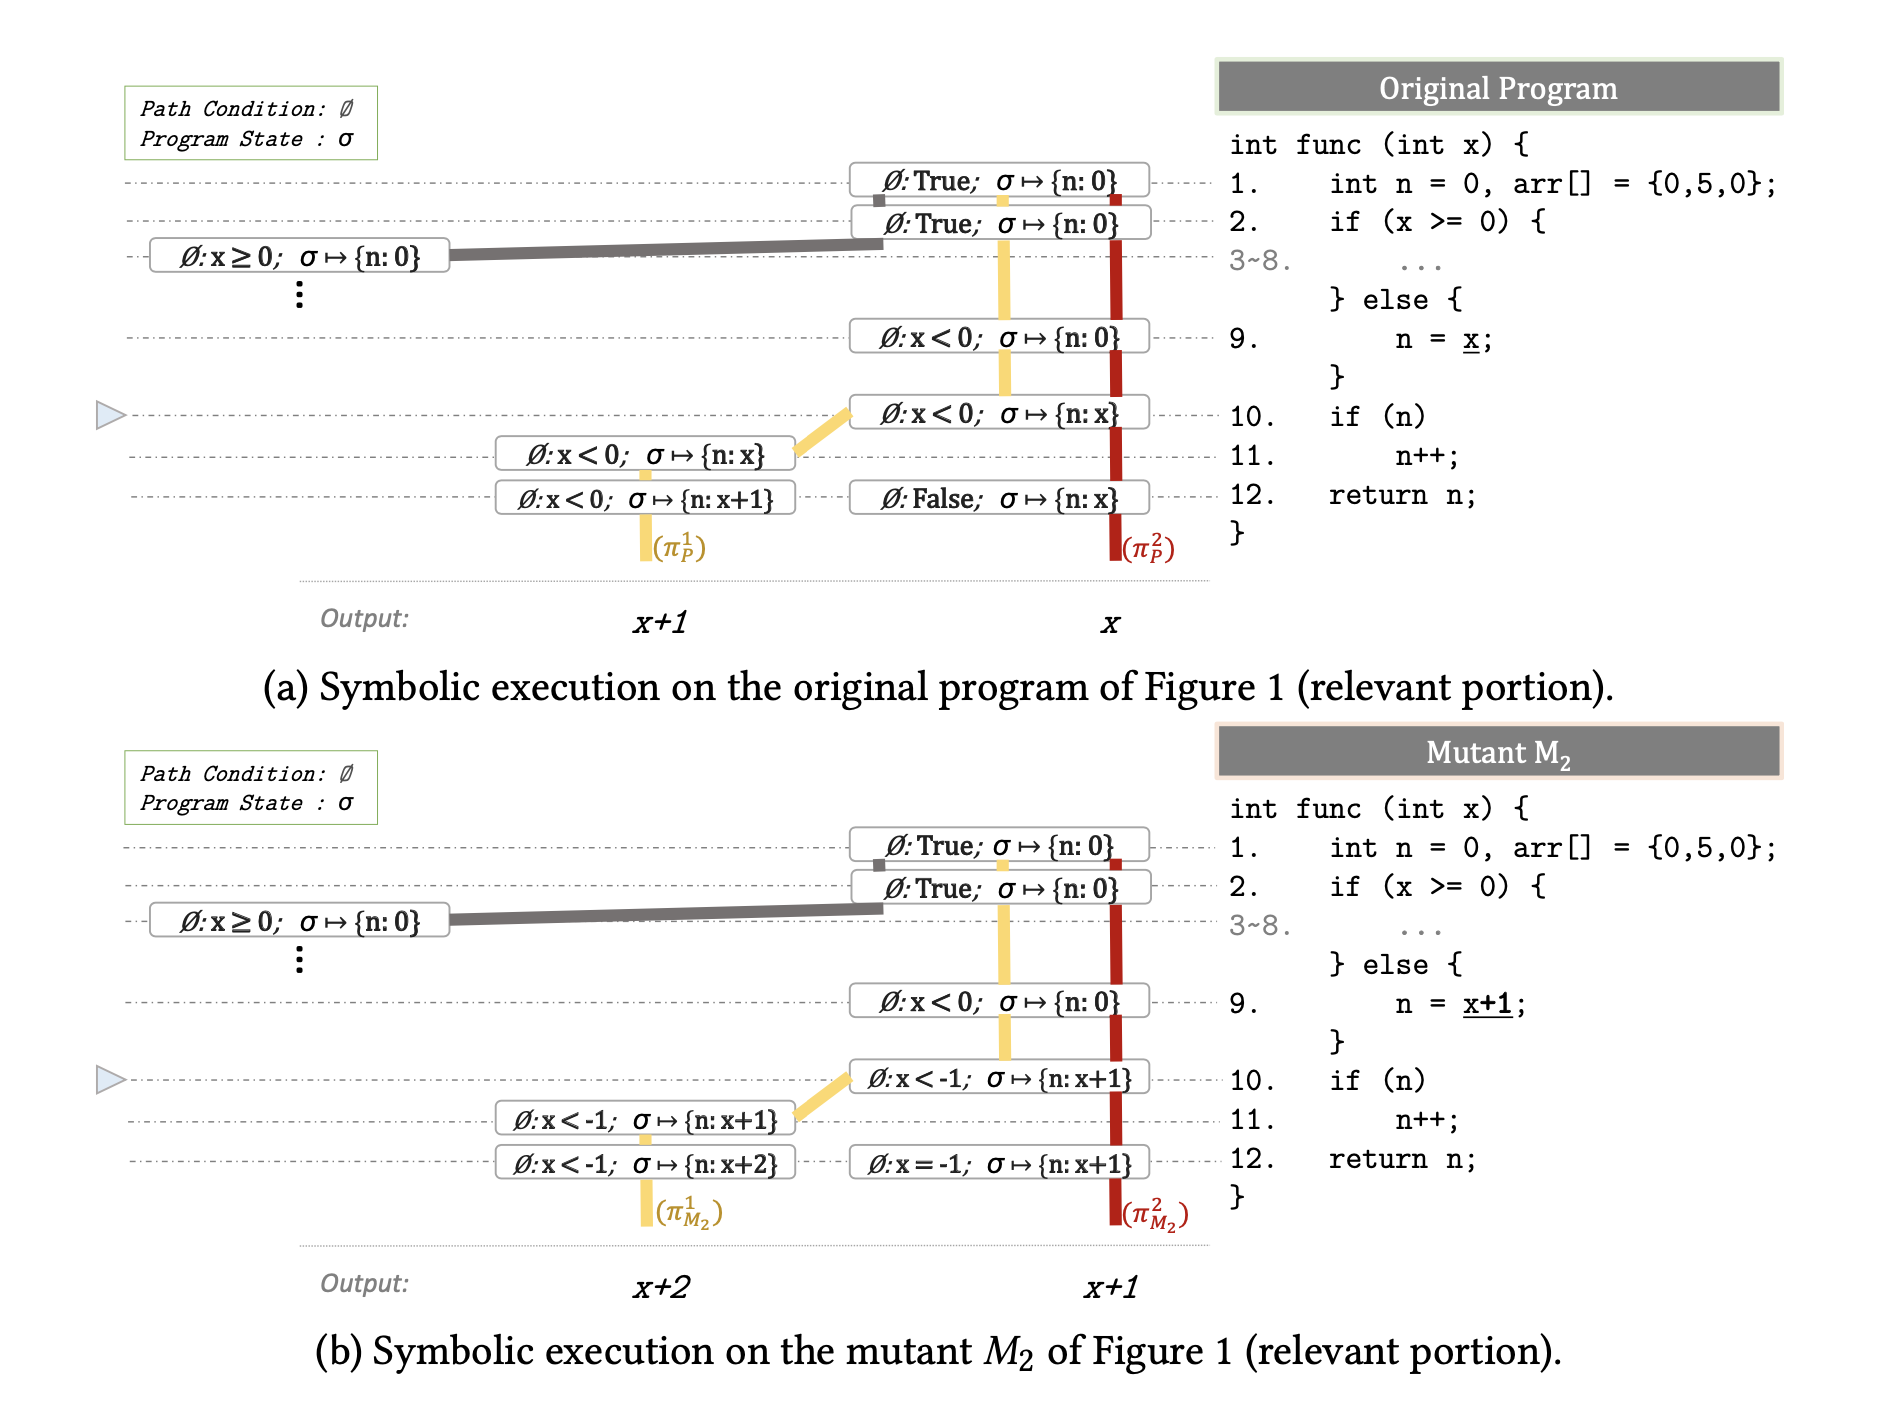
\includegraphics[width=\textwidth]{images/semu-example}
%\caption{SEMu example. Source: Chekam et al.~\cite{chekam2021killing}.}
%\label{fig:semu-example}
%\end{center}
%\end{figure}
%
%Figure~\ref{fig:semu-example} introduces an example of \INDEX{dynamic symbolic execution}, sub-figure (a) shows the symbolic execution for the original program, while (b) shows the symbolic execution process for the mutant version. In order to generate test inputs that kill a mutant, the technique applies symbolic execution to a program $P$ and to its respective mutant $M_2$, to produce their respective symbolic paths. In a second step, the technique solves the formula $kill(\pi_P, \pi_{M_2})$ to generate the test inputs that kills $M_2$ and goes through $\pi_P$ in $P$ and through $\pi_{M_2}$ in $M_2$. 
%As shown in Figure~\ref{fig:semu-example}, symbolic execution on the original program leads to the paths $x < 0$ and $False$, with the respective outputs $x + 1$ and $x$.
%Instead, the symbolic execution on the mutant leads to paths $x < -1$ and $x = -1$, with outputs $x + 2$ and $x + 1$.
%
%Consequently, the only feasible path that targets mutant $M_2$ is the following:
%
%\begin{equation}
%	kill(\pi_{P}^{1}, \pi_{M_2}^{1}) = ((x < 0) \wedge (x + 1 \neq x + 2) )
%\end{equation}
%
%Where the solution to $kill(\pi_{P}^{1}, \pi_{M_2}^{1})$ is $x = -2$.



To speed-up test generation, SEMu integrates a number of optimizations:
\begin{itemize}
	\item \INDEX{Meta-mutation}: all mutants are encoded into a single program called meta-mutant (in FAQAS, we extended it at source code level), the mutant is selected through a branching statement named mutant choice statement.
	\item \textbf{Discarding non-infected mutant paths}: mutant paths failing to infect the program state are discarded immediately.
	\item \textbf{Heuristic search}: stop exploration of a path after $K$ transitions, and solve the kill formula.
	\item \textbf{Infection-only strategy}: Generates test inputs by aiming only at mutant infection.
\end{itemize}

%\DONE{I have the impression that none of the following heuristics are currently used in FAQAS. I would write that we indicate which heuristics are not feasible and which one may be investigated in follow-up activities.}

%To reduce execution time further, SEMu also introduces a list of parametric heuristics that can be controlled by the user; this set of heuristics help to define which paths to explore and in general, the test generation process:

%%\DONE{please use "test cases" not "tests"}
%
%\begin{itemize}
%	\item \textbf{Controlling for reachability} (seeded symbolic execution): This heuristic consists of executing the original program up to a given path using the same inputs provided by existing test cases; the use of concrete inputs helps symbolic execution to quickly prune paths that are infeasible or does not reach the mutant. This feature is inherited from KLEE.
%	%a explore paths in seeded  mode up to a given length. 
%	
%%	\DONE{You are not explained what t does. "This heuristic consists of executing the original program up to a given path using the same inputs provided by existing test cases; it generates symbolic inputs only for...  For its implementation SEMu relies on a feature provided by KLEE"}
%	% This heuristic quickly prunes paths that are infeasible or does not reach the mutant. 
%	
%%	\DONE{Please refine what I wrote in the following. You were not explicitly clrifying hat the problem is.}
%	
%	We do not integrate this feature in the FAQAS framework because of two reasons. 
%	First, SEMu can deal only with test cases for batch programs (i.e., providing arguments to the main function of the software under test), which is different from our context where we either have unit or integration test cases implemented in a specific programming language, or we have complex system test cases simulating communication from ground to orbit through network and a simulator. 
%	Second, in our context, because of the complexity of the SUT we can generate unit test cases but not integration or system level ones. The main difference between such test cases is the entry point, for unit test cases it is the function under test, for integration or system test cases it is a function different than the function under test. Consequently, implementing such solution would require the implementation of additional technology to map the seeds collected for test inputs with different entry points, which is not provided by KLEE.
%
%	\item \textbf{Controlling for propagation}: This heuristic consists of controlling where and how often to verify whether the execution path has propagated the infection (i.e., an erroneous state with respect to the original program) after the execution of the mutated statement; if the mutation does not propagate the infection, the sufficiency killing condition will not be met, and thus it makes sense to prune these paths to decrease the symbolic search space.
%	% sometimes an infected program state fails to propagate the infection to the outputs, these states should be quickly discarded. 
%
%%	\DONE{Rewrite the sentence, unclear}
%	
%	For controlling the propagation of the infected state, SEMu introduces the following four parameters:
%	\begin{itemize}
%%		\item \DONE{(Comments are put above the problematic item) Unclear. Do you want to say that it consider checkpints with a predefined distance? Pleas write complete sentences sbject-verb-object.}
%
%		\item \textbf{Checkpoint Window}: This parameter determines the distance between checkpoints, where checkpoints are program locations with a branching statement. 
%
%		%\DONE{What are the criteria to discard a branch?}
%		At every checkpoint SEMu can (1) discard the branches that failed to propagate the infection, (2) generate tests based on the current states. Not used in FAQAS because we deal with unit testing (i.e., we test the mutated function).
%		
%		%\DONE{There is no more time for investigation, no? Explain why we discard it then.}
%		\item \textbf{Propagating Proportion}: This parameter specifies the percentage of branches that are kept to pursue the exploration. The use of this parameter requires additional investigation, to be investigated in follow-up projects.
%
%
%		%\DONE{You write "these branches", which branches? If all teh heuristics concern finding branches you need to specify above.}
%		%\DONE{To be investigated no}
%		\item \textbf{Propagation Selection Strategy}: While \textbf{Propagating Proportion} specifies the percentage of branches to be selected, this parameter determines how these branches are selected, particularly it can be done (1) randomly, or (2) selecting the branch that is closer to the output. 
%
%		Even though, the random strategy works better with batch programs according to literature~\cite{chekam2021killing}, we deal with unit tests for large programs. 
%
%%		\DONE{Why}
%		\item \textbf{Minimum Propagation Depth (MPD)}: This parameter specifies how many checkpoints should pass before generating the tests. We do not use this parameter in FAQAS (\texttt{MPD = 0}), since this enable SEMu to generate inputs quickly, and thus to save further computation time. 
%	\end{itemize}
%
%%	\DONE{Do not require for dong what? Complete the sentence. Who is the subject?}
%	\item \textbf{Controlling the cost of constraint solving} (no state difference): This heuristic consists of not requiring the state of the original program and the mutant to be different to solve the kill formula. The heuristic is not used in FAQAS, since it lowers the chances of killing a mutant. 
%
%	%\DONE{Unclear. Who is the subject?}
%	\item \textbf{Controlling the number of attempts} (number of tests per mutant): This heuristic specifies the number of tests to be generated for each mutant. Based on the idea that a test can kill multiple mutants. The use of the heuristic in the FAQAS context requires further investigation, to be addressed in follow-up projects. In the meanwhile, we generate only one mutant a time.
%
%\end{itemize}



\subsection{Test Generation based on Evolutionary Computation}

Test generation approaches based on \INDEX{evolutionary computation} typically rely on population-based meta-heuristic optimization algorithms~\cite{harman2011strong}. 
They search for program inputs that could kill mutants under the guidance of a fitness function~\cite{harman2011strong}. 
The main research contribution of these methods is the definition of fitness functions that capture the killing conditions of a mutant and identify test inputs that satisfy those conditions.

The \INDEX{fitness function} captures the killing conditions of a mutant. For instance, Ayari et al.~\cite{ayari2007automatic} proposed to use an evolutionary approach based on \INDEX{ant colony optimization} (ACO) for automatic test input data generation on mutation testing. The ACO is an optimization algorithm inspired by the behavior of ants, it is based on the ants ability to find the shortest path between their nest and the food source. In the study by Ayari et al.~\cite{ayari2007automatic}, the approach takes an existing test case and produces a new test case by slightly modifying its inputs. 
%F: you have to provide more details what does it mean "close"?
The fitness function measures the distance between the mutated statement, and the statement reached by the new test case (e.g., the reachability condition). More precisely, the distance is defined as the number of basic blocks between the two statements in the program's control flow graph.
Papadakis et al.~\cite{papadakis2011automatically}, instead, rely on fitness functions that capture the distance between mutated statement and the statement covering the branches of the different mutations (e.g., the necessity condition).

Fraser and Arcuri~\cite{fraser2015achieving} propose to use distinct distance metrics tailored to the specific operator used to generate the mutants.
%F: we need more examples for multiple operators. Also, you should clarify why distinct metrics are needed
This tailoring is needed because the \EMPH{necessity killing condition} relies on changes in the program state and the execution of a mutated statement does not guarantee that the program state had been changed (i.e., values on the stack are different at the mutation point).
%Fabrizio: it was not comprehensible
%mutation operators change the program state, and in other cases the program state remains unchanged. Because of this, distinct metrics for measuring distance for each operators needs to be defined.
%\DONE{I cannot undertsand the following, we can ignore it.}
%\DONE{In the following, I added a sentence in paranth. Is it correct? YES}
For example, the \textit{deletion operator}, which removes a statement, may or may not change the program state, depending on the semantic of the removed sentence \CHANGEDTWO{(e.g., a logging instruction does not alter the program state)}. In case the mutation effectively changes the program state the distance is set to 0, otherwise the given value is 1.
% For example if the \textit{deletion operator} changes the program state (i.e., values on the stack are different at the mutation point) the distance is 0, otherwise the given value is 1. 
In the case of the \textit{insert unary operator}, which adds or subtracts 1 to a numerical value, the operator always change the program state, so the distance is set to 0 when the statement is reached. 
% For this reason, the mutants produced by this operator always affect the program state, so the distance is always 0 when the statement is reached.

Instead, in the case of the \textit{replace variable operator}, which replaces a specific variable with all other variables of the same type in the program scope, the distance is set to 0 only if the values of the variables being exchanged are different before executing the statement, otherwise it is set to 1.

\subsubsection{\REVTWO{C37}{Generation of test oracles}}
\label{sec:oraclesGeneration:codeDriven}

The automated generation of test oracles is a research topic that goes beyond the specific needs of mutation testing~\cite{Barr:Oracles:15,OLIVEIRA:Oracles:2014}.

Fraser et al. provide an overview of existing approaches for the automated generation of test oracles that have been integrated into existing test case generation tools~\cite{fraser2011mutation}.
A common solution consists of the automated synthesis of assertions for the test case. These assertions reflect the output generated by the function under test when it is exercised with the automatically generated input. 
For example, Line~6 in Listing~\ref{isPositiveOracle} shows the oracle that can be automatically generated for the function analyzed in Listing~\ref{example} (i.e., function \emph{isPositive}). The oracle, in this case, consists of an assertion verifying that the value generated by function \emph{isPositive} matches the value '1', which is the value observed during test generation for the input value '0'. This is the approach implemented by Riener et al.~\cite{riener2011test}, who generate assertions that verify variables that present different values between the original and the mutated executions.

\begin{minipage}{15cm}
\begin{lstlisting}[style=CStyle, caption=Automatically generated oracle for function 'isPositive'., label=isPositiveOracle]
void test () { 
	int numSymbolic = 0;
 	
 	int ret = isPositive(numSymbolic); 
	
	assert( ret == 1 ); 
}
\end{lstlisting}
\end{minipage}

Randoop~\cite{PachecoLEB2007} allows annotation of the source code to identify observer methods to be used for assertion generation. Orstra~\cite{Xie:2006} generates assertions based on observed return values and object states.
DiffGen~\cite{Taneja:2008} extends the Orstra approach to generate assertions from runs on two different program versions.

A well known limitation of automatically generated assertions that reflect the actual values observed during execution is that
they need to be validated. More precisely, we need to ensure that the values expected by the assertions do not reflect a failure triggered by the test case (e.g, an erroneous value being returned). Such validation activity is typically performed manually by the engineers because it should be based on domain knowledge and system specifications. 
Specifications are generally written in natural language because, to reduce development costs, only few components of the system are specified using formal languages. For this reasons the automated verification of such assertions is infeasible.

Approaches that support engineers in the analysis of generated oracles exist and might be considered to speed up the process~\cite{Staats2012,PastoreICSE2015}. For example, 
Staats et al.~\cite{Staats2012} identify the subset of variables to be verified by oracles in order to maximize the fault finding potential of the testing process.
%with respect to the cost of manually verifying the correctness of each generated assertions. 
First, they generate a collection of mutants from the SUT. Second, the test suite (automatically generated) is run against the mutants using the original system as the oracle. Third, they select the variables to verify in test oracles by focussing on those variables that show different values in the original and the mutated version.

ZoomIn.~\cite{PastoreICSE2015} automatically identifies suspicious assertions. These are assertions that verify data that is generated by functions showing anomalies during test cases executions. Anomalies are detected by automatically deriving pre- and post-conditions of the functions of the SUT based on the data recorded during the execution of a manually implemented test suite. Anomalies consist of function executions that violate such pre- and post-conditions. 
%To rank unsafe assertions, ZoomIn takes into consideration the number of violations of pre- and post-conditions produced by the related program variables. However, not all the constraint violations are equally important. Since erroneous behaviors are not frequent in adequately tested software, ZoomIn weights each constraint according to the number of times the constraint has been violated. The frequently violated constraints are likely imprecise constraints that erroneously detect legal values as anomalous values, while constraints that are seldom violated are likely to carry useful information. ZoomIn captures this aspect with the uniqueness score. 
%Also, ZoomIn associates the assertions with a score, the suspiciousness score, that represents the likelihood the assertion is wrong. The suspiciousness score of an assertion depends on both the number and the uniqueness scores of the related constraints that are violated. Intuitively the highly scored assertions, i.e., the most suspicious assertions, are the ones associated with several constraint violations with high uniqueness scores.
%To keep the inspection effort low and the effectiveness high, developers are assumed to inspect only the top assertions in the ranking. Results show that inspecting the top five unsafe assertions is enough to discover several faults without wasting time inspecting too many correct assertions.

% measure how often each variable in the system reveals a fault in a mutant and?based on this information?we rank variable effectiveness in terms of fault finding. Finally, we estimate? based on this ranking?which variables to include in the oracle data for an expected value oracle. The underlying hypothesis is that, as with mutation-based test data selection, oracle data that is likely to reveal faults in the mutants will also be likely to reveal faults in the actual system under test. This oracle data selection process is completely automated and requires no manual intervention. Once this oracle data is selected, the tester defines expected values for each element of the oracle data. Testing then commences with a?hopefully?small and highly effective oracle.


%According to recent survey on the topic, test oracles can be divided in three categories:
%oracles defined though a \INDEX{specification language} (i.e.,  is a notation for defining a specified test oracle, which judges whether the behaviour of a system conforms to a formal specification).

%  test oracles can be derived (Section 5);
%  test oracles can be built from implicit information
%(Section 6); and

%In the context of code-driven metamorphic testing
%
%
%
%Staats2012

\subsection{Summary}

Among all the approaches for test input generation, SEMu is the most advanced one. However, it does not integrate solutions to automatically generate oracles. Solutions for generating oracles are at their infancy and cannot be considered ready for integration into the FAQAS toolset.




% !TEX root = Main.tex

\section{Data-driven Mutation Testing}
\label{sec:testGenerationData}



Although the literature does not address the problem of automatically generating test cases for data mutation testing, in this section we provide references to work that can be reused for this purpose.
We discuss both the generation of \INDEX{test inputs} and \INDEX{test oracles}.
Concerning the generation of test inputs, we group the applicable approaches according to the type of models used to specify the data to be generated: \INDEX{UML models}, \INDEX{grammars}, \INDEX{block models}, and \INDEX{no models}.

Automated test inputs generation aims to automatically generate data that can be altered through a mutation operator.
In the context of system and integration testing, which is the target of data-driven mutation testing, test input data is provided through input interfaces. However, since data-driven mutation is applied to data exchanged different communication layers, including input interfaces and interfaces used for the communication among internal components, we may observe two possible situations. First, the data targeted by mutation testing coincide with the input data (i.e., it was not transformed internally). Second, the data targeted by data mutation is the result of a transformation of the input data. We thus need to consider both the two cases when discussing related work.

\subsection{UML models}
%model-based fuzzying and

%In the case of modelling based on UML models, a data mutation operator may not be applied during mutation testing when the type of data that it is supposed to alter is not observed during the execution of the test cases.
%For example, in the case of the data model in Figure~\ref{fig:dataModel}, we may not be able to apply the operator \emph{Attribute Replacement with Random} to the attribute \emph{destinationId} of class \emph{GpsrPacketHeader} if all the test cases contain messages with \emph{SarPacketHeaders}.



When the data exchanged on the communication layer targeted by mutation testing coincide with the input data, existing approaches based on constraint-solvers can be adopted.
These approaches rely on a formal or semi-formal specification of the structure of the input data and the constraints among data fields.
Some techniques target the generation of inputs whose data structure had been specified using a UML class diagram where the relations among data fields have been captured using OCL constraints. The data structure model is a UML class diagram and resembles the one reported in Figure~\ref{fig:dataModel}. The OCL language is instead used to capture all the constraints among data fields. Existing techniques in this category work by generating class diagram instances that satisfy a set of given OCL constraints by executing appropriate constraint solvers after having transformed the OCL constraints into other formalisms such as \INDEX{Alloy models}~\cite{Uml2alloy}, \INDEX{constraint satisfaction}~\cite{EMFTOCSP}, \INDEX{SMT}~\cite{Przigoda2016}, or \INDEX{SAT} problems~\cite{Soeken2011}.

\begin{figure}[t!]
 \centering
   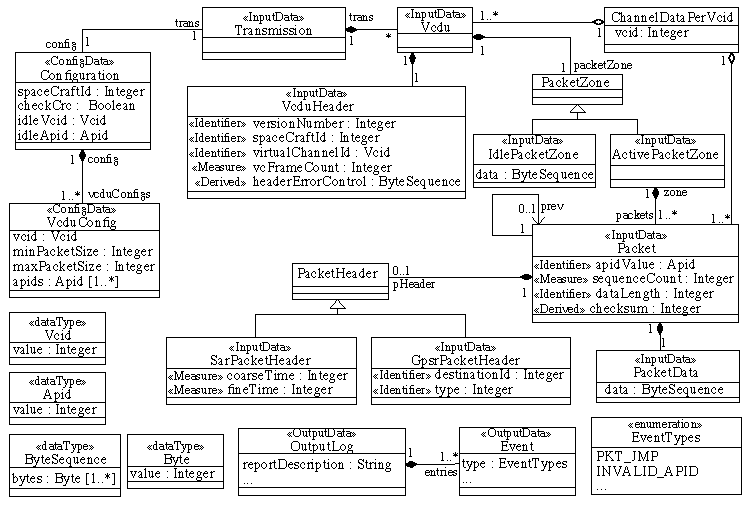
\includegraphics{images/classDiagramSmall}
     \caption{Simplified input data model taken from~\cite{di2015evolutionary}.}
     \label{fig:dataModel}
\end{figure}

Other approaches, instead, work with models specified in formats other than UML class diagrams:
\INDEX{Java classes}~\cite{Boyapati-KORAT-ISSTA-2002,gligoric2010test}, \INDEX{constraint logic}~\cite{Senni-CPLgeneration-TAP-2012}, \INDEX{Alloy}~\cite{Khurshid-SpecificationBasedTesting-ASE-2004}, or \INDEX{Z specifications}~\cite{Horcher-Z-1995}.
These techniques have been proven to be effective for testing software systems that process classical data structures like trees.
Alloy is a modelling language for expressing complex structural constraints~\cite{Jackson:Alloy:2002},
which has been successfully used to generate test inputs for testing object-oriented programs~\cite{Khurshid-SpecificationBasedTesting-ASE-2004}.
Korat, instead, is a technique that enables the generation of data structures to test Java programs~\cite{Boyapati-KORAT-ISSTA-2002}. Given a bound to the input structures (i.e., the maximum number of instances for each class to be used), Korat exhaustively generates all the nonisomorphic structures that are valid.
Some of the limitations of Korat include requiring the definition of an imperative predicate that evaluates the correctness of the generated structure, which could be complex in the case of complex data models, requiring the manual definition of an input bound for each non primitive attribute or association, which might be particularly expensive in case of complex data structure,  not dealing with constraints defined over integers.
A more efficient, black-box test generation approach is UDITA~\cite{gligoric2010test}.
What contributes to the efficiency of UDITA is the combination of both generator methods and predicates.
Generator methods are used to build instances of the data structure, while predicates are used to validate the generated instances. UDITA relies upon the Java Path Finder model checker~\cite{Visser-JPF-2004} to generate all the instances that satisfy the given predicates. However, the implementation of these generator methods that define the complete structure of a complex data model instance and lead to realistic test inputs can be quite expensive.

A common limitation of solutions based on constraint-solvers is their scalability~\cite{di2017augmenting}. In the context of mutation testing, where existing test inputs are available, a possible solution to address the scalability problem may consist of generating new test inputs by \EMPH{regenerating only portions of existing test inputs}.
For example, Di Nardo et al.~\cite{di2017augmenting} automatically generate test inputs for new requirements by adapting existing field data.
This is achieved by combining model transformations with constraint solving.
%% as shown in Fig.~\ref{fig:DiNardo}.
%Model transformations enable the partial reuse of existing field data, while constraint solving allows for the generation of missing data. The approach requires a model of the structure of the data provided by using an UML class diagram with OCL expressions capturing the constraints among data fields. In the case of Di Nardo et al., the missing data correspond to new data types and constraints introduced after updating the requirements of the software under test. In the context of mutation testing, these may correspond to data types not observed during the execution of the test suite.
%In Step 1, a chunk of data is loaded in memory as an instance of the original data model (Original Model Instance).
%A dedicated parser is used for that purpose.
%In Step 2, a model transformation applied to the Original Model Instance is used to generate an instance of the Updated Data Model. The result is an instance of the Updated Data Model that is incomplete (Incomplete Model Instance).
%It contains only the information that can be directly derived from the Original Model Instance:
%instances of classes and attributes that have been introduced in the Updated Data Model are missing from the Incomplete Model Instance (these instances are the ones generated in the next steps of the algorithm).
%In Step 3, UML2Alloy~\cite{Uml2alloy} is used to generate an Alloy model that corresponds to the class diagram and the OCL constraints of the data model; the Alloy Analyzer~\cite{AlloyWeb} is then used to generate  valid instances of the updated data model by means of constraint solving.
%Finally, in Step 4, to generate the concrete test inputs to be processed by the software under test (e.g. a binary file), the content of the Valid Model Instance is written in the format processed by the software under test through a dedicated encoder.
Despite empirical results show a huge performance gain with respect to traditional constraint-based approaches, the need for dedicated parsers to translate existing test inputs into class diagram instances may limit the applicability of the approach. Also, the available test inputs may not enable the generation of all the inputs data needed.

%\begin{figure}[t!]
%  \centering
%    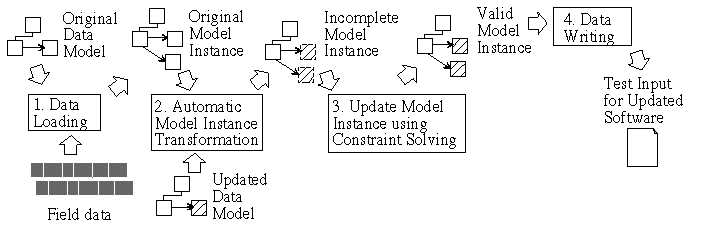
\includegraphics{images/DiNardoTOSEM}
%      \caption{Automatic generation of test inputs for new data requirements proposed by Di Nardo et al~\cite{di2017augmenting}.}
%      \label{fig:DiNardo}
%\end{figure}

Other approaches address the scalability problem by relying on \INDEX{hybrid input generation approaches}~\cite{soltana2019practical}.
For example, PLEDGE~\cite{soltana2019practical} combines metaheuristic search and Satisfiability Modulo Theories (SMT~\cite{SMT:2011}) to generate UML instance models from UML class diagrams annotated with OCL constraints. It  works by using the Negation Normal Form (NNF~\cite{NNF:2001}) to represent all the constraints derived from the UML data model. Different subformulas that build the NNF formula are then solved by combining metaheuristic search and SMT. Metaheuristic search is used to handle subformulas whose satisfaction involves structural tweaks to the instance model, i.e., additions and deletions of objects and links. SMT is used with subformulas involving only primitive attributes, i.e., attributes with primitive types.


When the data exchanged on the communication layer targeted by mutation is the result of a transformation of the input data, the only applicable solution consist in the application of approaches that generate inputs from scratch. By generating a large number of inputs that include instances for all the classes of the data model, these approaches may, in principle, lead to the generation of required data by internal components. However, without means to drive the generation of such data, the application of UML-based test input generation approaches in these situation is likely to be inefficient.

%Despite this approach enables efficient generation of test inputs from scratch, it may still require dedicated parsers for the con

\subsection{Grammars}

When grammars are used to model the input, \INDEX{grammar-based test input generation} approaches relying on the expansion of the production rules of the grammar can be adopted~\cite{fuzzingbook2019:GrammarFuzzer}.
Available tools are shown in Table~\ref{table:grammarGeneration}.

%Listing~\ref{TestJSON} shows the inputs generated by \emph{Coverage-based Fuzzer}~\cite{fuzzingbook2019:GrammarFuzzer} to cover all the production rules and terminals of the grammar (one input per line). Listing~\ref{TestJSON} shows that these automatically generated inputs are difficult to read. For example, for a human, is more difficult to  read Listing~\ref{TestJSON}  than Listing~\ref{JSONfile}.
%
%% !TEX root = ../MutationTestingSurvey.tex
\begin{minipage}{14cm}
\footnotesize
\begin{lstlisting}[caption=Test Cases covering the JSON grammar shown in Listing~\ref{JSONgrammar}, label=TestJSON]
 true 
 null 
 false 
 { "k" : [ "o9*i`BM+Lw^jY7EUyX3e_}(1~$TJS2carZVND@zfh5%qObgu<;K CFW=dm&.[:)xl#'{H8I|]GAQPn,6-v>t0p?s4R!k/tOr" ] } 
 -20.538 
 [ ] 
 { } 
 -7e+9 
 6.13E4 
 90E-008 
 { "" : [ true ] , "" : false , "" : true , "" : true , "" : true } 
 [ [ false ] , true ] 
\end{lstlisting}
\end{minipage}

\begin{table}[h]
\caption{List of tools for grammar-based inputs generation.}
\label{table:grammarGeneration}
\begin{center}
\tiny
\begin{tabular}{|p{2cm}|p{2cm}|p{2cm}|p{7cm}|}
\hline
\textbf{Name}&\textbf{Grammar}&\textbf{Licence}&\textbf{Description}\\
\hline
GramTest~\cite{GramTest}& BNF&Apache 2.0&Java-based tool that allows you to generate test cases based on BNF grammars. It covers all the production rules of the grammar.\\
\hline
Fuzzingbook Grammar Coverage-based Fuzzer~\cite{fuzzingbook2019:GrammarFuzzer}& BNF & MIT &Python tool that implements production rules coverage. It implements the Shortest Path Selection~\cite{Burkhardt:TestFromSyntax} optimization.\\
\hline
GP~\cite{GPlib,Kifetew:GBTest:2017}& Annotated BNF & Proprietary& Tool for the automated generation of inputs from Stochastic Context Free Grammars. Implemented on top of genetic programming algorithms. https://selab.fbk.eu/kifetew/downloads/gplib-607.jar\\
RIDDLE~\cite{ghosh1998testing}&BNF& Proprietary& Tool that adopts a grammar to describe the format of inputs; based on the grammar, random and boundary values are generated for tokens representing input parameters.\\
\hline
\end{tabular}
\end{center}
\end{table}%

Among existing approaches, \INDEX{Parser-Directed Fuzzing} (hereafter, \emph{pFuzzer}) aims at producing valid inputs for input parsers~\cite{mathis2019parser}. The challenge is to cover all the lexical and syntactical features of a certain language. The approach systematically produces inputs for the parser and tracks all the comparisons made; after every rejection, it satisfies the comparisons leading to rejections, effectively covering the input space.
Evaluated on five subjects, from CSV files to JavaScript, the \emph{pFuzzer} prototype covers more tokens than both lexical-based (AFL) and constraint-based approaches (KLEE).


Similarly to the case of UML-based test case generation approaches that generate inputs from scratch, these grammar-based approaches can be adopted when the communication layer targeted by mutation testing is either the input layer or an internal layer.However, they may suffer of inefficiency problems; in additions, grammar can be unlikely used to model the types of data processed by space software.

%\cite{grammar:survey}

\subsection{Block-models}

Among the existing toolsets based on block-models, \INDEX{Peach} is the only one which supports the automated generation of test data. However, it's implementation simply generates random data, the process is referred to as
\INDEX{blind fuzzing}\footnote{https://wiki.mozilla.org/Security/Fuzzing/Peach$\#$Creating\_a\_Data\_Model}.


\subsection{No models}


The generation of test inputs without the need of data model is typically driven by code coverage. A representative solution is given by AFL.
% which has been introduced in Section~\ref{sec:data_operators}.

More in general, approaches that address the problem of automatically testing programs that process structured data can be adopted for this purpose~\cite{Kiran:2008,Braione:2017,Braione:2018}. For example, SUSHI~\cite{Braione:2018} is a tool that aims to cover test objectives that depend on non-trivial data structure instances.
It relies on symbolic execution to generate path conditions that capture the relationship between program paths and input data structures. The path conditions are then translated into fitness functions to enable testing based on meta-heuristic search. A solution for the search problem is a sequence of method invocations that instantiates the structured inputs to exercise the program paths identified by the path condition.

\subsection{Automated Generation of Test Oracles}
\label{sec:oracles:dataMutation}

In the case of data-driven mutation testing, solutions for the \INDEX{automated generation of oracles} that consist of assertions verifying the output of the software under test (see Section~\ref{sec:oraclesGeneration:codeDriven}) might still be applied. However, considering that data-driven mutation testing is more likely adopted in the context of system-level testing, where inputs consist of complex, structured data, the generation of test oracles using techniques built for unit testing is likely infeasible in this context.

Possible solutions may consist of approaches that verify the correctness of the log files generated during the execution of the program~\cite{Pastore:ISSRE:08,Pastore:TKT:17}.
Given a set of log files (or execution traces) generated during valid executions, these approaches can derive \INDEX{finite state automata} (FSAs) that capture the sequences of events and data-flow observed in valid executions. The derived FSAs can be used to verify if new executions match the inferred models. More precisely, they enable the automated detection of invalid sequences of events and data-flows. Despite none of these approaches had been applied in the context of data-driven mutation testing, traces collected from multiple runs of a same test case might be used to derive an FSA that captures the behaviour of a single test case. By relying on multiple traces collected from a same test case we can leverage the generalization power of the inference engines used to generate the FSAs; these inference engines, for example, can automatically recognize and filter out variable elements such as timestamps. The inferred FSAs could thus then be used as oracles for newer executions of the generated test cases. Such approaches have shown to be effective in detecting both functional failures~\cite{Pastore:ISSRE:08} and performance problems~\cite{Pastore:TKT:17}.




% !TEX root = MAIN.tex

\chapter{The FAQAS approach}
\label{chapter:approach}

This chapter presents the theory and the methodology behind the toolset implemented by FAQAS.




% !TEX root =  Main.tex
\section{Code-driven Mutation Analysis: MASS}
\label{ch:mass:approach}

\subsection{Overview}
\label{sec:approach}

\begin{figure}[tb]
\begin{center}
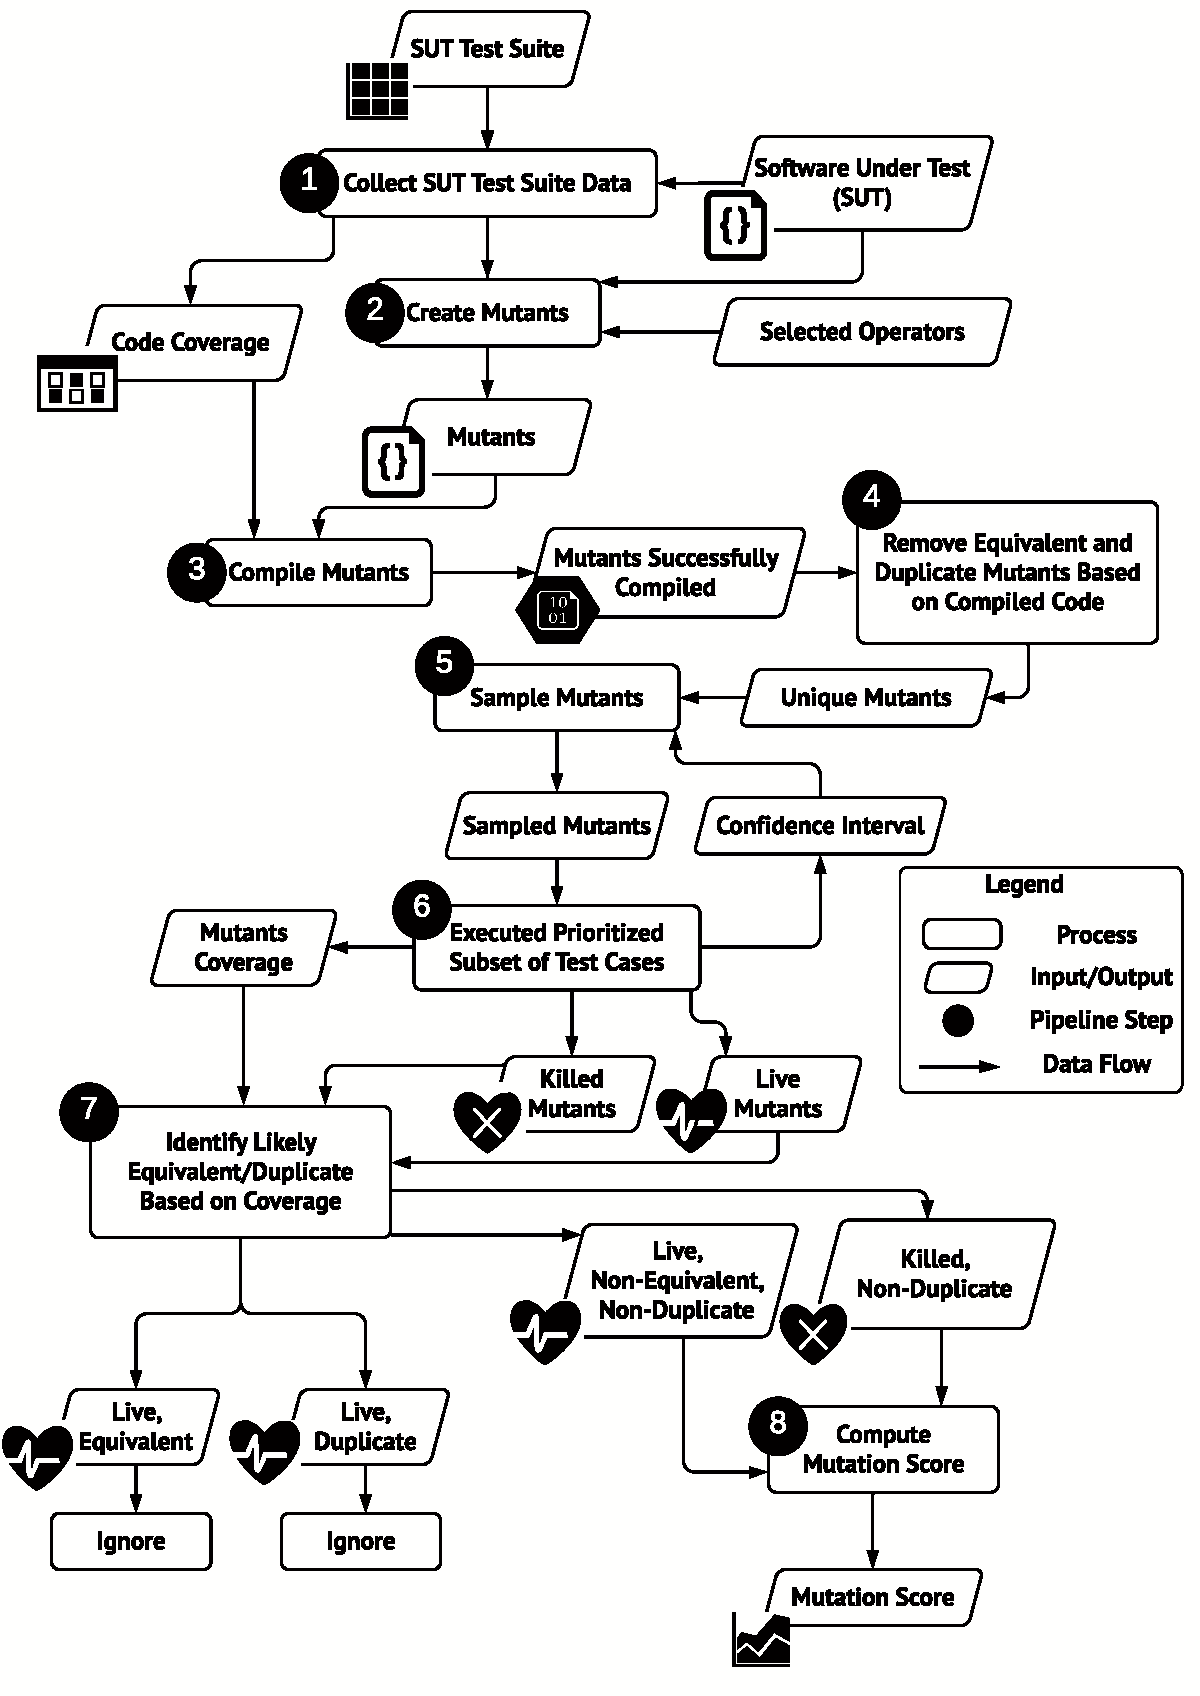
\includegraphics[width=0.6\textwidth]{images/Approach}
\caption{Overview of MASS}
\label{fig:approach}
\end{center}
\end{figure}

Figure~\ref{fig:approach} provides an overview of the mutation analysis process that we propose, \emph{Mutation Analysis for Space Software (\APPR)}. Its goal is to propose a comprehensive solution for making mutation analysis applicable to embedded software in industrial cyber-physical systems. \JMR{3.4}{The ultimate goal of \APPR is to assess the effectiveness of test suites with respect to detecting violations of functional requirements.}
 
\JMR{3.3}{Different from the mutation analysis pipeline presented in related work~\cite{papadakis2019mutation}, \APPR enables the integration of all mutation analysis optimization techniques that are feasible in our context to address scalability and pertinence problems (see Section~\ref{sec:back:summary}). 
\APPR consists of eight steps: (Step 1) Collect SUT Test Suite Data, (Step 2) Create Mutants, (Step 3) Compile Mutants, (Step 4) Remove Equivalent and Duplicate Mutants Based on Compiled Code, (Step 5) Sample Mutants,  (Step 6) Execute Prioritized Subset of Test Cases, 
(Step 7) Identify Likely Equivalent / Duplicate mutants Based on Coverage, and
(Step 8) Compute the Mutation Score. Different from related work, \APPR enables FSCI-based sampling by iterating between mutants sampling (Step 5) and test cases execution (Step 6). 
Also, it integrates test suite prioritization and reduction (Step 6) before the computation of the mutation score.
Finally, it includes methods to identify likely equivalent and duplicate mutants based on code coverage (Step 7).}
We describe each step in the following paragraphs. 

\clearpage
\subsection{Step 1: Collect SUT Test Data}

In Step 1, the test suite is executed against the SUT 
%software under test (SUT) 
and code coverage information is collected. 
More precisely, we rely on the combination of gcov~\cite{GCOV}
and GDB~\cite{GDB}, enabling the collection of coverage information for embedded systems without a file system~\cite{THANASSIS}.
% and Vector CAST~\cite{VectorCAST} 
%to record the number of times each line of code of the SUT has been exercised by a test case.

\subsection{Step 2: Create Mutants}

In Step 2, we automatically generate mutants for the SUT by relying on a set of selected mutation operators.
In \APPR, we rely on an extended sufficient set of mutation operators, which are listed in Table~\ref{table:operators}.
%In addition, in our experiments, we also evaluate the feasibility of relying only on the SDL operator, combined or not with OODL operators, instead of the entire sufficient set of operators.

% !TEX root =  ../Main.tex

\newcommand{\op}{\mathit{op}}
\newcommand{\ArithmeticSet}{ \texttt{+}, \texttt{-}, \texttt{*}, \texttt{/}, \texttt{\%} }
\newcommand{\LogicalSet}{ \texttt{&&}, \texttt{||} }
\newcommand{\RelationalSet}{ \texttt{>}, \texttt{>=}, \texttt{<}, \texttt{<=}, \texttt{==}, \texttt{!=} }
\newcommand{\BitWiseSet}{ \texttt{\&}, \texttt{|}, \land }
\newcommand{\ShiftSet}{ \texttt{>>}, \texttt{<<} }


\begin{table}[h]
\caption{Implemented set of mutation operators.}
\label{table:operators} 
\centering
\scriptsize
\begin{tabular}{|@{}p{4mm}@{}|@{}p{2cm}@{\hspace{1pt}}|@{}p{11.1cm}@{}|}
\hline
&\textbf{Operator} & \textbf{Description$^{*}$} \\
\hline
\multirow{7}{*}{\rotatebox{90}{\emph{Sufficient Set}}}&ABS               & $\{(v, -v)\}$	\\
\cline{2-3}
&AOR               & $\{(\op_1, op_2) \,|\, \op_1, \op_2 \in \{ \ArithmeticSet \} \land \op_1 \neq \op_2 \} $       \\
&    			  & $\{(\op_1, \op_2) \,|\, \op_1, \op_2 \in \{\texttt{+=}, \texttt{-=}, \texttt{*=}, \texttt{/=}, \texttt{\%} \texttt{=}\} \land \op_1 \neq \op_2 \} $       \\
\cline{2-3}
&ICR               & $\{i, x) \,|\, x \in \{1, -1, 0, i + 1, i - 1, -i\}\}$           \\
\cline{2-3}
&LCR               & $\{(\op_1, \op_2) \,|\, \op_1, \op_2 \in \{ \texttt{\&\&}, || \} \land \op_1 \neq \op_2 \}$            \\
&				  & $\{(\op_1, \op_2) \,|\, \op_1, \op_2 \in \{ \texttt{\&=}, \texttt{|=}, \texttt{\&=}\} \land \op_1 \neq \op_2 \}$            \\
&				  & $\{(\op_1, \op_2) \,|\, \op_1, \op_2 \in \{ \texttt{\&}, \texttt{|}, \texttt{\&\&}\} \land \op_1 \neq \op_2 \}$            \\
\cline{2-3}
&ROR               & $\{(\op_1, \op_2) \,|\, \op_1, \op_2 \in \{ \RelationalSet \}\}$            \\
&				  & $\{ (e, !(e)) \,|\, e \in \{\texttt{if(e)}, \texttt{while(e)}\} \}$ \\
\cline{2-3}
&SDL               & $\{(s, \texttt{remove}(s))\}$            \\
\cline{2-3}
&UOI               & $\{ (v, \texttt{--}v), (v, v\texttt{--}), (v, \texttt{++}v), (v, v\texttt{++}) \}$            \\   
\hline
\hline
\multirow{5}{*}{\rotatebox{90}{\emph{OODL}}}&AOD               & $\{((t_1\,op\,t_2), t_1), ((t_1\,op\,t_2), t_2) \,|\, op \in \{ \ArithmeticSet \} $       \\ 
\cline{2-3}
&LOD               & $\{((t_1\,op\,t_2), t_1), ((t_1\,op\,t_2), t_2) \,|\, op \in \{  \} \}$       \\ 
\cline{2-3}
&ROD               & $\{((t_1\,op\,t_2), t_1), ((t_1\,op\,t_2), t_2) \,|\, op \in \{ \RelationalSet \} \}$       \\ 
\cline{2-3}
&BOD               & $\{((t_1\,op\,t_2), t_1), ((t_1\,op\,t_2), t_2) \,|\, op \in \{ \BitWiseSet \} \}$       \\ 
\cline{2-3}
&SOD               & $\{((t_1\,op\,t_2), t_1), ((t_1\,op\,t_2), t_2) \,|\, op \in \{ \ShiftSet \} \}$       \\ 
%\hline
%COR               & $\{(\op_1, \op_2) \,|\, \op_1, \op_2 \in \{ \texttt{\&\&}, \texttt{||}, \land \} \land \op_1 \neq \op_2 \}$            \\
\hline
\hline
\multirow{3}{*}{\rotatebox{90}{\emph{Other}}}&LVR			& $\{(l_1, l_2) \,|\, (l_1, l_2) \in \{(0,-1), (l_1,-l_1), (l_1, 0), (\mathit{true}, \mathit{false}), (\mathit{false}, \mathit{true})\}\}$\\
&&\\
&&\\
\hline
\end{tabular}

$^{*}$Each pair in parenthesis shows how a program element is modified by the mutation operator. Th eleft element of the pair is replaced with the right element. We follow standard syntax~\cite{kintis2018effective}. Program elements are literals ($l$), integer literals ($i$), boolean expressions ($e$), operators ($\op$), statements ($s$), variables ($v$), and terms ( $t_i$, which might be either variables or literals).
\end{table}

%To automatically generate mutants, we have extended SRCIRor~\cite{hariri2018srciror} to include all the 
%operators in Table~\ref{table:operators}. 
%After mutating the original source file, our extension saves the mutated source file and keeps track of the mutation applied. Our toolset is available under the ESA Software Community Licence Permissive~\cite{ESAlicence} at the following URL \textbf{https://faqas.uni.lu/}.

\subsection{Step 3: Compile mutants}
\label{sec:appr:compile}

In Step 3, we 
compile mutants by relying on an optimized compilation procedure that leverages the build system of the SUT. To this end, we have developed a toolset that, for each mutated source file: (1) backs-up the original source file, (2) renames the mutated source file as the original source file, (3) runs the build system (e.g., executes the command \texttt{make}), (4) copies the generated executable mutant in a dedicated folder, (5) restores the original source file. Mutants that lead to compilation errors are discarded.

%Build systems \JMR{1.15}{(e.g., GNU make~\cite{MAKE} driving the GCC~\cite{GCC} compiler)} create one object file for each source file to be compiled and then link these object files together into the final executable. 
%\CHANGED{After the first build, in subsequent builds, 
%build systems
%%they 
%recompile only the modified files and link them to the rest.}
%For this reason, our optimized compilation procedure, which modifies at most two source files for each mutant (i.e., the mutated file and the file restored to eliminate the previous mutation), can reuse almost all the compiled object files in subsequent compilation runs, thus speeding up the compilation of multiple mutants. The experiments conducted with our subjects have shown that 
%%additional optimizations are not necessary to make the compilation of mutants feasible.
%\CHANGED{our optimization is sufficient to make the compilation of mutants feasible for large projects. Other state-of-the-art solutions introduce additional complexity (e.g., change the structure of the software under test~\cite{untch1993mutation}) that does not appear to be justified by scalability needs.}
 
% Concerning compilation warnings, we assume the build system of the SUT has been properly configured; more precisely, if the system should compile without warnings, the compiler is expected to be configured to treat warnings as errors otherwise mutants that lead to warning are retained.}

\subsection{Step 4: Remove equivalent and redundant mutants based on compiled code}

In Step 4, we rely on trivial compiler optimizations to identify and remove equivalent and redundant mutants. 
\REVNOV{C-P-15}{We compile the original software and every mutant multiple times once for each every available optimization option (i.e., \texttt{-O0}, \texttt{-O1}, \texttt{-O2}, \texttt{-O3}, \texttt{-Os}, \texttt{-Ofast} in GCC) or a subset of them.
After each execution of the compiler, we compute the SHA-512 hash summary of the generated executable.}To detect equivalent mutants, \APPR compares the hash summaries of the mutants with that of the original executable. To detect duplicate mutants but avoid combinatorial explosion, \APPR focuses its comparison of hash summaries on pairs of mutants belonging to the same source file (restricting the scope of the comparison is common practice~\cite{kintis2017detecting}).
Hash comparison allows us to (1) determine the presence of equivalent mutants (i.e., mutants having the same hash as the original executable), and (2) identify duplicate mutants (i.e., mutants with the same hash). %Mutants that are identified as being either equivalent and duplicate mutants are ignored in the following steps of \APPR. 
Equivalent and duplicate mutants are then discarded. 

%We compare hash summaries rather than executable files because it is much faster, an important consideration when dealing with a large number of mutants.
%The outcome of Step 4 is a set of \INDEX{unique mutants}, i.e., mutants with compiled code that differs from the original software and any other mutant.


\subsection{Step 5: Sample Mutants}
\label{sec:codeDriven:samplingStep}
\STARTCHANGEDNOV


In Step 5, \APPR samples the mutants to be executed to compute the mutation score. 
\JMR{1.8 3.3}{\APPR does not selectively generate mutants but samples them from the whole set of successfully compiled, nonequivalent, and nonduplicated mutants (result of Steps 2 to 4). This choice aims to avoid sampling bias which may result from the presence of such mutants; indeed, there is no guarantee that these mutants, if they were discarded after being sampled, would be uniformly distributed across program statements. Our choice does not affect the feasibility of \APPR since Steps 2 to 4 have negligible cost.}

Our pipeline supports different sampling strategies: \INDEX{proportional uniform sampling}, \INDEX{proportional method-based sampling},  \INDEX{uniform fixed-size sampling}, and \INDEX{uniform FSCI sampling}, which is an innovative contribution of the FAQAS actvity~\cite{Oscar:MASS:TSE}. 

%The strategies \INDEX{proportional uniform sampling} and \INDEX{proportional method-based sampling} were selected based on the results of Zhang et al.~\cite{zhang2013operator}, who compared eight strategies for sampling mutants. 
%The former was the best performing strategy and consists of sampling mutants evenly across all functions of the SUT, i.e., sampling $r\%$ mutants from each set of mutants generated inside the same function.
%The latter consists of randomly selecting $r\%$ mutants from the complete mutants set. This is included in our study because it is simpler to implement and showed to be equivalent to stratified sampling strategies, based on recent work~\cite{gopinath2015hard}.
%
%The \INDEX{uniform fixed-size sampling} strategy stems from the work of Gopinath et al.~\cite{gopinath2015hard} and consists of selecting a fixed number $N_M$ of mutants for the computation of the mutation score. Based their work, with 1,000 mutants, one can guarantee an accurate estimation of the mutation score.
%% In our empirical evaluation, we assess the accuracy obtained for $N_M$ values across the range [100;1000].}
%
%In this paper, we introduce the \INDEX{uniform FSCI sampling} strategy that determines the sample size dynamically, while exercising mutants, based on a fixed-width sequential confidence interval approach.
%With \INDEX{uniform FSCI sampling}, we introduce a cycle between Step 6 and Step 5, such that a new mutant is sampled only if deemed necessary.
%% of the mutation testing results collected so far. 
% More precisely, \APPR iteratively selects a random mutant from the set of unique mutants and exercises it using the SUT test suite. 
%% The result of each mutant execution (i.e., killed or live) is treated as a Bernoulli trial that is used to compute the confidence interval according to the FSCI method. 
%Based on related work, we assume that the mutation score computed with a sample of mutants follows a binomial distribution (see Section~\ref{sec:scalability}).
%For this reason, to compute the confidence interval for the FSCI analysis, we rely on the Clopper-Pearson method since it is reported to provide the best results (see Section~\ref{sec:scalability}).
%Mutation analysis (i.e., sampling and testing a mutant) stops when the confidence interval is below a given threshold $T_{\mathit{CI}}$ (we use $T_{\mathit{CI}}=0.10$ in our experiments). More formally, given a confidence interval 
%$[\mathit{L}_{S};\mathit{U}_{S}]$, with $\mathit{L}_{S}$ and $\mathit{U}_{S}$ indicating the lower and upper bound of the interval, mutation analysis stops when the following condition holds:
%\begin{equation}
%\label{eq:CI:T}
%(\mathit{U}_{S}-\mathit{L}_{S})<T_{\mathit{CI}}.
%\end{equation}
%
%Unfortunately, the assumption about the estimated mutation score following a binomial distribution may not hold when a subset of the test suite is executed for every mutant (which could happen in Step 6). Without going into the details behind the implementation of Step 6, which is described in Section~\ref{sec:step:prioritize}, 
%we can expect that a reduced test suite may not be able to kill all the mutants killed by the entire test suite, i.e., the estimated mutation score may be affected by negative bias. Consequently, over multiple runs, the mean of the estimated mutation score may not be close to the \INDEX{actual mutation score} (i.e., the mutation score computed with the entire test suite exercising all the mutants for the SUT)
% but may converge to a lower value. 
%To compute a correct confidence interval that includes the actual mutation score of the SUT, we thus need to take into account this negative bias.
%
%To study the effect of negative bias on the confidence interval, we address first the relation between the actual mutation score and the mutation score computed with the reduced test suite when the entire set of mutants for the SUT is executed. 
%A mutant killed by the entire test suite has a probability $P_{\mathit{KErr}}$ of not being killed by the reduced test suite.
%The probability $P_{\mathit{KErr}}$  can be estimated as the proportion of mutants (erroneously) not killed by the reduced test suite 
%\begin{equation}
%P_{\mathit{KErr}} = \frac{|E_R|}{|M|}
%\end{equation}
%with 
%$E_R$ being the subset of mutants that are killed by the entire test suite but not by the reduced test suite, and $M$ being the full set of mutants for the SUT.
%
%The mutation score for the reduced test suite ($\mathit{MS}_R$) can be computed as
%
%\begin{equation}
%\small
%\mathit{MS}_R=\frac{|K|-|E_R|}{|M|}=\frac{|K|}{|M|}-\frac{|E_R|}{|M|}=\mathit{MS}-\frac{|E_R|}{|M|}=\mathit{MS}-P_{\mathit{KErr}}
%\end{equation}
%
%where $K$ is the set of mutants killed by the whole test suite, $M$ is the set of all the mutants of the SUT,  and $\mathit{MS}$ is the actual mutation score. Consequently, the actual mutation score can be computed as 
%\begin{equation}
%\label{eq:MS}
%\mathit{MS}=\mathit{MS}_R+P_{\mathit{Err}_R}
%\end{equation}
%
%We now discuss the effect of a reduced test suite on the confidence interval for a mutation score estimated with mutants sampling. When mutants are sampled and tested with the entire test suite, the actual mutation score is expected to lie in the confidence interval $[\mathit{L}_{S};\mathit{U}_{S}]$. 
%\CHANGED{In the presence of a reduced test suite, we can still rely on the Clopper-Pearson method to compute the confidence interval $\mathit{CI}_R=[\mathit{L}_{R};\mathit{U}_{R}]$.
%However, }
%%in the presence of a reduced test suite,
%we have to take into account the probability of an error in the computation of the mutation score $\mathit{MS}_R$;  $\mathit{MS}_R$ can be lower than $\mathit{MS}$ and, based on Equation~\ref{eq:MS}, we expect the actual mutation score to lie in 
%%the interval.
%\JMR{NEW}{an interval that is shifted with respect to the interval for $\mathit{MS}_R$:}
%
%\begin{equation}
%\label{eq:CI}
%\mathit{CI}=[\mathit{L}_{R}+P_\mathit{KErr};\mathit{U}_{R}+P_{\mathit{KErr}}]
%\end{equation}
%
%We can only estimate  $P_{\mathit{KErr}}$ since computing it would require the execution of all the mutants with the complete test suite, thus undermining our objective of reducing test executions. 
%To do so, we can randomly select a subset $M_R$ of mutants, on which to execute the entire test suite and identify the mutants killed by the reduced test suite. %\footnote{In our implementation, we record the outcome of each test case of the whole suite and then simulate the execution of the reduced test suite, thus saving time.} 
%The size of the set $M_R$ should be lower than the number of mutants we expect FSCI sampling to return, 
%%(e.g., we use $M_R=100$ in our experiments\footnote{Though it would be possible to also estimate $P_{\mathit{KErr}}$ with FSCI, we leave it for future work.}), 
%otherwise sampling would not provide any cost reduction benefit.
%Since, for every mutant in $M_R$, we can determine if it is erroneously reported as not killed by the reduced test suite R,
%we can 
%%end up with a vector of boolean evaluations $E=e_1, ..., e_n$ where each evaluation $e_i$ is equal to \emph{true} if the $i^{th}$ mutant has been erroneously indicated as not killed by the reduced test suite.
%%This population of evaluations enable us to 
%estimate the probability $P_{\mathit{KErr}}$ as the percentage of such mutants.
%As for the case of the mutation score, 
%%these mutants tend to be positively  correlated\footnote{If a line of code contains a mutant that is not killed by the reduced test suite, it may contain another such mutant.} and, for this reason,
%we assume that the binomial distribution provides a conservative estimate of the variance for $P_{\mathit{KErr}}$. 
%
%We can estimate the confidence interval for $P_{\mathit{KErr}}$ using one of the methods for binomial distributions.
%We rely on the Wilson score method because it is known to perform well with small samples~\cite{Newcombe:Wilson:1998}. 
%The value of $P_{\mathit{KErr}}$ will thus lie within $\mathit{CI}_E=[\mathit{L}_{E};\mathit{U}_{E}]$,  with $\mathit{L}_{E}$ and $\mathit{U}_{E}$ indicating the lower and upper bounds of the interval.
%
%
%
%\NEWFSCI{Based on Equation~\ref{eq:CI}, 
%%to ensure that the actual mutation score lies in the computed confidence interval, we should assume the worst case, i.e., $P_{\mathit{KErr}}=\mathit{U}_{E}$.
%the confidence interval to be used with FSCI sampling in the presence of a reduced test suite should thus be }
%\begin{equation}
%\label{eq:CI:FSCI}
%\mathit{CI}=[\mathit{L}_{R}+\mathit{L}_{E};\mathit{U}_{R}+\mathit{U}_{E}]
%\end{equation}
%
%\JMRCHANGE{The estimated mutation score is the value lying in the middle of the interval.}
%
%\UPDATE{Since the width of the confidence interval CI (hereafter, $|CI|$) results from the sum of $|\mathit{CI}_R|$ and $|\mathit{CI}_E|$,
%%Also, from a practical perspective, \JMRCHANGE{the terms $+\mathit{L}_{E}$ and} $+\mathit{U}_{E}$ may augment the size of the interval returned by the Clopper-Pearson method; consequently, 
%mutation sampling with a reduced test suite may lead to the execution of a larger set of mutants.}
%
%\UPDATE{Based on Equations~\ref{eq:CI:T} and~\ref{eq:CI:FSCI}, $|\mathit{CI}_R| \le T_{\mathit{CI}} - |\mathit{CI}_E|$.
%Consequently, when $|\mathit{CI}_E|>T_{\mathit{CI}}$, the reduced test suite cannot lead to sufficiently accurate results. 
%Also, a large $|\mathit{CI}_E|$ may prevent the identification of accurate results with a feasible number of mutants. For example, Clopper-pearson may require up to 1568 samples for a confidence interval below 0.05~\cite{Goncalves2012}}. 
%%the interval is 3.5, you will need a $[\mathit{L}_{R};\mathit{U}_{R}]$ of 7.5, which may require XXXX samples in the worst case).
%%https://select-statistics.co.uk/calculators/sample-size-calculator-population-proportion/
%%Basic Business Statistics, Global Edition, 13th Edition
%\UPDATE{
%We shall thus identify a threshold ($T_{\mathit{CE}}$) for the confidence interval $|\mathit{CI}_E|$ that enables 
%%$|\mathit{CI}_R| \le (T_{\mathit{CI}} - |\mathit{CI}_E|)$ 
%accurate estimates 
%with a small sample size (e.g., in the worst case, with less than 1000 samples, the sample size for related work).
%For this reason, starting from a minimal number of samples to estimate $P_{\mathit{KErr}}$ (150 in our experiments), \APPR keeps estimating $P_{\mathit{KErr}}$ until it yields $|\mathit{CI}_E| \le T_{\mathit{CE}}$. 
%In our experiments we set $T_{\mathit{CE}} = 0.035$.
%To select $T_{\mathit{CE}}$, we have identified a reasonable minimal mutation score to be expected in space software (i.e., 65\%) and identified, based on confidence interval estimation methods with finite population correction factor~\cite{BasicBusinessStatistics}, 
%the minimal value for $|\mathit{CI}_E|$ that requires a number of samples below 850 (i.e., $1000-150$).
%%Indeed, for a binomial proportion with a probability of success above 65\% (the minimal mutation score), a confidence interval width of 0.065 (i.e., $0.1-0.035$) shall be achieved with a sample size of 821.}
%}
%
%When it is not possible to estimate $|\mathit{CI}_E| \le T_{\mathit{CE}}$ \UPDATE{or when the number of samples required to estimate $|\mathit{CI}_E| \le T_{\mathit{CE}}$ is sufficient to accurately estimate the mutation score,} the test suite can be prioritized but not reduced and the confidence interval is computed using the traditional Clopper-Pearson method, i.e., $[\mathit{L}_{S};\mathit{U}_{S}]$.
%
%
%\ENDCHANGEDNOV

\subsection{Step 6: Execute prioritized subset of test cases}
\label{sec:step:prioritize}

In Step 6, we execute a prioritized subset of test cases. 
We select only the test cases that satisfy 
the reachability condition (i.e., cover the mutated statement) and  execute them in sequence.
Similarly to the approach of Zhang et al. \cite{zhang2013faster}, we define the order of execution of test cases based on their estimated likelihood of killing a mutant.
\CHANGED{However, in our work, this likelihood is estimated differently since, as discussed above, the measurements they rely on are not applicable in the context of system-level testing and complex cyber-physical systems 
(see Section~\ref{sec:scalability}).} \CHANGEDNOV{In contrast, to minimize the impact of measurements on real-time constraints, we only collect code coverage information for a small part of the system.}
%However, we redefined the criteria for the prioritization and selection of test cases because of the inapplicability of the ones proposed by Zhang et al. (see Section~\ref{sec:scalability}).

%However, we notice that such optimization may not be sufficient when test suites are particularly large; indeed, prioritizing test cases may not be sufficient to reduce execution time. For example, live mutants may lead to the execution of a large number of test cases when almost all the test cases of the test suite exercise the mutated statement. 
\REVNOV{C-P-46}{We execute only covered statements assuming that the test suite is optimal with respect to code coverage. More precisely, we addume that if a statement is not covered there is a good reason for it (e.g., it depends on hardware). 
If a statement is not covered by the test suite, there is no chance that a mutant generated in the non-covered statement can be possibly detected by any test case. 
If the test suite does not reach the required coverage there is no reason to perform mutation testing, because is already known that the test suite is not good.}

%To reduce the number of test cases to be executed with a mutant, 
%we should first execute the ones that more likely satisfy the necessity condition. 
%This might be achieved by executing a test case that exercises the mutated statement with variable values not observed before. 
%Unfortunately, in our context, the size of the SUT and its real-time constraints prevent us from recording all the variable values processed during testing. 
%
%Therefore, we rely on code coverage to determine if two test case executions exercise the mutated statement with diverse variable values. Such coverage is collected by efficient procedures provided by compilers, thus having lower impact on execution performance than other types of dynamic analysis solutions (e.g., tracing variable values).
%% as a surrogate indicator of  variable values diversity.
%%diversity in values assigned to the variables used in a statement. 
%Since, because of control- and data-flow dependencies, a different set of input values may lead to differences in code coverage, 
%the latter helps determine if two or more test cases likely exercise a mutated statement with different variable values. %Indeed, a difference in the set of 
%%statements covered by two test cases depends on the values reaching some of the program statements, including the mutated one.
%%Indeed, a difference in the set of 
%%statements covered by two or more test cases that exercise a same mutated statement may depend on the values used in such statement. 
%%For example, the definition of a variable may lead to the execution of different branches when different values are assigned across distinct executions.
%To increase the likelihood that the observed differences in code coverage are due to the use of different variable values to exercise the mutated statement, we restrict the scope of code coverage analysis 
%to the functions belonging to the component (i.e., the source file) that contains the mutated statement.
%%However, two test case executions may also present coverage differences 
%%because of a diverse set of variable values used by statements other than the mutated one. 
%%For this reason, we restrict the scope of code coverage analysis 
%%to the functions belonging to a same component (i.e., a same source file).
%Indeed, such functions typically present several control- and data-flow dependencies, thus 
%augmenting the likelihood that a coverage difference is due to the execution of the mutated statement with a diverse set of values. Also, collecting code coverage for a small part of the system further reduces the impact of our analysis on system performance.
%
%%to the mutated function, its callers, and its callees.
%%to maximize the chances that a change in the behaviour of the software depends on the values used in a mutated statement, we determine that two executions likely exercise a mutated statement with diverse values by focussing on the coverage of 
%%the mutated function, its callers, and its callees.
%%A reduced scope is effective in determining behavioural differences based on the analysis of variable valuations~\cite{Pastore:VART:2014}.
%
%%Since related work focuses on either statement coverage or the frequency of execution of a statement, 
%Based on related work, we have identified two possible strategies to characterize test case executions based on code coverage:
%\begin{itemize}
%\item[S1] Compare the sets of source code statements that have been covered by test cases~\cite{grun2009impact}.
%%\item[C2] Identify the set of unique pairs $\langle\mathit{statement},\mathit{arity}\rangle$, where $\mathit{statement}$ is a unique identifier for the source code statement, and $\mathit{arity}$ is a symbol (i.e., $1$ or $*$) indicating if the statement has been covered one or more times.
%\item[S2] Compare the number of times each statement has been covered by test cases~\cite{schuler2013covering}.
%\end{itemize}
%
%
%To determine how dissimilar two test cases are and, consequently, how likely they exercise the mutated statement with different values, we rely on widely adopted distance metrics. 
%In the case of S1, we rely on the Jaccard and Ochiai index, which are two similarity indices for binary data and have successfully been used to compare program executions based on code coverage~\cite{Zou:Ochiai:2019,Keller:Jaccard:2017,Briand:2019}. 
%\REVNOV{C-P-18}{The Jaccard index is also known as \INDEX{intersection over union} 
%it measures similarity between sets, and is defined as the size of the intersection divided by the size of the union.
%The Jaccard distance measures dissimilarity between sample sets and results from subtracting the Jaccard coefficient from 1.
%The Ochiai index calculates cosine similarity with binary data, it is used in molecular biology and software engineering.}
%Given two test cases $T_A$ and $T_B$, the Jaccard  ($D_J$) and Ochiai ($D_O$) distances are computed as follows:
%
%$D_J(T_a,T_b)=1-\frac{|C_a \cap C_b|}{|C_a \cup C_b|}$ \hspace{2mm} $D_O(T_a,T_b)=1-\frac{|C_a \cap C_b|}{\sqrt{|C_a| * |C_b|}}$, 
%where $C_a$ and $C_b$ are the set of covered statements exercised by $T_a$ and $T_b$, respectively.
%
%In the case of S2, we compute the distance between two test cases by relying on the euclidean distance ($D_E$) and the cosine similarity distance ($D_C$), two popular distance metrics used in machine learning.
%\REVNOV{C-P-18}{Euclidean distance is the straight-line distance between two points in Euclidean space; precisely, the Euclidean distance between two points is the length of the line segment connecting them. In our context, the two vectors consist of the number of times the program statements had been exercised by a test. Cosine similarity measures similarity between two vectors of an inner product space. It results from the inner product of the same vectors normalized to both have length 1, which matches the the cosine of the angle between them. It is widely adopted to measure cohesion within clusters in data mining.}
%Given two vectors $V_A$ and $V_B$, whose elements capture the number of times a statement has been covered by test cases $T_A$ and $T_B$, the distances $D_E$ and $D_C$ can be computed as follows:
%
%$D_E=\sqrt{\sum_{i=1}^{n}(A_i-B_i)^2}$
%
%$D_C= 1-\frac{\sum_{i=1}^{n}A_i*B_i}{\sqrt{\sum_{i=1}^{n}{A_i}^2}*\sqrt{\sum_{i=1}^{n}{B_i}^2}}$,
%%Their main difference is that cosine similarity is used when the magnitude of the vectors should not matter.
%where $A_i$ and $B_i$ refer to the number of times the i-th statement had been covered by $T_A$ and $T_B$, respectively.
%
%Figure~\ref{alg:prioritize} shows the pseudocode of our algorithm for selecting and prioritizing test cases. It generates as output
%a prioritized test suite (\INDEX{PTS}).
%Based on the findings of Zhang et al. \cite{zhang2013faster}, we first select the test case that exercises the mutated statement the highest number of times (Line~\ref{alg:prioritize:first}) \CHANGED{ and add it to the prioritized test suite (Line~\ref{alg:prioritize:add}).}
%Then, in the next iterations, the test case selected is the one with the largest distance from the closest test case already selected (Lines~\ref{alg:prioritize:selectStart} to~\ref{alg:prioritize:selectEnd}). 
%When two or more test cases have the same distance, we select randomly among the test cases that exercise the mutated statement the most.
%%is most different than any other test case already included in the prioritized test suite.
%
%%Then, since we aim to maximize test cases diversity, the next selected test case should be the one that is most different than any other test case already included in the prioritized test suite.
%%For this reason, for each test case $n$ not selected yet (Line~\ref{alg:prioritize:notSel}), we identify the test case $t$ showing the most similar coverage (i.e., the one with the minimal distance $d$, Line~\ref{alg:prioritize:minD}). We then select the test case $n$ with the highest distance from its closest test case (Lines~\ref{alg:prioritize:selectStart} to~\ref{alg:prioritize:selectEnd}). 
%
%The algorithm iterates as long as it identifies a test case
%showing a difference in code coverage from the 
%%that exercises 
%%the program statements differently than 
%already selected test cases (Line~\ref{alg:prioritize:until}).
%
%Test cases are then executed in the selected order. During  execution, we collect code coverage information and identify killed and live mutants.
%
%
%% !TEX root =  ../Main.tex

\newcommand{\INDA}{10}
\newcommand{\INDB}{15}
\newcommand{\INDC}{5}

%\vspace{-3mm}
\begin{figure}[tb]

\begin{algorithmic}[1]

%\footnotesize
\scriptsize
\Require \emph{TS}, the test suite of the software under test
\Require \emph{Cov}, coverage information, for each test case
\Require \emph{ms}, the mutated statement
\Ensure \emph{PTS}, a list of test cases to be executed, sorted by priority
% (source inputs, follow-up inputs, output data).

\State $\mathit{TS}_m \gets$ subset of $\mathit{TS}$ that cover the mutated statement $\mathit{ms}$, based on \emph{Cov} \label{alg:prioritize:select}
\State $\mathit{PTS} \gets \mathit{new} \mathit{list}$ \textcolor{darkgray}{//this list is initially empty}
\State $\mathit{PTS} \gets$ based on \emph{Cov} select from $\mathit{TS_m}$ the test case $t$ that exercises $\mathit{ms}$ more times \label{alg:prioritize:first}
\State $\mathit{PTS} \gets \mathit{PTS} \cup t$ \textcolor{darkgray}{//include first the test case selected above}  \label{alg:prioritize:add}

\State \textbf{repeat} \label{alg:prioritize:repeat}
\State \hspace{\INDC mm} \textbf{for each} $n$ in the set ($\mathit{TS}_m$ - $\mathit{PTS}$) \textcolor{darkgray}{, which is the set of test cases not already added to $\mathit{PTS}$} \label{alg:prioritize:notSel}
\State \hspace{\INDA mm} \textbf{for each} $t$ in $\mathit{PTS}$
\State \hspace{\INDB mm} compute the distance between $t$ and $n$
\State \hspace{\INDA mm} identify $t_n$ i.e., the test case $t$ with the minimal $d$ \label{alg:prioritize:minD}
\State \hspace{\INDC mm} among all the $t_n$ identified, select the one with the highest distance $d$ \label{alg:prioritize:selectStart}
\State \hspace{\INDC mm} \textbf{if} $d > 0$ \textcolor{darkgray}{//there is at least a test case with a different coverage}
\State \hspace{\INDA mm} \textcolor{darkgray}{//note: $n$ is the test case in the set ($\mathit{TS}_m$ - $\mathit{PTS}$) closer to $t_n$}
\State \hspace{\INDA mm} $\mathit{PTS} \gets \mathit{PTS} \cup n$ \label{alg:prioritize:selectEnd}
\State \textbf{until} $d > 0$ \label{alg:prioritize:until}


\end{algorithmic}
\vspace{-3mm}
\caption{Algorithm for prioritizing test cases}
%\vspace{-0.2cm}
\label{alg:prioritize}
\end{figure}




\subsection{Step 7: Discard Mutants}
\label{sec:algostepSeven}


In this step, we identify likely nonequivalent and likely nonduplicate mutants by relying on code coverage information \CHANGED{collected in the previous step}.

Similarly to related work~\cite{schuler2013covering}, 
%since the size of a program may determine the degree of non-determinism in statement coverage, 
we identify nonequivalent and nonduplicate mutants based on a threshold.

In our case, consistently with previous steps of \APPR,
we compute normalized distances based on the distance metrics $D_J$, $D_O$, $D_E$, and $D_C$. A mutant is considered nonequivalent when the distance from the original program is above the threshold $T_E$, for at least one test case.
Similarly, a mutant is considered nonduplicate when the distance from every other mutant is above the threshold $T_D$, for at least one test case. For the identification of nonequivalent mutants, we consider live mutants only. To identify nonduplicate mutants, we consider both live and killed mutants; however, to avoid combinatorial explosion, we compare only mutants belonging to the same source file (indeed, mutants belonging to different files are unlikely to be redundant). 
Killed mutants that lead to the failure of different test cases are not duplicate, regardless of their distance.

Thresholds $T_E$ and $T_D$ should enable the identification of mutants that are guaranteed to be nonequivalent and nonduplicate. In particular, we are interested in the set of \emph{live, nonequivalent, nonduplicate mutants} (hereafter, $\mathit{LNEND}$) and the set of \emph{killed, nonduplicate mutants} (hereafter, $\mathit{KND}$). With such guarantees, the mutation score can be adopted as an adequacy criterion in safety certification processes. For example, certification agencies may require safety-critical software to reach a mutation score of 100\%, which is feasible in the presence of nonequivalent mutants. 
%This will enable the adoption of mutation score as an adequacy criterion, 

%\REVNOV{C-P-19}{Figure~\ref{alg:nonEquivalent:nonRedeundat} shows the algorithm for detecting nonequivalent and nonduplicate mutants.
%It first identify among the list of killed mutants all the non-duplicate ones (Line~\ref{alg:equivalent:KND}).
%Then it identifies the non-equivalent mutants among the list of live mutants (Line~\ref{alg:equivalent:LNE}).
%Finally, it further filters the list of non-equivalent mutants to keep only the ones that appear to be nonduplicate (Line~\ref{alg:equivalent:LNEND}).}
%
%% !TEX root =  ../Main.tex

\renewcommand{\INDA}{5}
\renewcommand{\INDB}{10}
\renewcommand{\INDC}{15}
\newcommand{\INDD}{20}
\newcommand{\INDE}{25}

\renewcommand{\Comment}[1]{\textcolor{darkgray}{\textit{//#1}}}

%\vspace{-3mm}
\begin{figure}[tb]

\begin{algorithmic}[1]

%\footnotesize
\scriptsize
\Require \emph{D}, the distance function to use to identify equivalent/duplicate mutants
\Require \emph{KM}, list of killed mutants
\Require \emph{LM}, list of live mutants
\Require $\mathit{Cov}_O$, coverage information for all the test cases, for the original program
\Require $\mathit{Cov}_M$, coverage information for all the executed test cases, for every mutant
\Require \emph{TS}, list of test cases
\Require \emph{TR}, test results, for all the executions
\Ensure \emph{KNR}, a list of killed, non-duplicate  mutants
\Ensure \emph{LNENR}, a list of live, non-equivalent, non-duplicate mutants
% (source inputs, follow-up inputs, output data).

%\State $\mathit{TS}_m \gets$ subset of $\mathit{TS}$ that cover the mutated statement $\mathit{ms}$, based on \emph{Cov} \label{alg:equivalent:select}
%\State $\mathit{PTS} \gets \mathit{new} \mathit{list}$ \textcolor{darkgray}{//this list is initially empty}
%\State $\mathit{PTS} \gets$ based on \emph{Cov} select from $\mathit{TS_m}$ the test case $t$ that exercises $\mathit{ms}$ more times \label{alg:equivalent:first}
\State $\mathit{KNR} \gets \mathit{identifyNonDuplicateMutants(} \mathit{KM}, \mathit{TS}, \mathit{TR}, \mathit{Cov}_M)$ \label{alg:equivalent:KNR}
\State $\mathit{LNE} \gets \mathit{identifyNonEquivalentMutants(} \mathit{LNR}, \mathit{TS}, \mathit{Cov}_M, \mathit{Cov}_O)$ \label{alg:equivalent:LNE}
\State $\mathit{LNENR} \gets \mathit{identifyDuplicateMutants(} \mathit{LNE}, \mathit{TS}, \mathit{Cov}_M)$ \label{alg:equivalent:LNENR}


\Procedure{identifyNonDuplicateMutants}{$\mathit{M},\mathit{TS},\mathit{TR},\mathit{Cov}_M$}\Comment{$M$ is a  list of mutants, $\mathit{TS}$, $\mathit{TR}$, and $\mathit{Cov}_M$ are defined above}
\State $\mathit{NR} \gets \mathit{empty} \mathit{set}$
\State $\mathit{k1} \gets $ extract and remove first element of M
\State $\mathit{NR} \gets \mathit{NR} \cup \mathit{k1}$
\While {$\mathit{M}$ not empty}
\State $\mathit{k2} \gets $ extract and remove first element of M
\For {mutant $k1$ in $\mathit{NR}$}
\State $\mathit{duplicate}=\mathit{TRUE}$
\For {test case $t$ in $\mathit{TS}$}
\If {$t$ has different result in $k1$ and $k2$ }
\State $\mathit{duplicate}=\mathit{FALSE}$
\State \textbf{break}
\Else
\State $\mathit{cov}_{k1t} \gets $ extract coverage information for test case $t$ executed with mutant $k1$
\State $\mathit{cov}_{\mathit{k2}t} \gets $ extract coverage information for test case $t$ executed with mutant $k2$
\If {$D(\mathit{cov}_{k1t},\mathit{cov}_{\mathit{k2}t}) > T_R$ }
\State $\mathit{duplicate}=\mathit{FALSE}$
\State \textbf{break}
\EndIf
\EndIf
\EndFor
\If {$\mathit{duplicate}==\mathit{FALSE}$}
\State \textbf{break} \Comment{No need to compare with all the mutants if we know that it is not duplicate}
\EndIf
\EndFor
\If {$\mathit{duplicate}==\mathit{FALSE}$}
\State $\mathit{NR} \gets \mathit{NR} \cup \mathit{k2}$
\EndIf
\EndWhile
\State \textbf{return} $\mathit{NR}$
\EndProcedure


\Procedure{identifyNonEquivalentMutants}{$\mathit{M},\mathit{TS},\mathit{Cov}_M,\mathit{Cov}_O$}\Comment{$M$ is a  list of mutants, $\mathit{TS}$, and $\mathit{Cov}_M$, and $\mathit{Cov}_O$ are defined above}
\State $\mathit{NE} \gets \mathit{empty} \mathit{set}$
\While {$\mathit{M}$ not empty}
\State $\mathit{m} \gets $ extract and remove first element of M

\For {test case $t$ in $\mathit{TS}$}
\State $\mathit{cov}_{m} \gets $ extract coverage information for test case $t$ executed with mutant $m$
\State $\mathit{cov}_{o} \gets $ extract coverage information for test case $t$ executed with original program

\If {$D(\mathit{cov}_{m},\mathit{cov}_{o}) > T_E$ }
\State $\mathit{equivalent}=\mathit{FALSE}$
\State \textbf{break}
\EndIf

\EndFor

\If {$\mathit{equivalent}==\mathit{FALSE}$}
\State $\mathit{NE} \gets \mathit{NE} \cup \mathit{m}$
\EndIf

\EndWhile

\State \textbf{return} $\mathit{NE}$
\EndProcedure



%
%
%\State \hspace{\INDA mm} \textbf{if} $\mathit{KM}$ not empty
%\State \hspace{\INDB mm} compute the distance between $t$ and $n$
%\State \hspace{\INDA mm} identify $t_n$ i.e., the test case $t$ with the minimal $d$ \label{alg:equivalent:minD}
%\State \hspace{\INDC mm} among all the $t_n$ identified, select the one with the highest distance $d$ \label{alg:equivalent:selectStart}
%\State \hspace{\INDC mm} \textbf{if} $d > 0$ \textcolor{darkgray}{//there is at least a test case with a different coverage}
%\State \hspace{\INDA mm} \textcolor{darkgray}{//note: $n$ is the test case in the set ($\mathit{TS}_m$ - $\mathit{PTS}$) closer to $t_n$}
%\State \hspace{\INDA mm} $\mathit{PTS} \gets \mathit{PTS} \cup n$ \label{alg:equivalent:selectEnd}
%\State \textbf{until} $d > 0$ \label{alg:equivalent:until}


\end{algorithmic}
\vspace{-3mm}
\caption{Algorithm for identifying non-equivalent and non-duplicate mutants}
%\vspace{-0.2cm}
\label{alg:nonEquivalent:nonRedeundat}
\end{figure}



\subsection{Step 8: Compute Mutation Score}
\label{sec:appr:score}


The \INDEX{mutation score} (MS) is computed as the percentage of killed nonduplicate mutants 
%(hereafter, \emph{KND}) 
over the number of nonequivalent, nonduplicate mutants identified in Step 7):

\begin{equation}
\label{equation:ms}
\mathit{MS} = \frac{|\mathit{KND}|}{|\mathit{LNEND}|+|\mathit{KND}|}
\end{equation}
%Similarly,
%
%obof at lest one test case with respect
%
%
%The code coverage difference between the mutant and the original program is represented by a \textit{threshold T\%}, a difference of code coverage over a certain T\% indicates that both versions are not equivalent.


% !TEX root =  MAIN.tex

\newpage

\section{Code-driven Mutation Testing: SEMuS}

\subsection{Overview}
\label{sec:semus}





To achieve \INDEX{test suite augmentation} (i.e., automatically generate test cases that kill mutants), in FAQAS, we have implemented an extension of SEMu that we call SEMu for Space Software (\INDEX{SEMuS}).

%Symbolic Execution-based Mutant analysis for Space software (FAQAS-SEMuS), is an extension of SEMu that implements test generation for space software. 

% \TODO{I've extended the following paragraph; please check}

In the FAQAS context, we cannot use SEMu as it is, since it requires mutants to be compiled with the \INDEX{LLVM compiler} in LLVM-IR format. As demonstrated with our preliminary evaluation of existing mutation analysis tools, any analysis requiring compilation into LLVM format is unlikely applicable to space software because of two reasons:  (1) our case studies rely on compiler pipelines (e.g., RTEMS) that include architecture-specific optimizations that are not supported by LLVM, and (2) there is no guarantee that the compiled objects produced by LLVM are equivalent to those produced by the original compiler (e.g., memory allocation). 

To overcome the limitations above and \EMPH{apply the test generation approach of SEMu in FAQAS} we have implemented three solutions. 
First, to avoid mutants to behave differently than the original software because of LLVM specificities (case 2 above), we rely on  MASS to identify killed and live mutants, and then compile only the live mutants into LLVM-IR format. 
Second, to increase the likelihood of successfully compiling the SUT with LLVM (case 1 above),  instead of compiling the whole software, we compile only the mutated function and its dependencies, which enables the generation of unit test cases and shall be sufficient to ensure the quality of the system under test in this context (e.g., unit test cases are normally used to ensure high code coverage). Third, to enable the generation of the meta-mutants, which is necessary to apply SEMu, we have extended MASS to (1) generate, for each source file of the SUT, both a meta-mutant processed by SEMu and the mutants processed by MASS, and (2) trace each mutant, after mutation analysis, to each mutant contained into the meta-mutant. 





% \TODO{Please add an example of a meta-mutant and single mutants generated by MASS; also, add an sentence above to refer to such listings}





Figure~\ref{fig:semus_architecture} shows the architecture of SEMuS and how it interacts with MASS. SEMuS consists of five components, which are \INDEX{Test Template Generator},  \INDEX{Pre-SEMu},  \INDEX{KLEE-SEMu},  \INDEX{KTest to Unit Test}, and \INDEX{LLVM}.
They are detailed in the following paragraphs.

\begin{figure}[h]
\begin{center}
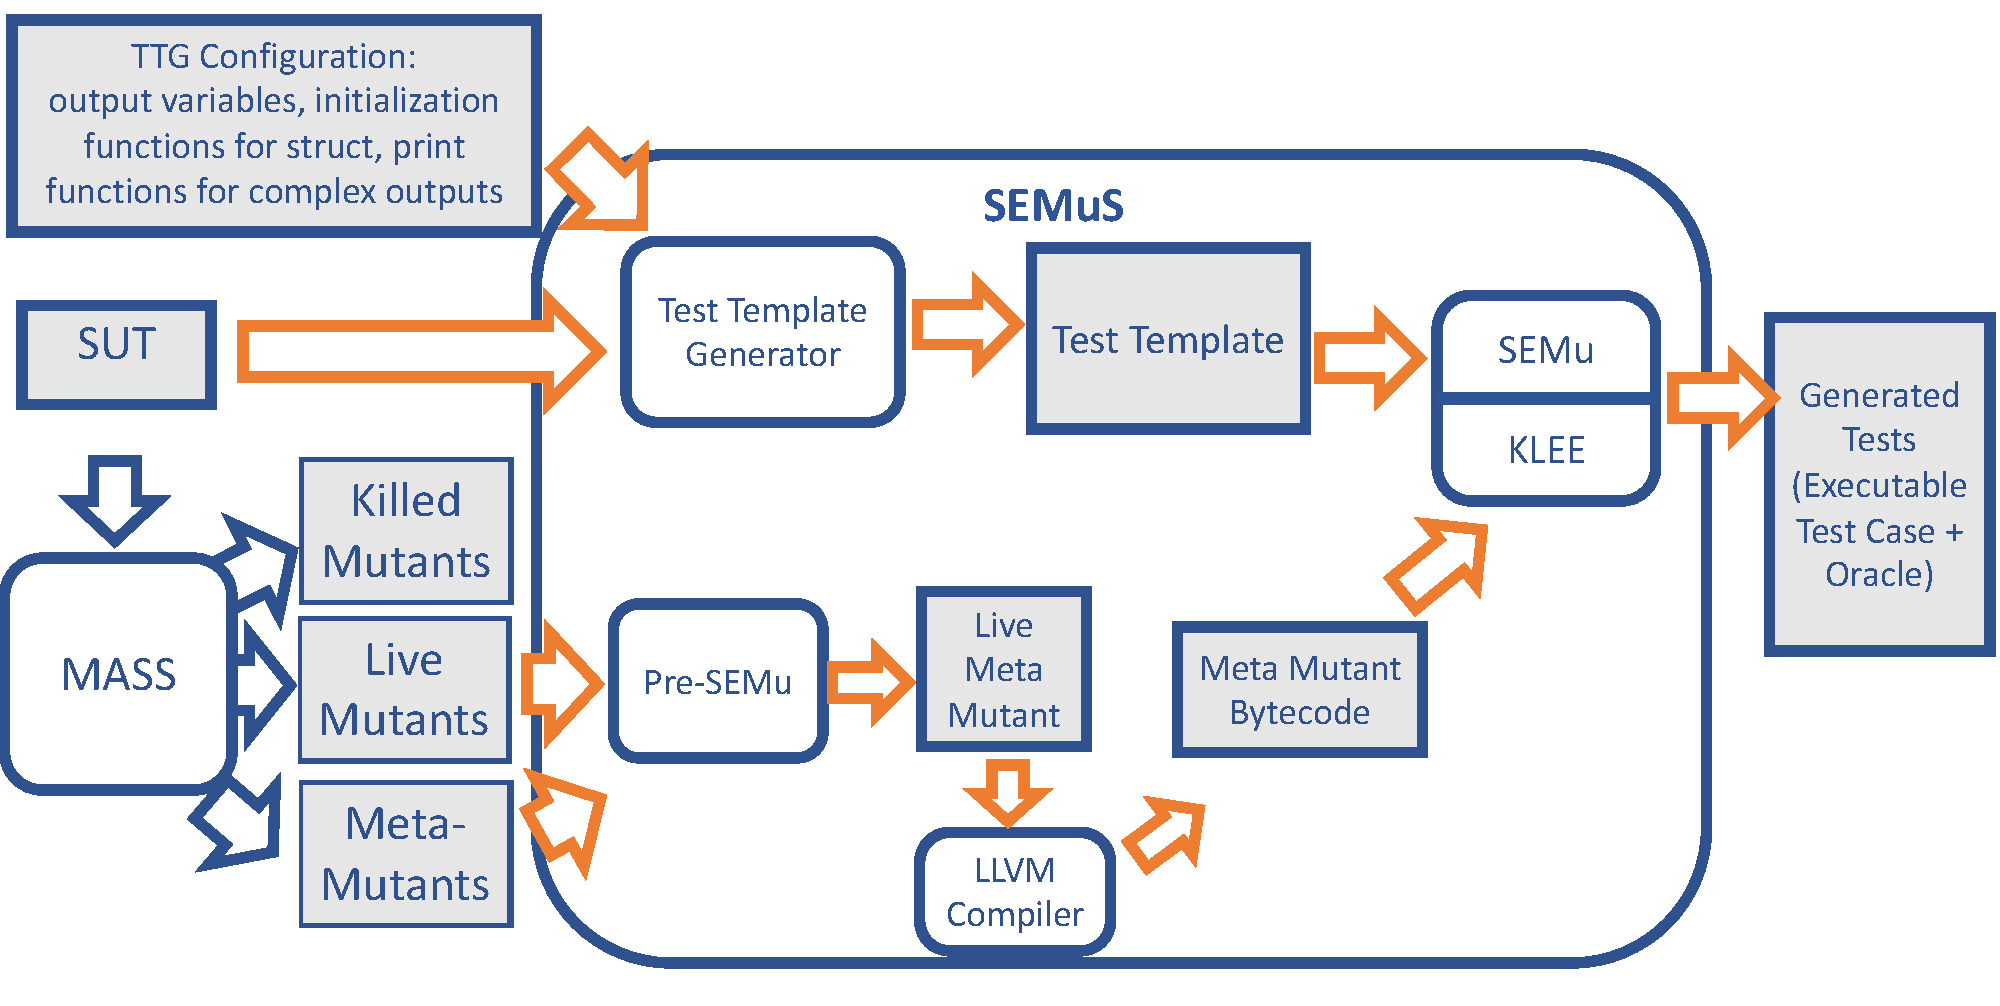
\includegraphics[width=0.8\textwidth]{images/semus-architecture2}
\caption{FAQAS-SEMuS Architecture and Workflow}
\label{fig:semus_architecture}
\end{center}
\end{figure}

%enable the adoption of SEMu in the space context. In particular, SEMuS (1) automates the generation of a test template including symbolic variables that guides the generation of test inputs, and (2) compiles the test template and the mutant into the format required by SEMu (i.e., LLVM-IR). 

\subsection{Test Template Generator}

The \INDEX{Test Template Generator} (TTG) component automates the generation of templates for the symbolic execution search. The component receives as inputs the SUT source code and the list of SUT functions. 

Listing~\ref{test_template} shows an example of a test template generated by the TTG. The TTG generates a template for every SUT function. The TTG parses the function arguments and declares them symbolic through use of the KLEE function \texttt{klee\_make\_symbolic}. Then, it adds a call to the function under analysis with symbolic values, and it saves the return value into a support variable (i.e., \texttt{result\_faqas\_semu} in Listing~\ref{test_template}). Finally, it generates a number of invocations of the \emph{printf} function that print the value of the software outputs and adds a return statement with the value returned by the function under test (e.g., \texttt{result\_faqas\_semu} in Listing~\ref{test_template}). 
Such \emph{printf} invocations are necessary because of the way SEMu determines that a mutant is killed; two are the cases in which the mutant is considered killed: (1) the main function returns a different return value, (2) different values are printed to the standard output. Consequently, it is necessary to print out all the values of the software outputs.
To select which variables to print, for every source file under test, the engineer can specify, in the SEMuS configuration file, the arguments (typically pointers) that should be either considered output or considered both input and outputs. By default, the TTG considers all the function arguments as inputs, in case some argument (e.g., a pointer to a memory buffer) is used both as input and as output the engineer shall specify it as such; similarly, in case some some argument (e.g., a pointer to a struct) is used to store outputs, the engineer shall indicate that it is an output. Moreover, since, in  the C language, the function \emph{printf} cannot automatically determine how to print the different fields specified in a data structure (i.e., it prints only the memory address of the pointer), the engineer can also specify how to printout the different fields of a data structure.

Listing~\ref{test_config} shows an example configuration file for SEMuS. In addition to output arguments (i.e., \emph{OUT\_\-ARGS\_NAMES}), input/output arguments (i.e., \emph{IN\_OUT\_ARGS\_NAMES}), and customized printf instructions (i.e., \emph{TYPES\_TO\_PRINTCODE}), the SEMuS configuration file enables the engineer to customize the generation of the test template further. Indeed, engineers can specify input argument types that should not be treated symbolically but that shall be initialized using a specific function of the SUT (i.e., \emph{TYPE\_TO\_INITIALIZATION\-CODE}); also, engineers can specify the fields, within such types (e.g., the attributes of a struct), that shall be treated symbolically.
Moreover, since the template returns the value of the function under test, the engineer can specify how to convert the returned value to int, if necessary (see parameter \emph{TYPES\_TO\_INTCONVERT}). Finally, in case the function under test receives a pointer to an array (which is typically passed as a pointer), the engineer can specify the size of such array (see parameter \emph{ARG\_TYPE\_TO\_ITS\_POINTER\_ELEM\_NUM}); by default, SEMuS assumes that a pointer refers to a single element (i.e., it is a pointer to a variable not an array).  


% !TEX root =  ../MAIN.tex

\begin{lstlisting}[style=CStyle, caption=SEMuS test template., label=test_template]
int main(int argc, char** argv) {
    // Declare variable to hold function returned value
    _Bool result_faqas_semu; 
    // Declare arguments and make input ones symbolic
    unsigned long pVal;
    int pErrCode;
    klee_make_symbolic(&pVal, sizeof(pVal), "pVal"); // Call function under test
    result_faqas_semu = T_INT_IsConstraintValid(&pVal, &pErrCode); // Make some output
    printf("FAQAS-SEMU-TEST_OUTPUT: %d\n", pErrCode);
    printf("FAQAS-SEMU-TEST_OUTPUT: %d\n", result_faqas_semu);
    return (int)result_faqas_semu;
}

\end{lstlisting}


\begin{lstlisting}[language={}, caption=Klee-test output, label=ktest]
ktest file : 'test000001.ktest'
args       : ['/MakeSym-TestGen-Input/direct/T_INT_IsConstraintValid/test.MetaMu.bc']
num objects: 2
object    0: name: b'model_version'
object    0: size: 4
object    0: data: b'\x01\x00\x00\x00'
object    1: name: b'pVal'
object    1: size: 8
object    1: data: b'\x00\x00\x00\x00\x00\x00\x00\x00'
\end{lstlisting}

% !TEX root =  ../MAIN.tex

\begin{lstlisting}[float=h, style=CStyle, caption=SEMuS configuration example., label=test_config]
{
"TYPES_TO_INTCONVERT": {},
"TYPES_TO_PRINTCODE": {"gs_timestamp_t": "printf(\"FAQAS-SEMU-TEST-OUTPUT: result_faqas_semu = tv_sec: %u, tv_nsec: %u\\n\", {}.tv_sec, {}.tv_nsec);"},
"OUT_ARGS_NAMES": ["pErrCode"],
"IN_OUT_ARGS_NAMES": ["base"],
"TYPE_TO_INITIALIZATIONCODE": {},
"TYPE_TO_SYMBOLIC_FIELDS_ACCESS": {},
"VOID_ARG_SUBSTITUTE_TYPE": "",
"ARG_TYPE_TO_ITS_POINTER_ELEM_NUM": {"char *": 6}
}
\end{lstlisting}


\subsection{Pre-SEMu}

The \INDEX{Pre-SEMu} component generates \INDEX{mutant schemata}; specifically, the component includes and compiles all the live mutants (i.e., MASS output) into a single bytecode file named the \emph{Meta Mutant}. SEMu will select which mutant to consider for test generation based on a parameter. The compilation of the Meta Mutant into LLVM bitcode is supported by the \emph{LLVM} compiler infrastructure. 

% !TEX root =  ../MAIN.tex



\begin{lstlisting}[style=CStyle, float=h, caption=Function T\_INT\_IsConstraintValid., label=original_meta]
flag T_INT_IsConstraintValid(const T_INT* pVal, int* pErrCode)
{
    flag ret = TRUE;
    (void)pVal;

    ret = ((*(pVal)) <= 50UL);
    *pErrCode = ret ? 0 :  ERR_T_INT;

    return ret;
}
\end{lstlisting}

\begin{lstlisting}[style=CStyle, float=h, caption=Mutant 1 of function T\_INT\_IsConstraintValid., label=meta_mutant_1]
flag T_INT_IsConstraintValid(const T_INT* pVal, int* pErrCode)
{
    flag ret = TRUE;
    (void)pVal;

    ret = ((*(pVal)) <= 50UL);
    *pErrCode = ret ? 1 :  ERR_T_INT;

    return ret;
}
\end{lstlisting}

\begin{lstlisting}[style=CStyle, float=h, caption=Mutant 2 of function T\_INT\_IsConstraintValid., label=meta_mutant_2]
flag T_INT_IsConstraintValid(const T_INT* pVal, int* pErrCode)
{
    flag ret = TRUE;
    (void)pVal;

    ret = ((*(pVal)) <= 50UL);
    *pErrCode = ret ? (-1) :  ERR_T_INT;

    return ret;
}
\end{lstlisting}

\begin{lstlisting}[style=CStyle, float=h, caption=Meta-Mutant for function T\_INT\_IsConstraintValid., label=meta_mutant_example]
flag T_INT_IsConstraintValid(const T_INT* pVal, int* pErrCode)
{
    flag ret = TRUE;
    (void)pVal;

    ret = ((*(pVal)) <= 50UL);

    klee_semu_GenMu_Mutant_ID_Selector_Func(1,2);
    *pErrCode = ret ? 
    	( klee_semu_GenMu_Mutant_ID_Selector==2 ?
    		((-1)):
		    (klee_semu_GenMu_Mutant_ID_Selector==1?
			    (1):
			    (0))) 
			    :  ERR_T_INT;
    klee_semu_GenMu_Post_Mutation_Point_Func(0,0);
    klee_semu_GenMu_Post_Mutation_Point_Func(1,2);

    return ret;
}
\end{lstlisting}

Listings~\ref{original_meta} provides the source code of function \emph{T\_INT\_IsConstraintValid}, while Listings~\ref{meta_mutant_1} and~\ref{meta_mutant_2} provide two example mutants generated by MASS.
Listing~\ref{meta_mutant_example} provides an example \INDEX{meta-mutant} including the same two mutants of Listings~\ref{meta_mutant_1} and~\ref{meta_mutant_2}. 
To select the mutants to analyze at runtime, SEMu relies on three support functions that shall be invoked within the eta-mutant:

\begin{itemize}
	\item \texttt{klee\_semu\_GenMu\_Mutant\_ID\_Selector\_Func}: function that takes two mutant IDs as arguments, representing a range of mutant IDs. It specifies where a portion of code containing mutants start.
    \item \texttt{klee\_semu\_GenMu\_Mutant\_ID\_Selector}: global variable that contains the ID of the mutant to be activated durng the analysis with SEMu.
	\item \texttt{klee\_semu\_GenMu\_Post\_Mutation\_Poin\_Func}: 
	function that takes two mutant IDs as arguments, it specifies where a portion of code containing mutants ends.
	It is used by SEMu to identify the portion of the code where to compare the state of the original and the mutated program and determine if the mutation has affected the program state (i.e., the \INDEX{necessity} condition to kill a mutant). In other words, it enables SEMu to perform conservative pruning and remove the mutant states that are not infected.
\end{itemize}

In Listing~\ref{meta_mutant_example}, mutant 2 from Listing~\ref{meta_mutant_2} appears on line 11 (indeed, the value \emph{-1} is selected when the mutant ID is equal to 2). Mutant 1 from Listing~\ref{meta_mutant_1} appears on line 12 (indeed, the value \emph{1} is selected when the mutant ID is equal to 1). The original software is represented by the mutant ID zero; indeed the value \emph{0} (i.e., what appears in line 7 of the Listing~\ref{original_meta}) is selected on line 14 (i.e., when the mutant ID is neither \emph{2} nor \emph{1}).

\subsection{KLEE-SEMu}



\INDEX{KLEE-SEMu} is the underlying test generation component, previously described in Section~\ref{sec:testGen:CP}. This component receives as inputs the \emph{LLVM bitcode} of the \emph{Meta Mutant} and the \emph{Test Template} for the function under test, and proceeds to apply dynamic symbolic execution to generate test inputs to kill the mutants. The output of this component are the \emph{KLEE tests}.

% \TODO{you need to list what are "the parameters of the execution"}
A \INDEX{KLEE test} is a binary file that contains information about the execution of KLEE such as the entry point of the analysis, and the generated test inputs.


An example of a KLEE test is presented in Listing~\ref{ktest}. The field \emph{args} report the entry point of the analysis; in this case, the test generation was performed for live mutants present in the function \texttt{T\_INT\_Is\-Constraint\-Valid}, which SEMuS stores in a dedicated folder. The fields named \emph{object} provide information about the outputs generated by KLEE (e.g., the generated test inputs). 
For each object, the KLEE test provides a \emph{name} (usually the name of the symbolic variable), its \emph{size}, and the actual \emph{value} generated by KLEE through constraint solving (usually this is reported in binary form).
Objects are numbered. Object number \emph{0} reports information about the data structure used by KLEE, that is, the version of the structure. The other objects report information about the generated test inputs.
Our example shows that one value of size 8 was generated for the variable \texttt{pVal}, the data field shows the binary representation of the \texttt{pVal} variable, in this case \texttt{pVal=0}.

% !TEX root =  ../MAIN.tex
\begin{lstlisting}[float=t, language={}, caption=Klee-test output, label=ktest]
ktest file : 'test000001.ktest'
args       : ['/MakeSym-TestGen-Input/direct/T_INT_IsConstraintValid/test.MetaMu.bc']
num objects: 2
object    0: name: b'model_version'
object    0: size: 4
object    0: data: b'\x01\x00\x00\x00'
object    1: name: b'pVal'
object    1: size: 8
object    1: data: b'\x00\x00\x00\x00\x00\x00\x00\x00'
\end{lstlisting}

\subsection{KTest to Unit Test}

% !TEX root =  ../MAIN.tex

\begin{lstlisting}[float=t, style=CStyle,  caption=Generated test case, label=gen_test_case]
#include <stdio.h>
#include <string.h>

#include "asn1crt.c"
#include "asn1crt_encoding.c"
#include "asn1crt_encoding_uper.c"


int main(int argc, char** argv)
{
    (void)argc;
    (void)argv;

    // Declare variable to hold function returned value
    _Bool result_faqas_semu;

    // Declare arguments and make input ones symbolic
    unsigned long pVal;
    int pErrCode;
    memset(&pVal, 0, sizeof(pVal));
    const unsigned char pVal_faqas_semu_test_data[] = {0x00, 0x00, 0x00, 0x00, 0x00, 0x00, 0x00, 0x00};
    memcpy(&pVal, pVal_faqas_semu_test_data, sizeof(pVal)); // Unsigned val is 0

    // Call function under test
    result_faqas_semu = T_INT_IsConstraintValid(&pVal, &pErrCode);

    // Make some output
    printf("FAQAS-SEMU-TEST_OUTPUT: pErrCode = %d\n", pErrCode);
    printf("FAQAS-SEMU-TEST_OUTPUT: result_faqas_semu = %d\n", result_faqas_semu);
    return (int)result_faqas_semu;
}
\end{lstlisting}



The component \INDEX{KTest to Unit Test} (KTU) converts a KLEE test into a human readable, compilable, and executable C test case. The unit test case generated by KTU, match the test template generated by TTG except for the declaration of variables where symbolic variables are replaced with concrete variables initialized with the values stored in the KTest file.
 
Listing~\ref{gen_test_case} shows an example of a test case generated for a mutant present in the function \texttt{T\_INT\_Is\-ConstraintValid}. For instance, line 20 shows that the variable \texttt{pVal} is initially filled with zeros, then in line 21, it is filled with the value stored in the variable \texttt{pVal\_faqas\_semu\_test\_data}, which holds the binary output produced by KLEE. In line 25, the function under test is invoked with the concrete value of \texttt{pVal}. 

The test case generated by the KTU prints the function return value and the value of every variable passed by reference, using the same instructions of the test template.
KTU cannot generate test assertions because only engineers can know, based on specifications, what are the values to be expected at the end of the test case execution.
However, the generated printf invocations still play the role of an oracle for regression testing, as explained in the next sections.

\subsection{Test suite augmentation} 
\label{sec:Semus:augment}
The procedure for testing with SEMuS is shown in Figure~\ref{fig:semus:test:example}.
In Step 1, the engineer executes SEMuS, which generates an output folder for every live mutant that is killed by the generated test cases.
Every folder contains: a script (i.e., \emph{runTest.sh}) that can be used to execute the generated test case, (2) the test case itself (i.e., test1.c), and (3) a text file with extension \emph{.expected} that contains the output that is observed when executing the test case with the SUT.
In Step 2, the engineer visually inspects every file with extension \emph{.expected} to determine if the observed output matches the specifications; if not, the software is faulty and needs to be fixed. In this case mutation testing enables detecting a fault. 
After verifying all the generated files with extension \emph{.expected} the engineer can reuse the test cases generated by SEMuS for regression testing in future versions of the SUT. Basically, the output folders generated by SEMuS become part of the test suite of the SUT.

When there is a new version of the SUT (Step 3, in Figure~\ref{fig:semus:test:example}), the folder with the source code of the SUT is replaced with the new version of the SUT (this can be done automatically with version control software).
The engineer can then trigger test execution by simply re-executing all the scripts \emph{runTest.sh} generated by SEMuS.
The script \emph{runTest.sh} first executes the test case (Step 4.1), then it stores the test outputs into a text file with extension \emph{.got}, finally if compares the observed output with the output generated for the previous version. If the function under test was not modified, differences may indicate that the test case FAILED.

\begin{figure}[h]
\begin{center}
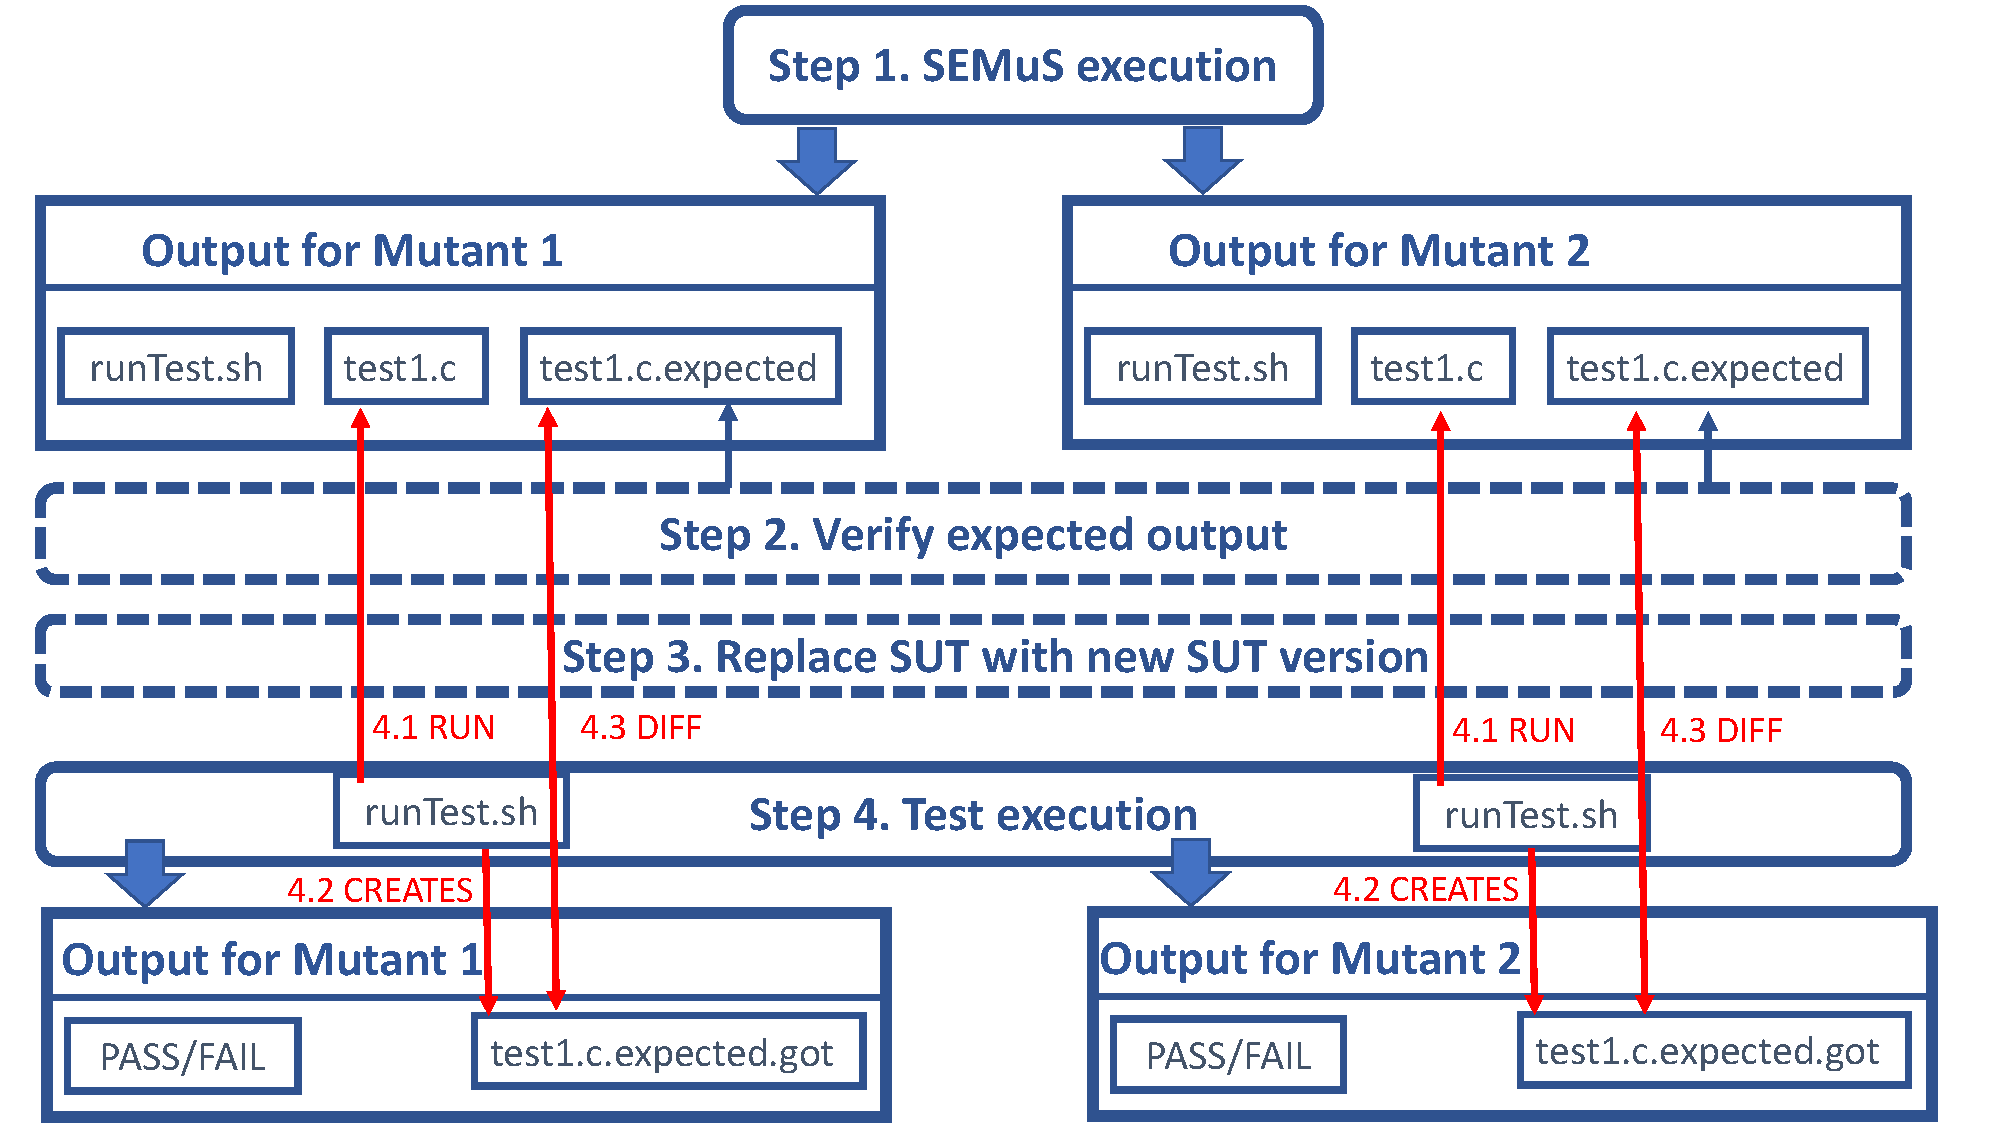
\includegraphics[width=0.8\textwidth]{images/semus-out}
\caption{Workflow for test suite augmentation with SEMuS}
\label{fig:semus:test:example}
\end{center}
\end{figure}

\subsection{Live mutants}

SEMuS may not be capable of selecting test inputs that kill the mutant under analysis. We may distinguish two cases:
\begin{itemize}
\item SEMuS execution terminates and no test case is generated.
\item SEMuS execution does terminate (i.e., it is killed after a timeout configured by the end-user, usually 15 minutes are sufficient to generate test cases).
\end{itemize}

In the first case, SEMuS has successfully exercised all the execution paths covering the mutated statements but did not identify inputs that satisfy the killing conditions. This may case indicate that the mutant is equivalent and may be discarded (however, the engineer shall verify that the test template is configured correctly). Also, we may be in such situations when some of the functions under test belong to libraries not compiled with LLVM that, consequently are not correctly processed by KLEE-SEMu; to detect these cases the engineer shall look for errors in the output generated by KLEE.

In the second case, SEMuS did not complete the analysis of the possible execution paths covering the mutated statement. Such cases may indicate that test generation is complex and probably an engineer may more efficiently select test inputs than the underlying constraint solving solution implemented by KLEE-SEMu.

% !TEX root =  ../MAIN.tex
\clearpage
\section{Data-driven Mutation Analysis: DAMAt}

\renewcommand{\APPR}{DAMAt\xspace{} }


\subsection{Overview}

In this Section, we propose \INDEX{data-driven mutation analysis}, 
a new mutation analysis paradigm
that alters the data exchanged by software components to evaluate the capability of a test suite to detect interoperability faults. Also, we present a technique, \INDEX{data-driven mutation analysis with tables} (\APPR),
to automate data-driven mutation analysis by relying on
a fault model that captures, for a specific set of components, both the characteristics of the data to mutate (e.g., the size and structure of the messages generated by the ADCS) and the types of fault that may affect such data (e.g., a  value out of the nominal range). The latter is formalized as a set of parameterizable mutation operators. 
To simplify adoption, we rely on fault models in tabular form where each row specifies, for a given data item, what mutation operator (along with its corresponding parameter values) to apply to which elements of the data item.
At runtime, \APPR modifies the data exchanged by components according to the provided fault model (e.g., replaces a nominal voltage value with a value out of the nominal range).






\INDEX{Data-driven mutation analysis} aims to evaluate the effectiveness of a test suite in detecting \INDEX{semantic interoperability \UPDATED{faults}}. 
It is achieved by modifying (i.e., mutating) the data exchanged by CPS components. It generates \INDEX{mutated data} that is representative of data that might be observed at runtime in the presence of a component that behaves differently than expected in the test case; also, it mutates  data that is not automatically corrected by the software 
(e.g., through cyclic redundancy check codes)
%(e.g., through CRC mechanisms, which aim to correct technical interoperability problems) 
and thus causes software failures (i.e., the mutated data shall have a different semantic than the original data). For these reasons, data mutation is driven by a fault model specified by the engineers based on domain knowledge.

Although different types of fault models might be envisioned,
%see background
we propose a technique (\INDEX{data-driven mutation analysis with tables}, \APPR),
which automates data-driven mutation analysis by relying on
a tabular \CHANGED{block model}, itself tailored to the \UPDATED{SUT} through predefined mutation operators.
To concretely perform data mutation at runtime, \APPR relies on a set of \INDEX{mutation probes} that shall be integrated by software engineers into the software layer that handles the communication between components. The runtime behaviour of mutation probes (i.e, what data shall be mutated and how) is driven by the fault model. Thus, \APPR can automatically generate the implementation of mutation probes from the provided fault model.
Depending on the CPS, probes might be inserted either into the \UPDATED{SUT}, into the simulator infrastructure, or both.
For example, Figure~\ref{fig:appr:mutateProbesInserted} shows the architecture of the \ESAIL satellite system with mutation probes integrated into the SVF
%\footnote{Software Validation Facility~\cite{Isasi2019}; it usually includes one or more simulators, an emulator to run the code compiled for the target hardware, and test harnesses.} 
functions that handle communication with external components (PDHU, GPS, and ADCS in this case). 






\APPR works in six steps, which are shown in Figure~\ref{fig:appr:approach}. 
In Step 1, based on the provided methodology and predefined mutation operators, the engineer prepares a fault model specification tailored to the SUT.
% capturing the data format and the types of faults that shall be injected for every data item exchanged by the system components.
In Step 2, \APPR generates a mutation API with the functions that modify the data according to the provided fault model.
In Step 3, the engineer modifies the \UPDATED{SUT} by introducing mutation probes (i.e., invocations to the mutation API) into it.
\REVTOOL{P-2}{Instead of modifying the SUT the engineer may modify the test harness (e.g., the SVF simulator); such choice depends on the software under test, if the test cases are executed through a simulator, such choice prevents introducing damaging changes into the SUT (e.g., delay task execution and break strict real-time requirements).}
In Step 4, \APPR generates and compiles mutants. 
Since the \APPR mutation operators may generate mutated data by applying multiple mutation procedures, \APPR may generate several mutants, one for each \UPDATED{mutation operation (i.e., a mutation procedure configured for a data item, according to our terminology, see Section~\ref{sec:mutantsGeneration})}.
In Step 5, \APPR executes the test suite with all the mutants including a mutant (i.e., the coverage mutant) which does not  modify the data but traces the coverage of the fault model.
In Step 6, \APPR generates mutation analysis results.

%\UPDATED{
%In our context, the \emph{software under test (SUT)} is the CPS embedded software that is verified by a test suite, which is the target of data-driven mutation analysis. Therefore, we refer to the software developed by the engineers as the \emph{original SUT}. An \emph{SUT mutant} (simply, a \emph{mutant}) is a version of the SUT that integrates a \emph{mutation probe} and shall make test cases fail. 
%%A mutation operator simulates one specific interoperability error (a specific type of that automatically alters data by applying one specific \emph{mutation operation}.
%}

In the following sections we describe the structure of our fault model and each step of \APPR.

\begin{figure}[h]
	\centering
		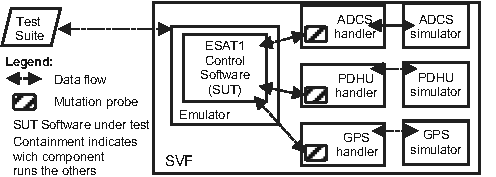
\includegraphics[width=8.4cm]{damat/images/dataMutationExample}
		\caption{\CHANGED{Data mutation probes integrated into \ESAIL.}}
		\label{fig:appr:mutateProbesInserted}
	\end{figure}

\begin{figure}[h]
	\centering
		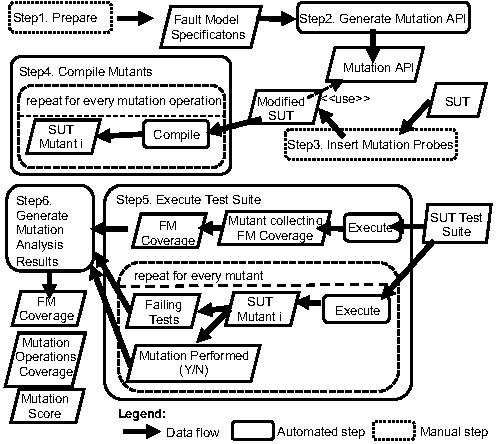
\includegraphics[width=8cm]{damat/images/dataDrivenBufferProcess}
		\caption{The \APPR process.}
		\label{fig:appr:approach}
	\end{figure}


\subsubsection{Fault Model Structure}
\label{sec:faultModelStructure}





The \APPR fault model enables the specification of the format of the data exchanged between components along with the type of faults that may affect such data. 
In this paper, we refer to the data exchanged by two components as \INDEX{message}; also, each CPS component may generate or receive different \INDEX{message types}.
For a single CPS, more than one fault model can be specified. For example, in the case of \ESAIL{} we have defined one fault model for every message type that could be exchanged by the three components under test (i.e., ADCS, PDHU, and GPS). In total, for \ESAIL, we have 14 fault models, 10 for the communication concerning ADCS (we have 10 different message types), 3 for PDHU, and 1 for GPS.

The \APPR fault model enables the modelling of data that is exchanged through a specific data structure: the data buffer. This was decided because it is a simple and widely adopted data structure for data exchanges between components in CPS. Also, more complex data structures (e.g., hierarchical ones like trees) are often flattened into data buffers in order to be exchanged by different components (e.g., through the network). When the CPS software is implemented in C or C++ (common CPS development languages) data buffers are implemented as arrays. Figure~\ref{fig:appr:bufferStructure} shows three block diagrams representing (part of) the buffer structure used to exchange messages of type InterfaceHouseKeeping and InterfaceStatus in \ESAIL.

A data buffer is characterized by a \INDEX{unit size} that specifies the dimension, in bytes, of the single cell of the underlying array and a \INDEX{buffer size}, which specifies the total number of units belonging to the buffer. Each data buffer can contain one or more \INDEX{data items}; the size of data items may vary as they may span over multiple units. Also, each data item is interpreted by the CPS software according to a specific \INDEX{representation} (e.g., integer, double, etc.). 
In \ESAIL, the unit size is one byte and the data items may span over one or two buffer units (see Figure~\ref{fig:appr:bufferStructure}). 
%Figure~\ref{} provides an example buffer instance for a \emph{Magnetorquer Set PWM RSP message}.

The \APPR fault model enables engineers to specify (1) the \emph{position} of each data item in the buffer, (2) their \emph{span}, and (3) their \emph{representation type}. Our current implementation supports six data representation types: int, long int, float, double, bin (i.e., data that should be treated in its binary form), hex (i.e., data that should be treated as hexadecimal).
Further, for each data item, \APPR enables engineers to specify one or more data faults using the mutation operator identifiers. For each operator, the engineer 
shall provide values for the required configuration parameters.

Table~\ref{table:operators} provides the list of mutation operators included in \APPR along with their description. The \APPR mutation operators generate \INDEX{mutated data item instances} through one or more \INDEX{mutation procedures}, which are the functions that generate a mutated data item instance given a correct data item instance observed at runtime. For example, the \emph{VAT} operator includes only one mutation procedure (i.e., setting the current value above the threshold) while the \emph{VOR} operator includes two mutation procedures, which are
(1) replacing the current value with a value above the specified valid range and (2) replacing the current value with a value below the valid range.
The operators VOR, BF, INV, and SS have been inspired by related work~\cite{di2015generating,PeachFuzzer,Matinnejad19}; the operators VAT, VBT, FVAT, FVBT, FVOR, IV, ASA,  and HV
are a contribution of this paper and were derived and conceptualised as a result of discussion with domain experts.
Although other data representation types (e.g., null terminated strings) and operators (e.g., replacement of a random char in a string) might be envisioned, in this paper, we focus on operators that are necessary in the CPS context, based on our experience.
For example, CPS components are unlikely to exchange strings.
%are a contribution of this paper, based on discussion with domain experts. 

\begin{figure}
	\centering
		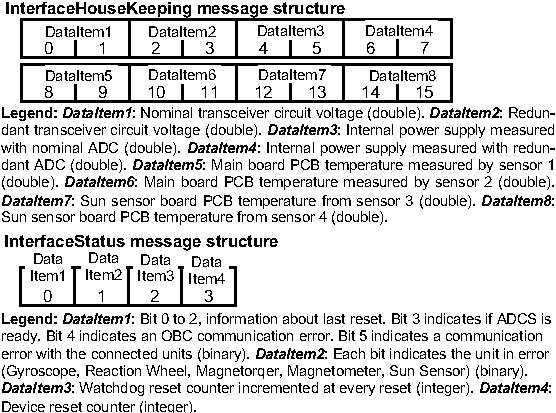
\includegraphics[width=8.4cm]{damat/images/BufferStructuresSmall}
		\caption{Structure of data buffers in \ESAIL.}
		\label{fig:appr:bufferStructure}
	\end{figure}
	
	% !TEX root = ../MAIN-DataDrivenMutationAnalysis.tex


\begin{table*}[tb]
\caption{Data-driven mutation operators}
\label{table:operators}
\scriptsize
\begin{tabular}{|p{40mm}|p{90mm}|}
\hline
\textbf{Fault Class}&\textbf{Description}\\
\hline
Value above threshold (VAT)&
Replaces the current value with a value above the threshold T for a delta (\D). 
\\
\hline
Value below threshold (VBT)&
Replaces the current value with a value below the threshold T for a delta (\D). 
\\
\hline
Value out of range (VOR)&
Replaces the current value with a value out of the range $[MIN;MAX]$.\\
\hline
Bit flip (BF)&
A number of bits randomly chosen in the positions between MIN and MAX are flipped.
\\
\hline
Invalid numeric value (INV)&
Replace the current value with a mutated value that is legal (i.e., in the specified range) but different than current value. 
\\
\hline
Illegal Value (IV)
&
Replace the current value with a value that is equal to the parameter \emph{VALUE}. 
\\
\hline
Anomalous Signal Amplitude (ASA)
&
The mutated value is derived by amplifying the observed value by a factor \emph{V} and by adding/removing a constant value \D from it. 
\\
\hline
Signal Shift (SS)
&
The mutated value is derived by adding a value \D to the observed value. 
\\
\hline
Hold Value (HV)
&
This operator keeps repeating an observed value for $V$ times. It emulates a constant signal replacing a signal supposed to vary.
\\
\hline
Fix value above threshold (FVAT)&
In the presence of a value above the threshold, it replaces the current value with a value below the threshold T for a delta \D. 
\\
\hline
Fix value below threshold (FVBT)&
It is the counterpart of FVAT for the operator VBT.
\\
\hline
Fix value out of range (FVOR)&
In the presence of a value out of the range  $[MIN;MAX]$ it replaces the current value with a random value within the range. 
\\
\hline
\end{tabular}
\end{table*}%

\clearpage

%\begin{figure}
%	\centering
%		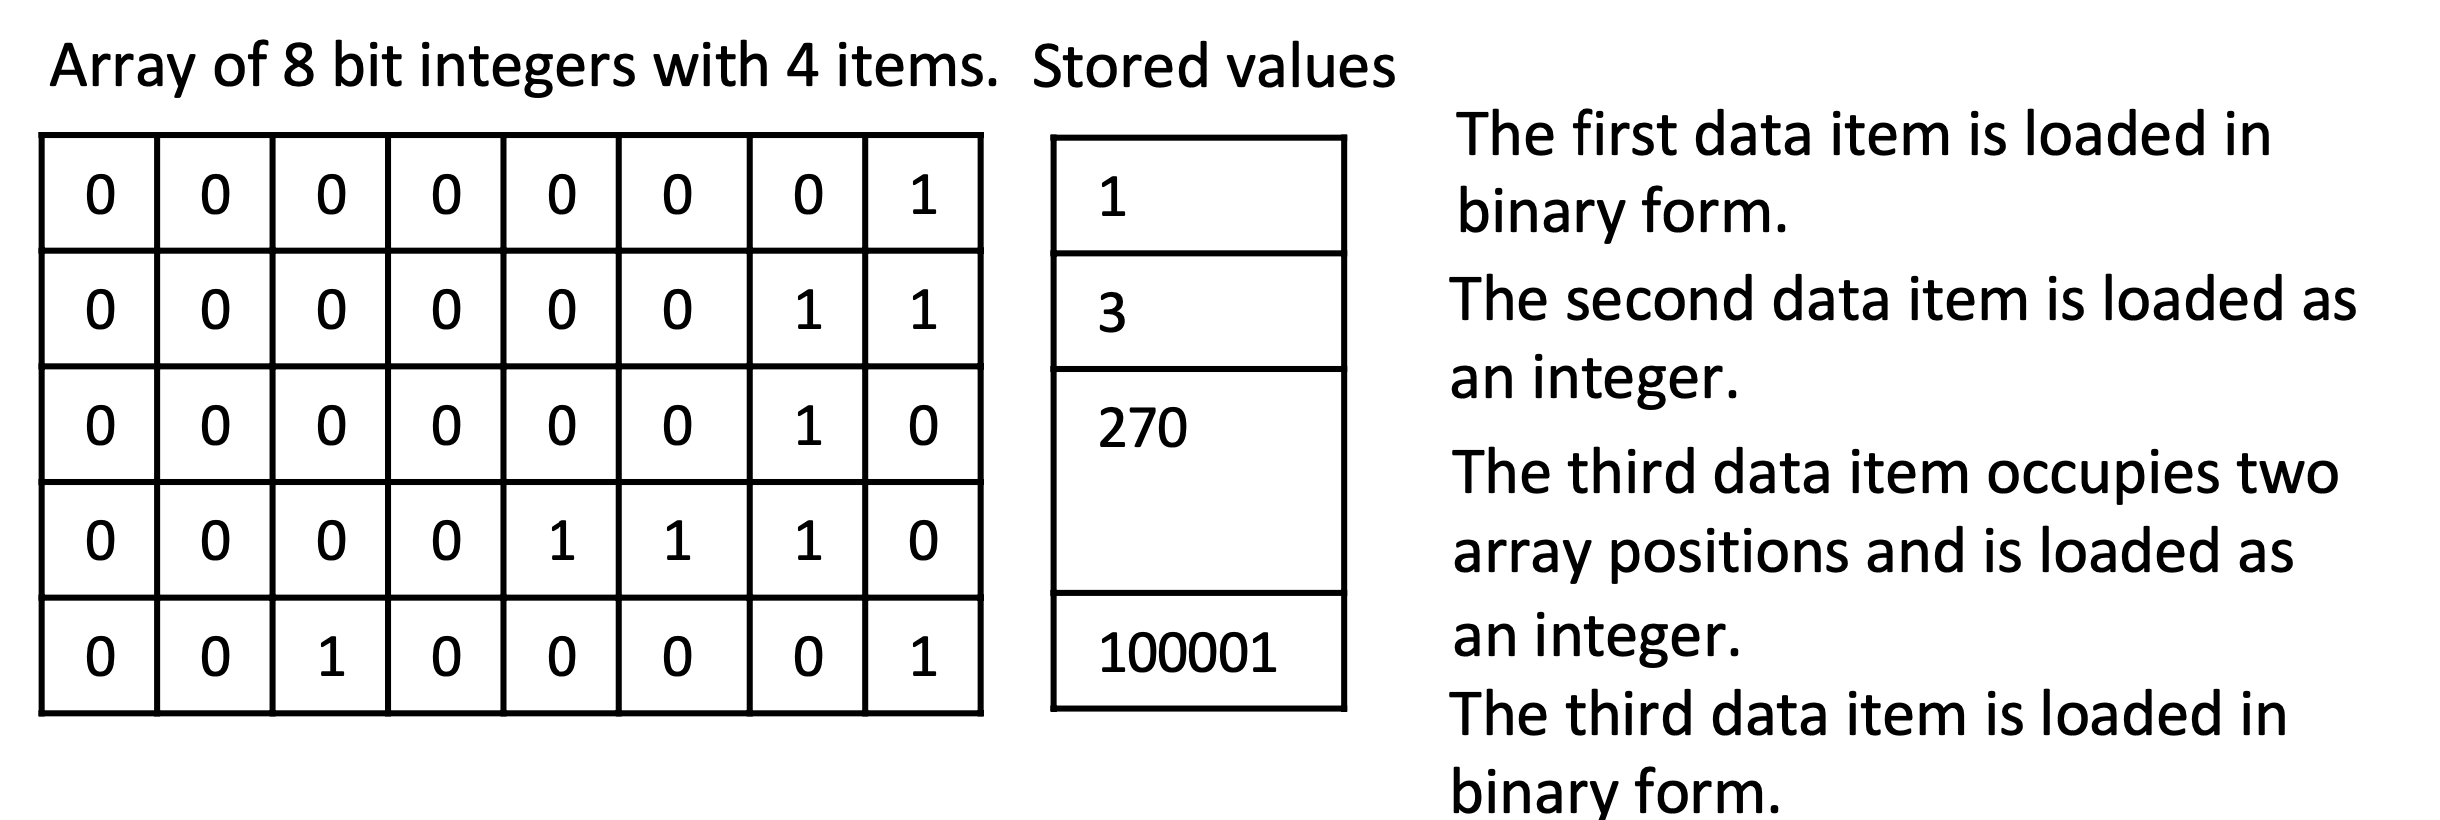
\includegraphics[width=8cm]{damat/images/bufferExample}
%		\caption{Example of a data buffer. \TODO{UPDATE PICTURE}}
%		\label{fig:appr:buffer}
%	\end{figure}

\subsubsection{Fault Modelling Methodology (Step 1)}
\label{sec:methodology}

% !TEX root =  ../MAIN-DataDrivenMutationAnalysis.tex

%
%\setlength\LTleft{0pt}
%\setlength\LTright{0pt}
%\begin{longtable}{@{\extracolsep{\fill}}|p{2.5cm}|p{5cm}|p{5cm}|@{}}
%\toprule


\begin{table}[tb]
\caption{\APPR fault modelling methodology}
\label{table:method}
\center
\scriptsize
\begin{tabular}{|
@{\hspace{1pt}}>{\raggedleft\arraybackslash}p{10mm}@{\hspace{1pt}}|
@{\hspace{1pt}}>{\raggedleft\arraybackslash}p{15mm}@{\hspace{1pt}}|
@{\hspace{1pt}}>{\raggedleft\arraybackslash}p{15mm}@{\hspace{1pt}}|
@{\hspace{1pt}}>{\raggedleft\arraybackslash}p{10mm}@{\hspace{1pt}}|
@{\hspace{1pt}}>{\raggedleft\arraybackslash}p{13mm}@{\hspace{1pt}}|
@{\hspace{1pt}}>{\raggedleft\arraybackslash}p{17mm}@{\hspace{1pt}}|
}
\hline
\textbf{Data} \textbf{nature}&\textbf{Representation} \textbf{type}&\textbf{Dependencies}&\textbf{\# of input} \textbf{partitions}&\textbf{Operators}&\textbf{Comments}\\
\hline
numerical&I, L, F, D&stateless/stateful&2&[VAT,FVAT]&Nominal below T\\
&&&&or [VBT,FVBT]&Nominal above T\\
\cline{4-6}
&&&3 or more&[VOR,FVOR]&\\
\cline{3-6}
&&stateful&&INV&For valid range\\
\cline{4-6}
&& &&[VOR,FVOR]&For out of range\\
\cline{3-6}
&&signal&&ASA, SS, HV&\\
\hline
categorical&I, H&N/A&N/A&IV&\\
\cline{2-6}
%&string&N/A&N/A&BF\\
%\cline{2-5}
&B&N/A&N/A&BF&\\
\hline
ordinal&I, H&N/A&N/A&ASA&\\
\hline
other&B&N/A&N/A&BF&\\
\hline
\end{tabular}\\
\textbf{Legend:} N/A not applicable.
\end{table}
%\normalsize

The fault model shall enable the specification of 
all possible interoperability problems in the SUT while minimizing equivalent and redundant mutants.
Equivalent mutants have the same observable output as the original SUT. 
Instead, redundant mutants have the same observable output as other mutants.
We use the term \INDEX{observable output} to refer to any output that can be verified by the test suite.
The equivalent or redundant nature of a mutant depends
on the equivalence relation for observable outputs
(i.e., how to determine if two outputs are the same).
In a testing context, such equivalence relation depends on the type of testing being performed. For example, system test cases, different than unit test cases,  are unlikely to verify the values of all the state variables of the system and thus mutants that are nonequivalent for unit test suites might be considered equivalent for system test suites. 
For example, in satellite systems, the correctness of the GPS triangulation algorithm output is verified by unit test cases; system test cases, instead, verify 
if the software takes appropriate actions when the satellite is out of orbit. Consequently, slight changes in the coordinates communicated by the GPS component may not lead to any change in the observable output verified by the test suite.
%When defining a fault model, engineers shall thus select and configure mutation operators in such a way that the mutations performed trigger changes in the observable output of the SUT (to avoid equivalent mutants) and (2) distinct mutations do not lead to the same observable outputs (to avoid redundant mutants).


We provide a set of guidelines for the definition of fault models that 
are summarized in Table~\ref{table:method}. 
For guidance,
% are based on the characteristics of the data being exchanged by CPS components.
we account for the nature of the data (i.e., numerical, categorical, ordinal, or binary) and their representation type.
Also, for numerical data, 
we consider 
%the type of measurement, that is, if the data is counted (i.e., it is discrete) or measured (i.e., it is continuous) and
%For numerical data, mutations shall be defined taking into consideration
the data dependencies, that is how data values depend on the previously observed values; we identified three categories: stateless (i.e., there are no dependencies between consecutive values), stateful (i.e, values depend on previous ones), and signal (i.e., values derive from a function of independent variables like time).
\CHANGED{Data dependencies determine the granularity of the mutation (i.e., with data dependencies, small differences shall be noticed); for non numerical data, we do not provide mutation operators with different granularities and data dependencies can be ignored.}
%on previous values and the time in which they are observed).

 

For \INDEX{stateless numerical data}, our guidelines are driven by input space partitioning concepts~\cite{Ammann:Offutt:2008}.
Indeed, given equivalence relations among outputs, it is unlikely that every change in \INDEX{stateless numerical data} will result into nonequivalent mutants; however, we can partition the input domain into regions with equivalent values (partitions).
Precisely, we rely on the  
\INDEX{interface-based input domain modeling} approach~\cite{Ammann:Offutt:2008}:
%Within data-driven mutation analysis, 
for each data item we identify a number of input partitions (set of values or value ranges) according to the interface specifications of the interacting components.
%each data item represents an input partition that shall be split into sets of values (or value ranges) identified according to the interface specifications of the interacting components.
%an input partition corresponds to a single data item and it shall be split into a set of blocks defined according to the interface specifications of the interacting components. 
In our methodology, the number and type of mutation operators selected for stateless numerical data depend on the number of input partitions identified.
With \emph{two input partitions} (e.g., nominal and exceptional data values), engineers can rely either on the pair [VBT,FVBT] or the pair [VAT,FVAT]. 
%Engineers shall select the pair of operators that simplifies the reading of the fault model.
%FABRIZIO: initially, I have explained what I mean with simplyfiy the reading (see below), however, these are details that may not be that necessary in a 10 pages conference paper.
%Engineers shall select the pair of operators that simplifies the reading of the data model; precisely, when the two input partitions capture  ranges for nominal and exceptional data values, the selection depends on how exceptional cases are identified (i.e., below or above the threshold). For other cases (i.e., two input partitions not related to exceptional cases), engineers can select any of the two pairs.
With \emph{three partitions}, engineers must configure one VOR and one FVOR operator. If a different delta (\D) is considered for the upper and lower bounds, engineers may configure two pairs [VBT,FVBT] and [VAT,FVAT], for the lower and upper bound, respectively. In the presence of \emph{more than three} partitions, engineers shall configure one [VOR,FVOR] pair for each extra partition above three (e.g., two pairs in the case of five partitions). The parameter \D{} is used to determine the partition to which the mutated data belongs. 
%Please note that mutants belonging to each pair shall not lead to redundant mutants.
%Engineers can configure multiple [VOR,FVOR] pairs in case several combinations needs to be tested.


In the presence of \INDEX{stateful data}, replacement with random values in the valid range (i.e., the INV operator) will lead to nonequivalent mutants (e.g., because it leads to data values that are systematically different than the values expected for the current system state). Alternatively, the valid data range might be partitioned as for stateless data. However, to avoid redundant mutants, engineers should rely either on the INV operator or the partitioning of the valid data range. 
The effect of data outside the valid data range should instead be verified by means of the [VOR, FVOR] pair.

For \INDEX{signal values}, depending on the shape of the expected signal, engineers should configure one operator among the ASA, SS, and HV. The configuration of more than one of these operators may lead to redundant mutants (e.g., because each of them triggers the same warning in the SUT).

With \INDEX{categorical data} represented using \emph{integers and hexadecimals}, engineers must configure one IV operator for each possible value; indeed, a change in the observed category shall trigger a different behaviour in the SUT. 
%With categorical data represented using labels (e.g., strings), engineers shall configure one BF operator with the MAX parameter set to the minimum number of characters taken by the string; indeed, such a bit flip mutation ensures to alter the transmitted label (e.g., change a characater of the string label) and thus introduce a nonequivalent mutant.
With categorical data in \emph{binary form}, each bit indicates a specific class (e.g., the unit in error for the DataItem2 in the IFStatus message of Figure~\ref{fig:appr:bufferStructure}).  
To verify that the test suite can detect any possible category change, engineers must configure two BF operators for every bit (both MIN and MAX must coincide with the bit position), one operator must flip a bit when it is set (i.e., $\mathit{STATE}=1$), and the last one when it is unset (i.e., $\mathit{STATE}=0$). 
%If only two categories are represented by the data item (i.e., only one bit is used), it is sufficient to configure one BF operator.

For \INDEX{ordinal data}, which is represented by means of either integers or hexadecimals, we suggest to apply the ASA operator with \emph{T} being set to the middle point of the ordinal scale and \D set to the step distance between consecutive data (usually $1$). For data in binary form (e.g., pictures), engineers must configure a BF operator to flip a number of bits  that is sufficient to alter the semantics of the data (e.g., introduce sufficient noise in images).

%, and values are selected from each region.
%
%==> the structure of the input domain in terms of input characteristics. The test engineer creates a partition for each characteristic. The partition is a set of blocks, each of which contains a set of values. From the perspective of that particular characteristic, the values in each block are considered equivalent.



%observable output difference.
%For stateless data, changes in the observable output of the SUT shall be expected when a data item value is replaced with a data item value that belongs to a differ
%
%For visible output we refer to any (e.g., two mutants causing the same failures in the test suite).
%
%We have an equivalent mutant..
%In system and integration test suites (i.e., the ones exercising components interoperability) it is unlikely that any change in the data exchanged by components result in a test case failure. 
% 
%
%Somehow, to make a system test case fail, the granularity of the error observed the data shall be coarser than the one require to make a unit test case fail. In a mutation analysis context this means that, to avoid equivalent mutants (that is 
%
%targeting functional correctness of the results computed after processing
%
%and thus make test cases fail.

% !TEX root = ../MAIN.tex
\begin{table}[h]
\begin{center}
\scriptsize
\begin{tabular}{|p{2cm}|p{2cm}|p{4cm}|p{6cm}|}
\hline
\textbf{Fault Class}&\textbf{Types}&\textbf{Parameters}&\textbf{Description}\\
\hline
Value above threshold (VAT)&
\begin{minipage}{6cm}
INT\\
LONG INT\\
FLOAT\\
DOUBLE
\end{minipage}
&
\begin{minipage}{6cm}
T: threshold\\
D: delta with respect to threshold\\
\end{minipage}
&
\begin{minipage}{6cm}
The value is above a threshold T for a delta D. 

\EMPH{Data mutation operation:} The mutation is performed by replacing the current value (a number) with a value of the same type that is equal to $(T+D)$.
\end{minipage}
\\

\hline
Value below threshold (VBT)&
\begin{minipage}{6cm}
INT\\
LONG INT\\
FLOAT\\
DOUBLE
\end{minipage}
&
\begin{minipage}{6cm}
T: threshold\\
D: delta with respect to threshold\\
\end{minipage}
&
\begin{minipage}{6cm}
The value is below a threshold T for a delta D. 

\EMPH{Data mutation operation:} The mutation is performed by replacing the current value (a number) with a value of the same type that is equal to $(T-D)$.
\end{minipage}
\\



\hline
Value out of range (VOR)&
\begin{minipage}{4cm}
INT\\
LONG INT\\
FLOAT\\
DOUBLE
\end{minipage}
&
\begin{minipage}{4cm}
MIN: minimum valid value\\
MAX: maximum valid value\\
D: delta with respect to minimum/maximum valid value
\end{minipage}
&
\begin{minipage}{6cm}
The value is out of the valid range MIN-MAX. 

\EMPH{Data mutation operations (2):}  The mutation is performed by replacing the current value (a number) with 
\begin{itemize}
\item a value of the same type that is equal to $(MIN-D)$
\item a value of the same type that is equal to $(MAX+D)$
\end{itemize}
\end{minipage}
\\

\hline
Bit flip (BF)&
BIN
&
\begin{minipage}{4cm}
MIN: lower bit\\
MAX: higher bit\\
STATE: mutate only if the bit is in the given state\\
\TRFOUR{VALUE: integer specifying the number of bits to mutate}\\
\end{minipage}
&
\begin{minipage}{6cm}
A number of bits randomly chosen in the positions between MIN and MAX (included) are flipped.

\EMPH{Data mutation operation:} the operator flips N randomly selected bit.
If STATE is specified, the mutation is applied only if  the bit is in the specified state. Parameter VALUE specifies the number of bits to mutate.
\end{minipage}
\\

\hline
Invalid numeric value (INV)&
\begin{minipage}{6cm}
INT\\
LONG INT\\
FLOAT\\
DOUBLE
\end{minipage}
&
\begin{minipage}{4cm}
MIN: lower valid value\\
MAX: higher valid value\\
\TRFOUR{D: distribution to follow}\\
\TRFOUR{VALUE: mean value for normal distribution}\\
\end{minipage}
&
\begin{minipage}{6cm}
The value is legal (i.e., in the specified range) but different than the current one, which, in this case, is expected to be consistent with the status of the system.

\EMPH{Data mutation operation:} Mutation is performed by replacing the current value with a different value randomly sampled in the specified range. The parameter D specified the distribution to follow when performing the mutation\footnote{In our implementation 0 indicates uniform, 1 indicates normal around the specified value (but in range).}
\end{minipage}
\\

\hline
Illegal Value (IV)
&
\begin{minipage}{6cm}
INT\\
LONG INT\\
FLOAT\\
DOUBLE
\end{minipage}
&
\begin{minipage}{6cm}
VALUE: illegal value that is observed\\
\end{minipage}
&
\begin{minipage}{6cm}
The value is illegal and equal to the provided one (i.e., parameter \emph{VALUE}).

\EMPH{Data mutation operation:} Mutation is performed by replacing the current value with the value \emph{VALUE}, if different than the current one.
\end{minipage}
\\

\hline
\TRFOUR{Anomalous Signal Amplitude (ASA)}
&
\begin{minipage}{6cm}
INT\\
LONG INT\\
FLOAT\\
DOUBLE
\end{minipage}
&
\begin{minipage}{6cm}
T: change point\\
D: delta to add/remove\\
V: value to multiply\\
\end{minipage}
&
\begin{minipage}{6cm}
The value is modified by amplifying/reducing it by a factor V and adding or removing D from the observed value. It is used to "amplify" a signal in a constant manner to simulate unusual signal. T indicates the observed value below which instead of adding  we subtract .

\EMPH{Data mutation operation:} Mutation is performed by replacing the current value ($v$) with the value ($v'$) computed as follows:

\[
v' =  
    \begin{cases}
      T+(  (v-T)*V  ) + D   & \mathit{if}\ v \ge T\\
      T - (  (T-v)*V  ) - D   & \mathit{if}\ v < T
    \end{cases}       
\]
\end{minipage}
\\


\hline
\TRFOUR{Signal Shift (SS)}
&
\begin{minipage}{6cm}
INT\\
LONG INT\\
FLOAT\\
DOUBLE
\end{minipage}
&
\begin{minipage}{6cm}
D: delta by which the signal should be shifted\\
\end{minipage}
&
\begin{minipage}{6cm}
The value is modified by adding a value D. It simulate an anomalous shift in the signal.
\end{minipage}
\\





\hline
\TRFOUR{Hold Value (HV)}
&
\begin{minipage}{6cm}
BIN\\
INT\\
LONG INT\\
FLOAT\\
DOUBLE
\end{minipage}
&
\begin{minipage}{6cm}
V: number of times to repeat the same value\\
\end{minipage}
&
\begin{minipage}{6cm}
This operator keeps repeating an observed value for $V$ times. It emulates a constant signal replacing a signal supposed to vary.
\end{minipage}
\\



\hline
\TRFOUR{Array Swap (AS)}
&
\begin{minipage}{6cm}
ARRAY\_*\\
\end{minipage}
&
\begin{minipage}{6cm}
MIN: position of element A\\
MAX: position of element B\\
VALUE: number of elements to move\\
\end{minipage}
&
\begin{minipage}{6cm}
Replace a number of elements (number specified by VALUE) located starting from position MIN, with a number of elements located starting from position MAX, and viceversa.
\EMPH{Data mutation operation:} Mutation is performed by replacing the two set of elements with each other.
\end{minipage}
\\


\hline
\TRFOUR{Array Random Swap (ARS)}
&
\begin{minipage}{6cm}
ARRAY\_*\\
\end{minipage}
&
\begin{minipage}{6cm}
MIN: min position of element A/B\\
MAX: max position of element A/B\\
VALUE: number of elements to move\\
\end{minipage}
&
\begin{minipage}{6cm}
Replace a number of elements (number specified by VALUE) located in a position between MIN and MAX, with a number of elements located in a position between MIN and MAX. MIN and MAX specify a position with respect to the beginning and end of the array.  For example, MIN=0 indicates the first element of teh array, MIN=-2 indicates the second element of the array.
\EMPH{Data mutation operation:} Mutation is performed by replacing the two set of elements with each other.
\end{minipage}
\\



%Incorrect Identifier& Several transmission data fields have fixed values, for example fields identifying the transmitting satellite. Hardware/software errors may assign incorrect identifiers.\\
%%Incorrect Checksum& Hardware/software errors may result in an incorrect checksum for a Packet or VCDU.\\
%Incorrect Counter& Counters are used to track Packet or VCDU ordering. Hardware/software errors may assign incorrect counter values.\\
%Flipped Data Bits& Physical channel noise may flip one or more bits in the data transmission.\\
\hline
\end{tabular}
\end{center}
\caption{Data Fault Classes}
\label{table:faultModel:FAQAS}
\end{table}%

Table~\ref{table:faultModel} provides a specification in tabular form (i.e, the format processed by \APPR) of two fault models configured for the IfKH (i.e., Interface House Keeping) and IfStatus (i.e, Interface Status) messages. In the fault models, each row captures the configuration of a mutation operator for a specific data item. For example, row number 5 indicates that \APPR interprets as double the data inside the two buffer units starting at position 10 (units 10 and 11) and applies the VAT operator. Rows 1 and 2 show that, for a same numerical data item (i.e., the one covering units 8 and 9), we can apply both the VAT and VBT operators, using a different delta for each. 
Rows 2 and 4 show the FVAT and FVBT operators complementing the VAT and VBT operators in rows 1 and 3. They simulate the case in which data for the nominal cases is observed instead of data for exceptional cases, as visible in Table~\ref{table:operators}.
Rows 8 to 23 show that different bits of a same data item can be targeted by different BF operators. %Rows 12 to 14 concern binary categorical data with two categories each, which is the reason why we configured one BF with no STATE setting, according to our methodology. 
\UPDATED{Rows 8 to 13 concern binary categorical data with two categories each, thus we configured two BF each}. 
Rows 14 to 23 concern binary categorical data with five categories; consequently, they present ten BF operators configured for the five categories.
%of DataItem 1.




Figure~\ref{fig:dataMutationFMExamples} provides a visual representation of an array of 8 bit unsigned integers (i.e., unsigned chars) that is modelled using the \EMPH{FMExample} fault model in Table~\ref{table:faultModel:example}. It also provides an example of the mutated data generated by the six mutation operation instances derived from the fault model in Table~\ref{table:faultModel:example}.


% !TEX root = ../MAIN.tex
\begin{table}[h]
\begin{center}
\small
\begin{tabular}{|p{1cm}|p{2cm}|p{1cm}|p{1cm}|p{1cm}|p{1cm}|p{1cm}|p{2cm}|p{1cm}|p{1cm}|}
\hline
\textbf{Fault Model Name}&\textbf{DataItem}&\textbf{Span}&\textbf{Type}&\textbf{Fault Class}&\textbf{Min}&\textbf{Max}&\textbf{Threshold}&\textbf{Delta}&\textbf{State}\\
\hline
IfHK&0&1&BIN&BF&0&0&-&-&-\\
IfHK&1&1&INT&VOR&0&5&-&1&-\\
IfHK&2&2&BIN&BF&0&63&-&-&-\\
IfHK&4&1&BIN&BF&0&0&-&-&-\\
\hline
IfStatus&0&1&BIN&BF&0&0&-&-&-\\
\hline
\end{tabular}
\end{center}
\caption{Driven Fault Model Buffer}
\label{table:faultModel:example}
\end{table}%

\begin{figure}[h]
  \centering
    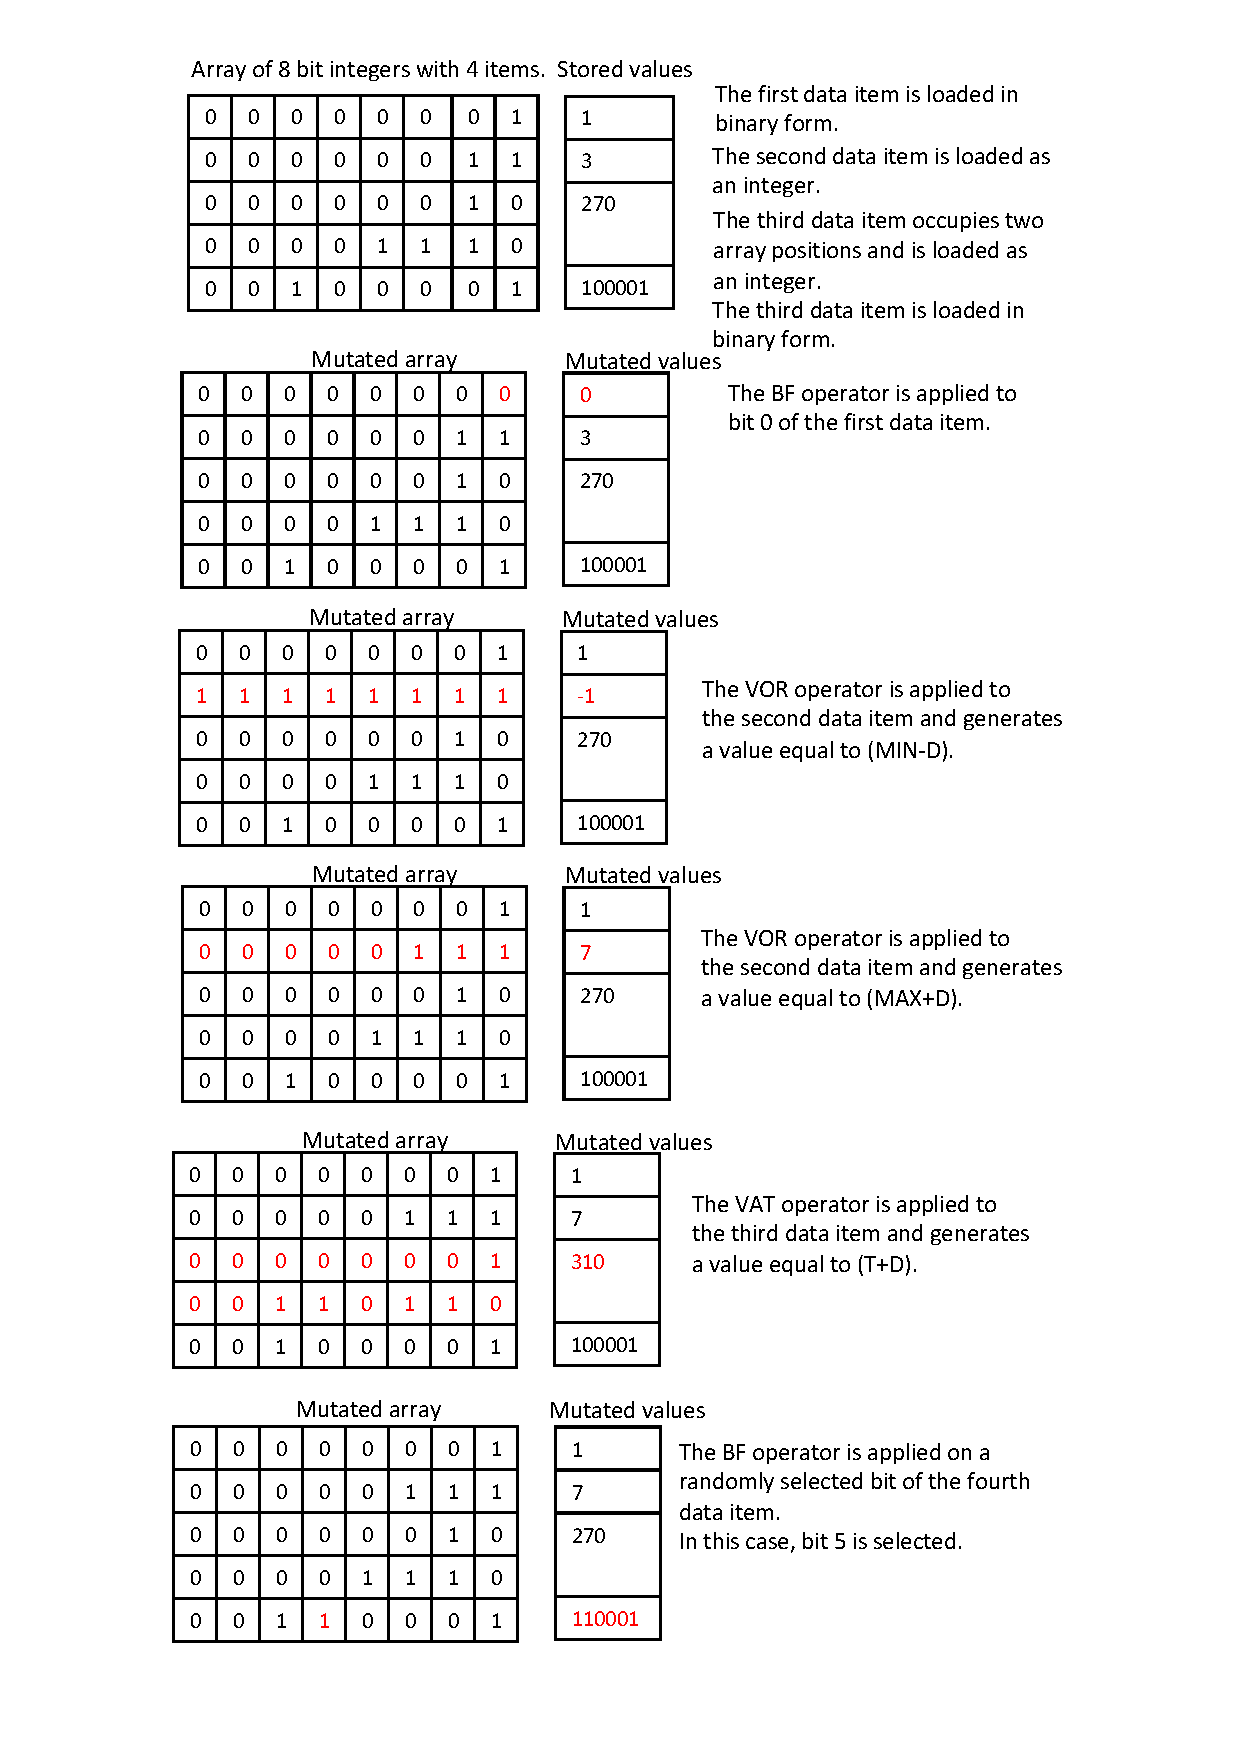
\includegraphics[width=12cm]{images/dataMutationFMExample.pdf}
      \caption{Example of original data and  data mutated according to the fault model in Table~\ref{table:faultModel:example}.}
      \label{fig:dataMutationFMExamples}
\end{figure}





\clearpage


\subsubsection{Automated Generation of Mutation API (Step 2) and Probe Insertion (Step 3)}
\label{sec:generateAPI}

\begin{figure}[tb]
\centering
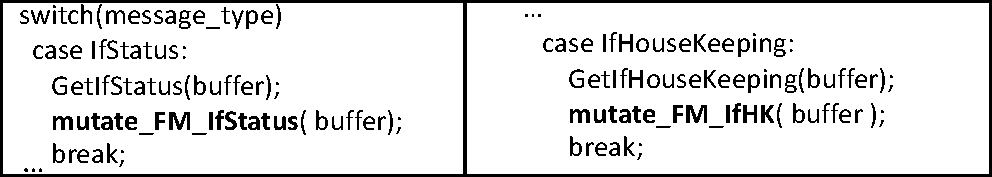
\includegraphics[width=7cm]{damat/images/ProbesExample}
\caption{Example of \APPR mutation probes (in bold).}
\label{fig:appr:ProbesExample}
\end{figure}

\APPR automatically generates a \INDEX{mutation API} to perform mutations at runtime. The API implements a set of functions (called \INDEX{mutate\_FM\_<name>}) that mutate a data buffer according to the given fault model. 
These functions select the data item to mutate and the mutation procedure to apply based on the mutant under test (see Section~\ref{sec:mutantsGeneration}). 

The \APPR mutation API works with C/C++ code; however it may be extended to deal with other programming languages.
Since it is not possible to automatically determine which data buffer to mutate, \APPR requires engineers to modify the source code of the CPS under test by introducing a mutation probe which consists of an invocation of the \APPR function that mutates the data buffer according to a specific fault model.
Note that the effort required by the engineer is minimal; indeed, the exchange of data between components is usually managed in a single location (e.g, the function that serializes the data buffer on the network) and thus it is usually sufficient to introduce one function call for each message type to mutate.
Figure~\ref{fig:appr:ProbesExample} shows how the implementation of \ESAIL has been modified to add the mutation probes. 
The SVF function was modified to handle the message requests sent to the ADCS by inserting one mutation probe for each message type to mutate, e.g., IfStatus and IfHouseKeeping in~Figure~\ref{fig:appr:ProbesExample}. 
Function \emph{mutate\_FM\_IfStatus} is part of the generated mutation API; it loads the fault model \emph{IfStatus} into memory (\UPDATED{our API relies on a tree data structure}) and then invokes the function \emph{mutate}. The function \emph{mutate} performs data-driven mutation according to the provided fault model; the implementation of \emph{mutate} is part of the \APPR toolset.



% At a high-level,
%function \emph{mutate} taking into account the size of the data item; it  checks if the 


The behavior of function \emph{mutate} depends on the value of a unique identifier (i.e., the \emph{MutantID}) associated at compile time to the mutant; the \emph{Mutant ID} univocally identifies the performed mutation operation (each mutant executes one mutation operation, see Section~\ref{sec:mutantsGeneration}).
At a high level, \emph{mutate} performs four activities. First, it checks if the mutation should be performed (i.e., if the data buffer is targeted by the mutation operation identified with the \emph{Mutant ID}). Second, it casts the data item instance targeted by the mutant to a support variable of the type specified in the fault model. Third, it mutates the data stored in the support variable; for each mutation operator, we have implemented a distinct set of instructions for each data representation type. Fourth, before terminating, the function \emph{mutate} writes the mutated data back to the data buffer.





\subsubsection{Automated Generation of Mutants (Step 4)}
\label{sec:mutantsGeneration}



Consistent with code-driven mutation analysis, \APPR generates one mutant for each mutation procedure of the mutation operators configured in the fault model. Each mutant performs exactly one \INDEX{data mutation operation} (i.e., a data mutation procedure configured for a specific data item). For example, the specification in row 6 of Table~\ref{table:faultModel} makes \APPR generate two mutants: each mutant modifies the value of the data item starting at position 12 but one mutant replaces the current value with the value 51 (i.e., $50+1$) while the other replaces the current value with the value $-21$ (i.e., $-20 -1$).

The mutant generation is invisible to the end-user who does not need to modify the source code further; indeed, we rely on a C macro to specify, at compile time, which mutation operation must be performed by every mutant. Mutants are generated by compiling the \UPDATED{SUT} multiple times, once for each mutation operation. At runtime, the mutate function executes only the mutation operation selected for the mutant under test.

\subsubsection{Mutants Execution (Step 5)}
\label{sec:mutantsExecution}

As for \INDEX{code-driven mutation analysis}, the test suite under analysis is executed iteratively with every data-driven mutant. 
At runtime, all the data items targeted by a mutant are mutated whenever the mutation preconditions hold (e.g., the STATE of the BF operator); we leave the mutation of a sampled subset of \UPDATED{data item instances to future work~\cite{zhang2013operator,gopinath2015hard}.}

To speed up the mutation analysis process, the test suite under analysis is first executed with a special mutant that, instead of mutating data items, keeps trace of the fault models loaded by each test case; in other words, it traces what are the data types covered by each test case. The collected information enables the execution, for every mutant, of the subset of test cases that cover the 
message type
%type of data 
targeted by the mutant, thus speeding up mutation analysis.


\subsubsection{Mutation Analysis Results (Step 6)}
\label{sec:mutationAnalysisResults}

Inspired by work on \INDEX{abstract mutation analysis}~\cite{Offutt2006}, we have defined three metrics to evaluate test suites with data-driven mutation analysis: \INDEX{fault model coverage}, \INDEX{mutation operation coverage}, and \INDEX{mutation score}. 
%The first two provide information about the quality of test inputs, whereas the latter provides information about the quality of test oracles \CHANGED{and the test process}. Different from code-driven mutation analysis, data-driven mutation analysis thus enables engineers to distinguish between these two distinct problems affecting test suite effectiveness.
These metrics measure the frequency of the following scenarios: (case 1) the message type targeted by a mutant is never exercised, (case 2) the message type is covered by the test suite but it is not possible to perform some of the mutation operations (e.g., because the test suite does not exercise out-of-range cases), (case 3) the mutation is performed but the test suite does not fail.
\CHANGED{Different from code-driven mutation analysis, these three metrics enable engineers to distinguish between possible test suite shortcomings, including untested message types, uncovered input partitions, poor oracle quality, 
%faulty software, 
and lack of test inputs.}

\INDEX{Fault model coverage (FMC)} is the percentage of fault models covered by the test suite. Since we define a fault model for every 
message type exchanged by two components,
%different data buffer (i.e., type of data exchanged by two components), 
it provides information about the extent to which the message types actually exchanged by the SUT are exercised and verified by the test suites. 
%In other words, low fault model coverage indicates that many test scenarios (e.g., a specific sequence of test inputs being sent to the CPS when the environment is in a specific state) are not exercised by a test suite. 
\CHANGED{Since different component functionalities often require different message types, low fault model coverage may indicate that only a small portion of the integrated functionalities have been tested.}

\INDEX{Mutation operation coverage (MOC)} is the percentage of data items that have been mutated at least once, considering only those that belong to the data buffers covered by the test suite. It provides information about the input partitions covered for each data item; for example, the FVOR operator leads to two mutation operations, which are applied only if the observed value is outside range. Otherwise the two mutation operations will not be covered, thus enabling the engineer to identify such shortcoming in the test suite.
%TODO: add example

The \INDEX{mutation score (MS)} is the percentage of mutants killed by the test suite \UPDATED{(i.e., leading to at least one test case failure)} among the mutants that target a fault model and for which at least one mutation operation was successfully performed. It provides information about the quality of test oracles; indeed, a mutant that performs a mutation operation and is not killed (i.e., is \emph{live}) indicates that the test suite cannot detect the effect of the mutation (e.g., the presence of warnings in logs).
% or an unexpected output from the system). 
\CHANGED{Also, a low mutation score may indicate missing test input sequences. Indeed, live mutants may be due to either software faults (e.g., the SUT does not provide the correct output for the mutated data item instance) or the software not being in the required state (e.g., input partitions for data items are covered when the software is paused); in such cases, with appropriate input sequences, the  test suite would have discovered the fault or brought the SUT into the required state. Both poor oracles and lack of inputs indicate flaws in the test case definition process (e.g., the stateful nature of the software was ignored).}

\clearpage
\subsection{Running Examples}
\label{sec:dataDriven:example}

In this Section, we provide a set of running examples that show the results achieved by \APPR in the presence of test suites affected by different problems. More precisely we aim to demonstrate, for representative cases, the absence of false alarms due to equivalent mutants and the usefulness of the mutation analysis metrics computed. 
\REVTOOL{P-3}{Each running example is an artificial but realistic definition of test suites to illustrate the methodology.}
We consider the following representative scenarios:
\begin{enumerate}
\item The test suite exercises only one message exchange between the ADCS and the SUT; each test case covers a distinct input partition.
\item The test suite exercises only one message exchange between the ADCS and the SUT; multiple test cases cover a same input partition.
\item The test suite exercises multiple message exchanges between the ADCS and the SUT; each test case covers a distinct combination of input partitions.
\end{enumerate}


\subsubsection{Example set 1: One message exchange, distinct input partitions}
\label{sec:dataDriven:example:1}

\begin{figure}[tb]
\centering
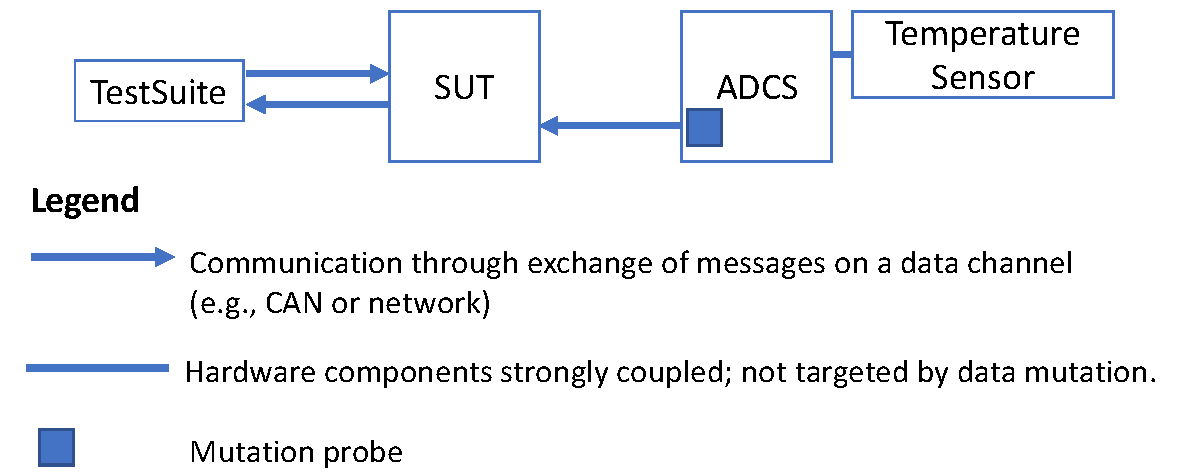
\includegraphics[width=8cm]{damat/RunningExampleArch}
\caption{Architecture of the running example system.}
\label{fig:damat:RunningExampleArch}
\end{figure}

Our first set of running examples concerns the presence of a single message exchange and test cases covering distinct input partitions.

Our examples concern an SUT that exchanges with the ADCS component one type of message. More precisely, the ADCS sends a message (hereafter, \emph{TempMessage}) with the temperature collected by its sensor. The architecture of such system is shown in Figure~\ref{fig:damat:RunningExampleArch}. For simplicity, we assume that the ADCS periodically sends a TempMessage to the SUT. The ADCS is connected to the TemperatureSensor. The communication between the ADCS and the TemperatureSensor is not affected by data-driven mutation. We may assume the ADCS and the TemepratureSensor are simulated during the execution of the test suite. The SUT and the ADCS communicate through a channel 
(e.g., a CAN bus). The data mutation probe is inserted in the ADCS simulator; in practice we mutate the data generated by the ADCS. The test suite exercises the software under test by communicating through a data channel; the type of communication channel used by the test suite is not relevant for the purpose of the running example.

For our running example, the SUT has two state variables that are observable by the test suite, \emph{temperature} and \emph{temperature\_alarm}. The state variable \emph{temperature} reports the temperature returned by the sensor in the last message. 
The state variable \emph{temperature\_alarm} is set to 1 if the temperature returned by the sensor is above 100.

The test suite is comprised of two test cases. \emph{Test 1} exercises the SUT with a temperature in the nominal case (i.e., temperature below 100), \emph{Test 2} concerns the non nominal case (i.e., temperature above 100). The two test cases of the test suite exercise the same sequence of interactions, which are depicted in the UML Sequence diagram of Figure~\ref{fig:damat:RunningExample1Sequence}. The sequence diagram shows that the test case first starts the ADCS simulator and the SUT; then, it waits for the ADCS to send the TempMessage before requesting the values of the variables \emph{temperature} and \emph{temperature\_alarm}. Figure~\ref{fig:damat:RunningExample1Sequence} also shows that, in this case, the mutation is performed within the ADCS simulator.

\begin{figure}[tb]
\centering
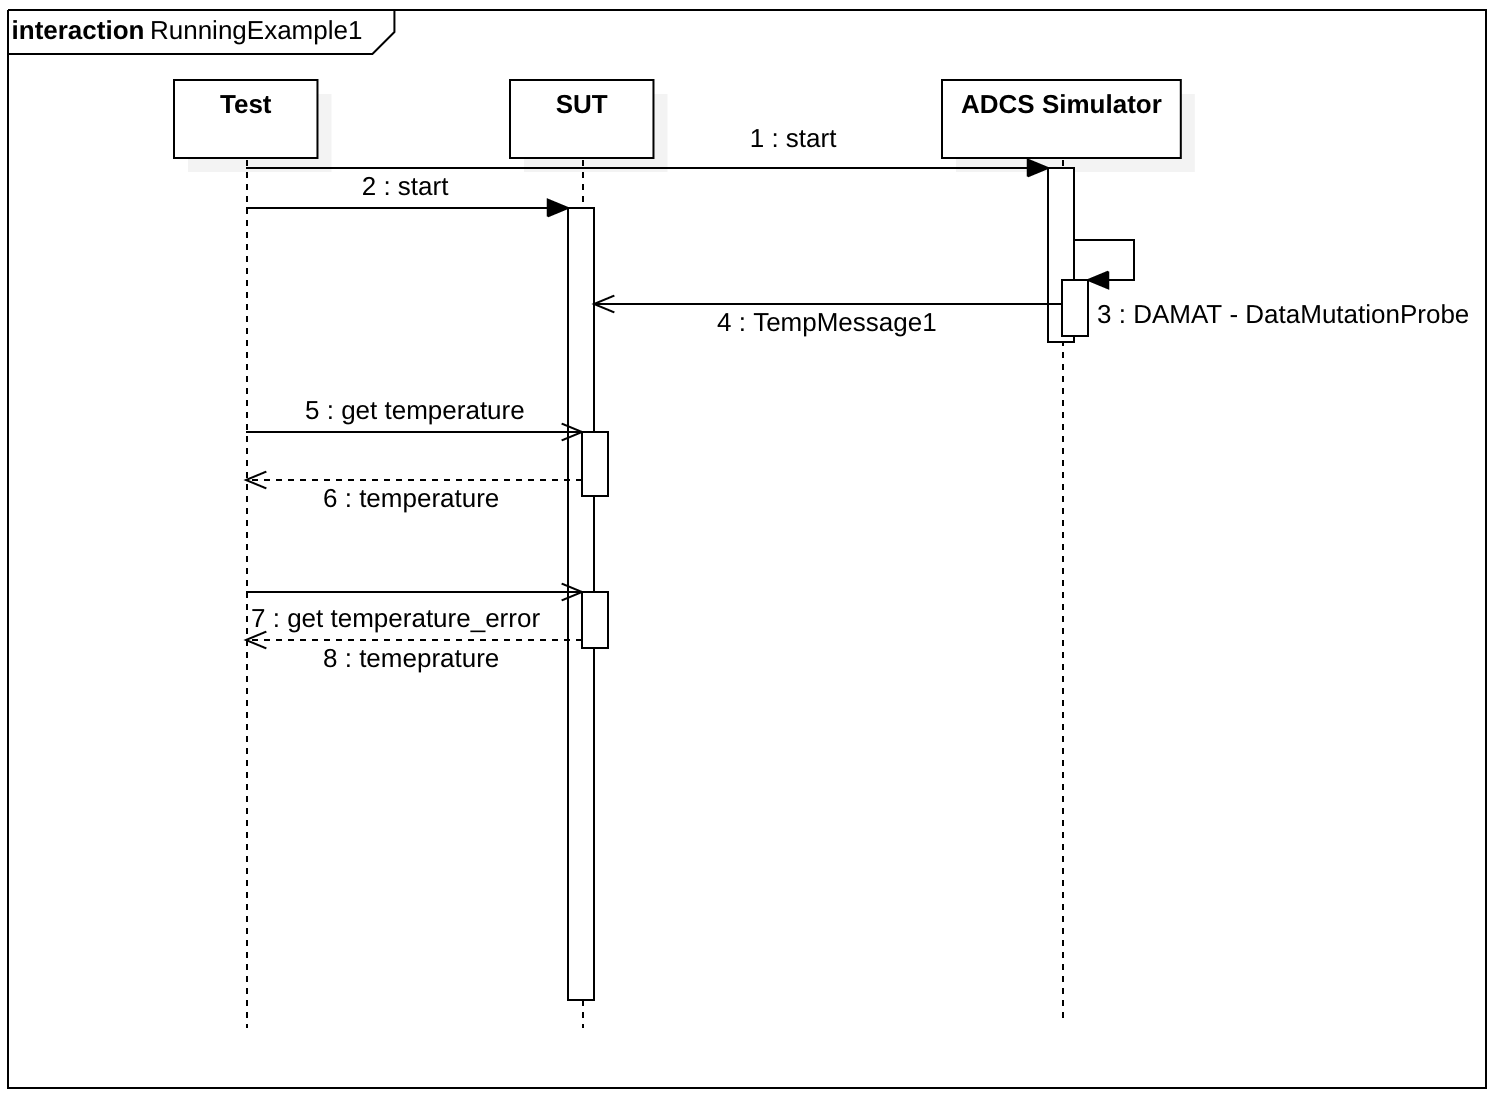
\includegraphics[width=8cm]{damat/images/runningExamplesSequence1.png}
\caption{Interactions exercised by the test cases belonging to the running example set 1.}
\label{fig:damat:RunningExample1Sequence}
\end{figure}


Figures~\ref{fig:damat:RunningExample1A} to~\ref{fig:damat:RunningExample1C} show our running examples. On the top, we report the fault model. In this case the fault model applies the operators VAT (value above threshold) and FVAT (fix value above threshold). The VAT operator is configured with a threshold of 100 and a delta of 10 (i.e., it replaces values below the threshold with the value 110). The FVAT operator is configured in the same manner (i.e., it replaces values above threshold with the value 90). The operator VAT leads to \emph{MUTANT 1}, the operator FVAT leads to \emph{MUTANT 2}; \REVTOOL{P-5}{to summarize, in this example we have two mutants, each implements one distinct mutation operator.}

In Figure~\ref{fig:damat:RunningExample1A}, under \emph{Exchanged data}, we report the sequence of data messages exchanged by the test cases of the test suite (one column for each test case).
In the following rows, we report the oracles. For each oracle we indicate how it verifies if a state variable has been assigned with a correct value; we indicate $"=="$ if it verifies the exact value taken by the state variable (e.g., \emph{temperature == 50)}, "$>=$" if it verifies that the value is above a threshold (e.g., \emph{temperature $>=$ 50}). Please note that, according to standard practice, test cases for non nominal cases verify that state variables contain the expected alarm and anomalous values (i.e., the test case passes only if the SUT report the anomaly). 

For each mutant, we report the value of the data exchanged during the execution and the data of the state variables read by the oracle. In red we indicate data that has been mutated according to the fault model. 
If an oracle does not read the value of a variable we leave the cell empty.
Failing oracles are highlighted in yellow.
\REVTOOL{P-5}{Note that for each mutant we provide multiple columns (named \emph{Test 1} and \emph{Test 2}), each provides the data exchanged during the execution of the test case.}
Finally, for each mutant, for each oracle, we report the test cases that detect the anomalous value (if any); also, we report if the mutant had been killed.


Please note that, following the \APPR procedures, MUTANT 1 does not mutate the data exchanged by Test 2 because it is already above the threshold. MUTANT 2 does not mutate the data exchanged by Test 1 because it is already below the threshold.

TestSuite1 is an optimal test suite that verifies the expected value of all the state variables. For MUTANT 1, Test 1 fails because the assertion about temperature fails (expected 50 observed 110).
For MUTANT 2, Test 2 fails because the assertion about temperature fails (expected 120 observed 90).
\REVTOOL{P-6}{We have a fault model coverage (\emph{FMC}) of 100\% because we have only one fault model and it is covered (i.e., the test suite exchanged the data message under analysis). We have a mutation operator coverage (\emph{MOC}) of 100\% because all the mutation operations associated with the configured mutation operators are applied (in other words, all the mutants perform at least one mutation of a data item instance). We have a mutation score (\emph{MS}) of 100\% because, for each mutant, at least one test case fails.}

TestSuite2 verifies the expected value of the temperature for the nominal case and the presence of a temperature error for the non nominal case. For MUTANT 1, Test 1 fails because the assertion on temperature fails (expected 50 observed 110).
For MUTANT 2, Test 2 fails because the assertion on temperature errors fail (expected 1 observed 0).
\REVTOOL{P-6}{Concerning FMC, MOC, and MS, the same considerations made for TestSuite1 hold.}

TestSuite3 verifies only temperature values while TestSuite4 verifies only temperature alarms. They all kill the mutants for the same reasons reported in the cases above. \REVTOOL{P-6}{Concerning FMC, MOC, and MS, the same considerations made for TestSuite1 hold.}


TestSuite5 is a copy of TestSuite2 having an imprecise oracle (i.e., it verifies that temperature is above 50 instead of equal to 50). Consequently the test suite does not fail for MUTANT 1 and the mutation score is not 100\%; consequently, \APPR enables an engineer to detect the limitation of the test suite.

\REVTOOL{P-6}{TestSuite6} is a copy of TestSuite2 without an oracle for Test2 (i.e., it does not verify the presence of temperature alarms). Consequently, the test suite does not fail for MUTANT 2 and the mutation score is not 100\%; consequently, \APPR enables an engineer to detect the limitation of the test suite.

TestSuite7 is a copy of TestSuite2 with multiple test cases covering the same input partitions; indeed, Test3 covers the same input partition of Test1 (i.e., it exercises the value 0, which is a nominal value like 50), Test4 covers the same input partition of Test2 (i.e., it exercises the value 101, which is a non nominal value like 120). All the mutants are killed by the test suite and we do not observe equivalent mutants.

TestSuite8 is a copy of TestSuite7 with the same limitations of TestSuite6 (i.e., Test2 does not contain an oracle).
In this case, the mutation score is 100\% because Test 4 contains an appropriate oracle and covers the same input partition not appropriately verified by Test 2. We do not observe equivalent mutants.

TestSuite9 is a copy of TestSuite7 without oracles for both Test2 and Test4; similarly to the case of TestSuite6, since the non-nominal partition is not appropriately verified, the mutation score is not 100\%; consequently, \APPR enables an engineer to detect the limitation of the test suite.

TestSuite10 covers the case of a test suite that does not exercise an input partition; precisely, it does not exercise non nominal values. 
In this case, \APPR can detect that MUTANT 2 is never applied (to exemplify it, we do not report any red value for MUTANT 2 in Figure~\ref{fig:damat:RunningExample1C}); consequently, the MOC is not 100\% and the engineer can determine what is the limitation of the test suite. Indeed, since the mutant not covered is FVAT, the engineer can know that the test suite does not exercise the value above threshold for the temperature (FVAT applies the mutation only if a value above threshold is observed).

\begin{figure}[tb]
\centering
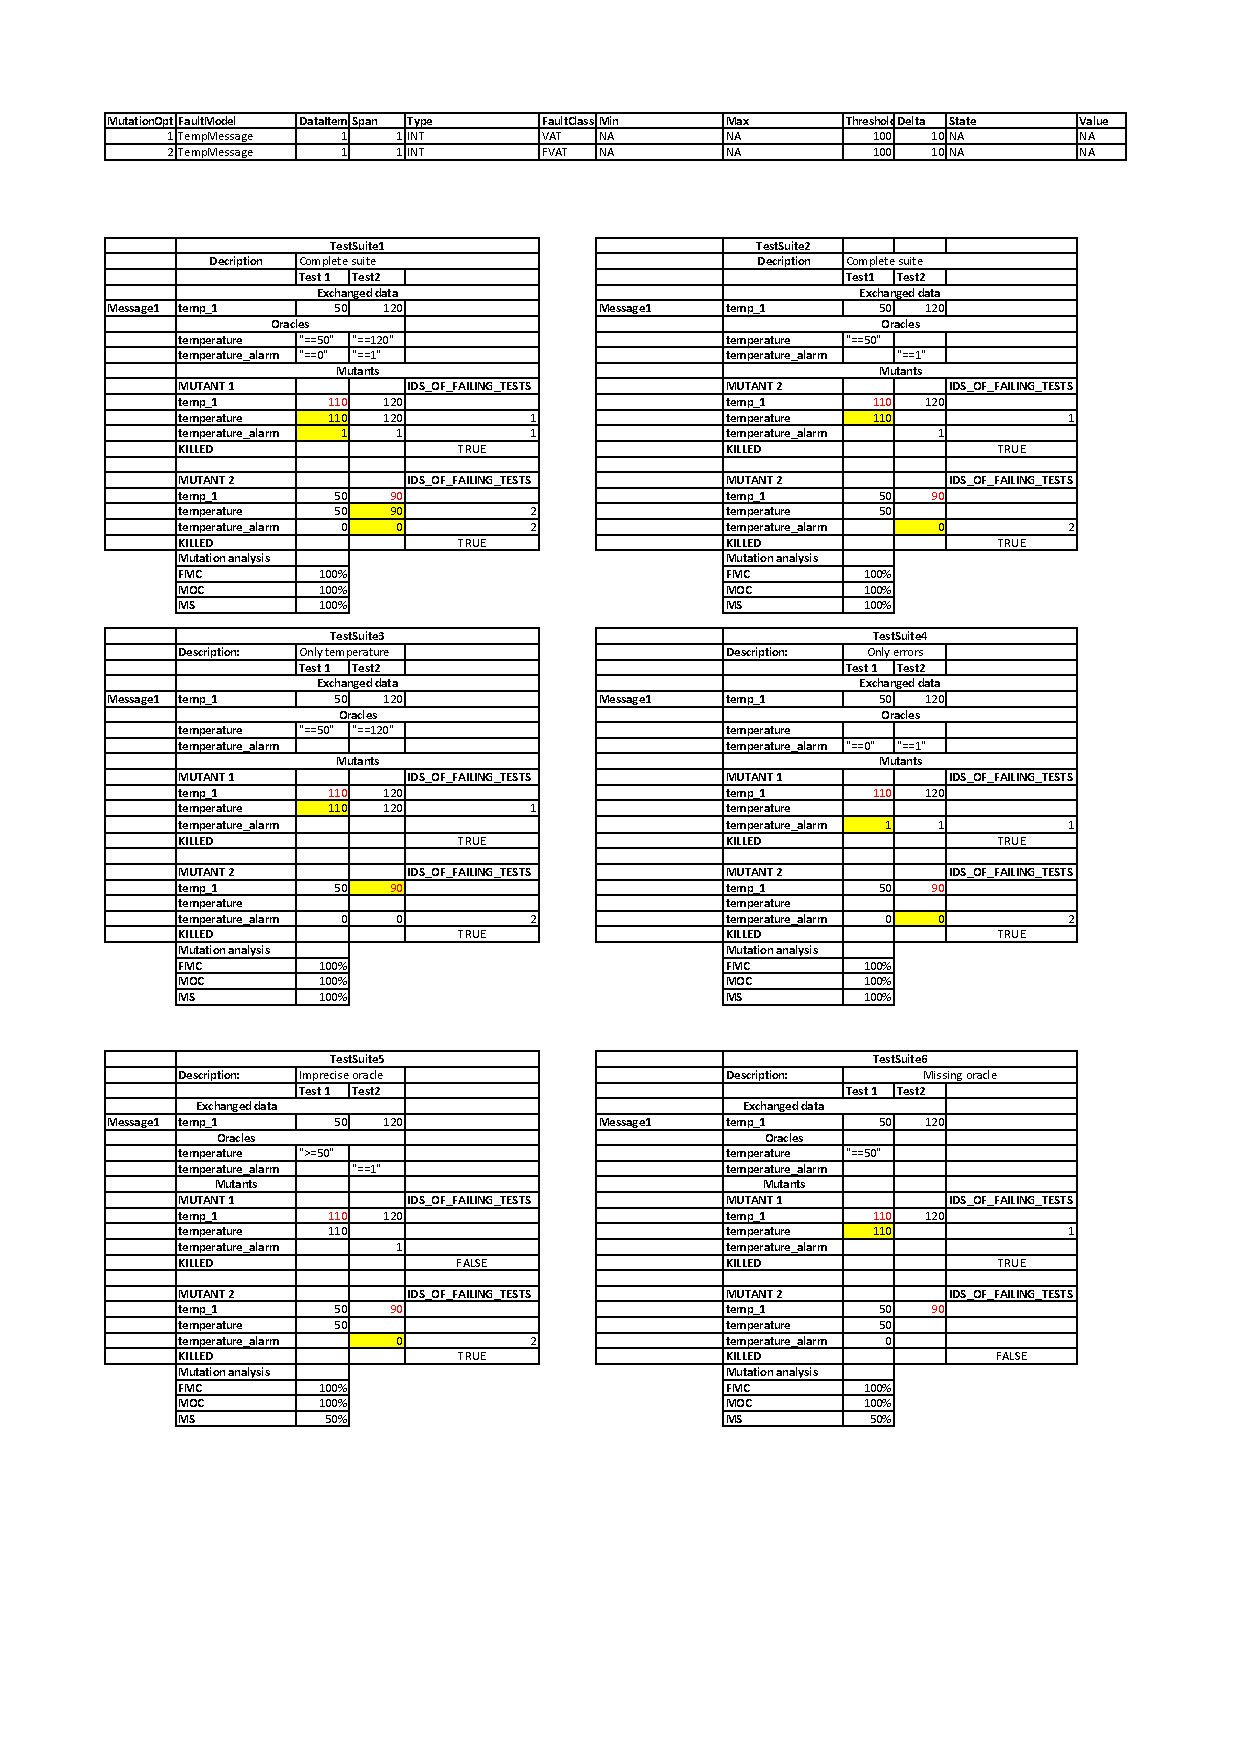
\includegraphics[width=18cm]{damat/DataDrivenExample1A}
\caption{Running example set 1 - Part A.}
\label{fig:damat:RunningExample1A}
\end{figure}

\begin{figure}[tb]
\centering
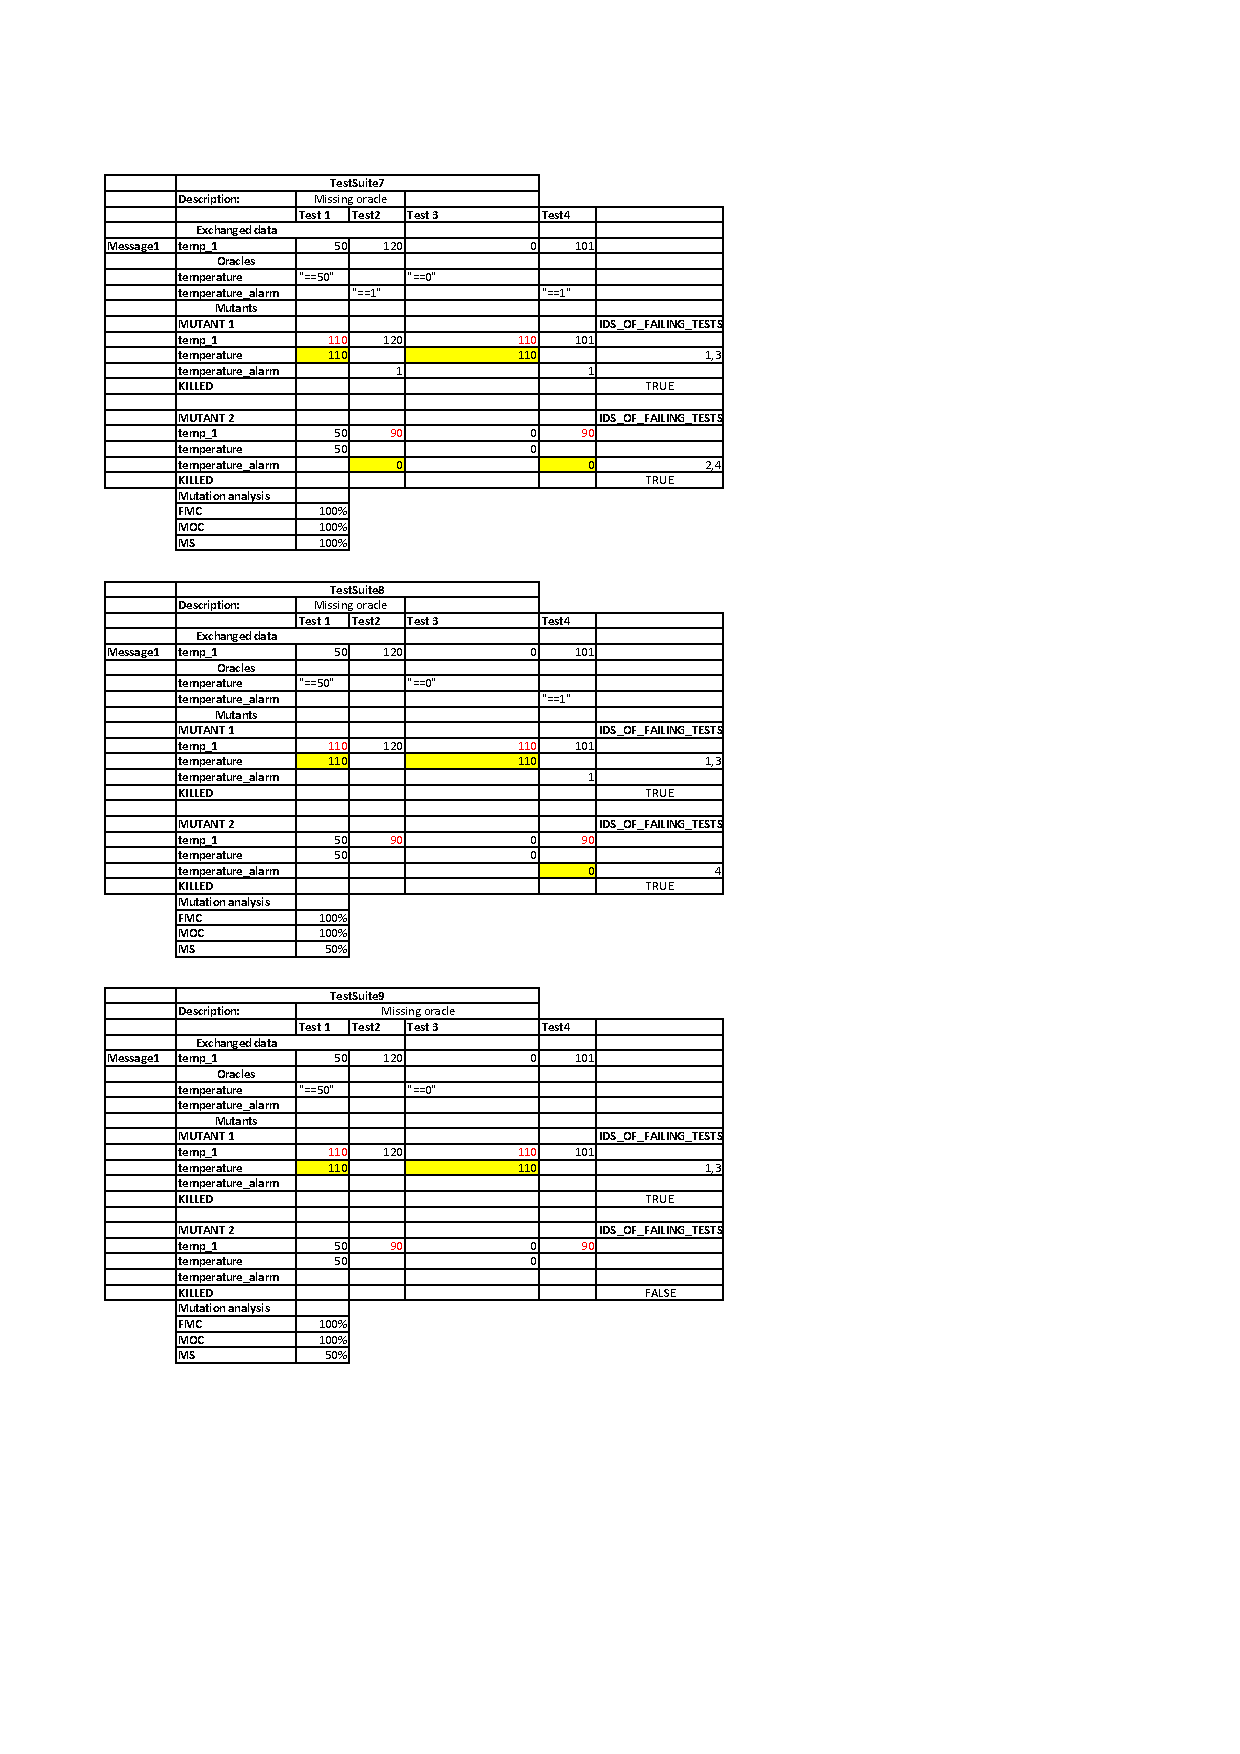
\includegraphics[width=18cm]{damat/DataDrivenExample1B}
\caption{Running example set 1 - Part B.}
\label{fig:damat:RunningExample1B}
\end{figure}

\begin{figure}[tb]
\centering
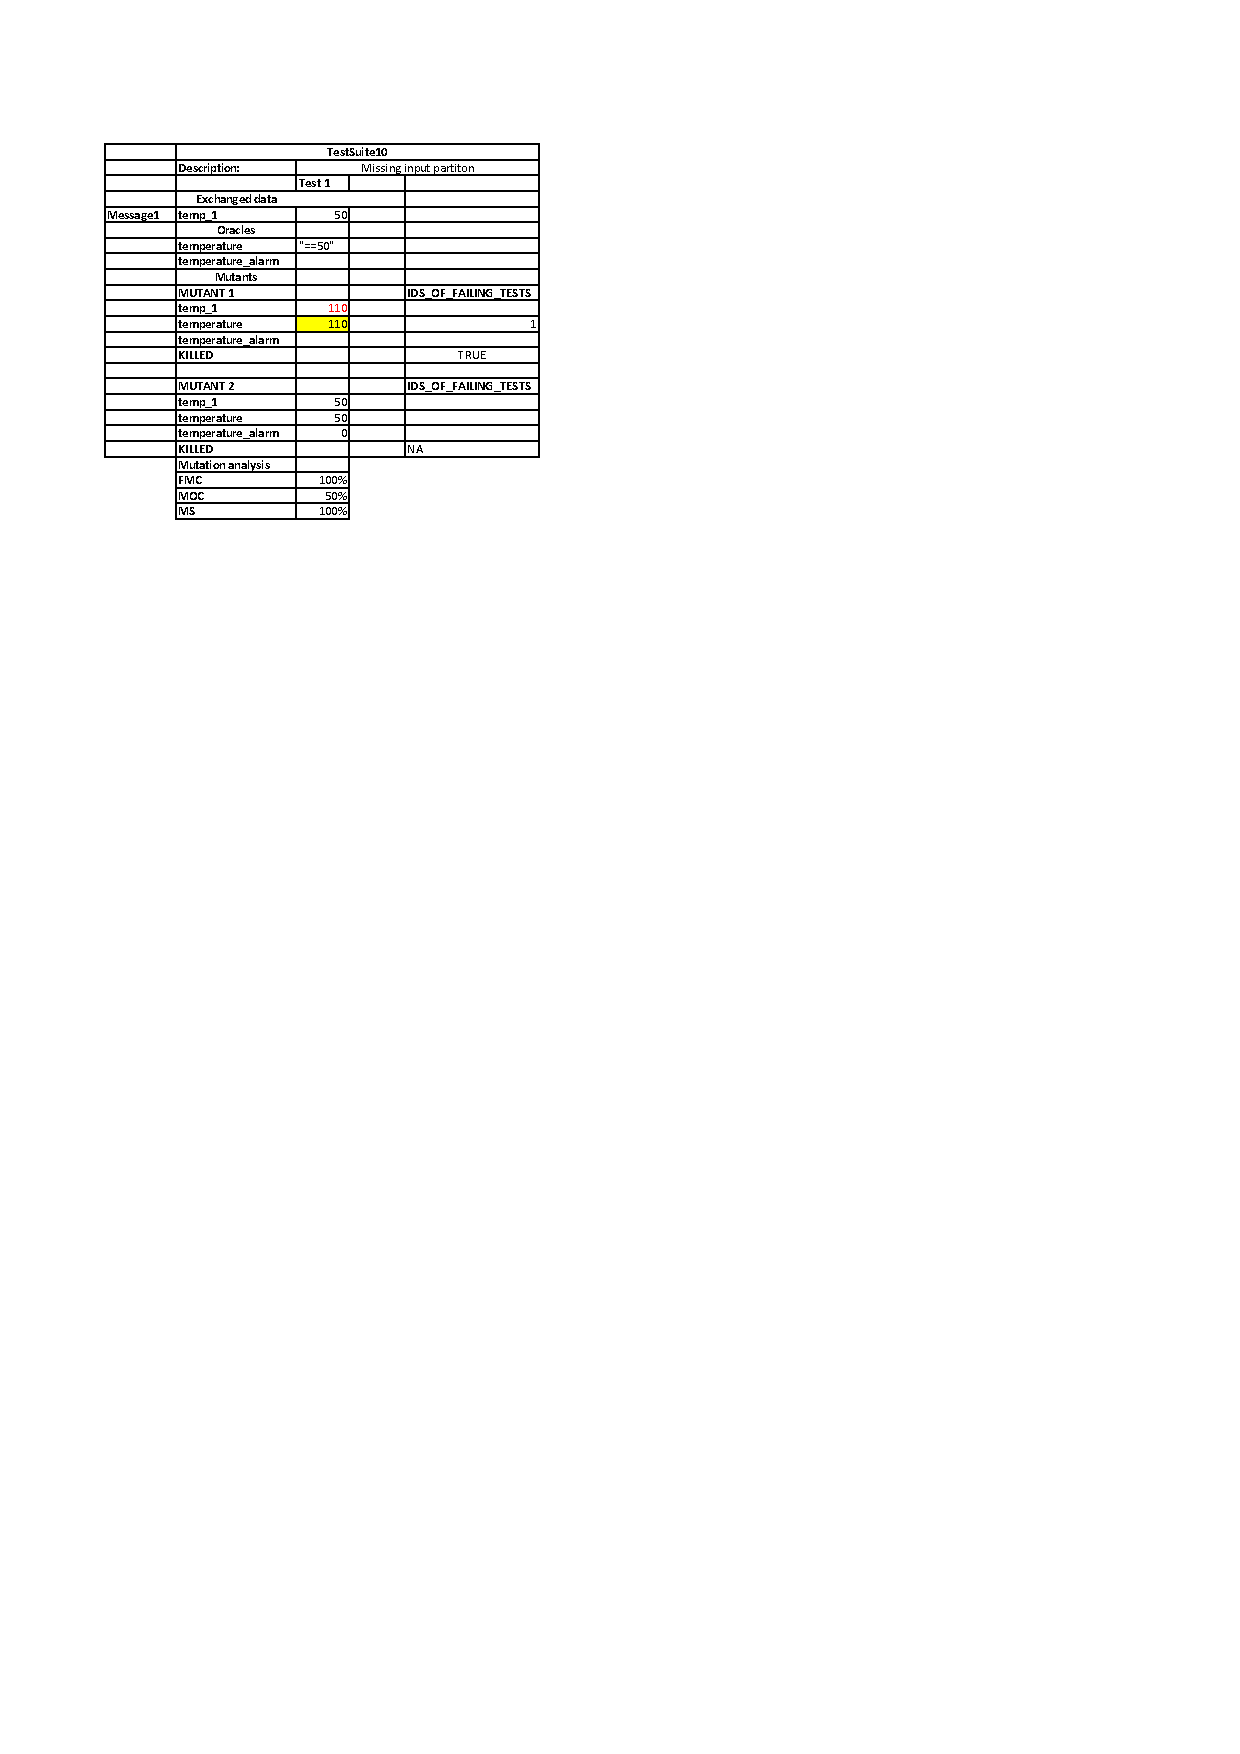
\includegraphics[width=18cm]{damat/DataDrivenExample1C}
\caption{Running example set 1 - Part C.}
\label{fig:damat:RunningExample1C}
\end{figure}

%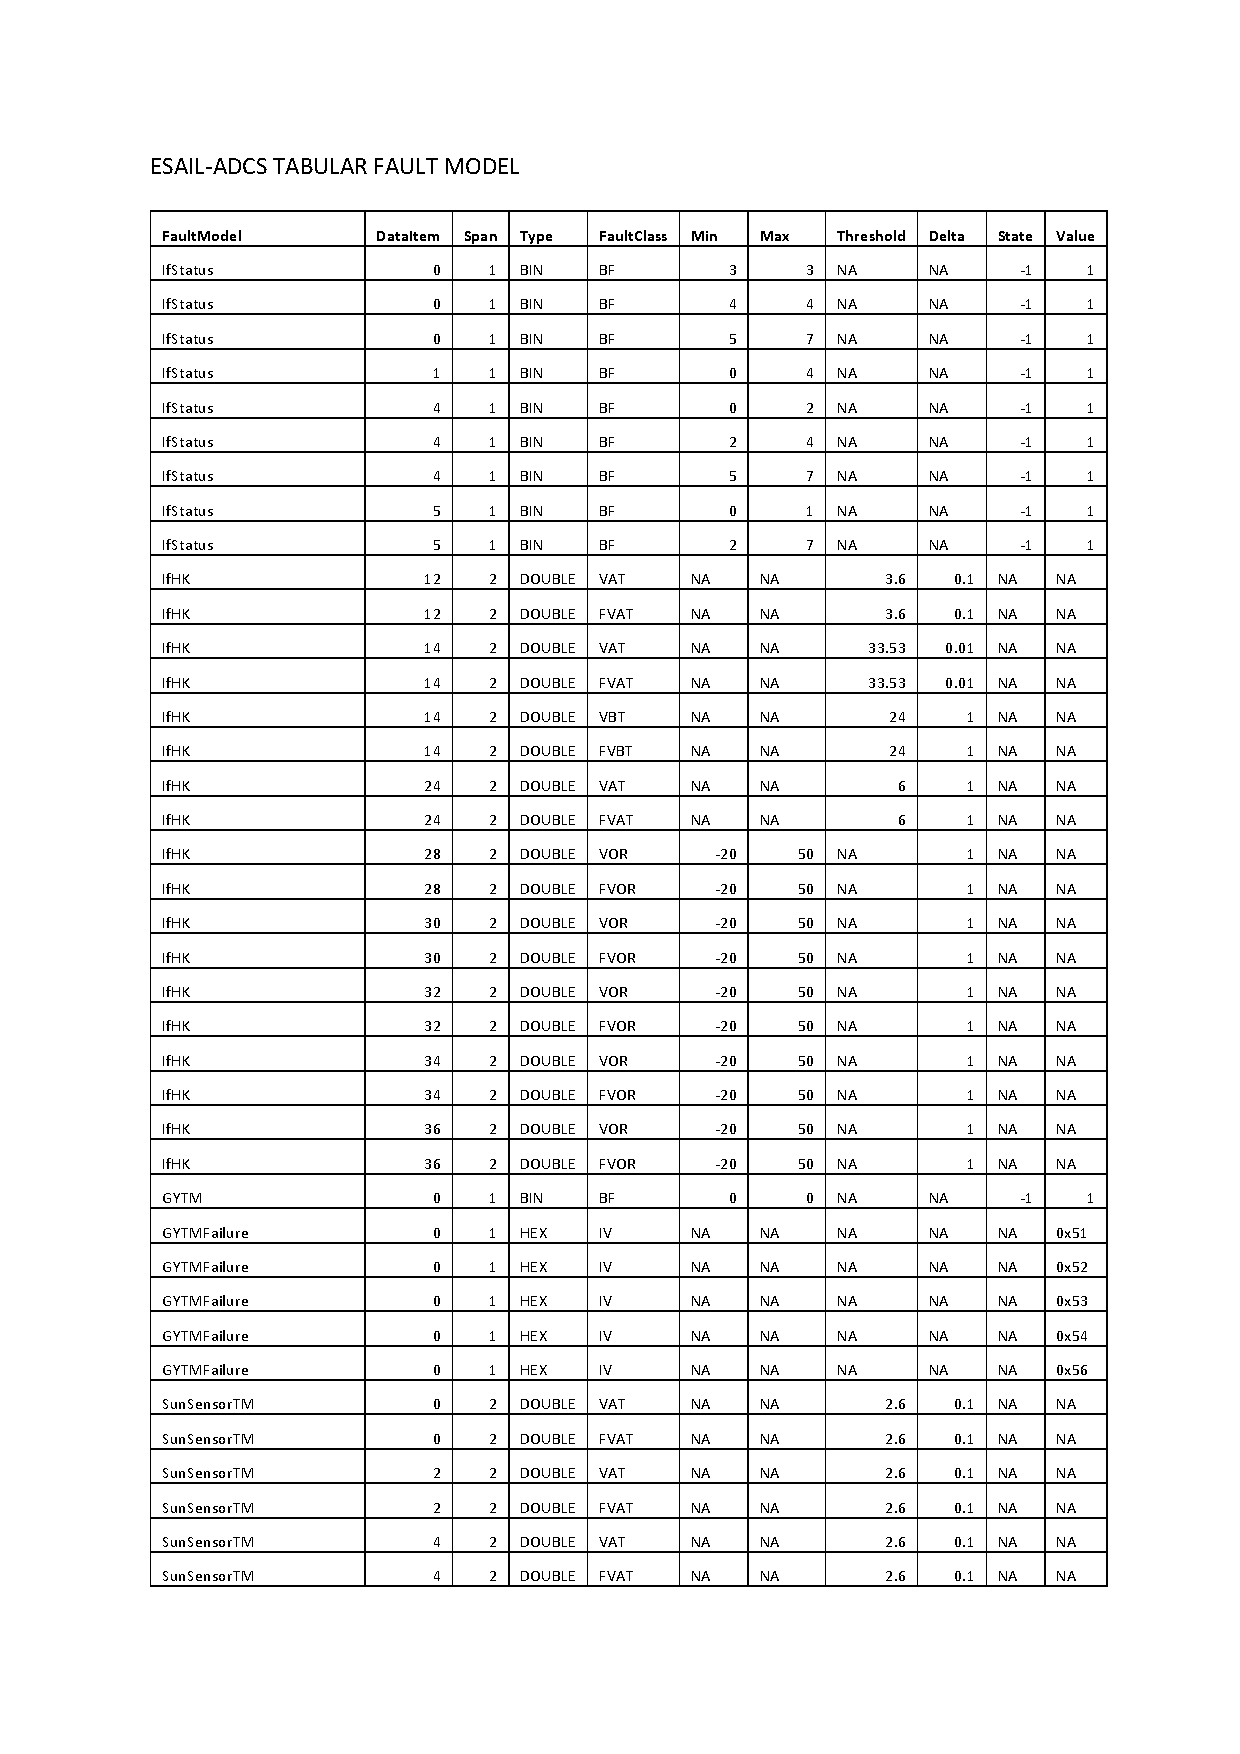
\includepdf[pages=-,scale=0.9,offset=0mm -75]{faultModels/FaultModels.pdf}

\clearpage

\subsubsection{Example set 2: One message exchange, distinct input partitions, faulty software}
\label{sec:dataDriven:example:2}

This running example (see Figure~\ref{fig:damat:RunningExample2}) covers the same case of Section~\ref{sec:dataDriven:example:1}, with the difference that we assume the software to be faulty. More precisely, we assume that the value of \emph{temperature alarm} is always set to 0. We ignore the test suites number 1, 2, 4, 5, 6, 7, 8 because they would detect the presence of the fault before mutation analysis (i.e., the oracles "==1" would fail). For completeness, in Figure~\ref{fig:damat:RunningExample2}, we report the values of state variables also when they are not verified by oracles. We highlight failing oracles in yellow.

For TestSuite6 and TestSuite9, which do not detect the fault because they lack an oracle for the faulty variable, \APPR would indicate that MUTANT 2 is not killed thus enabling the engineer to introduce an appropriate oracle (i.e., "temperature\_alarm == 1") and thus discover the fault. 

For TestSuite3, \APPR would not help the engineer in detecting the fault because the test suite kills the mutant. What we observe in this case is a sort of masking effect due to the fact that two outputs are affected by the same data; indeed, \APPR ensures that the effect of data mutation is propagated to at least one software output but it cannot verify that the effects of data mutation are propagated to all the software outputs that depend on the mutated data. 
%In this specific case, we would like to highlight that a correct test case would have verified first the presence of temperature_alarms. 
%For the detection of algorithmic faults, code-driven mutation analysis might be more appropriate.

\begin{figure}[tb]
\centering
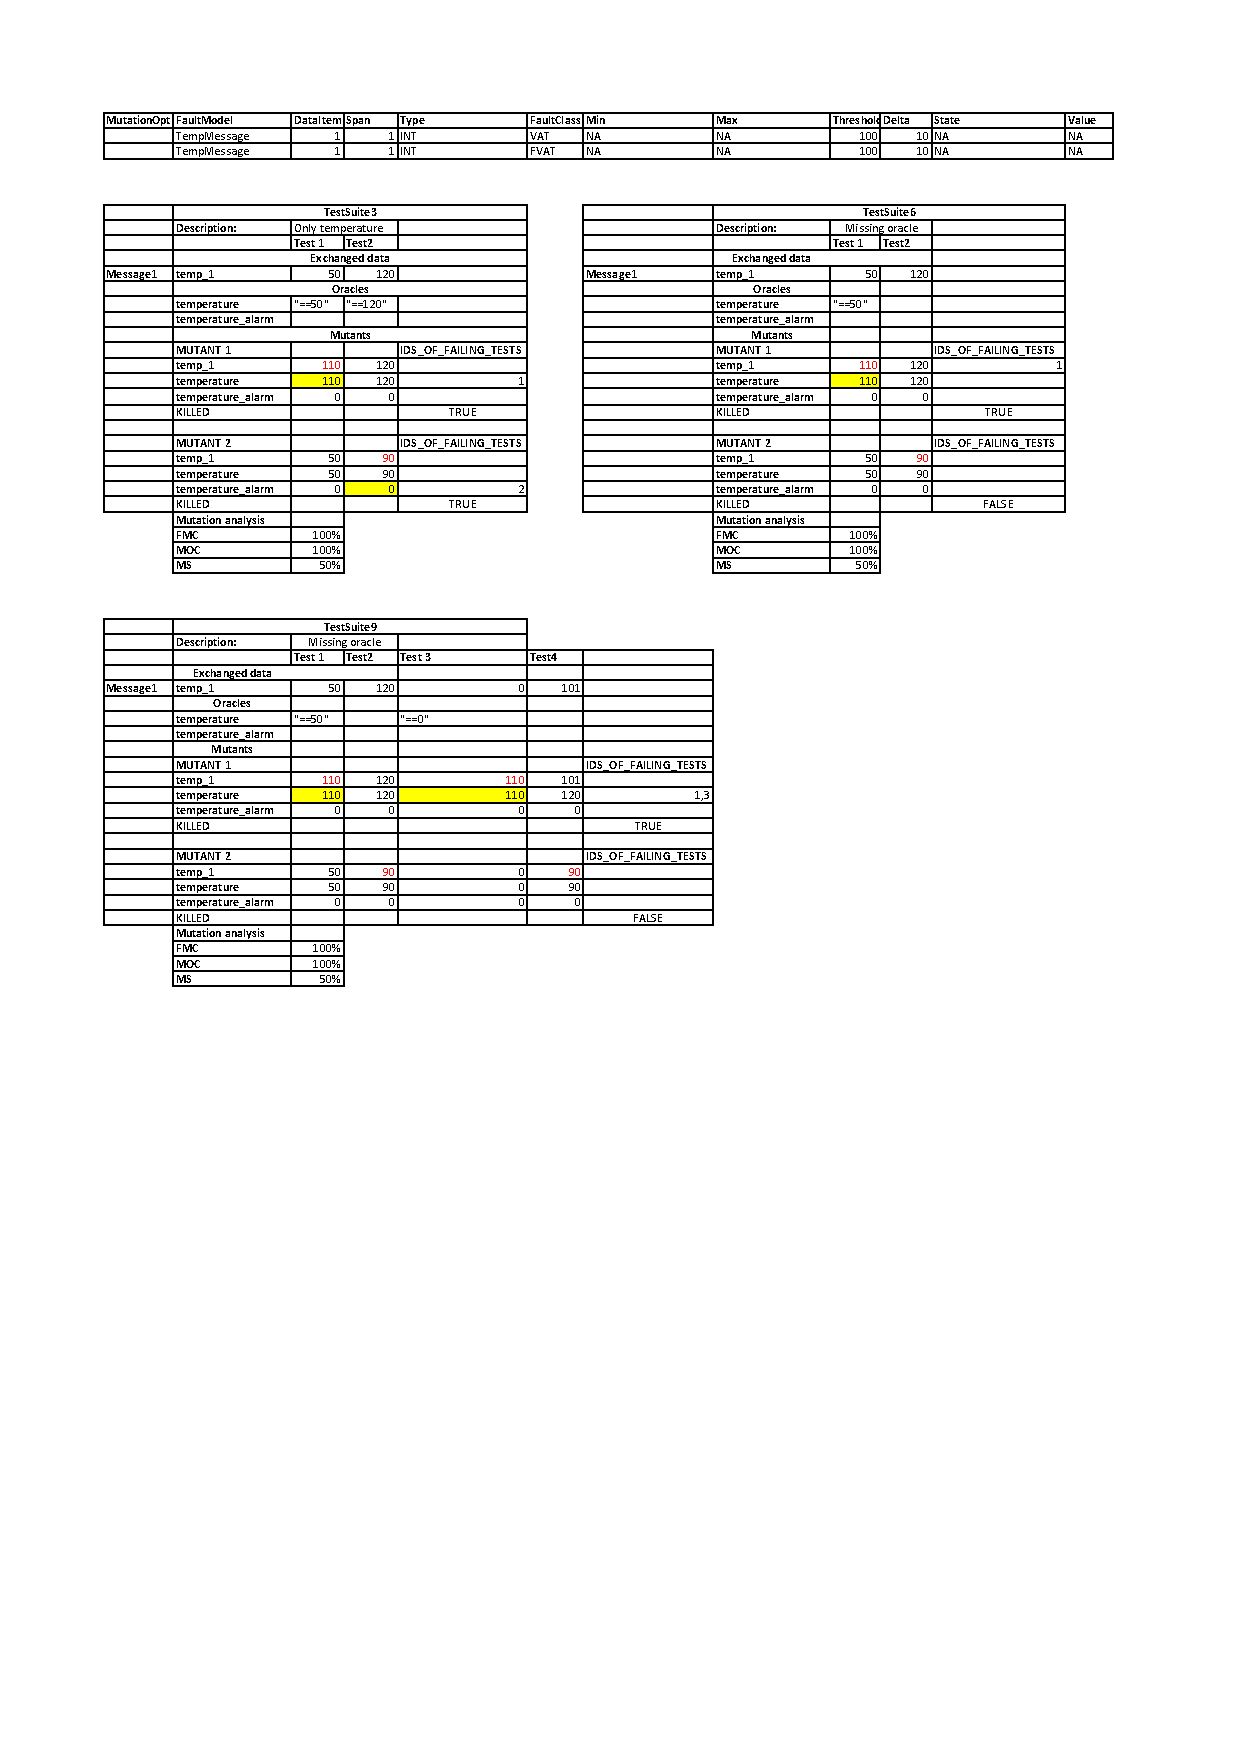
\includegraphics[width=14cm]{damat/DataDrivenExample2}
\caption{Running example set 2.}
\label{fig:damat:RunningExample2}
\end{figure}

\clearpage 
\subsubsection{Example set 3: Multiple message exchanges, distinct input partitions}
\label{sec:dataDriven:example:3}

For the third running example set, we consider a system that has the same architecture of  Figure~\ref{fig:damat:RunningExampleArch} but exchanges also messages of type \emph{BoardStatus}. We assume that \emph{BoardStatus} messages indicate the voltage of the board and the sensors. The SUT has an additional output state variable called \emph{voltage\_error}. A voltage error occurs when the voltage is out of the range (10;14). In the presence of a voltage error, the software shall not update the value of the \emph{temperature} state variable.

Below we discuss two possible test suites, TestSuite1 and TestSuite2, which are affected by different type of limitations.
More precisely, we rely on TestSuite1 to (1) show how \APPR spot a test suite shortcoming difficult to determine manually and (2) demonstrate that \APPR may unlikely lead to equivalent mutants (i.e., by showing that if a mutant is not killed it's because relevant assertions are missing). We rely on TestSuite2 to exemplify the case of lack of coverage of a fault model.

\paragraph{TestSuite1}

Figure~\ref{fig:damat:RunningExample3Sequence} shows the interactions exercised by the test cases in the test suite named TestSuite1 for the running example set 3. Each test case, after starting the ADCS simulator and SUT, waits till the ADCS has sent the following sequence of messages: one BoardStatus message, one TempMessage, one BoardStatus message, and one TempMessage. Then it requests and verifies the values of the state variables \emph{temperature}, \emph{temperature\_alarm}, and \emph{voltage\_error}.

\begin{figure}[tb]
\centering
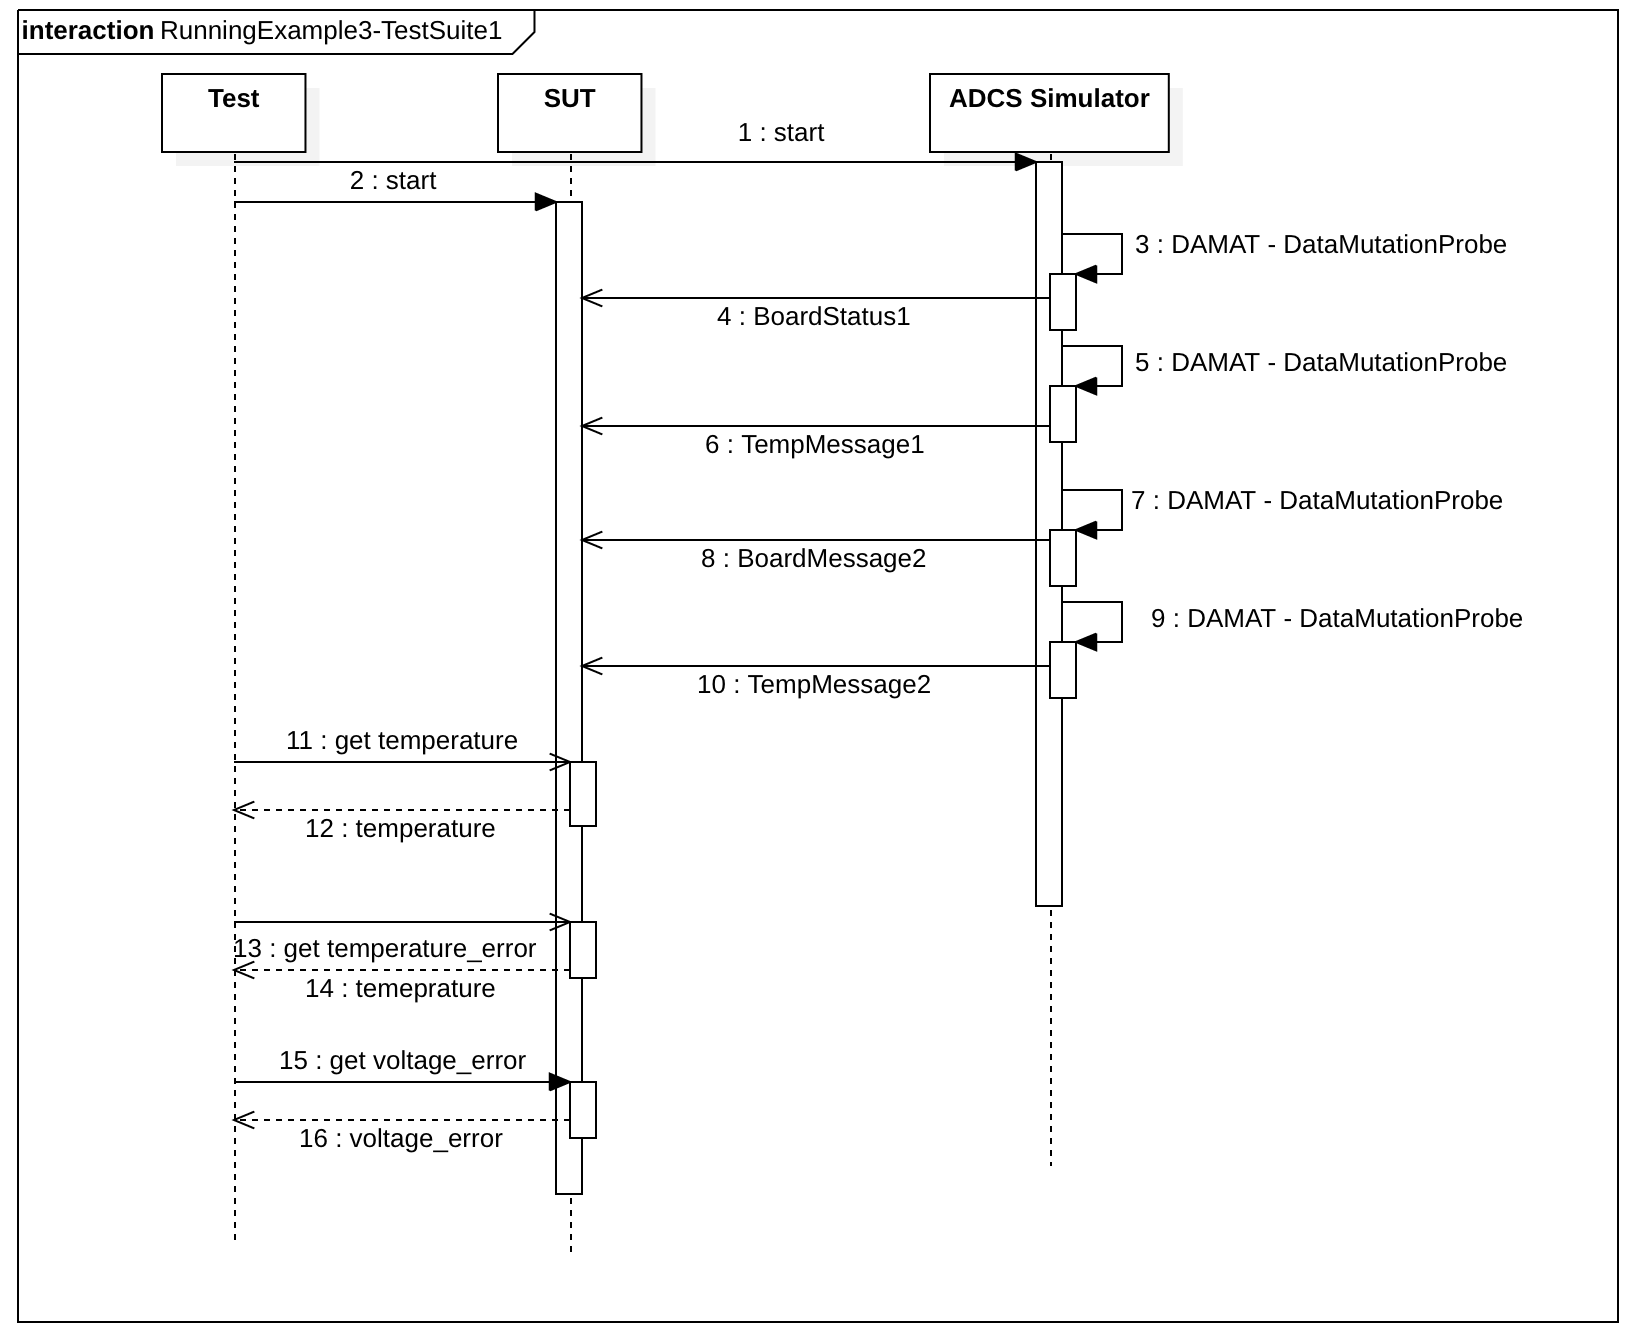
\includegraphics[width=8cm]{damat/images/RunningExampleSequence3.png}
\caption{Interactions exercised by the test cases of TestSuite1 in the running example set 3.}
\label{fig:damat:RunningExample3Sequence}
\end{figure}

Figures~\ref{fig:damat:RunningExample3A} and~\ref{fig:damat:RunningExample3B} show the data exchanged in our running example. With respect to the example set 1, the fault model includes also one VOR and FVOR operator to mutate the BoardStatus message. In Figures~\ref{fig:damat:RunningExample3A} and~\ref{fig:damat:RunningExample3B}, in the row named \emph{PASS}, we explicitly indicate the result of each test case (i.e., PASS or FAIL).

TestSuite1 covers all the possible combinations of values for the sequence of messages reporting about messages voltage error absent (true or false), temperature alarm absent (true or false), voltage error absent (true or false), temperature alarm absent (true or false); indeed, in total, we have 16 test cases.

TestSuite1 kills MUTANT 1. MUTANT 1 applies VAT, that is, it sets the temperature value above the threshold when it is below the threshold. To not kill MUTANT 1, the test suite should not include any failing oracle. Since the failing oracles include the complete set of oracles that either verify the temperature being in the nominal range or verify the absence of a temperature alarm, we conclude that whenever MUTANT 1 is not killed, we cannot be in the presence of an equivalent mutant but in the presence of a test suite limitation.

TestSuite1 kills MUTANT 2. MUTANT 2 applies FVAT, that is, it sets the temperature value below the threshold when it is above the threshold. To not kill MUTANT 2, the test suite shall not include any of the failing oracles. Since the failing oracles include the complete set of oracles that either verify the temperature being out of the nominal range or verify the presence of a temperature alarm, we conclude that whenever MUTANT 2 is not killed, we cannot be in the presence of an equivalent mutant but in the presence of a test suite limitation.

TestSuite1 kills MUTANT 3. MUTANT 3 applies the first mutation procedure of VOR, that is, it sets the value above range if it is within range. To not kill MUTANT 2, the test suite shall not include any of the failing oracles. Since the failing oracles include the complete set of oracles that either verify the temperature being in the nominal range or verify the absence of a temperature alarm, we conclude that whenever MUTANT 3 is not killed, we cannot be in the presence of an equivalent mutant but in the presence of a test suite limitation.

TestSuite1 kills MUTANT 4. MUTANT 4 applies the second mutation procedure of VOR, that is, it sets the value below range if it is in range. MUTANT 4 leads to the same system outputs as MUTANT 3 thus we can make the same conclusion (no equivalent mutant possible).

TestSuite1 kills MUTANT 5. MUTANT 5 applies the first mutation procedure of FVOR, that is, it sets the value within range if it is above range. 
To not kill MUTANT 5, the test suite shall not include any of the failing oracles. All the failing oracles belong to test cases that verify a scenario in which a voltage error is present just before the last temperature message is collected; consequently, the lack of such oracles would indicate a major limitation of the test suites (i.e., it would not test if the software identifies the error condition simulated by the scenario under test). Similarly, MUTANT 5 is killed if all such test cases would be missing; even in this case we would be in the presence of a major test suite limitation (i.e., the test suite does not simulate an important error condition). We thus conclude that MUTANT 5 cannot lead to equivalent mutants. 

TestSuite1 does not kill MUTANT 6. MUTANT 6 applies the second mutation procedure of FVOR, that is, it sets the value in range if it is below range. Since no values below range are observed during the execution of the test cases, \APPR never applies this mutation operation. For this reason the mutation operation for the test suite is 83\% (i.e., five out of six mutation operation are covered). Although TestSuite1 seems complete because it tests all the pairwise combinations of the conditions \emph{voltage error absent} and \emph{temperature alarm absent}, \APPR enables us to determine that when defining the test suite we did not consider the fact that the input partitions for voltage error are three (i.e., voltage within range, voltage above range, and voltage below range) not two (i.e., voltage error absent, voltage error present).




\begin{figure}[tb]
\centering
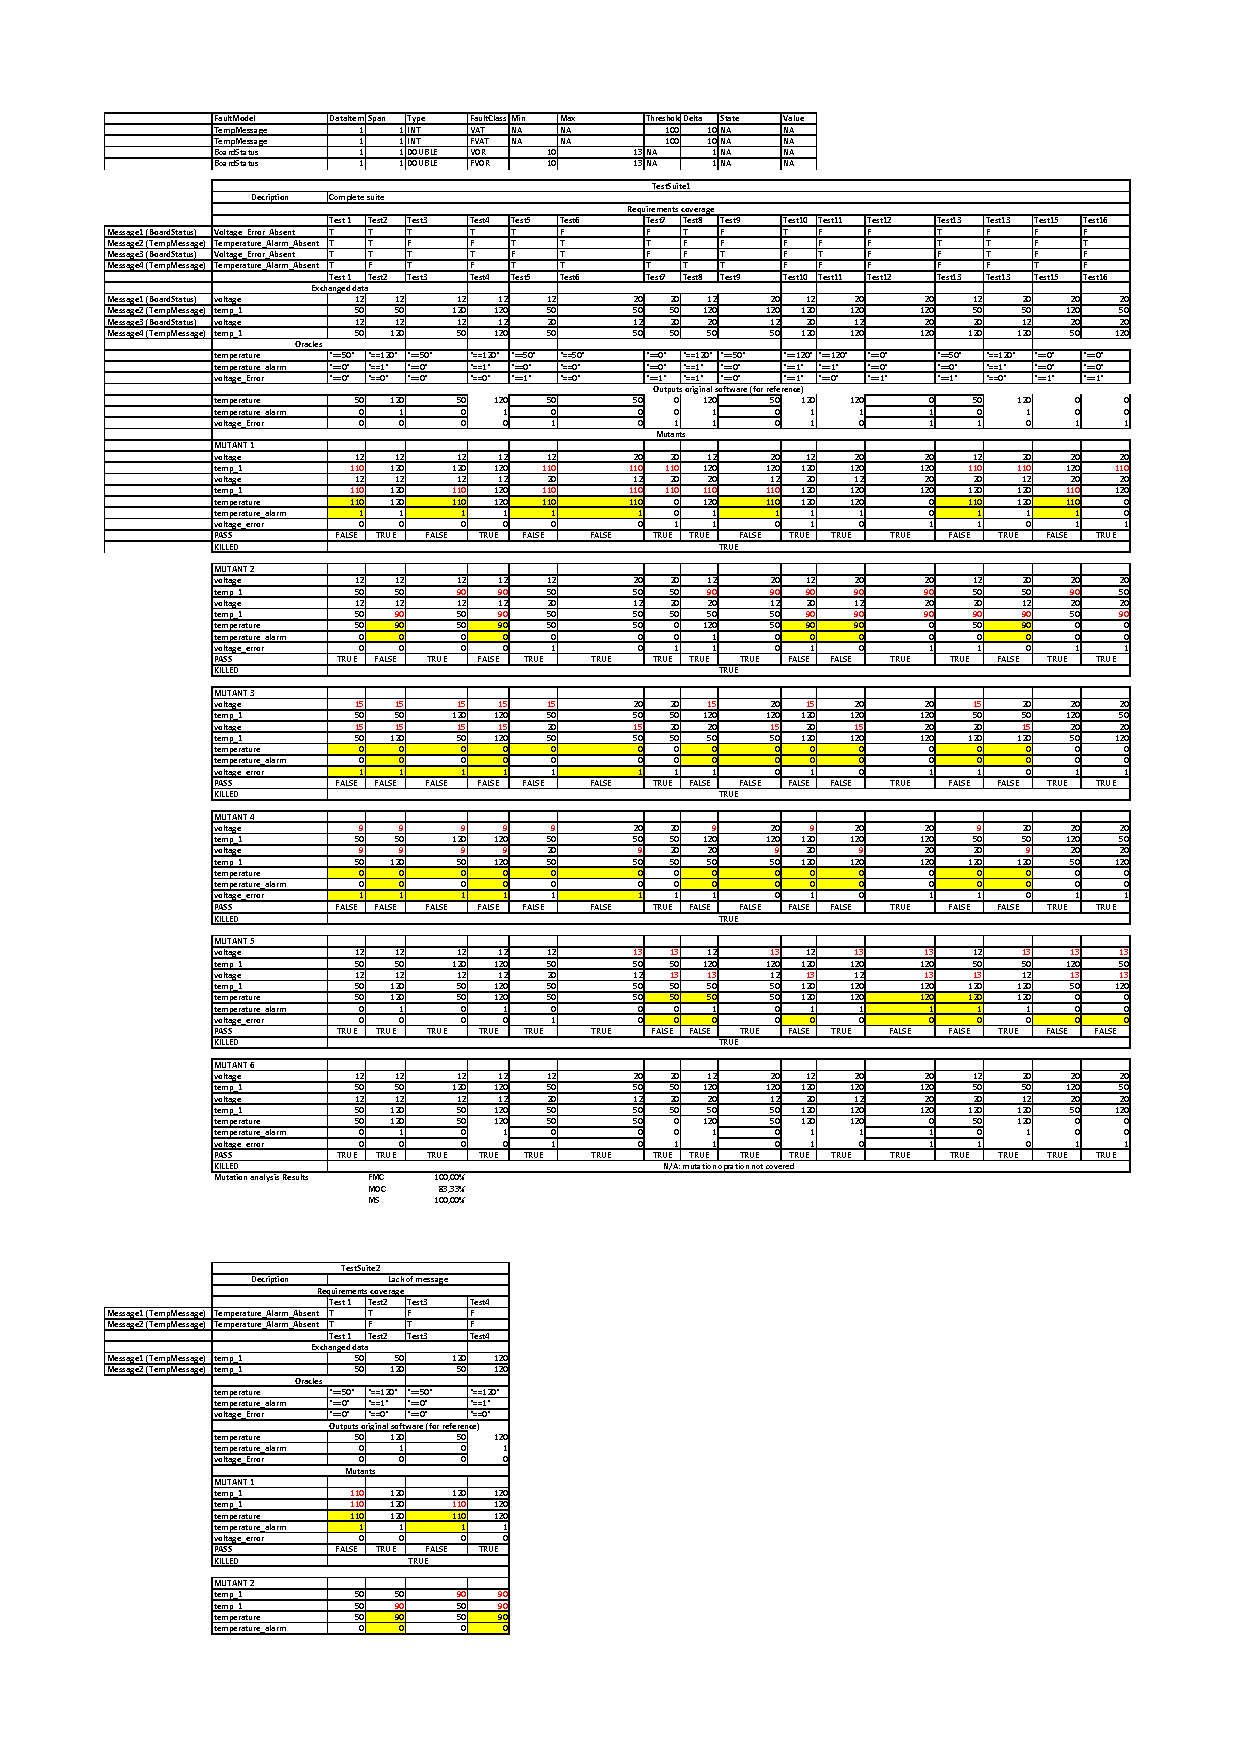
\includegraphics[width=18cm]{damat/DataDrivenExample3A}
\caption{Running example set 3 - Part A.}
\label{fig:damat:RunningExample3A}
\end{figure}

\begin{figure}[tb]
\centering
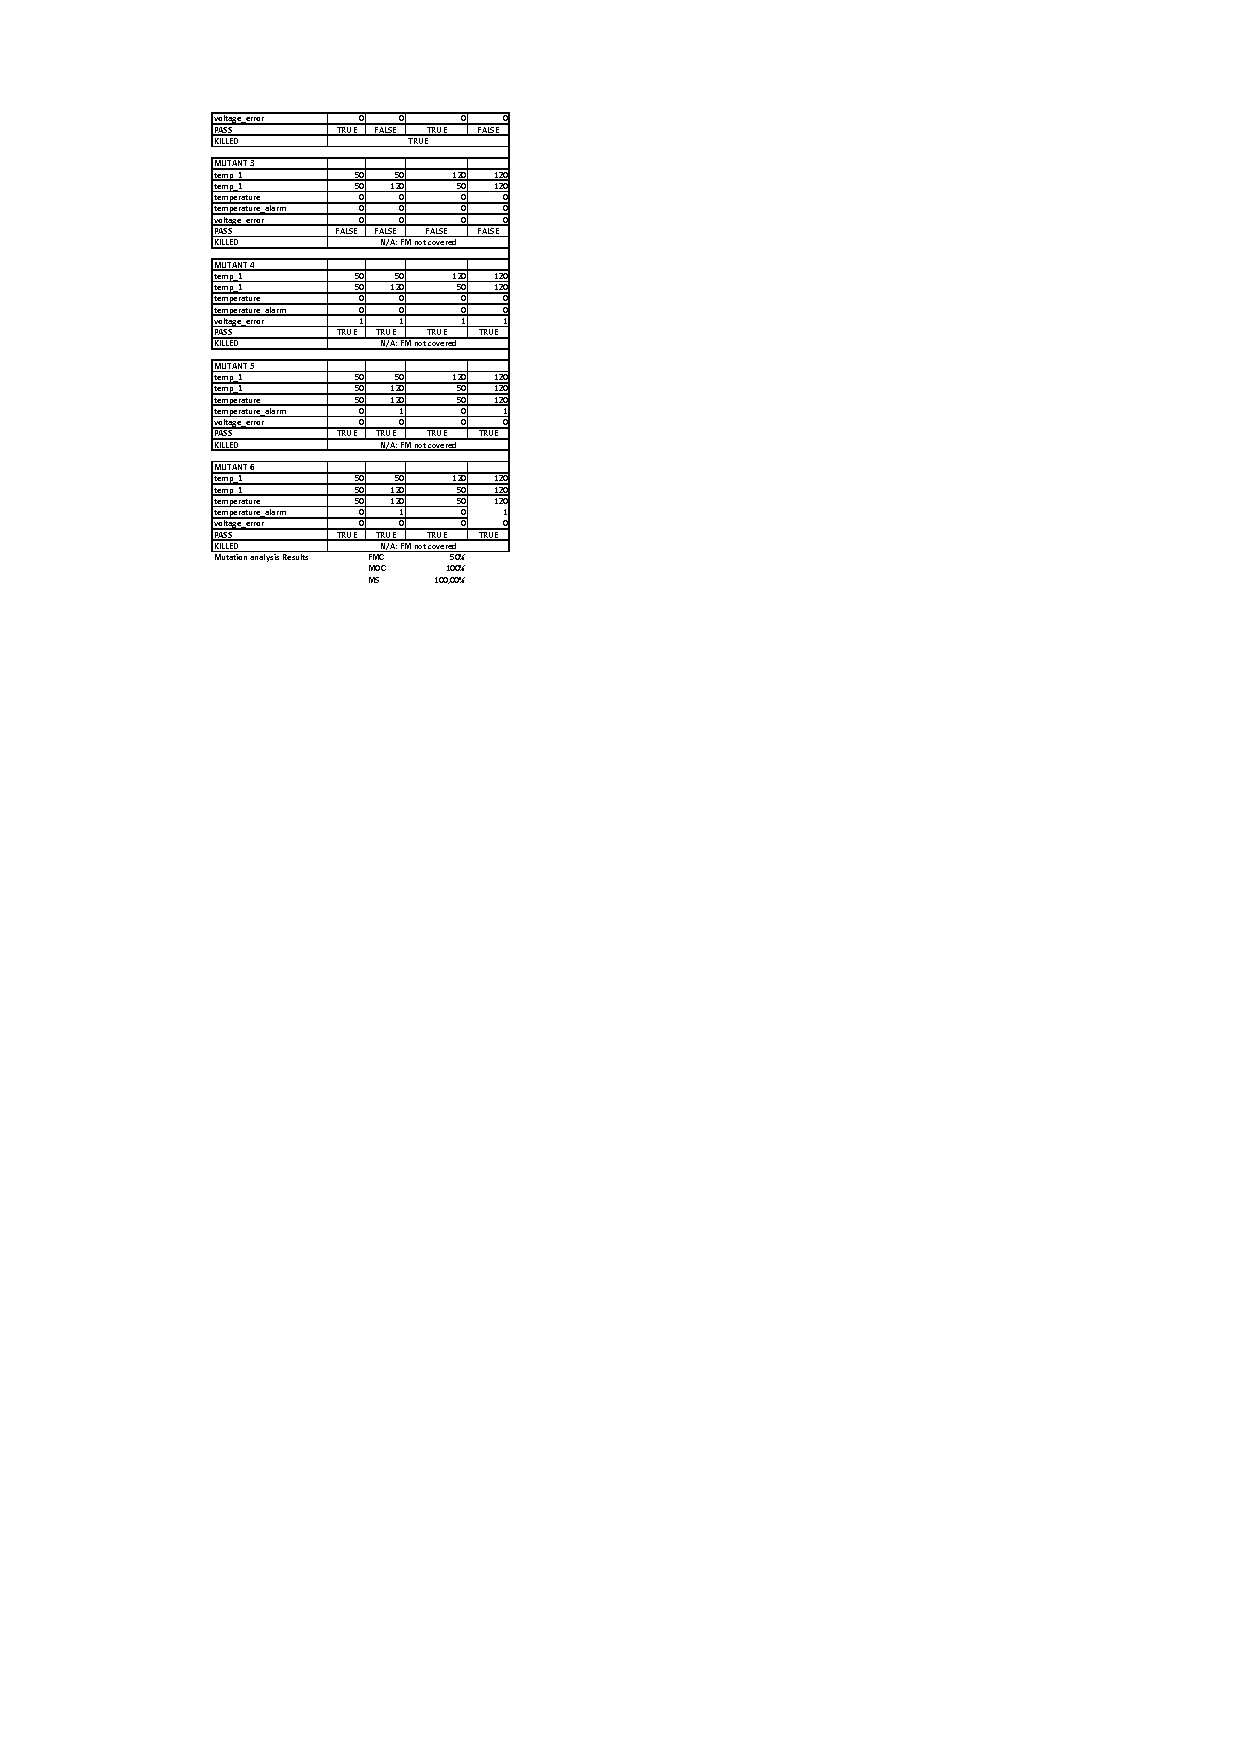
\includegraphics[width=18cm]{damat/DataDrivenExample3B}
\caption{Running example set 3 - Part B.}
\label{fig:damat:RunningExample3B}
\end{figure}


\paragraph{TestSuite2}



\begin{figure}[tb]
\centering
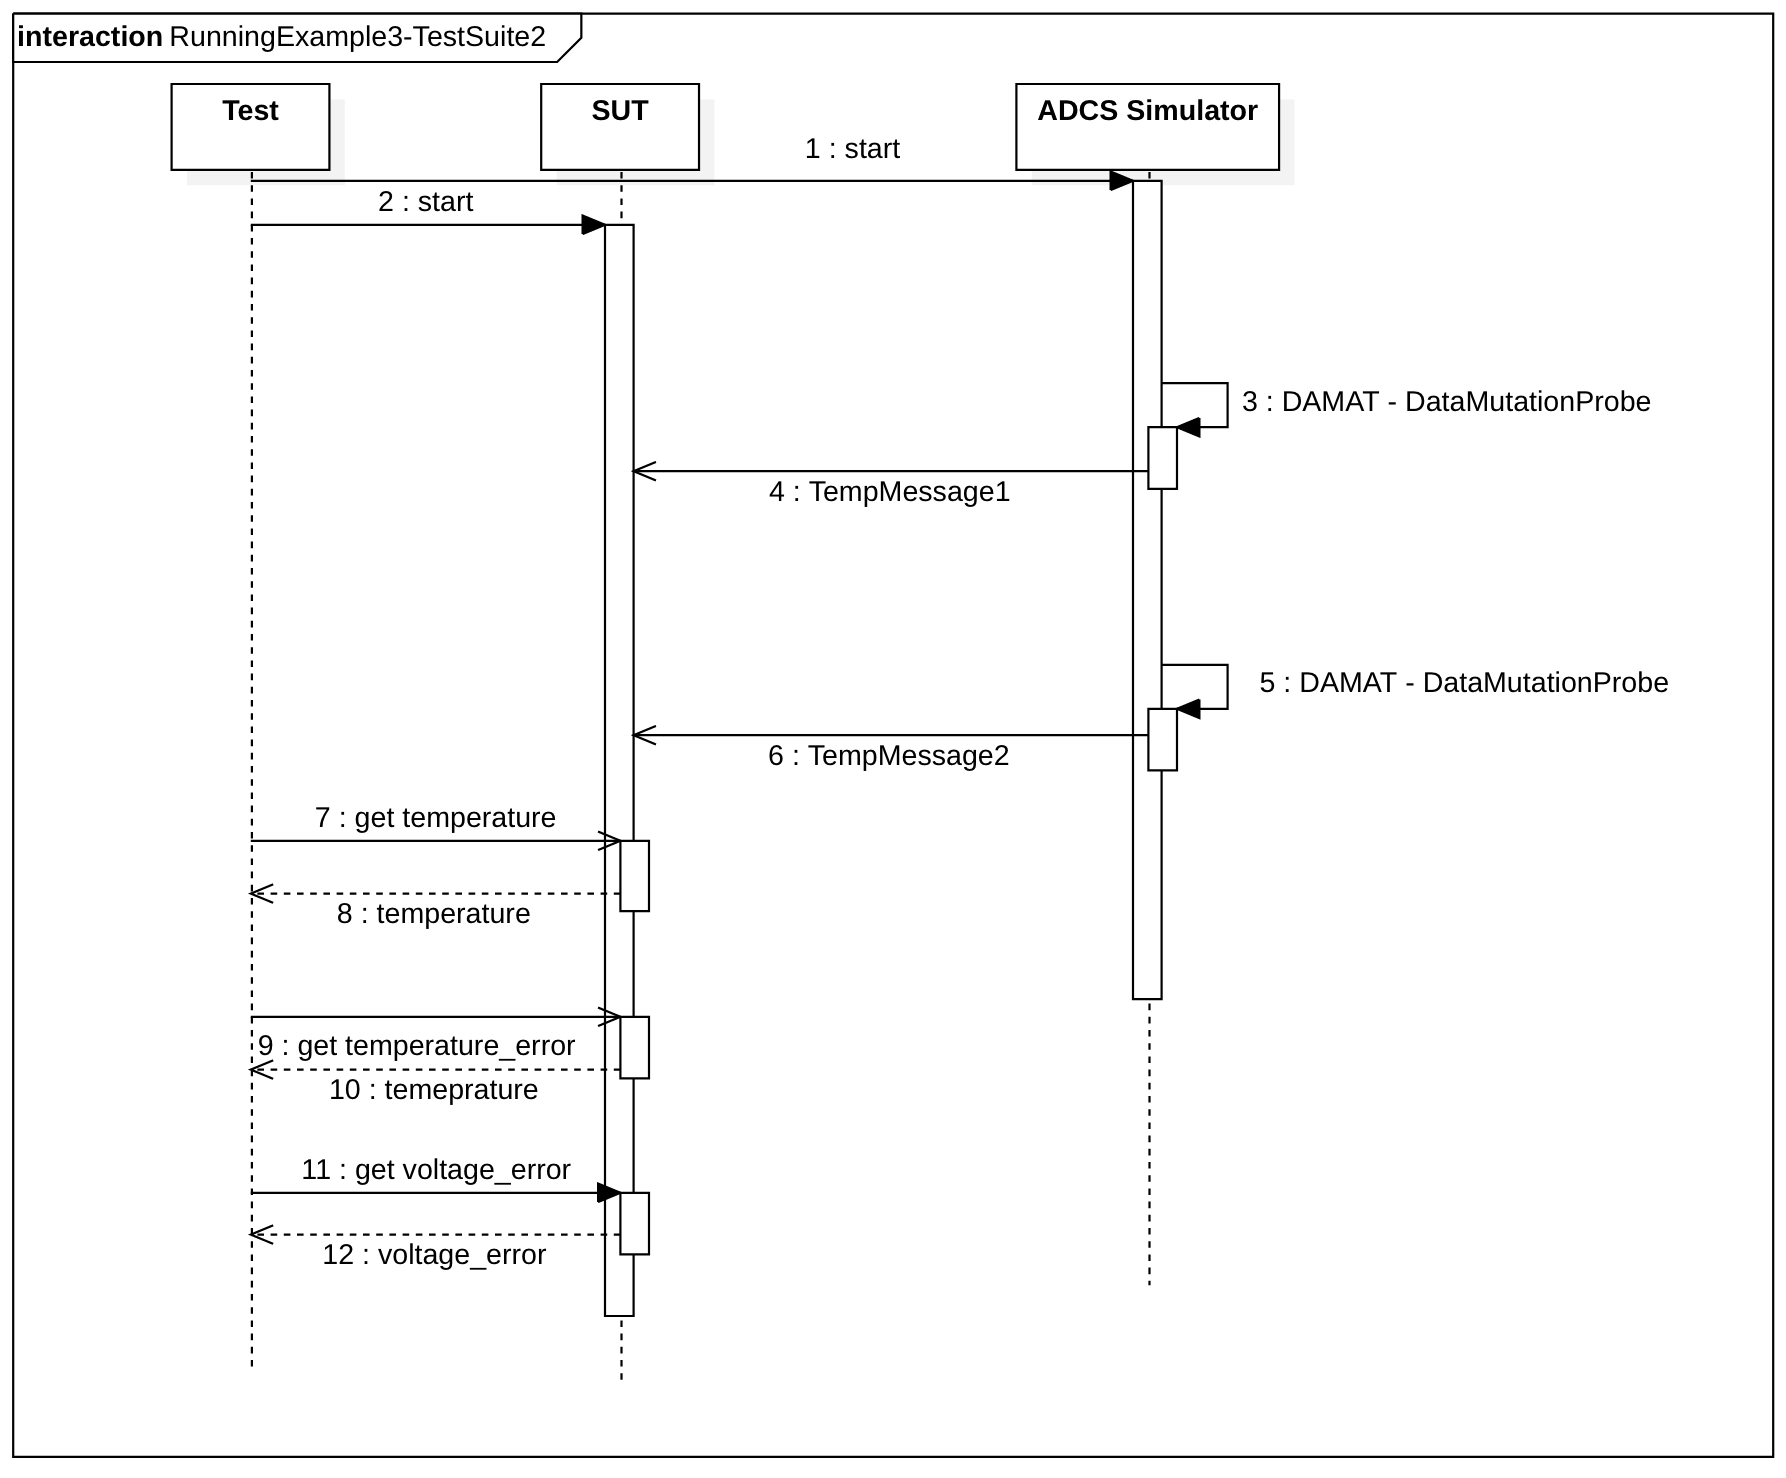
\includegraphics[width=8cm]{damat/images/runningExamplesSequence3_2.png}
\caption{Interactions exercised by the test cases of TestSuite2 in the running example set 3.}
\label{fig:damat:RunningExample3Sequence2}
\end{figure}

TestSuite 2 does not trigger messages of type BoardStatus; its interactions are depicted in Figure~\ref{fig:damat:RunningExample3Sequence2}. For the remaining message type (i.e., TempMessage) it covers all the possible combinations of temperature alarms being present/absent for two TempMessages sent in sequence; in total, we have 4 test cases.

The fault model BoardStatus is not covered; therefore the fault model coverage (FMC) is 50\%. Since MUTANTS 3 to 6 belong to BoardStatus they are not considered in the computation of the other mutation analysis metrics. MOC and MS are thus 100\%; indeed all the mutants not belonging to BoardStatus are killed by the test suite.

MUTANT 1 could be live only if relevant oracles are missing; more precisely, only if oracles concerning the nominal temperature value are missing. MUTANT 1 is killed by TestSuite2.

MUTANT 2 could be live only if relevant oracles are missing; indeed, only if oracles concerning the non nominal temperature value are missing. MUTANT 2 is killed by TestSuite2.
% !TEX root = MAIN.tex




\section{Data-driven Mutation Testing: DAMTE} % (fold)
\label{sec:data:test_suite_augmentation}



The \INDEX{test suite augmentation process} it consists of four activities \INDEX{Identify Test Inputs}, \INDEX{Generate Test Oracles}, \INDEX{Execute the SUT}, \INDEX{Fix the SUT}. It has the objective of increasing the score generated by the mutation analysis process.

FAQAS focussed on a methodology (i.e., data-driven mutation testing, \INDEX{DAMTE}) that specifies how to rely on KLEE to generate test inputs that increase the fault model coverage and the mutation operation coverage.
FAQAS does not address increasing the mutation score because infeasible in automated manner.
We recall that two might be the reasons for a low MS: poor oracle quality and missing test input sequences.
If the low mutation score is due to poor oracle quality, manual work is needed because automated approaches to automatically generate test oracles in the presence of system or integration test suites are not available. 
If the low mutation score is due to missing test input sequences (i.e., the software does not reach the state in which it could kill the mutant), manual work is required because existing test generation approaches (e.g., KLEE) might suffer from scalability problem that prevent bringing the system into a desired state; also, they cannot deal with systems whose components communicate through channels. 

For the cases targeted by FAQAS (i.e.,
in the presence of fault model coverage and mutation operation coverage below 100\%), test generation has the objective of generating test inputs that enable the application of all the mutation operators. 
We thus rely on an  \INDEX{extended data mutation probe} that
invokes a version of the data mutation API that instead of mutating the data targeted by the mutation operator not covered by the fault model, includes a reachability assertion that is used to make KLEE find a test input that reaches the mutant code. The test input shall then be inspected by the engineer, who will need then to integrate it into his test suite.
%Figure~\ref{fig:dataDrivenTestSuiteAugmentationB} exemplifies how data driven mutation testing works, for the producer consumer and client-server cases.
%
%
%
%
%\begin{figure}[h]
%  \centering
%    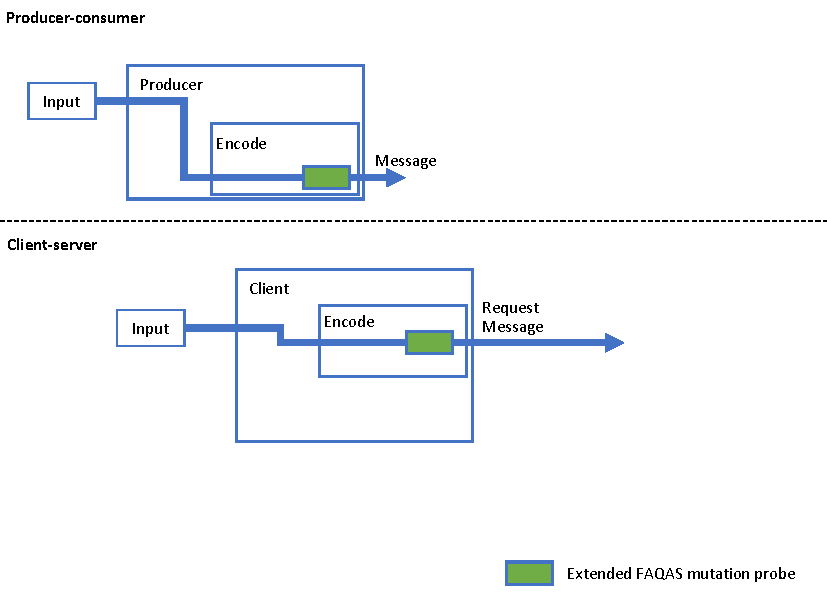
\includegraphics[width=14cm]{images/dataDrivenTestSuiteAugmentationB}
%      \caption{Data-driven mutation analysis for different architectures.}
%      \label{fig:dataDrivenTestSuiteAugmentationB}
%\end{figure}










%% !TEX root = MAIN.tex

\chapter{Data-driven Mutation Testing}
\label{chapter:datamutation}

% !TEX root = MutationTestingSurvey.tex

\section{Overview of the Data-driven Mutation Testing Process}
\label{sec:dataProcess}

	\begin{figure}
	\centering
		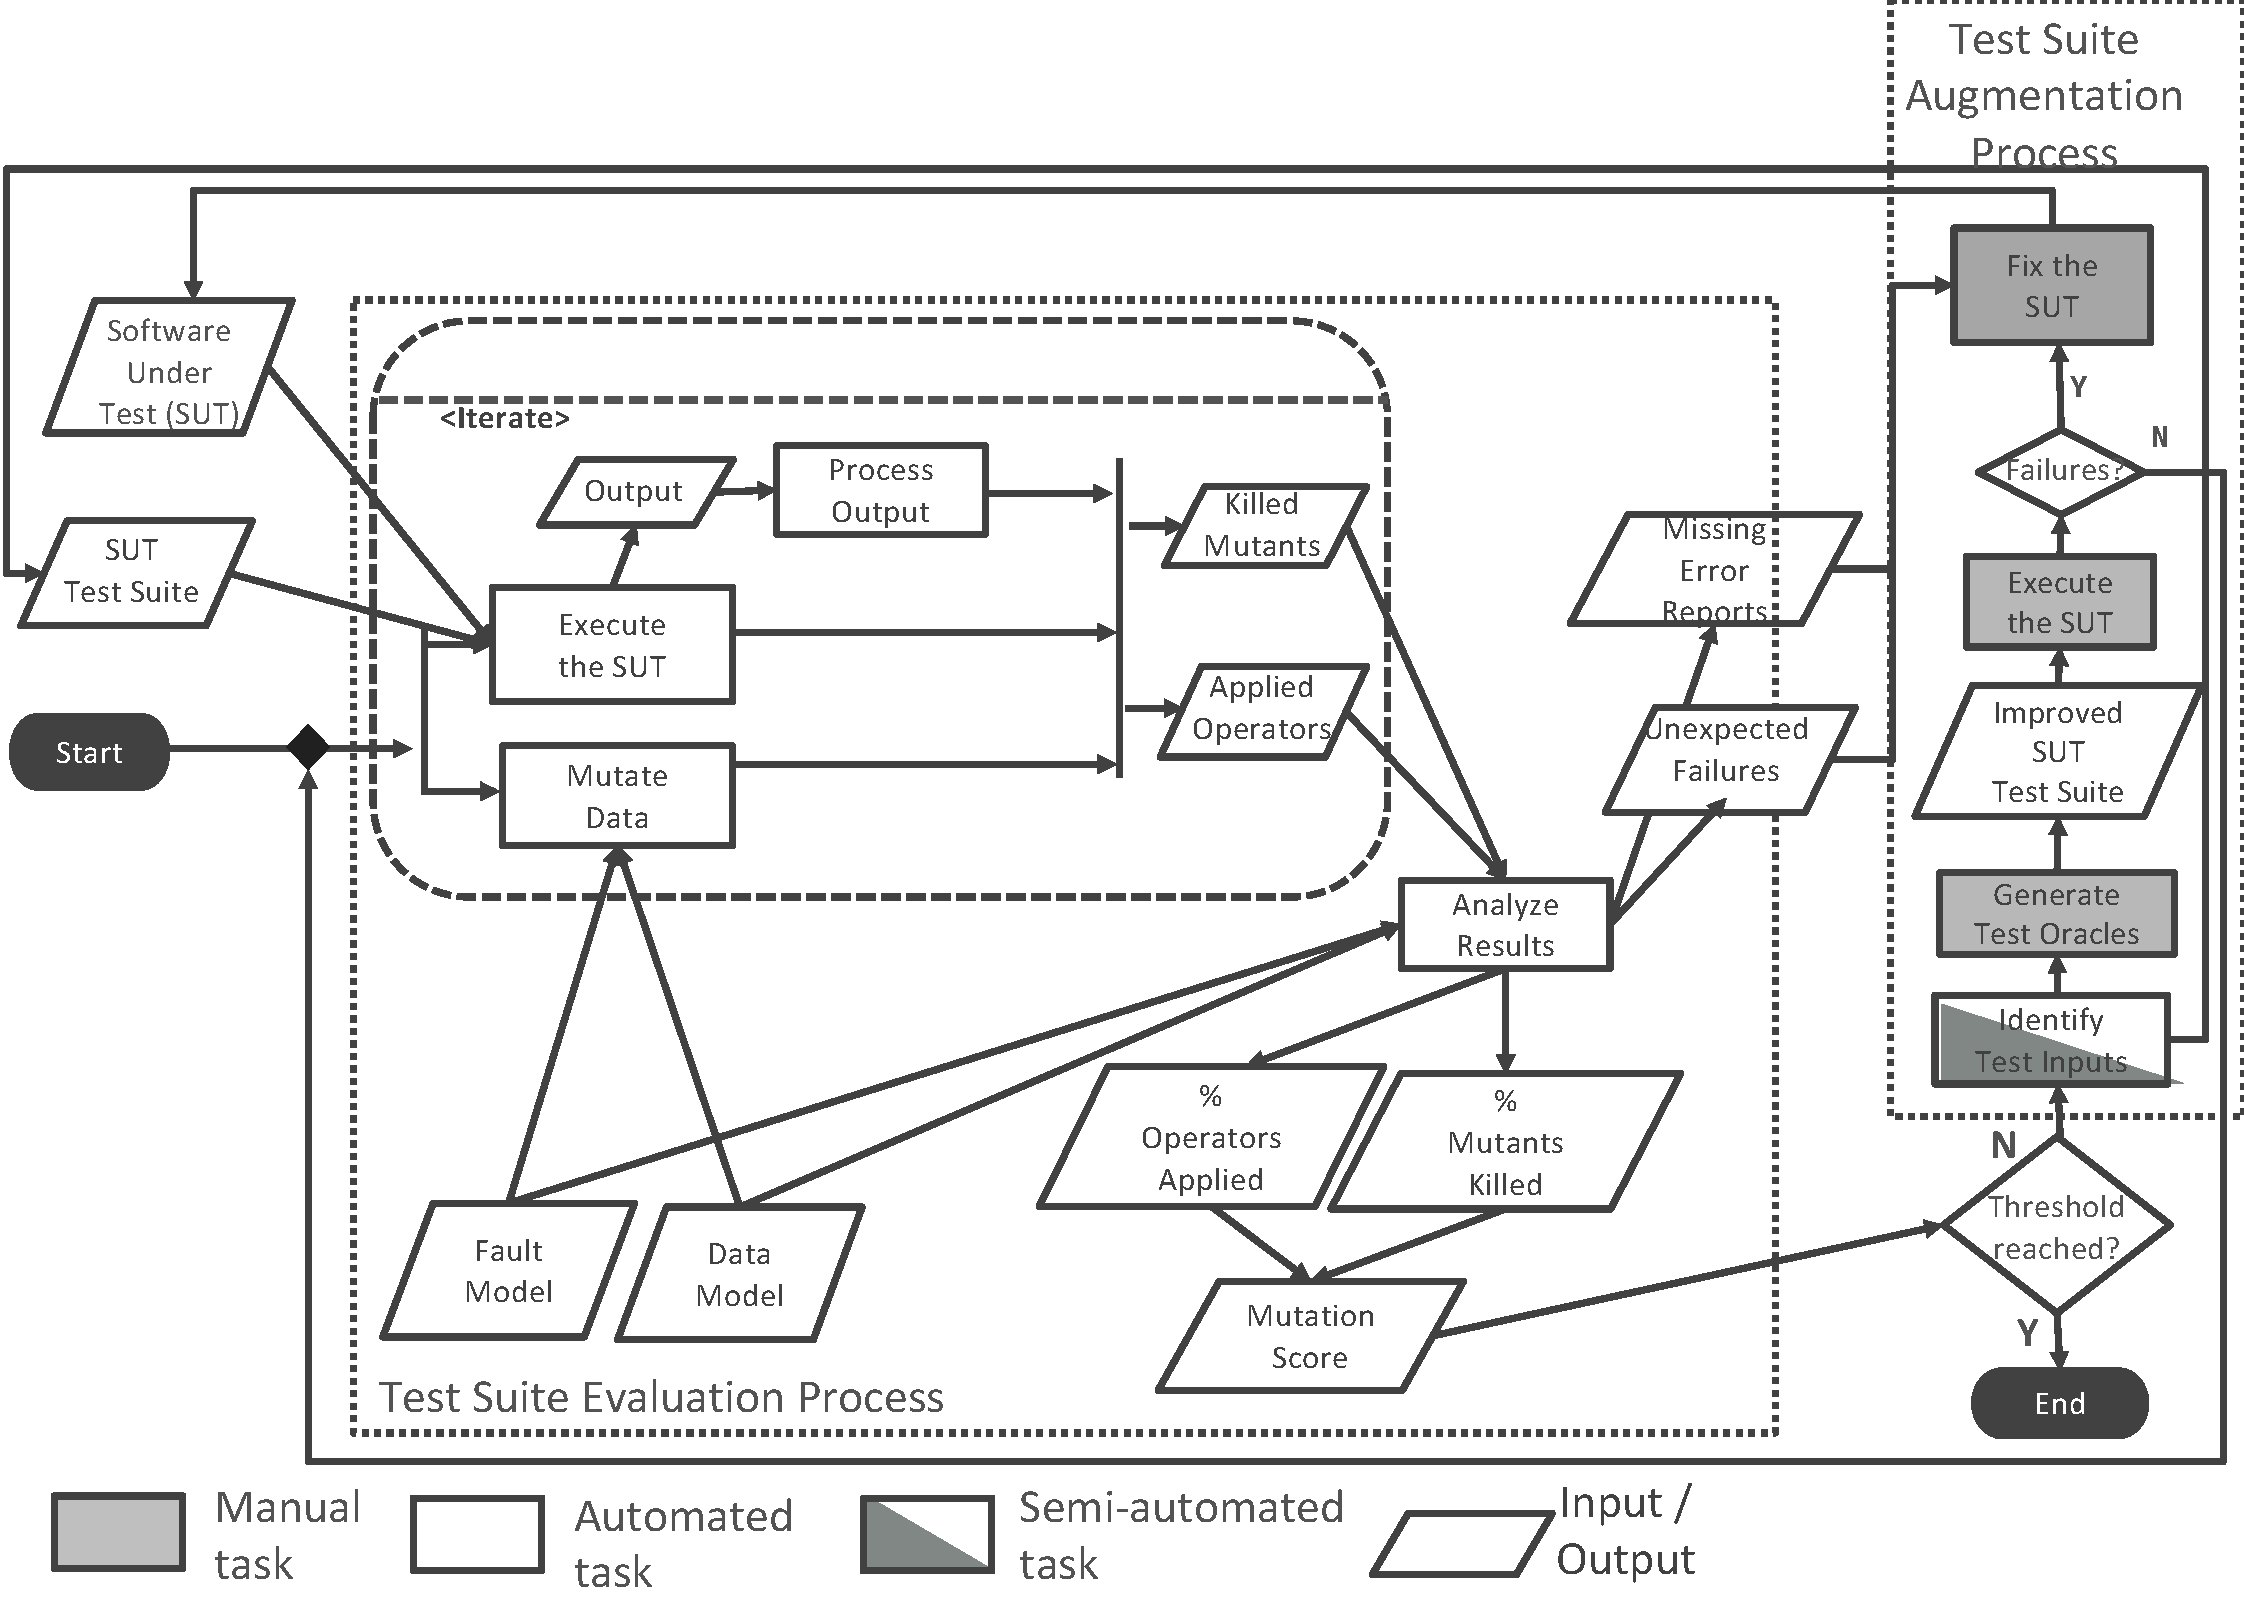
\includegraphics[width=\textwidth]{images/dataProcess}
		\caption{Data-driven Mutation Testing Process.}
		\label{fig:data:process}
	\end{figure}



This Chapter defines a test suite assessment process based on the injection of faults in the data processed by software components; we refer to this process as \INDEX{data-driven mutation testing}. 
%The definition of data-driven mutation testing is a unique contribution of this book; it has not been presented in previous literature work.

Data-driven mutation testing aims to assess test suites by simulating faults that affect the data produced, received, or exchanged by the software and its components.
It is based on a \INDEX{fault model} capturing the type of data faults that might affect the system. The fault model is produced by software engineers based on their domain knowledge and experience~\cite{di2015generating}. \MREVISION{C18}{The considered faults might be due to programming errors, hardware problems, or critical situations in the environment (e.g., noise in the channel).} The data is then automatically  mutated (i.e., modified) by a set of operators that aim to replicate the faults in the fault model. For example, the \INDEX{bit flip operator} flips a randomly selected bit of a field of the transmitted data (see Section~\ref{sec:faultModel}). 
%Mutation operators can be applied multiple times, on different data chunks or over repeated executions of a test case, ti


Figure \ref{fig:data:process} shows the reference data-driven mutation testing process that will be considered in FAQAS. The process is based on two main sub-processes, \EMPH{test suite evaluation} and \EMPH{test suite augmentation}, which are described in Sections~\ref{sec:data:test_suite_evaluation}~and~\ref{sec:data:test_suite_augmentation}, respectively. Differently from the code-driven mutation testing process introduced in Section~\ref{sec:process}, the data-driven mutation testing process has not been formalized by existing software testing literature. An extensive discussion of related work has been presented in deliverable D1.

Since data-driven mutation testing alters the data produced, received, or exchanged by the software or its components, it should be applied to evaluate test suites that trigger the execution and communication between multiple components (e.g., system or integration test cases). Data-driven mutation testing is not meant to be applied to assess unit test suites.

\clearpage
\section{Test Suite Evaluation} % (fold)
\label{sec:data:test_suite_evaluation}

The test suite evaluation process consists of three activities \EMPH{Execute the SUT}, \EMPH{Mutate Data},  and \EMPH{Analyze Results}.
The activity \INDEX{Execute the SUT} indicates that the SUT is executed against its automated test suite. 
The activity \INDEX{Mutate Data} concerns the automated modification of either the data received by the software, the data produced by the software, or the data exchanged by software components.
In Figure~\ref{fig:data:process}, the activity \EMPH{Mutate Data} is executed in parallel to the activity \EMPH{Execute the SUT} since data modification should occur at runtime during test cases execution, to simulate software faults affecting the data processed by the software.



%The fault model enables engineers to minimize the presence of equivalent mutants.
%The data model may capture the relation between inputs and outputs of the system

\begin{figure}
	\centering
		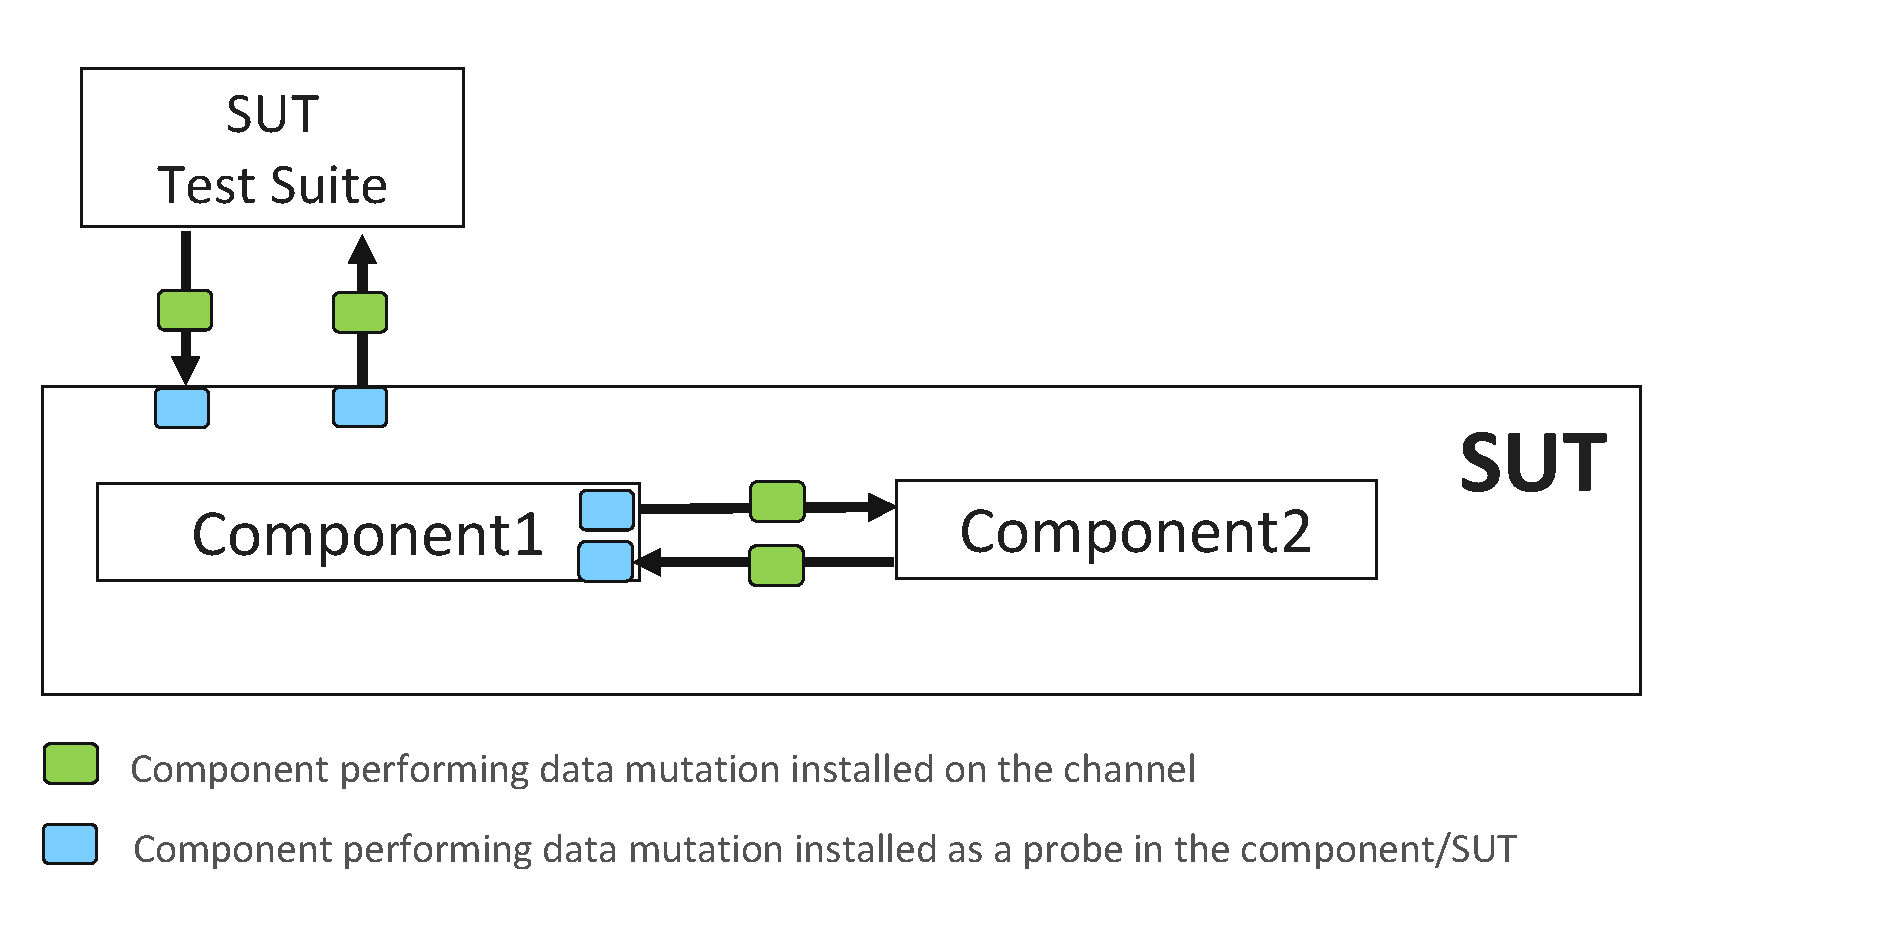
\includegraphics[width=10cm]{images/dataMutationExample}
		\caption{Example of implementation of a data mutation solution.}
		\label{fig:data:mutateData}
	\end{figure}
	
Figure~\ref{fig:data:mutateData} provides an example of how the Mutate Data activity can be implemented. Figure~\ref{fig:data:mutateData} shows that, to implement data mutation, it is necessary to integrate additional components that alter the data exchanged by the SUT components at runtime on a certain communication layer. We call such components \INDEX{mutation probes}.

An ideal target for data-driven mutation testing is the communication between loosely coupled software components; typically the ones that run on separated pieces of hardware (e.g., the on board controller and the ADCS).
In FAQAS case studies, the communication between such software components is performed by relying on APIs of a dedicated communication layer; which is typical in well designed software systems. The main functionality of such communication layer is to serialize and deserialize data that should be transmitted on the communication channel. In FAQAS case studies, the communication layer is either implemented in-house by the company that produced the case study or it is built by relying on the ASN.1 compiler architecture. In both the two cases, the communication layer implements distinct functions to serialize and deserialize data.
For this reason, in FAQAS, we expect mutation probes to be \EMPH{integrated into the software API functions that either serialize or deserialize the data being sent on the communication channel}.

In the case of a communication layer implemented in-house, we expect mutation probes to be integrated into the software under test by engineers who \EMPH{manually} add calls to the functions of a \INDEX{data-driven mutation testing API} in the source code of the software. Indeed, since communication APIs vary from system to system, it is not possible to define a tool that automatically modifies the source code or the executable code of the SUT.  Instead, we provide a \INDEX{data-driven mutation testing API} that implements the logic for mutating the data specified by the engineer.
To be applicable to a wide rande of software systems, the API will provide methods that enable mutating data buffers provided as C arrays.
Figure~\ref{fig:data:mutationProbes} shows an example of a mutation probe manually integrated into the source code (API method names begin with the prefix \emph{\_FAQAS}).

In the case of a communication layer implemented by relying on the ASN.1 compiler, the FAQAS framework will automatically introduce mutation probes into the code that deserialize data.




\begin{figure}
	\centering
		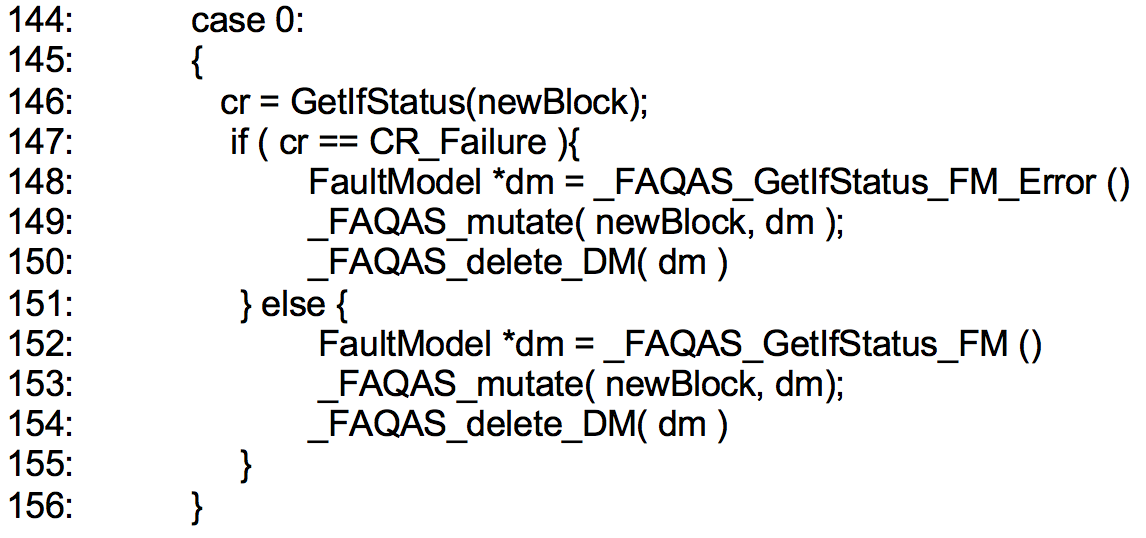
\includegraphics[width=10cm]{images/dataMutationProbes}
		\caption{Example of integration of data mutation probes.}
		\label{fig:data:mutationProbes}
	\end{figure}

%\TODO{ADD concrete example of integration}

	
%Data-driven mutation testing is driven by a faulty model specifying how to alter the data (i.e., the attributes declared in an ASN.1 grammar or the array items).	
In deliverable D1, we have clarified that, in a generic data-driven mutation testing process, the activity \EMPH{Mutate Data} may require a \INDEX{data model} that captures the characteristics and structure of the data to be mutated. 
The data model should be used to load a stream of bytes in structured form (e.g., an instance of a given data structure), which is necessary to drive data mutation. 
Also, the activity \EMPH{Mutate Data} should be driven by a \INDEX{fault model} that specifies the set of mutation operators to apply~\cite{di2015generating}. 
In FAQAS, the data model and the fault model are coupled into a same structured representation, i.e., the \INDEX{FAQAS fault model}, which is presented in Section~\ref{sec:faultModel}.


The activities \EMPH{Execute the SUT} and \EMPH{Mutate Data} are repeated till all the faults of the fault model had been applied. The possible stopping criteria are described in Section~\ref{sec:mutantsExecution}. 

The activity \INDEX{Process Outputs} processes all the outputs generated during the execution of test cases.
The collected outputs include the result of test cases execution (i.e., the list of test cases that either passed or failed) and the logs generated by the SUT during testing.
In the context of data-driven mutation testing both the \INDEX{test results} and the \INDEX{log files} are necessary to determine if a test suite kills a mutant.
Indeed, \emph{in the context of data-driven mutation testing a mutant is killed either if a test case fails, or if the software activates robustness features capable of handling the specific data fault.}
We need log files to determine if robustness features had been triggered.
For example, a system that implements a \INDEX{robust communication protocol} might simply request again the packets affected by errors thus avoiding failures. In this case, we need to inspect the log files to determine if the robustness feature had been triggered.
The fault model is expected to include only data fault classes that should either lead to failures or make the system generate an error entry in the log file.

Differently from code-driven mutation testing, data-driven mutation testing does not alter the software implementation but only the data processed by software components, for this reason it may help engineers to \INDEX{identify existing faults}, an objective that cannot be achieved by code-driven mutation testing. 
This is the case when \emph{Missing Error Reports} or \emph{Unexpected Failures }(e.g, crashes) are observed. In both the two cases, engineers should fix the system. In code-driven mutation testing, faults can be detected only after introducing new test cases that kill the generated mutants.

The activity \INDEX{Analyze Results} provides an assessment of the quality of the test suite for the SUT.
It is driven by two objectives:
\begin{itemize}
\item[(O1)] determine if the test suite is capable of detecting software faults that affect the data processed by the software components 
(e.g., we expect a test suite to fail in case the data exchanged by two components contains invalid values).
\item[(O2)] determine if the test suite exercises enough software behaviours to discover all the possible faults that may affect the data produced by the system
(i.e., it should be possible to alter the processed data to generate faulty data according to the fault model). 
\end{itemize}

\MREVISION{C19}{Objectives O1 and O2 are complementary, \REVTWO{C33}{they both should be addressed by data mutation.}
For example, a use case scenario for data-driven mutation testing could be the following: (i) data-driven mutation testing is applied to the data exchanged by \emph{component 1} and \emph{component 2} in Figure~\ref{fig:data:mutateData}, (ii) the data exchanged by the two components follow the data model in Figure~\ref{fig:DataDrivenSimpleExample}, and (iii) mutation testing is performed by applying the bit-flip mutation operator to every field of the messages being exchanged.
The data model in Figure~\ref{fig:DataDrivenSimpleExample} consists of a UML class diagram that indicates that the two components can send messages whose type can be either \emph{TimeMessage} or \emph{DataMessage}. A \emph{TimeMessage} contains only one field of type Long, which is the timestamp. 
A \emph{DataMessage} contains two fields, one field of type \emph{Integer} capturing the size of the payload, and one array of bytes containing the payload. 
Objective O1 is fulfilled when every mutant leads to the failure of least one test case.
Objective O2 is fulfilled when mutation testing generates at least (i) one \emph{TimeMessage} with field \emph{timestamp} being altered,
(ii) one \emph{DataMessage} with field \emph{size} being altered,
and (iii) one \emph{DataMessage} with field \emph{payload} being altered.
For a test suite consisting of two test cases that trigger the exchange of the messages as in the bottom-left part of Figure~\ref{fig:DataDrivenSimpleExample}, the execution of the bit flip mutation operator may lead to messages that lead to test failures. Since all the mutants are killed (i.e., the two test cases fail), objective O1 is achieved. However, the test suite does not lead to the exchange of any message of type \emph{DataMessage}, for this reason objective O2 is not achieved. Objective O2 enables us to determine that the test suite does not excercise the case in which the two components exchange messages of type \emph{DataMessage}. When data-driven mutation testing is performed against components that are expected to guarantee robustness against the exchange of erroneous data, as a by-product, objective O2 also ensures that components' robustness is properly tested.}



\REVTWO{C34}{Activity \emph{Analyze Results} concerns the automated computation of the \INDEX{mutation score} from execution data. It is 
computed as the weighted average of the percentage of mutants being killed and the percentage of mutation operators applied.}
The former enables data-driven mutation to achieve objective O1 in Section~\ref{sec:dataProcess}, the latter objective O2. 
%Details are provided in Section~\ref{sec:data:mutationscore}.

\REVTWO{C34}{Activity \emph{Analyze Results} takes as input the the data model, the fault model, the list of killed mutants, and the list of mutation operators applied.}
The list of applied mutation operators should enable engineers to determine if all the available mutation operators have been applied.


\begin{figure}[t!]
  \centering
    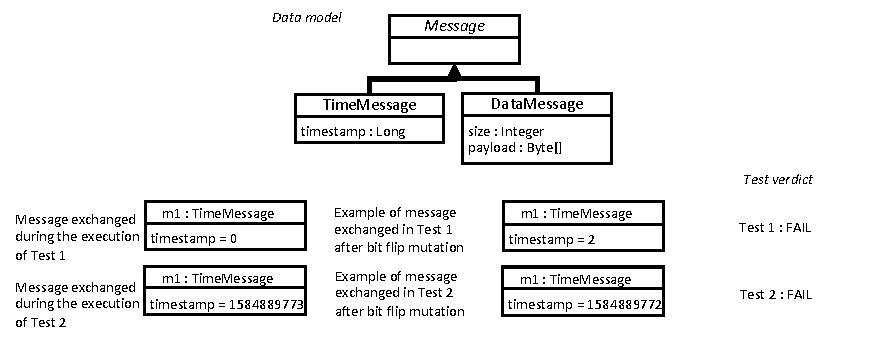
\includegraphics{images/DataDrivenSimpleExample}
      \caption{Simplified data mutation example.}
      \label{fig:DataDrivenSimpleExample}
\end{figure}

\clearpage



\clearpage
\subsection{FAQAS Fault Model}
\label{sec:dataModel}
\label{sec:faultModel}





A building block of the fault model are a set of \EMPH{data fault classes}.
A  \INDEX{data fault class} captures the type of an error that might affect the data. In turns, it specifies the mutation that should be applied in order to replace valid data with erroneous data. For each fault class we have defined a corresponding \INDEX{data mutation operator} having the same name. 
Each {data mutation operator} performs data mutation by applying a \INDEX{data mutation operation} (e.g., set a value above the upper range value). Mutation operators might apply one or more data mutation operations.
Each data mutation operator can be configured with a set of parameters. 

Table~\ref{table:faultModel:FAQAS} provides the list of data fault classes supported by FAQAS along with a description. For each fault class we indicate the data types to which it is expected to be applied, we identify four data types: 
\begin{itemize}
\item int, which indicates an integer
\item float, which indicates a floating point number
\item double, which indicates a double precision floating point number
\item bin, which indicate data that should be treated in its binary form
\end{itemize}


In FAQAS, data-driven mutation testing is performed by modifying either data that is stored in an array or in a data structure defined through the ASN.1 grammar. The following subsections describe the two distinct cases.







% !TEX root = ../MAIN.tex
\begin{table}[h]
\begin{center}
\scriptsize
\begin{tabular}{|p{2cm}|p{2cm}|p{4cm}|p{6cm}|}
\hline
\textbf{Fault Class}&\textbf{Types}&\textbf{Parameters}&\textbf{Description}\\
\hline
Value above threshold (VAT)&
\begin{minipage}{6cm}
INT\\
LONG INT\\
FLOAT\\
DOUBLE
\end{minipage}
&
\begin{minipage}{6cm}
T: threshold\\
D: delta with respect to threshold\\
\end{minipage}
&
\begin{minipage}{6cm}
The value is above a threshold T for a delta D. 

\EMPH{Data mutation operation:} The mutation is performed by replacing the current value (a number) with a value of the same type that is equal to $(T+D)$.
\end{minipage}
\\

\hline
Value below threshold (VBT)&
\begin{minipage}{6cm}
INT\\
LONG INT\\
FLOAT\\
DOUBLE
\end{minipage}
&
\begin{minipage}{6cm}
T: threshold\\
D: delta with respect to threshold\\
\end{minipage}
&
\begin{minipage}{6cm}
The value is below a threshold T for a delta D. 

\EMPH{Data mutation operation:} The mutation is performed by replacing the current value (a number) with a value of the same type that is equal to $(T-D)$.
\end{minipage}
\\



\hline
Value out of range (VOR)&
\begin{minipage}{4cm}
INT\\
LONG INT\\
FLOAT\\
DOUBLE
\end{minipage}
&
\begin{minipage}{4cm}
MIN: minimum valid value\\
MAX: maximum valid value\\
D: delta with respect to minimum/maximum valid value
\end{minipage}
&
\begin{minipage}{6cm}
The value is out of the valid range MIN-MAX. 

\EMPH{Data mutation operations (2):}  The mutation is performed by replacing the current value (a number) with 
\begin{itemize}
\item a value of the same type that is equal to $(MIN-D)$
\item a value of the same type that is equal to $(MAX+D)$
\end{itemize}
\end{minipage}
\\

\hline
Bit flip (BF)&
BIN
&
\begin{minipage}{4cm}
MIN: lower bit\\
MAX: higher bit\\
STATE: mutate only if the bit is in the given state\\
\TRFOUR{VALUE: integer specifying the number of bits to mutate}\\
\end{minipage}
&
\begin{minipage}{6cm}
A number of bits randomly chosen in the positions between MIN and MAX (included) are flipped.

\EMPH{Data mutation operation:} the operator flips N randomly selected bit.
If STATE is specified, the mutation is applied only if  the bit is in the specified state. Parameter VALUE specifies the number of bits to mutate.
\end{minipage}
\\

\hline
Invalid numeric value (INV)&
\begin{minipage}{6cm}
INT\\
LONG INT\\
FLOAT\\
DOUBLE
\end{minipage}
&
\begin{minipage}{4cm}
MIN: lower valid value\\
MAX: higher valid value\\
\TRFOUR{D: distribution to follow}\\
\TRFOUR{VALUE: mean value for normal distribution}\\
\end{minipage}
&
\begin{minipage}{6cm}
The value is legal (i.e., in the specified range) but different than the current one, which, in this case, is expected to be consistent with the status of the system.

\EMPH{Data mutation operation:} Mutation is performed by replacing the current value with a different value randomly sampled in the specified range. The parameter D specified the distribution to follow when performing the mutation\footnote{In our implementation 0 indicates uniform, 1 indicates normal around the specified value (but in range).}
\end{minipage}
\\

\hline
Illegal Value (IV)
&
\begin{minipage}{6cm}
INT\\
LONG INT\\
FLOAT\\
DOUBLE
\end{minipage}
&
\begin{minipage}{6cm}
VALUE: illegal value that is observed\\
\end{minipage}
&
\begin{minipage}{6cm}
The value is illegal and equal to the provided one (i.e., parameter \emph{VALUE}).

\EMPH{Data mutation operation:} Mutation is performed by replacing the current value with the value \emph{VALUE}, if different than the current one.
\end{minipage}
\\

\hline
\TRFOUR{Anomalous Signal Amplitude (ASA)}
&
\begin{minipage}{6cm}
INT\\
LONG INT\\
FLOAT\\
DOUBLE
\end{minipage}
&
\begin{minipage}{6cm}
T: change point\\
D: delta to add/remove\\
V: value to multiply\\
\end{minipage}
&
\begin{minipage}{6cm}
The value is modified by amplifying/reducing it by a factor V and adding or removing D from the observed value. It is used to "amplify" a signal in a constant manner to simulate unusual signal. T indicates the observed value below which instead of adding  we subtract .

\EMPH{Data mutation operation:} Mutation is performed by replacing the current value ($v$) with the value ($v'$) computed as follows:

\[
v' =  
    \begin{cases}
      T+(  (v-T)*V  ) + D   & \mathit{if}\ v \ge T\\
      T - (  (T-v)*V  ) - D   & \mathit{if}\ v < T
    \end{cases}       
\]
\end{minipage}
\\


\hline
\TRFOUR{Signal Shift (SS)}
&
\begin{minipage}{6cm}
INT\\
LONG INT\\
FLOAT\\
DOUBLE
\end{minipage}
&
\begin{minipage}{6cm}
D: delta by which the signal should be shifted\\
\end{minipage}
&
\begin{minipage}{6cm}
The value is modified by adding a value D. It simulate an anomalous shift in the signal.
\end{minipage}
\\





\hline
\TRFOUR{Hold Value (HV)}
&
\begin{minipage}{6cm}
BIN\\
INT\\
LONG INT\\
FLOAT\\
DOUBLE
\end{minipage}
&
\begin{minipage}{6cm}
V: number of times to repeat the same value\\
\end{minipage}
&
\begin{minipage}{6cm}
This operator keeps repeating an observed value for $V$ times. It emulates a constant signal replacing a signal supposed to vary.
\end{minipage}
\\



\hline
\TRFOUR{Array Swap (AS)}
&
\begin{minipage}{6cm}
ARRAY\_*\\
\end{minipage}
&
\begin{minipage}{6cm}
MIN: position of element A\\
MAX: position of element B\\
VALUE: number of elements to move\\
\end{minipage}
&
\begin{minipage}{6cm}
Replace a number of elements (number specified by VALUE) located starting from position MIN, with a number of elements located starting from position MAX, and viceversa.
\EMPH{Data mutation operation:} Mutation is performed by replacing the two set of elements with each other.
\end{minipage}
\\


\hline
\TRFOUR{Array Random Swap (ARS)}
&
\begin{minipage}{6cm}
ARRAY\_*\\
\end{minipage}
&
\begin{minipage}{6cm}
MIN: min position of element A/B\\
MAX: max position of element A/B\\
VALUE: number of elements to move\\
\end{minipage}
&
\begin{minipage}{6cm}
Replace a number of elements (number specified by VALUE) located in a position between MIN and MAX, with a number of elements located in a position between MIN and MAX. MIN and MAX specify a position with respect to the beginning and end of the array.  For example, MIN=0 indicates the first element of teh array, MIN=-2 indicates the second element of the array.
\EMPH{Data mutation operation:} Mutation is performed by replacing the two set of elements with each other.
\end{minipage}
\\



%Incorrect Identifier& Several transmission data fields have fixed values, for example fields identifying the transmitting satellite. Hardware/software errors may assign incorrect identifiers.\\
%%Incorrect Checksum& Hardware/software errors may result in an incorrect checksum for a Packet or VCDU.\\
%Incorrect Counter& Counters are used to track Packet or VCDU ordering. Hardware/software errors may assign incorrect counter values.\\
%Flipped Data Bits& Physical channel noise may flip one or more bits in the data transmission.\\
\hline
\end{tabular}
\end{center}
\caption{Data Fault Classes}
\label{table:faultModel:FAQAS}
\end{table}%

\subsubsection{Fault Model Specifications for Data Buffers}

When the data to be mutated is stored in an array, we require the definition of a fault model in the form of a block diagram since this format enables to represent the sequence of data items in the array. 
For each data block the FAQAS fault model captures its type and a list of data fault classes that might affect the block. 
The type of the data block indicates how the values of bits should be interpreted (e.g., as a floating point number). Since a data type may span over multiple items of the data buffer, for each block, we may indicate whether also the values of the following blocks should be used to load the data.

Table~\ref{table:faultModel:example} provides an example of two fault models described in tabular form. 
It resembles the CSV format supported by the FAQAS toolset. For each data item we report the span, type, and fault class. For each fault class we indicate the values of the configuration parameters for the corresponding mutation operator.


% !TEX root = ../MAIN.tex
\begin{table}[h]
\begin{center}
\small
\begin{tabular}{|p{1cm}|p{2cm}|p{1cm}|p{1cm}|p{1cm}|p{1cm}|p{1cm}|p{2cm}|p{1cm}|p{1cm}|}
\hline
\textbf{Fault Model Name}&\textbf{DataItem}&\textbf{Span}&\textbf{Type}&\textbf{Fault Class}&\textbf{Min}&\textbf{Max}&\textbf{Threshold}&\textbf{Delta}&\textbf{State}\\
\hline
IfHK&0&1&BIN&BF&0&0&-&-&-\\
IfHK&1&1&INT&VOR&0&5&-&1&-\\
IfHK&2&2&BIN&BF&0&63&-&-&-\\
IfHK&4&1&BIN&BF&0&0&-&-&-\\
\hline
IfStatus&0&1&BIN&BF&0&0&-&-&-\\
\hline
\end{tabular}
\end{center}
\caption{Driven Fault Model Buffer}
\label{table:faultModel:example}
\end{table}%

\clearpage
\subsubsection{Fault Model Specifications for ASN.1 grammar}

The ASN.1 grammar enables engineers to specify data structures where the types of the items in the data structure are selected from a predefined set.

%When the data to be mutated is stored in a data structure defined through the ASN.1 grammar, the fault model is specified by indicating which operators to apply on the specific fields of the data structure. 

We have identified a set of feasible fault classes for each type supported by the ASN1CC compiler.
The corresponding mutation operators are automatically configured based on the ASN.1 grammar (e.g., in the case of an attribute of type INTEGER, the min/max values of the VOR operator are derived from the boundaries of the INTEGER type).
Table~\ref{table:faultModel:FAQAS:ASN1} provides, for each of such types, the feasible fault classes and the configurations for the mutation operators.
In the configuration for the mutation operators, we refer to the variables (e.g., MIN and MAX) appearing in the ASN1 xml file.

Figure~\ref{fig:ASN1ProbesGeneration} provides an overview of the process in place to generate probes including the fault model.
The engineer first export the ASN.1 grammar as XML, then he modifies the generated file by specifying, for each \emph{Asn1Type}, the mutation operator to be used (this is done by adding an xml attribute called \emph{MutationOperator} with a value specifying the name of the operator). The engineer can tune the mutation by changing the value ranges associated to the different types. For example, this could be done to restrict the valid range of an INTEGER from (MIN=-100, MAX=100) to a nominal range of (MIN=0,MAX=50).
In case a data type is defined through value range constraints, the FAQAS framework will configure one mutation operator for each range.

% !TEX root = ../MAIN.tex
\begin{table}[h]
\begin{center}
\small
\begin{tabular}{|p{2cm}|p{2cm}|p{4cm}|p{4cm}|}
\hline
\textbf{Types}&\textbf{Fault Classes}&\textbf{Parameters}&\textbf{Description}\\
\hline
INTEGER&
VAT&
\begin{minipage}{4cm}
T: MAX\\
D: 1\\
\end{minipage}
&
\begin{minipage}{4cm}
\end{minipage}
\\
\hline
INTEGER&
VBT&
\begin{minipage}{4cm}
T: MIN\\
D: 1\\
\end{minipage}
&
\begin{minipage}{4cm}
\end{minipage}
\\
\hline
INTEGER&
VOR&
\begin{minipage}{4cm}
MIN: MIN\\
MAX: MAX\\
D: 1\\
\end{minipage}
&
\begin{minipage}{4cm}
\end{minipage}
\\
\hline
REAL&
VAT&
\begin{minipage}{4cm}
T: MAX\\
D: 1\\
\end{minipage}
&
\begin{minipage}{4cm}
\end{minipage}
\\
\hline
REAL&
VBT&
\begin{minipage}{4cm}
T: MIN\\
D: 1\\
\end{minipage}
&
\begin{minipage}{4cm}
\end{minipage}
\\
\hline
REAL&
VOR&
\begin{minipage}{4cm}
MIN: MIN\\
MAX: MAX\\
D: 1\\
\end{minipage}
&
\begin{minipage}{4cm}
\end{minipage}
\\
\hline
ENUMERATED&
INV&
\begin{minipage}{4cm}
MIN: MIN\\
MAX: MAX\\
D: 1\\
\end{minipage}
&
\begin{minipage}{4cm}
\end{minipage}
\\
\hline
BOOLEAN&
BF&
\begin{minipage}{4cm}
MIN: 0\\
MAX: 0\\
\end{minipage}
&
\begin{minipage}{4cm}
\end{minipage}
\\
\hline
NULL&
BF&
\begin{minipage}{4cm}
MIN: 0\\
MAX: 0\\
\end{minipage}
&
\begin{minipage}{4cm}
\end{minipage}
\\
\hline
BIT STRING&
BF&
\begin{minipage}{4cm}
MIN: 0\\
MAX: 0\\
\end{minipage}
&
\begin{minipage}{4cm}
\end{minipage}
\\
\hline
OCTET STRING&
BF&
\begin{minipage}{4cm}
MIN: 0\\
MAX: 0\\
\end{minipage}
&
\begin{minipage}{4cm}
\end{minipage}
\\
\hline
IA5STRING&
BF&
\begin{minipage}{4cm}
MIN: 0\\
MAX: 0\\
\end{minipage}
&
\begin{minipage}{4cm}
\end{minipage}
\\
\hline
NUMERIC STRING&
BF&
\begin{minipage}{4cm}
MIN: 0\\
MAX: 0\\
\end{minipage}
&
\begin{minipage}{4cm}
\end{minipage}
\\
\hline
SEQUENCE&
-&
\begin{minipage}{4cm}
\end{minipage}
&
\begin{minipage}{4cm}
No mutation environed for this type.
\end{minipage}
\\
\hline
SET&
-&
\begin{minipage}{4cm}
\end{minipage}
&
\begin{minipage}{4cm}
No mutation environed for this type.
\end{minipage}
\\
\hline
CHOICE&
-&
\begin{minipage}{4cm}
\end{minipage}
&
\begin{minipage}{4cm}
No mutation environed for this type.
\end{minipage}
\\
\hline
SEQUENCE OF&
-&
\begin{minipage}{4cm}
\end{minipage}
&
\begin{minipage}{4cm}
No mutation environed for this type.
\end{minipage}
\\
\hline
SET OF&
-&
\begin{minipage}{4cm}
\end{minipage}
&
\begin{minipage}{4cm}
No mutation environed for this type.
\end{minipage}
\\



%Incorrect Identifier& Several transmission data fields have fixed values, for example fields identifying the transmitting satellite. Hardware/software errors may assign incorrect identifiers.\\
%%Incorrect Checksum& Hardware/software errors may result in an incorrect checksum for a Packet or VCDU.\\
%Incorrect Counter& Counters are used to track Packet or VCDU ordering. Hardware/software errors may assign incorrect counter values.\\
%Flipped Data Bits& Physical channel noise may flip one or more bits in the data transmission.\\
\hline
\end{tabular}
\end{center}
\caption{Data Fault Classes for ASN.1 data types.}
\label{table:faultModel:FAQAS:ASN1}
\end{table}%



\begin{figure}[tb]
  \centering
    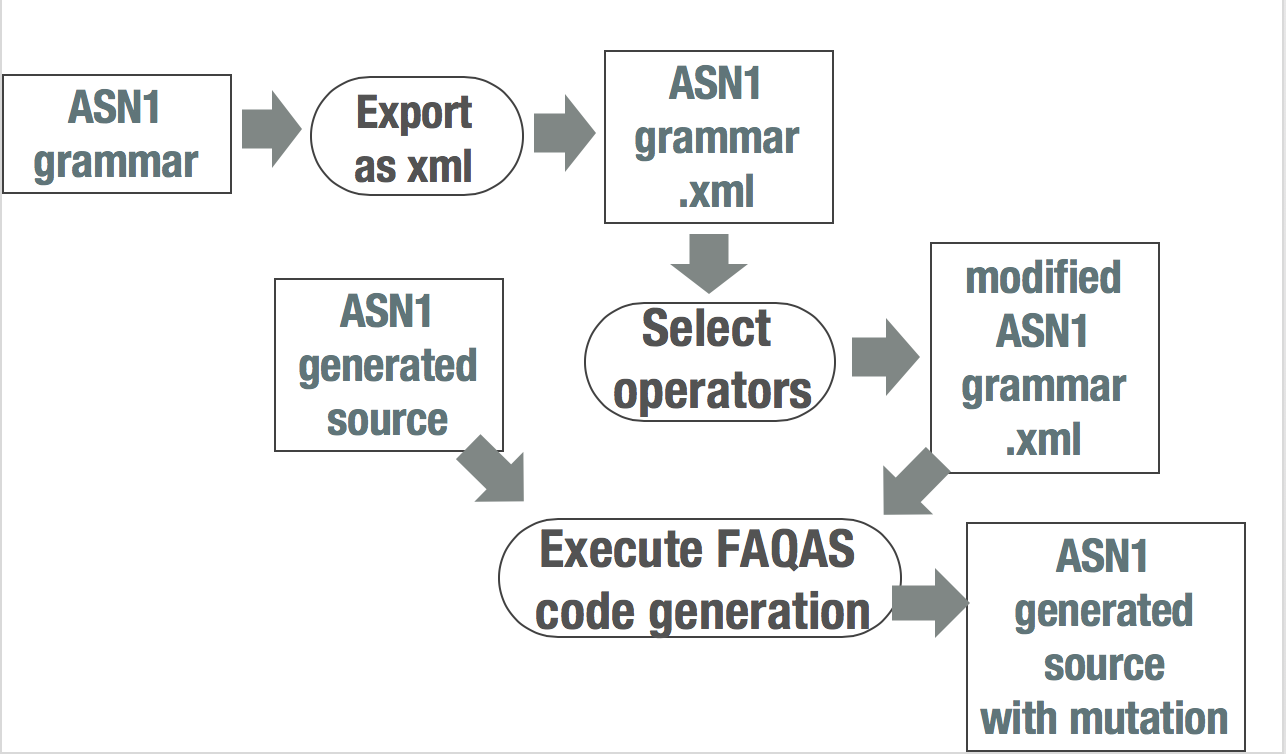
\includegraphics[width=12cm]{images/ASN1mutationProces}
      \caption{Data-driven probes generation process for ASN1.}
      \label{fig:ASN1ProbesGeneration}
\end{figure}








\clearpage
\subsection{FAQAS Data Mutation API and Probes}
\label{sec:FAQASDataMutationProbes}

In FAQAS, the data-driven mutation testing API is automatically generated from the fault model provided by engineers. Data mutation probes are either manually implemented by software engineers (in the case data mutation should target an ad-hoc communication layer that works with data buffers) or automatically generated by the toolset (in the case data mutation should target an ASN.1-based communication layer).

Section~\ref{sec:FAQASDataMutationProbesBuffer} describes the case of data buffers (i.e., C arrays).
Section~\ref{sec:FAQASDataMutationProbesASN} describes the case of ASN.1.


\subsubsection{Data Mutation for Data Buffers}
\label{sec:FAQASDataMutationProbesBuffer}

Figure~\ref{fig:DataDrivenBufferProcess} provides an overview of the envisioned data mutation process. 
The engineer prepares a single specification file for all the fault models that work with data buffers of a same time (e.g., int). The fault model specification is used by the FAQAS generator to automatically generate the mutation API. The engineer, then, modifies the source code of the SUT to add invocations to the mutation probes provided by the FAQAS API. 

Finally, the engineer iteratively executes the compiler in a loop to generate a different executable of the SUT for each mutation operation to perform.
The source code of the SUT is the same for all the fault models working on a data buffer of the same type. A configuration option (i.e., a \emph{define directive}) passed to the compiler is what drives the configuration of the specific mutation operation to be performed. 
More precisely, the engineer executes the compiled with the directive \EMPH{-DMUTATIONOPT=i}, where \emph{i} is a value between 0 and \emph{max}. The value \emph{max} coincides with the
overall number of mutation operation instances. An \INDEX{instance of a mutation operation} is a mutation operation that belongs to a mutation operator defined for a specific data item of the fault model. For the fault model in Table in \ref{table:faultModel:example} we have 6 instances, one for each data item except for data item 2, whose VOR fault class includes two mutation operations.

\begin{figure}[tb]
  \centering
    \includegraphics{images/DataDrivenBufferProcess}
      \caption{Data-driven mutation process for buffered data.}
      \label{fig:DataDrivenBufferProcess}
\end{figure}

The code that invokes the automatically generated probe is manually inserted by the engineer as shown in Listing~\ref{probesExample}.
The logic of the mutation probes is predefined and shared by all the mutation probes. What determines the different behaviours is the fault model.
The definition of the fault model is automatically generated in a \EMPH{C struct} (see Listing~\ref{faultModelExample}). 
The backbone data structures are predefined an provided in Listing~\ref{faultModelStructure}.

The code of the mutation probe is shown in Listing~\ref{mutationProbe}. It works by identifying the data item to mutate, the mutation operator to apply, and the mutation operation to execute by invoking methods \EMPH{\_FAQAS\_selectItem},
\EMPH{\_FAQAS\_selectOperator}, and \EMPH{\_FAQAS\_selectOperation}, respectively. The implementation of these three methods is automatically generated based on the fault model definition file.
An example is shown in Listing~\ref{selectors}. The runtime behaviour depends on the variable \EMPH{MUTATION}, whose value depends on the option passed at compile time. 
The variable \EMPH{MUTATION} uniquely identifies an instance of a mutation operation.
% (i.e., a mutation operation that belongs to a mutation operator defined for a specific data item of the fault model).

% !TEX root =  ../MAIN.tex

\begin{minipage}{15cm}
\begin{lstlisting}[style=CStyle, caption=Example of a data-driven mutation probes., label=probesExample, mathescape=true]


int receiveData()
{

    std::vector<char> v = connectAndReceiveData(); //function that receives data

    //MANUALLY ADDED PROBE
    FaultModel *fm = _FAQAS_IfHK_FM();
    _FAQAS_mutate(v->data(),fm);
    //MANUALLY ADDED PROBE END


}
\end{lstlisting}
\end{minipage}



% !TEX root =  ../MAIN.tex

\begin{minipage}{15cm}
\begin{lstlisting}[style=CStyle, caption=Example of generated fault models in C., label=faultModelExample, mathescape=true]
#define SIZE_IfHK 4
#define SIZE_IfStatus 1


struct FaultModel* _FAQAS_IfHK_FM(){
FaultModel *fm = _FAQAS_create_FM(SIZE_IfHK);

fm->items[0].operators[0].type=BF;
fm->items[0].operators[0].min=0;
fm->items[0].operators[0].max=0;
fm->items[0].operators[0].state=-1;
fm->items[0].operatorsN=1;
fm->items[0].span=1;
fm->items[0].type=BIN;

fm->items[1].operators[0].type=VOR;
fm->items[1].operators[0].min=0;
fm->items[1].operators[0].max=5;
fm->items[1].operators[0].delta=1;
fm->items[1].operatorsN=1;
fm->items[1].span=1;
fm->items[1].type=INT;

fm->items[2].operators[0].type=BF;
fm->items[2].operators[0].min=0;
fm->items[2].operators[0].max=0;
fm->items[2].operators[0].state=-1;
fm->items[2].operatorsN=1;
fm->items[2].span=2;
fm->items[2].type=BIN;

fm->items[4].operators[0].type=BF;
fm->items[4].operators[0].min=0;
fm->items[4].operators[0].max=0;
fm->items[4].operators[0].state=-1;
fm->items[4].operatorsN=1;
fm->items[4].span=1;
fm->items[4].type=BIN;
return fm;
}
struct FaultModel* _FAQAS_IfStatus_FM(){
FaultModel *fm = _FAQAS_create_FM(SIZE_IfStatus);

fm->items[0].operators[0].type=BF;
fm->items[0].operators[0].min=0;
fm->items[0].operators[0].max=0;
fm->items[0].operators[0].state=-1;
fm->items[0].operatorsN=1;
fm->items[0].span=1;
fm->items[0].type=BIN;
return fm;
}
\end{lstlisting}
\end{minipage}



% !TEX root =  ../MAIN.tex

\begin{minipage}{15cm}
\begin{lstlisting}[style=CStyle, caption=Fault model data structures., label=faultModelStructure, mathescape=true]
#define MAX_OPS 10
#define ITEMS 10


int MUTATION=MUTATIONOPT;

enum DataType {
    INT,
    FLOAT,
    DOUBLE,
    BIN
};

enum MutationType{
    BF,
    IV,
    VOR,
    VAT,
    VBT,
    INV
};

int _FAQAS_mutated = 0;

struct MutationOperator {
    MutationType type;
    int min;
    int max;
    int delta;
    int state;
};

struct DataItem {
    DataType type;
    int span;
    int operatorsN;
    struct MutationOperator operators[MAX_OPS];
};

struct FaultModel {
    int itemsN;
    struct DataItem *items;
};

\end{lstlisting}
\end{minipage}



% !TEX root =  ../MAIN.tex

\begin{minipage}{15cm}
\begin{lstlisting}[style=CStyle, caption=Automatically generated selectors., label=selectors, mathescape=true]
int _FAQAS_selectItem(FaultModel *dm){
if ( MUTATION == 0 )
    return 0;
if ( MUTATION == 1 )
    return 1;
if ( MUTATION == 2 )
    return 1;
if ( MUTATION == 3 )
    return 2;
if ( MUTATION == 4 )
    return 4;
if ( MUTATION == 5 )
    return 0;
}
int _FAQAS_selectOperator(FaultModel *dm){
if ( MUTATION == 0 )
    return 0;
if ( MUTATION == 1 )
    return 0;
if ( MUTATION == 2 )
    return 0;
if ( MUTATION == 3 )
    return 0;
if ( MUTATION == 4 )
    return 0;
if ( MUTATION == 5 )
    return 0;
}
int _FAQAS_selectOperation(FaultModel *dm){
if ( MUTATION == 0 )
    return 0;
if ( MUTATION == 1 )
    return 0;
if ( MUTATION == 2 )
    return 1;
if ( MUTATION == 3 )
    return 0;
if ( MUTATION == 4 )
    return 0;
if ( MUTATION == 5 )
    return 0;
}
\end{lstlisting}
\end{minipage}



% !TEX root =  ../MAIN.tex

\begin{minipage}{15cm}
\begin{lstlisting}[style=CStyle, caption=Mutation API function., label=mutationProbe, mathescape=true]
int _FAQAS_mutate( int *data, FaultModel *fm ){
    if ( _FAQAS_mutated == 1 )
    return 0;

    if ( MUTATION == -1 )
    return 0;

    int pos = _FAQAS_selectItem(fm);
    int op = _FAQAS_selectOperator(fm);
    int opt = _FAQAS_selectOperation(fm);

    int valueInt;
    int valueBin;
    double valueDouble;


    //Load the data in the appripriate var
    if ( fm->items[pos].type == BIN ){
        valueBin = (int) data[pos];
    }
    if ( fm->items[pos].type == INT ){
        valueInt = (int) data[pos];
    }
    if ( fm->items[pos].type == DOUBLE ){
        valueDouble = (double) data[pos];
    }
...
    MutationOperator *OP = &(fm->items[pos].operators[op]);    
...     
        if ( OP->type == VOR ){
        if ( fm->items[pos].type == INT ){

            if ( opt == 0 ){
                valueInt = OP->min-OP->delta;
            } else if (opt == 1 ){
                valueInt = OP->max+OP->delta;
            } else {
                //ERROR
            }
            _FAQAS_mutated = 1;
        }

...

    }

...

    if ( _FAQAS_mutated != 1 ){
        return 0;
    }

    //
    //Store the data
    //
    //FIXME: handle span
    if ( fm->items[pos].type == INT ){
        data[pos] = valueInt;
    }
    if ( fm->items[pos].type == DOUBLE ){
        data[pos] = valueDouble;
    }
    if ( fm->items[pos].type == BIN ){
        data[pos] = valueBin;
    }
    
    ...

    
\end{lstlisting}
\end{minipage}




\subsubsection{Data Mutation Probes for ASN.1}
\label{sec:FAQASDataMutationProbesASN}

\TODO{This section still needs to be written. We may put a sequence diagram that show that at the beginning the probe loads the info about the mutation operation instance to execute and execute it if feasible.}

\clearpage
\subsection{Test suite execution}
\label{sec:mutantsExecution}

During data mutation the test suite is executed a number of times that depends on a stopping criterion chosen by the engineer. We foresee two possible stopping criteria (1) every test case is run with every data mutation operation (hereafter, test coverage stopping criterion)
%, (2) exercise each data fault class (hereafter, fault coverage stopping criterion)
, and (2) a sample of the available data mutation operations has been executed with every test case (hereafter, sampling stopping criterion).

% !TEX root =  ../Main.tex

%\newcommand{\INDA}{10}
%\newcommand{\INDB}{15}
%\newcommand{\INDC}{5}

%\vspace{-3mm}
\begin{figure}[tb]

\begin{algorithmic}[1]

%\footnotesize
\scriptsize
\Require \emph{EMOS}, set of SUT executables, each one implementing one mutation operation (EMO)
\Require \emph{TS}, the test suite of the SUT
% (source inputs, follow-up inputs, output data).


\State \hspace{5 mm} \textbf{for each} $t$ in $TS$ \label{alg:prioritize:prel}
\State \hspace{10 mm} \textbf{execute} $t$ to track the data items exercised by t

\State \textbf{for each} $EMO$ in $EMO$ \label{alg:dataProcess:repeat}
\State \hspace{5 mm} \textbf{for each} $t$ in $TS$ \label{alg:prioritize:t}
\State \hspace{10 mm} \textbf{if} $t$ contains a data item that can be mutated with $EMO$ \label{alg:prioritize:cove}
\State \hspace{15 mm} \textbf{execute} $t$ with $EMO$
\State \hspace{15 mm} \textbf{if} $t$ fails or invalid data detected
\State \hspace{\INDB mm} \textbf{break} \label{alg:prioritize:stop}



\end{algorithmic}
\vspace{-3mm}
\caption{Algorithm for executing data-driven mutation testing with test coverage stopping criterion}
%\vspace{-0.2cm}
\label{alg:dataProcess}
\end{figure}




Figure~\ref{alg:dataProcess} shows how the data mutation process should be iterated with
 the \EMPH{test coverage stopping criterion}. 

A preliminary execution of the test suite against a mutated executable configured to simply track the data items exchanged during each test case execution (Line~\ref{alg:prioritize:prel}), enable us to determine which test cases exercise the data items targeted by a specific mutation operation instance.

 For each mutation operation instance (Line~\ref{alg:dataProcess:repeat}), we execute every test case of the test suite (Line~\ref{alg:prioritize:t}), if it exercise the data item targeted by the mutation operation (Line~\ref{alg:prioritize:cove}), till one of the test cases kills the mutant, i.e., it fails or detects the presence of invalid data and trigger a fault tolerant mechanism (Line~\ref{alg:prioritize:stop}).
 We can configure the data mutation API to inject a single data fault or to mutate all the data where the mutation operation instance can be applied (this is useful to simulate a bit that is always flipped because of hardware fault).
The mutation algorithm can either mutate the first mutable data item observed or randomly decide whether to mutate the mutable data item. The second case enables the mutation of data items exchanged after long components interactions. However, it requires the repeated execution of a test case in case the mutation has not been performed but a data item could have been mutated. 



%With the fault coverage stopping criterion the full test suite is executed multiple times till all the possible data fault classes had been injected at least once (for the full test suite).
%A data fault class is no longer injected after it has already been injected in a test case of the test suite.
%The mutation algorithm can either mutate the first mutable data item observed or randomly decide whether to mutate the mutable data item.
%The repeated execution of a test case is terminated after it has been executed once without identifying any mutable data item.

With the \EMPH{sampling stopping criterion} we perform the same activities performed for the test coverage criterion except that the set of mutation operation instances to be performed is randomly sampled (e.g., only 5\% of the mutation operations are considered).



\clearpage
\section{Test Suite Augmentation} % (fold)
\label{sec:data:test_suite_augmentation}

\TODO{This section still needs to be written.}

%The test suite augmentation process concerns the definition of additional test cases to increase the mutation score.
%It consists of four activities \emph{Identify Test Inputs}, \emph{Generate Test Oracles}, \emph{Execute the SUT}, \emph{Fix the SUT}. 
%Despite these activities match the ones performed in the case of code-driven mutation testing, they are triggered and implemented in a different manner, as described below.
%
%
%
%In the presence of mutants not killed by test cases (i.e., when the \emph{\% of Mutants Killed} is not equal to 100\%), engineers are expected to improve the oracles of existing test cases. Indeed, the presence of mutants not killed by test cases indicates that the oracles of the test suite are not capable of detecting that the software is failing. 
%Automated approaches for performing this activity in the presence of system or integration test suites are not available and thus it needs to be performed manually.
%
%In the presence of operators not being applied (i.e., the \emph{\% Operators Applied} is not equal to 100\%), engineers are expected to generate new test inputs for the SUT that enable the application of all the mutation operators. 
%For example, in the case of the example in Figure~\ref{fig:DataDrivenSimpleExample}, engineers would need to implement test cases that trigger the exchange of \emph{DataMessages}.
%Fully automated approaches to generate test cases for data-driven mutation testing are unavailable; however, techniques that generate input data from scratch~\cite{gligoric2010test} or augment input data~\cite{DiNardo:TOSEM:2017} can be adopted. 
%Also, when the data used by test cases is generated by simulators, meta-heuristic search can be used to drive the generation of input data~\cite{Abdessalem:ICSE:2018}. 
%
%The execution of the SUT and the repair of the SUT are performed manually as in the case of code-driven data mutation.
%
%
%\TODO{Clarify if we generate test cases or not}
%
%Section~\ref{sec:testGenerationData} provides details about the existing solutions to  \emph{Identify Test Inputs} and \emph{Generate Test Oracles}.




%% !TEX root =  ../Main.tex

\begin{table}[tb]
\caption{Descriptions of software components.}
\label{table:caseStudies} 
\scriptsize
\centering
\begin{tabular}{|
@{\hspace{1pt}}p{12mm}
@{\hspace{2pt}}|
@{\hspace{1pt}}>{\raggedleft\arraybackslash}p{8mm}@{\hspace{1pt}}|
@{\hspace{1pt}}>{\raggedleft\arraybackslash}p{18mm}@{\hspace{1pt}}|
@{\hspace{1pt}}>{\raggedleft\arraybackslash}p{20mm}@{\hspace{1pt}}|
@{\hspace{1pt}}>{\raggedleft\arraybackslash}p{24mm}@{\hspace{1pt}}|
p{20mm}|}
\hline
\textbf{Component}&\textbf{LOC}&\textbf{Test suite type}&\textbf{\# Test cases}&\textbf{Statements} \textbf{coverage}\\
\hline
ESAIL& 74155 & System& 384 & 90.38\% \\
ESAIL$_S$& 2235 & System& 384 & 95.36\%\\
LIBGSCSP& 9836 & Integration& 89 & 63.10\%\\
LIBPARAM& 3179 & Integration& 170 & 77.60\%\\
LIBUTIL& 10576 & Unit& 201 & 83.20\%\\
MLFS& 5402 & Unit& 4042 & 100.00\%\\
%MLFS$_V$& 5402 & 4042 & 100.00\%\\
\hline
\end{tabular}

\end{table}

%% !TEX root = MAIN.tex

\chapter{Applicability to Space Software Standards}

To discuss the type of mutation testing (i.e., code-driven or data-driven) to consider within the different ECSS activities, we focus on the interactions exercised by different test levels (i.e., unit, integration, system, acceptance).  Figure~\ref{fig:mutationTestingVSTestingLevels} provides a generic overview of the interactions typically stressed by different test levels. Unit test cases focus on interactions within single units (e.g., functions belonging to a same source files) or few units belonging to a same component. Integration test cases trigger interactions between distinct units or multiple components. System test cases exercise interactions between all the components of the system. According to ECSS standards, system test cases might be executed on a host system with emulated hardware. Acceptance test cases exercise all the system components but in the operational environment (ECSS-E-ST-40C 4.2.6). For this reason, mutation testing cannot be adopted in the context of acceptance testing because the deployment of multiple version of the system (one for each mutant) might be particularly expensive and may lead to safety hazards.
 
 
\begin{figure}[h]
  \centering
    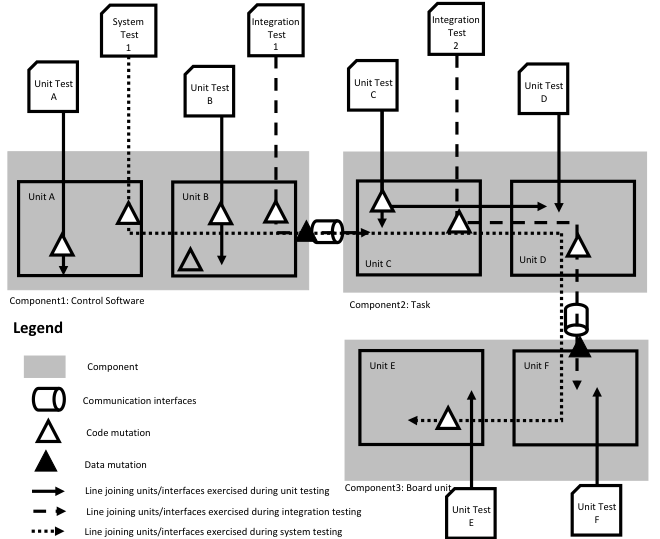
\includegraphics[width=10cm]{images/TestingLevels}
      \caption{Mutation Testing Approaches for Different Testing Levels.}
      \label{fig:mutationTestingVSTestingLevels}
\end{figure} 

%Test suite evaluation through code-driven mutation testing appear to be feasible for all the testing levels (i.e., unit, integration, and system), except acceptance testing for the reasons mentioned above. 

\INDEX{Unit testing} is the typical scenario in which code-driven mutation testing is adopted in other contexts, for this reason it should be targeted also in the case of space software.
In addition, code-driven test generation approaches based on static program analysis can be adopted to automatically generate unit test cases.
Data-driven mutation techniques, instead, are unlikely to be useful in the context of unit testing.
Indeed, Unit test cases do not verify the interaction between units but rely on stubs when the testing of  a unit requires the interaction with another component.
Also, although certain units focus on the communication with hardware components (e.g., chips) applying data-driven mutation techniques in that context would simply lead to a form of robustness testing targeting hardware components.


In the context of \INDEX{integration testing}, the use of traditional code-driven mutation operators conceived for unit testing may lead to an inadequate assessment of the test suite quality.
Indeed, an integration test suite is not expected to detect functional problems of single units; for this reason, the mutation score for an integration test suite computed with mutation operators for functional faults (e.g., the sufficient set) may not adequately measure the quality of the test suite.
The adoption of operators dedicated to integration testing might be evaluated instead~\cite{grechanik2016mutation,delamaro2001proteum}; however, these approaches target API methods but they do not inject higher level errors (e.g., errors in the structure of the data generated by multiple components). For this reason, in FAQAS, we suggest to rely on data-driven mutation testing to assess the quality of integration test suites. Test case generation approaches based on static analysis may be used, in principle, to support the generation of test cases that kill data-driven mutants; however, to date, the manual implementation of missing test cases remains the most appropriate solution  (see Section~\ref{sec:data:test_suite_augmentation}).


In the context of \INDEX{system testing}, both code-driven and data-driven mutation can be applied. However, the long execution time required by system test cases may emphasize the scalability problems of mutation testing; the evaluation of solutions for such scalability problems are part of the FAQAS objectives.
%However, within FAQAS, we expect to develop solutions that will enable mutation testing to scale with large system test suites. 
Depending on the development process, system-level test cases may focus only on specific features of the system under test, for this reason system-level test cases may not reach 100\% statement coverage. For the same reason, system-level test cases may lead to a mutation score that is lower than the one achieved with unit test cases. We suggest to compute the mutation score by considering all the available test suites (i.e., a mutant is killed if at least one test case of any available test suite fails). Although software testing literature report results that show the feasibility of relying on model-based test generation to automatically generate system level test suites (see Deliverable D1), such approaches are preliminary and will not be evaluated in the context of FAQAS. In the context of FAQAS, we do not aim to automatically generate system-level test cases.

\begin{figure}[h]
  \centering
    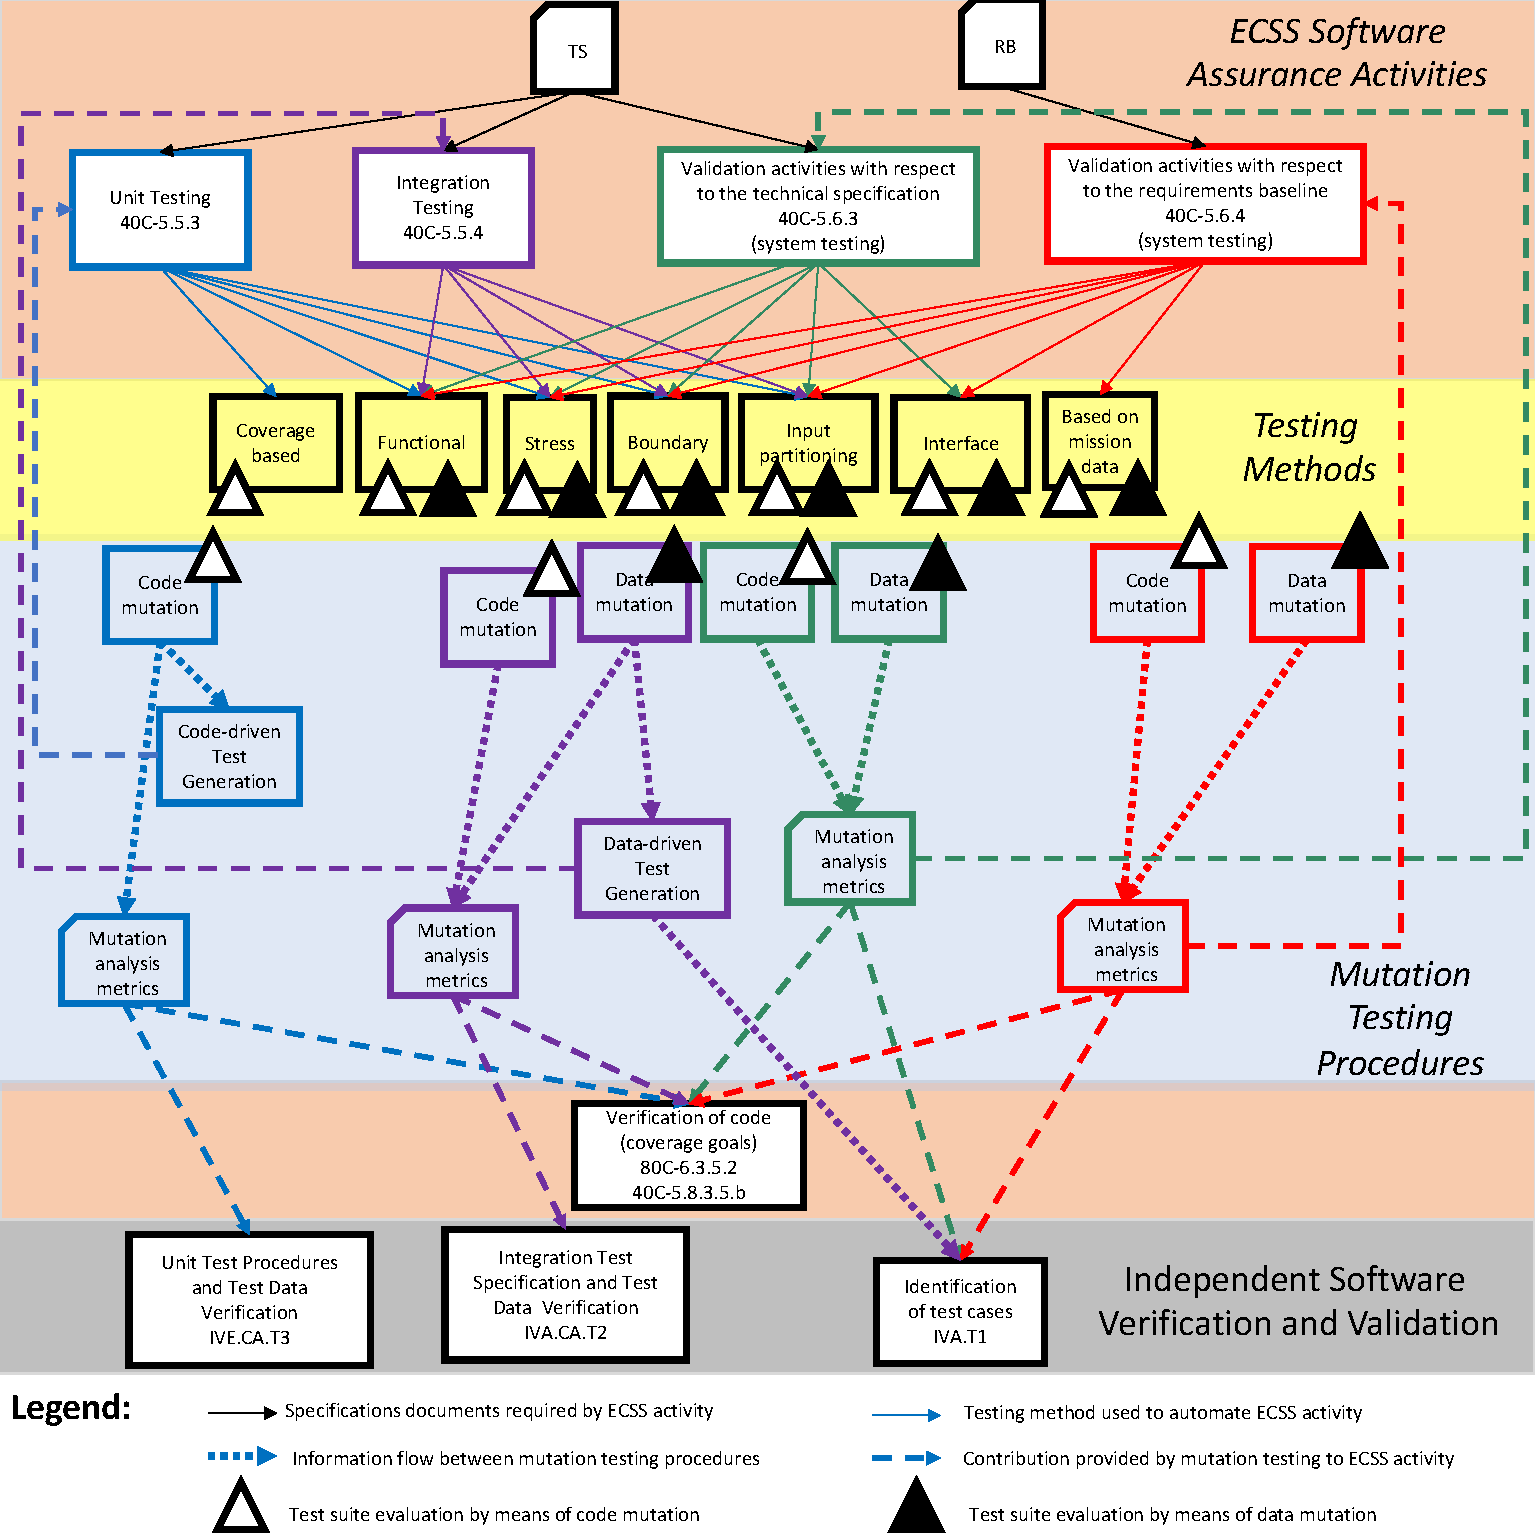
\includegraphics[width=0.9\textwidth]{images/ECSSTesting}
      \caption{Relations between ECSS activities and activities of the mutation testing process.}
      \label{fig:ECSSTesting}
\end{figure} 

Figure~\ref{fig:ECSSTesting} shows the envisioned relationships between ECSS software testing practices and the main activities of the mutation testing process (i.e., code mutation, data mutation, code-based generation, model-based generation, and generation of the mutation score). These relationships guide the definition of a mutation testing process integrated with ECSS standards. 
 
In Figure~\ref{fig:ECSSTesting}, black arrows show the specifications documents (i.e., Technical Specifications and Requirement Baselines) used to support ECSS testing activities (i.e., Unit Testing, Integration Testing, Validation activities with respect to the technical specification and Validation activities with respect to the requirements baselines). Colored arrows are used to associate ECSS activities to specific testing methods suggested in the ECSS standard (e.g., mission data is used for ECSS-E-ST-40C-5.6.4). Triangles are used to indicate which type of mutation testing (i.e., code-driven or data-driven) is likely applicable when a specific testing method is applied. White triangles are used to indicate that code mutation can be applied with a certain testing method, black triangles are used for data mutation. 

Concerning the type of mutation activity associated to each testing method, we observe that although code-driven mutation might be used for all the testing methods in use, it is unlikely to be adopted when mission data is used for testing because mission data might lead to long software executions that cannot be repeated for all the mutants. Data-driven mutation, instead, is unlikely to be used with coverage based testing which often targets unit tests. 

Test case generation based on static analysis can be used in the context of unit and integration testing for both code-driven and data-driven mutation testing. In the system testing context, model-based generation might be adopted; however, it is not covered by FAQAS.

In Figure~\ref{fig:ECSSTesting}, dashed arrows show how the mutation testing procedures can contribute to ECSS activities. The mutation score computed by the mutation testing process might be used to support verification activities; more precisely, it might be used as an additional coverage metric for the activities described in ECSS-Q-ST-80C 6.3.5.2 and ECSS-E-ST-40C 5.8.3.5.b. Independent Software Verification and Validation~\cite{ESAISVV} can benefit from the mutation testing process as well. The mutation score can support Unit Test Procedures and Test Data Verification (IVE.CA.T3 in~\cite{ESAISVV}) and Integration Test Specification and Test Data Verification (IVA.CA.T2 in~\cite{ESAISVV}). Finally, model-based test generation and mutation score will support ISVV during the identification of test cases (IVA.T1 in~\cite{ESAISVV}).



\newpage

\appendix


%\chapter{ESAIL Fault Model}
%\label{appendix:esailFM}
%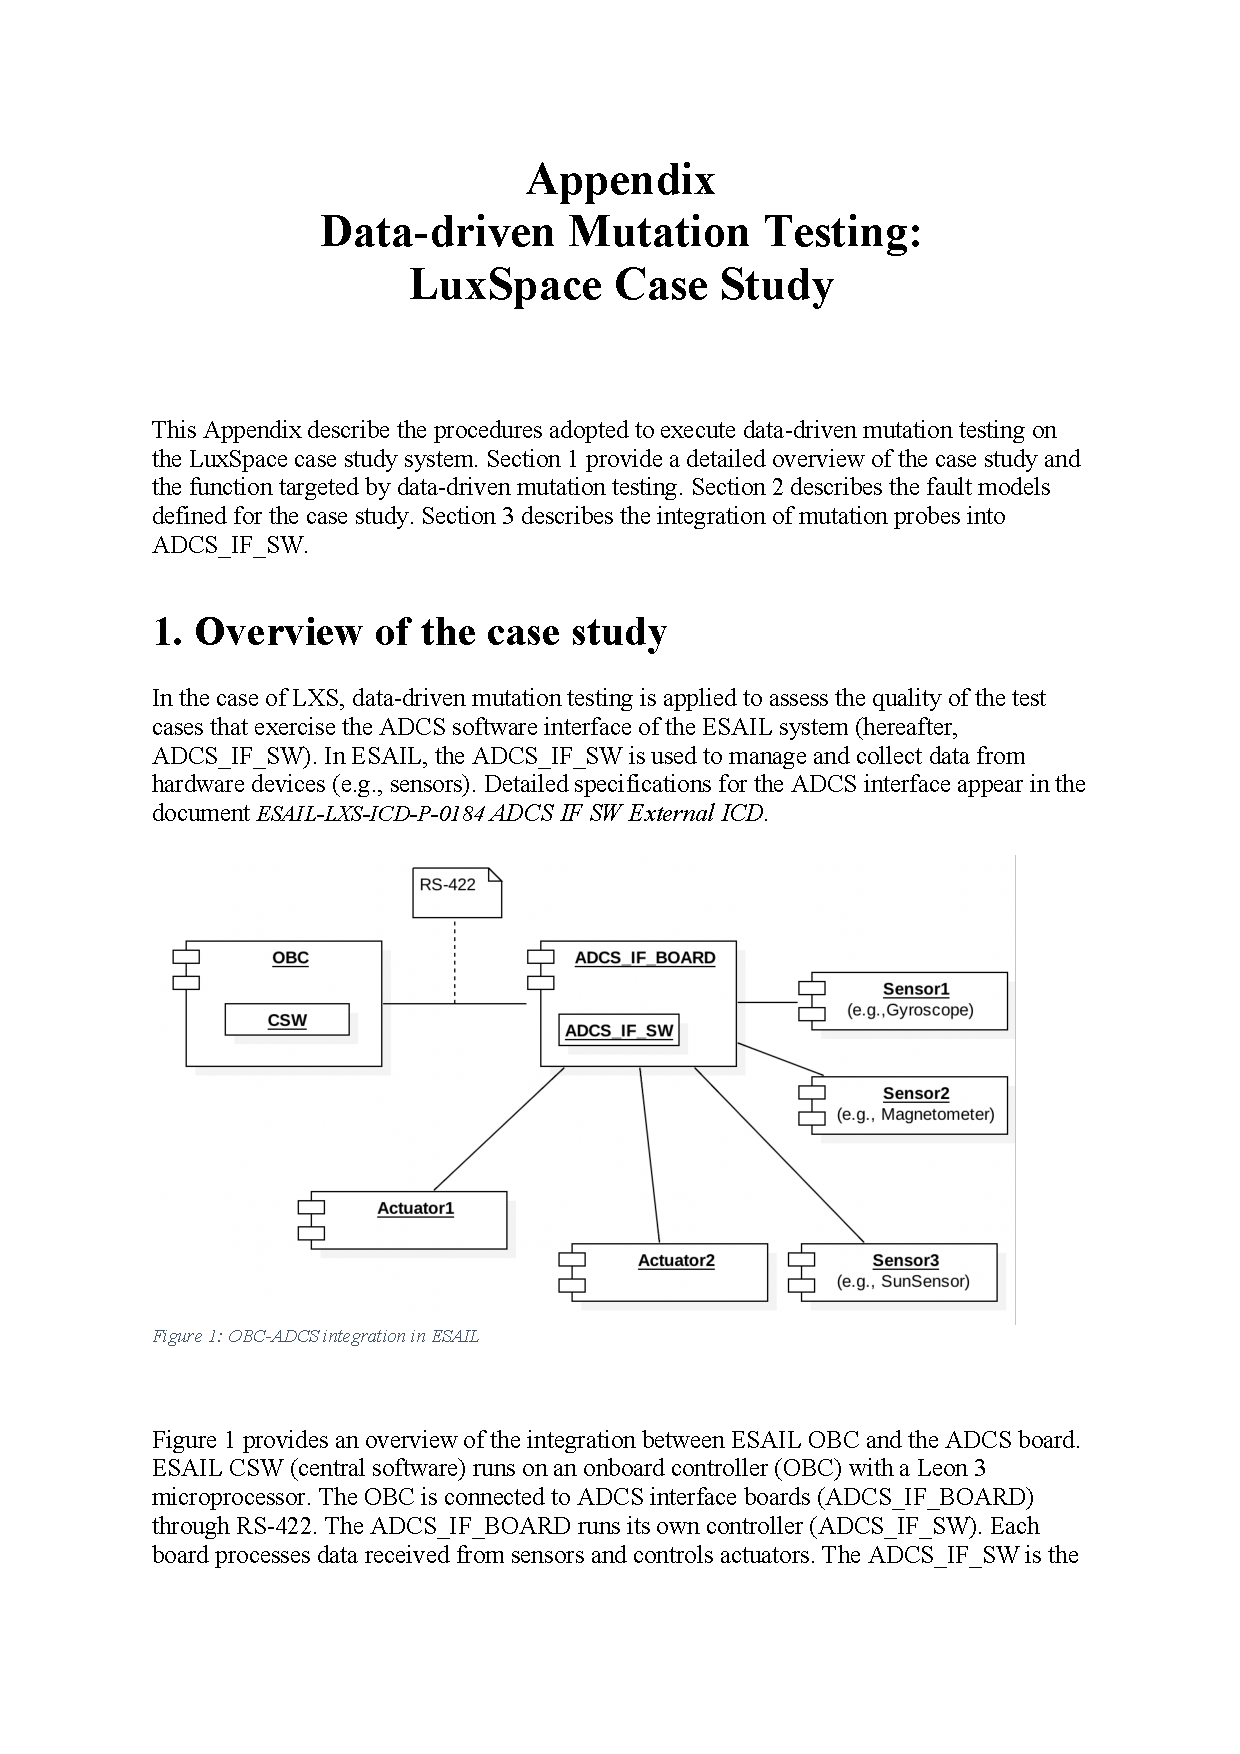
\includepdf[pages=-,scale=0.9,offset=0mm -75]{faultModels/ESAIL_ADCS.pdf}
%
%\textbf{End of Appendix~\ref{appendix:esailFM}}

   
%\clearpage
%% !TEX root = MAIN.tex
\chapter{ESA Revisions}

%% !TEX root = MAIN.tex

\section{Responses to ESA comments provided on 12.04.2021}
\label{sec:ESA:comments:1}

Comments IDs appear also in the main document next to the text modified to address the comment. To save space in the main text, the prefix \emph{ITSR-SSS-PABG-} has been abbreviated as \emph{P-}.

\setlength\LTleft{0pt}
\setlength\LTright{0pt}
\tiny 
%@{\extracolsep{\fill}}
\begin{longtable}{|p{1.5cm}|p{12cm}|@{}}
%\caption{\normalsize .}
%\label{table:comments:responses} 
\textbf{Comment ID}&\textbf{Response}\\
\\
\hline
P-1&
\begin{minipage}{12cm}
We will need to discuss the detail of the merge of the two specifications during the review meeting.
\end{minipage}\\
\\
\hline

P-2&
\begin{minipage}{12cm}
Done.
\end{minipage}\\
\\
\hline

P-3&
\begin{minipage}{12cm}
Done.
\end{minipage}\\
\\
\hline

P-4&
\begin{minipage}{12cm}
Done.
\end{minipage}\\
\\
\hline

P-5&
\begin{minipage}{12cm}
Done.
\end{minipage}\\
\\
\hline

P-6&
\begin{minipage}{12cm}
Done.
\end{minipage}\\
\\
\hline

P-7&
\begin{minipage}{12cm}
Done.
\end{minipage}\\
\\
\hline

P-8&
\begin{minipage}{12cm}
Done.
\end{minipage}\\
\\
\hline

P-9&
\begin{minipage}{12cm}
It is worth discussing if it makes sense to perform mutation analysis without code coverage.
\end{minipage}\\
\\
\hline


P-10&
\begin{minipage}{12cm}
We always generate all the mutants because it's fast. End-users have the option to execute a subset of them.
\end{minipage}\\
\\
\hline

P-11&
\begin{minipage}{12cm}
We changed a sentence, but this requirement is long because we had to provide an explanation missing from D2.
\end{minipage}\\
\\
\hline

P-12&
\begin{minipage}{12cm}
\end{minipage}\\
\\
\hline

P-13&
\begin{minipage}{12cm}
\end{minipage}\\
See P-8\\
\hline

P-14&
\begin{minipage}{12cm}
\end{minipage}\\
Action item. To be done for the end of WP3.\\
\hline


P-15&
\begin{minipage}{12cm}
TOD
\end{minipage}\\
\hline

P-16&
\begin{minipage}{12cm}
Done.
\end{minipage}\\
\hline

P-17&
\begin{minipage}{12cm}
We will provide a table for end of WP3.
\end{minipage}\\
\hline
                                                
\end{longtable}
\normalsize

\clearpage

% !TEX root = MutationTestingSurvey.tex

\section{Responses to ESA comments provided on 03.04.2020}
\label{sec:ESA:comments:2}


\setlength\LTleft{0pt}
\setlength\LTright{0pt}
\tiny 
\begin{longtable}{|p{1.5cm}|p{12cm}|@{}}
\label{table:comments:responses} 
\textbf{Comment ID}&\textbf{Comment and Response (below)}\\
\\
\midrule
C6 \& C7
&
Have you seen numbers for this mutation score and threshold in the literature? Is this something to be checked during the use case evaluation?
\\
\cmidrule{2-2}
&
We have addressed the comments above.
\TODO{OScar: please check if the survey of Papadakis say something aboth teh threshold (C7)}
\\
\hline
C8
&
Elaborate a bit more on C8 (pros and cons of doing mutation at source code / IR/ Assembly/ Executable);
\\
\cmidrule{2-2}
&
\TODO{Oscar: you may refer to taht paper of Darko Marinov and Co. to say IR is not good}
\\
\hline
C31
&
What is this sufficient set of operators?
\\
\cmidrule{2-2}
&
\TODO{Oscar}
\\
\hline
C32
&
Can you please add the solution for this example? i.e. do we need two different test cases of isPalindrome to detect both mutants?
\\
\cmidrule{2-2}
&
\TODO{Oscar}
\\
\hline
C33
&
Even if the objectives are complementary, both of them should be pursued for a data mutation testing approach?
\\
\cmidrule{2-2}
&
We have addressed the comment above.
\\
\hline
C34
&
The sentence sounds weird... To automate?? Is this activity something that can be automated?
\\
\cmidrule{2-2}
&
We have addressed the comment above by clarifying our text.
\\
\hline
C35
&
Is it possible to add an example of equivalent and redundant mutants?
\\
\cmidrule{2-2}
&
We have added the requested examples.
\\
\hline
C36
&
\begin{minipage}{12cm}
Related to automation, in my opinion, what it is key is that the test assessment process (for both data and code mutation) is as much automated as possible.\\

Automated generation of test cases is a very nice to have. In an industrial environment, let's say that we could afford spending some time to manually augment the test suite.\\

You may consider this to prioritize tasks within this activity.
\end{minipage}
\\
\cmidrule{2-2}
&
We agree on the comment. No need to change the text in this deliverable.
\\
\hline
C37
&
Are we missing a chapter to address the Generation of Test Oracles?\\
\cmidrule{2-2}
&
We have added a section concerning generation of test oracles for code-driven mutation testing (Section~\ref{sec:oraclesGeneration:codeDriven}) and data-driven mutation testing 
(Section~\ref{sec:oracles:dataMutation}).
\\
\hline
C38
&
\begin{minipage}{12cm}
a. From these Case Studies, is there any that you would like to try out within FAQAS?\\

b. One thing that we may need for FAQAS framework is to have kind of a test suite allowing to test the tool, and also to test the tool when new versions will be produced. Would any of these case studies fulfill that?
\end{minipage}
\\
\cmidrule{2-2}
&
We have discussed this topics by voice.
\\
\hline
C39
&
Do you have any information on the kind of test suite? (e.g. is it unit testing, system testing, ...)
\\
\cmidrule{2-2}
&
\TODO{}
\\
\hline
C40
&
Are these case studies focused on Code-Mutation, Data-Mutation, or both?\\
\cmidrule{2-2}
&
\TODO{}
\\
\hline
C41
&
Is there any meaningful conclusion (positive or negative) from those industrial case studies?\\
\cmidrule{2-2}
&
\TODO{}
\\
\hline
C42
&
\begin{minipage}{12cm}
Can we make a conclusion paragraph on this?\\

e.g. No tool based on mutation testing is known to be used within an industrial software development environment\\
e.g. Mutation testing is seen applied mainly within research environments\\
etc, etc
\end{minipage}
\\
\cmidrule{2-2}
&
\TODO{}
\\
\hline
C43
&
Is there any of these trends that could be meaningful to explore?
\\
\cmidrule{2-2}
&
\TODO{}
\\
\hline
C44
&
\begin{minipage}{12cm}
	\begin{itemize}
		\item Is there any particular trend for Code-Based mutation testing? (e.g. research is on-going or vanishing, the way to apply it, the type of operators used, the tools supporting it, ...)
		\item Any particular trend for Data-Based mutation testing?
	\end{itemize}
\end{minipage}
\\
\cmidrule{2-2}
&
\TODO{}
\\
\hline
C45&
\begin{minipage}{12cm}
D1 is fulfilling well requirement R1-1 as in the SoW. There is only one exception, on the red sentence below:\\

[R1-1.c] The applications of mutation testing (e.g. code and data mutation, test-suite evaluation, test cases generation, test-data generation, \textcolor{red}{code quality improvement}, ...)\\

The evaluation of code quality improvement is to be looked at. Indeed, this would be a secondary objective of applying mutation testing on space systems, but we would like to understand if mutation testing could help improve the code quality or not.\\
\end{minipage}
\\
\cmidrule{2-2}
&
\begin{minipage}{12cm}
We added a paragraph on Chapter~\ref{chapter:trends} explaining that there are no works in literature about quality code improvement based on code-driven mutation testing.
\end{minipage}
\\

\bottomrule                                                             
\end{longtable}
\normalsize

\clearpage


%\clearpage

\printindex

\bibliographystyle{IEEEtran}
\bibliography{bibliography}


\end{document}  